\chapter{Results and Discussion}
This chapter presents the results gathered during the development and testing phases of ClassiFish: A Mobile Application for Fish Classification and Species Information Using YOLO-v11 with User Feedback Reporting. It discusses the outcomes of the model's training, validation, and testing, as well as the system’s ability to correctly classify fish species. 

%\textbf{\footnote{For more information see: \url{http://rc.rcjournal.com/content/49/10/1229.short}}}

\section{Data Collection}                                          
A total of 150 raw images were obtained for each of the 18 fish species, resulting in a total of 2,700 raw fish images for the dataset. Figures~\ref{fig: Bangus and Maya-maya} to ~\ref{fig: Anduhaw and Sulid} below show sample images of each of the 18 different fish species.

\begin{figure}[H]
    \centering
    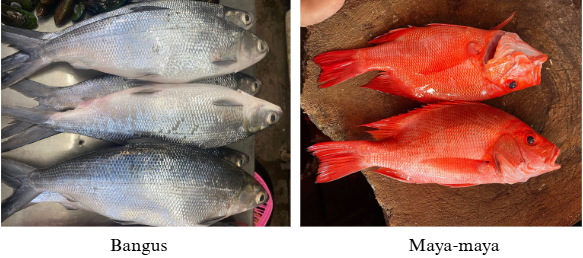
\includegraphics[width=0.85\textwidth]{images/images/bangus_maya.png}
    \caption{Sample Image of Bangus and Maya-maya} 
    \label{fig: Bangus and Maya-maya}
\end{figure}

\begin{figure}[H]
    \centering
    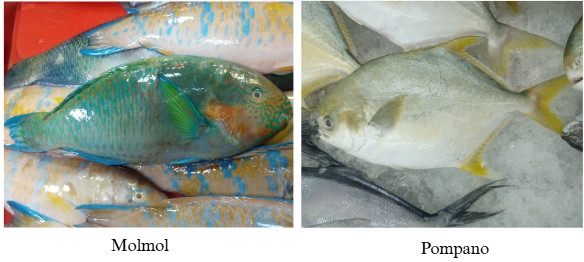
\includegraphics[width=0.85\textwidth]{images/images/molmol_pompano.png}
    \caption{Sample Image of Molmol and Pompano} 
    \label{fig: Molmol and Pompano}
\end{figure}

\begin{figure}[H]
    \centering
    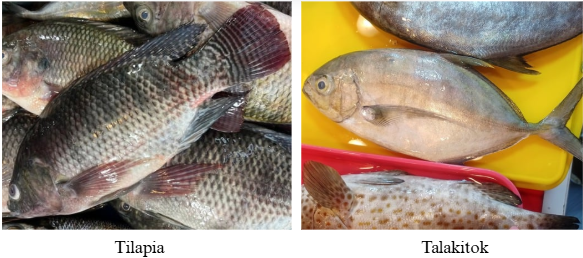
\includegraphics[width=0.85\textwidth]{images/images/tilapia_talakitok.png}
    \caption{Sample Image of Tilapia and Talakitok} 
    \label{fig: Tilapia and Talakitok}
\end{figure}

\begin{figure}[H]
    \centering
    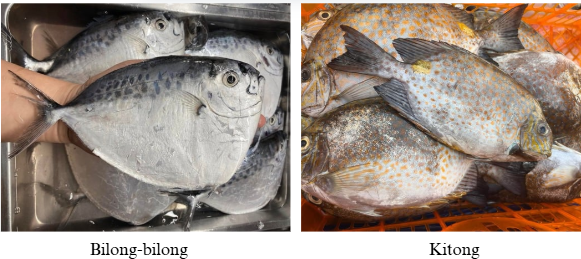
\includegraphics[width=0.8\textwidth]{images/images/bilong_kitong.png}
    \caption{Sample Image of Bilong-bilong and Kitong} 
    \label{fig: Bilong-bilong and Talakitok}
\end{figure}

\begin{figure}[H]
    \centering
    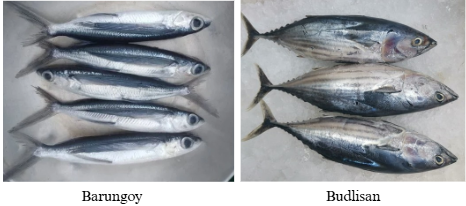
\includegraphics[width=0.9\textwidth]{images/images/barungoy_budlisan.png}
    \caption{Sample Image of Barungoy and Budlisan} 
    \label{fig: Barungoy and Budlisan}
\end{figure}

\begin{figure}[H]
    \centering
    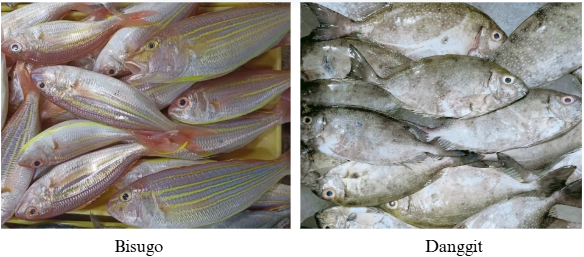
\includegraphics[width=0.9\textwidth]{images/images/bisugo_danggit.png}
    \caption{Sample Image of Bisugo and Danggit} 
    \label{fig: Bisugo and Danggit}
\end{figure}

\begin{figure}[H]
    \centering
    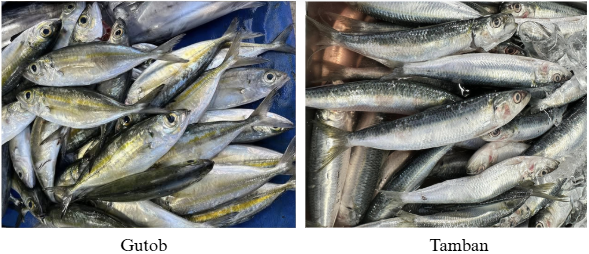
\includegraphics[width=0.9\textwidth]{images/images/gutob_tamban.png}
    \caption{Sample Image of Gutob and Tamban} 
    \label{fig: Gutob and Tamban}
\end{figure}

\begin{figure}[H]
    \centering
    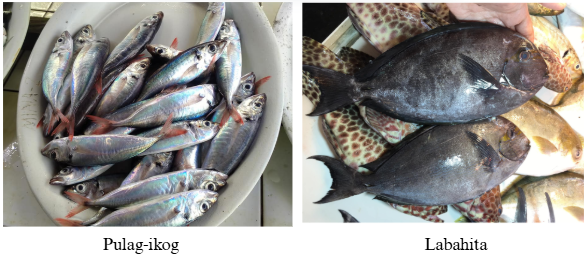
\includegraphics[width=0.9\textwidth]{images/images/pulag_ikog_labahita.png}
    \caption{Sample Image of Pulag-ikog and Labahita} 
    \label{fig: Pulag-ikog and Labahita}
\end{figure} 

\begin{figure}[H]
    \centering
    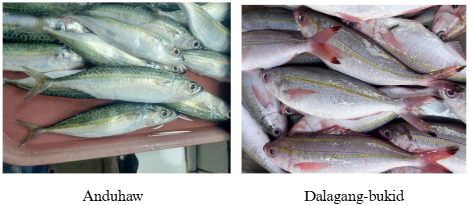
\includegraphics[width=0.9\textwidth]{images/images/anduhaw_dalagangbukid.png}
    \caption{Sample Image of Anduhaw and Sulid} 
    \label{fig: Anduhaw and Sulid}
\end{figure} 

\section{Data Preprocessing}
In this section, the data preprocessing involves cleaning, transforming , and organizing raw data to prepare it for training the model.

\subsection{Image Annotation}
The captured images of fish species were stored in Google Drive and then imported to Label Studio for annotation. The image annotation was done manually by drawing bounding boxes around the full body of the fish, with each box assigned coordinates and class labels corresponding to the respective species. Figure~\ref{fig:fish_annotation} below shows an example of the Fish Image Annotation in Label Studio.

\begin{figure}[H]
    \centering
    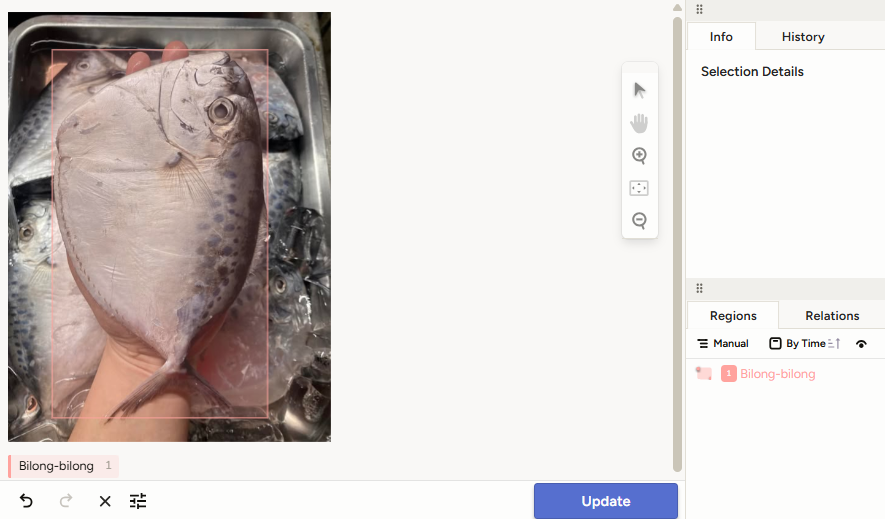
\includegraphics[width=0.99\textwidth,height=0.6\textheight,keepaspectratio]{images/images/fish_annotation.png}
    \caption{Fish Image Annotation} 
    \label{fig:fish_annotation}
\end{figure}

\subsection{Dataset Consolidation and Classes Remapping}

During the annotation phase, each of the 18 fish species was annotated separately in Label Studio, resulting in 18 distinct project folders, one for each species. To prepare the dataset for YOLOv11 training, it requires all images and corresponding label files to reside in a single directory, these 18 fish species-specific folders were consolidated into one unified folder. 

This consolidation ensured that the YOLOv11 could access all training data from a centralized location. When exporting these annotations in YOLO format, Label Studio assigns class IDs starting from zero for each project export. Each folder labeled its respective species with the class ID as zero, leading to a situation where all species were labeled with the same class ID. 

This uniform class IDs is incompatible with YOLO's requirement for unique class IDs across all classes. To address this issue, a remapping process was carried out to assign each species a unique class ID ranging from 0 to 17, corresponding to 18 species. This involved updating the class ID in each annotation file to reflect the correct species-specific ID.

In addition, a unified classes text file was created, listing all the species names in order of their assigned class IDs. This would ensure the consistency between the annotation files and class definition that is required by YOLO.



 


\begin{algorithm}
\caption{Dataset Splitting and Reclassing for YOLO}\label{alg:split_dataset}
\begin{algorithmic}[1]
\State \textbf{Input:} Dataset path \texttt{input\_base}, Output path \texttt{output\_base}
\Statex
\State Define split folders: \texttt{train}, \texttt{val}, \texttt{test}
\For{each split in [train, val, test]}
    \State Create image and label subfolders under \texttt{output\_base}
\EndFor
\State Get list of species folders from \texttt{input\_base}
\State Initialize \texttt{class\_names} as empty list
\Statex
\For{each species folder with index \texttt{class\_id}}
    \State Extract species name and append to \texttt{class\_names}
    \State Initialize empty list \texttt{pairs}
    \For{each image file in species folder}
        \State Check for corresponding label file
        \If{label file exists}
            \State Open label and replace class ID with \texttt{class\_id}
            \State Append (image path, updated labels, filename) to \texttt{pairs}
        \EndIf
    \EndFor
    \State Shuffle \texttt{pairs}
    \State Split into \texttt{train} (105), \texttt{val} (23), \texttt{test} (22)
    \For{each split in [train, val, test]}
        \For{each (image, label, filename) in split}
            \State Copy image to split folder
            \State Save updated label to split folder
        \EndFor
    \EndFor
\EndFor
\Statex
\State Create \texttt{data.yaml} with:
\State \quad paths to train, val, test folders
\State \quad number of classes \texttt{nc}
\State \quad list of class names
\end{algorithmic}
\end{algorithm}





\subsection{Exploratory Data Analysis}
The fish species image dataset was assessed and found to have all images properly labeled, with no missing annotations, corrupt files, and duplicate images to ensure the quality of the dataset. Figure~\ref{fig:exploratory_cleaning_summary} shows the data cleaning summary.

\begin{figure}[H]
    \centering
    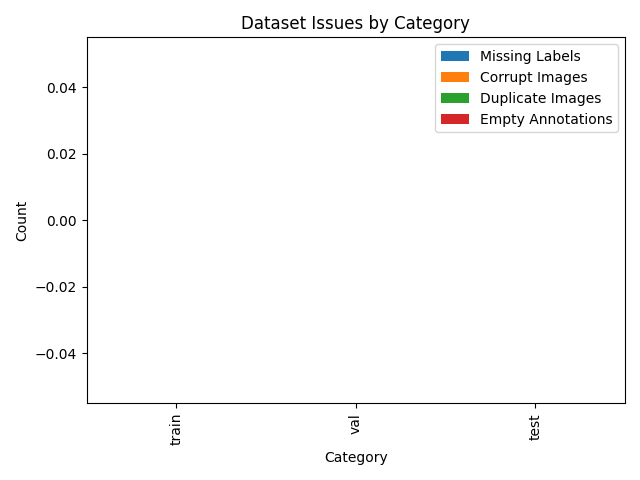
\includegraphics[width=13cm,height=11cm]{images/images/Visualization/data_cleaning_visualization.png}
    \caption{Data Cleaning Summary} 
    \label{fig:exploratory_cleaning_summary} 
\end{figure}


\subsection{Data Splitting and Visualization}
\begin{itemize}
  \item \textbf{Training data set (70\%):} Consisting of 1,890 images, this subset was used to train the model, enabling it to learn and recognize the patterns associated with fish species.

\item \textbf{Validation Dataset (15\%):} Consisting of 405 images, this subset was used to fine-tune the model's hyperparameters and monitor its performance during training to prevent overfitting.

\item \textbf{Testing Dataset (15\%):} Consisting of 405 images, this subset was reserved for evaluating the final model's performance on unseen data providing an unbiased generalization and assessment. 
\end{itemize}


The fish image dataset consists of 2,700 images, evenly distributed across 18 different fish species, with each species represented by 150 images.  Table~\ref{tab:species_distribution} shows the dataset distribution per species.


\vspace{0.5cm} % Adds vertical space

\begin{table}[H]
\centering
\caption{Dataset Distribution per Species}
\label{tab:species_distribution}
\begin{tabular}{|l|c|c|c|c|}
\hline
\textbf{Species} & \textbf{Total Images} & \textbf{Train} & \textbf{Validation} & \textbf{Test} \\
\hline
Tilapia & 150 & 105 & 23 & 22 \\
Molmol & 150 & 105 & 23 & 22 \\
Gutob & 150 & 105 & 23 & 22 \\
Bisugo & 150 & 105 & 23 & 22 \\
Bangus & 150 & 105 & 23 & 22 \\
Pulag-ikog & 150 & 105 & 23 & 22 \\
Tamban & 150 & 105 & 23 & 22 \\
Labahita & 150 & 105 & 23 & 22 \\
Danggit & 150 & 105 & 23 & 22 \\
Kitong & 150 & 105 & 23 & 22 \\
Anduhaw & 150 & 105 & 23 & 22 \\
Pompano & 150 & 105 & 23 & 22 \\
Sulid & 150 & 105 & 23 & 22 \\
Bilong-bilong & 150 & 105 & 23 & 22 \\
Barungoy & 150 & 105 & 23 & 22 \\
Budlisan & 150 & 105 & 23 & 22 \\
Talakitok & 150 & 105 & 23 & 22 \\
Maya-maya & 150 & 105 & 23 & 22 \\
\hline
\textbf{Total} & \textbf{2,700} & \textbf{1,890} & \textbf{414} & \textbf{396} \\
\hline
\end{tabular}
\end{table}

The dataset was then split into 70\% for training, 15.3\% for validation, and 14.7\% for testing. As a result, each fish species has 105 images for training, 23 for validation, and 22 for testing. Figure~\ref{fig:datasplit_distribution_across_species} and Figure~\ref{fig:datasplit_distribution_general} shown below illustrate the data split distribution for training, validation, and testing.


\begin{landscape}
\begin{figure}[p]
    \centering
    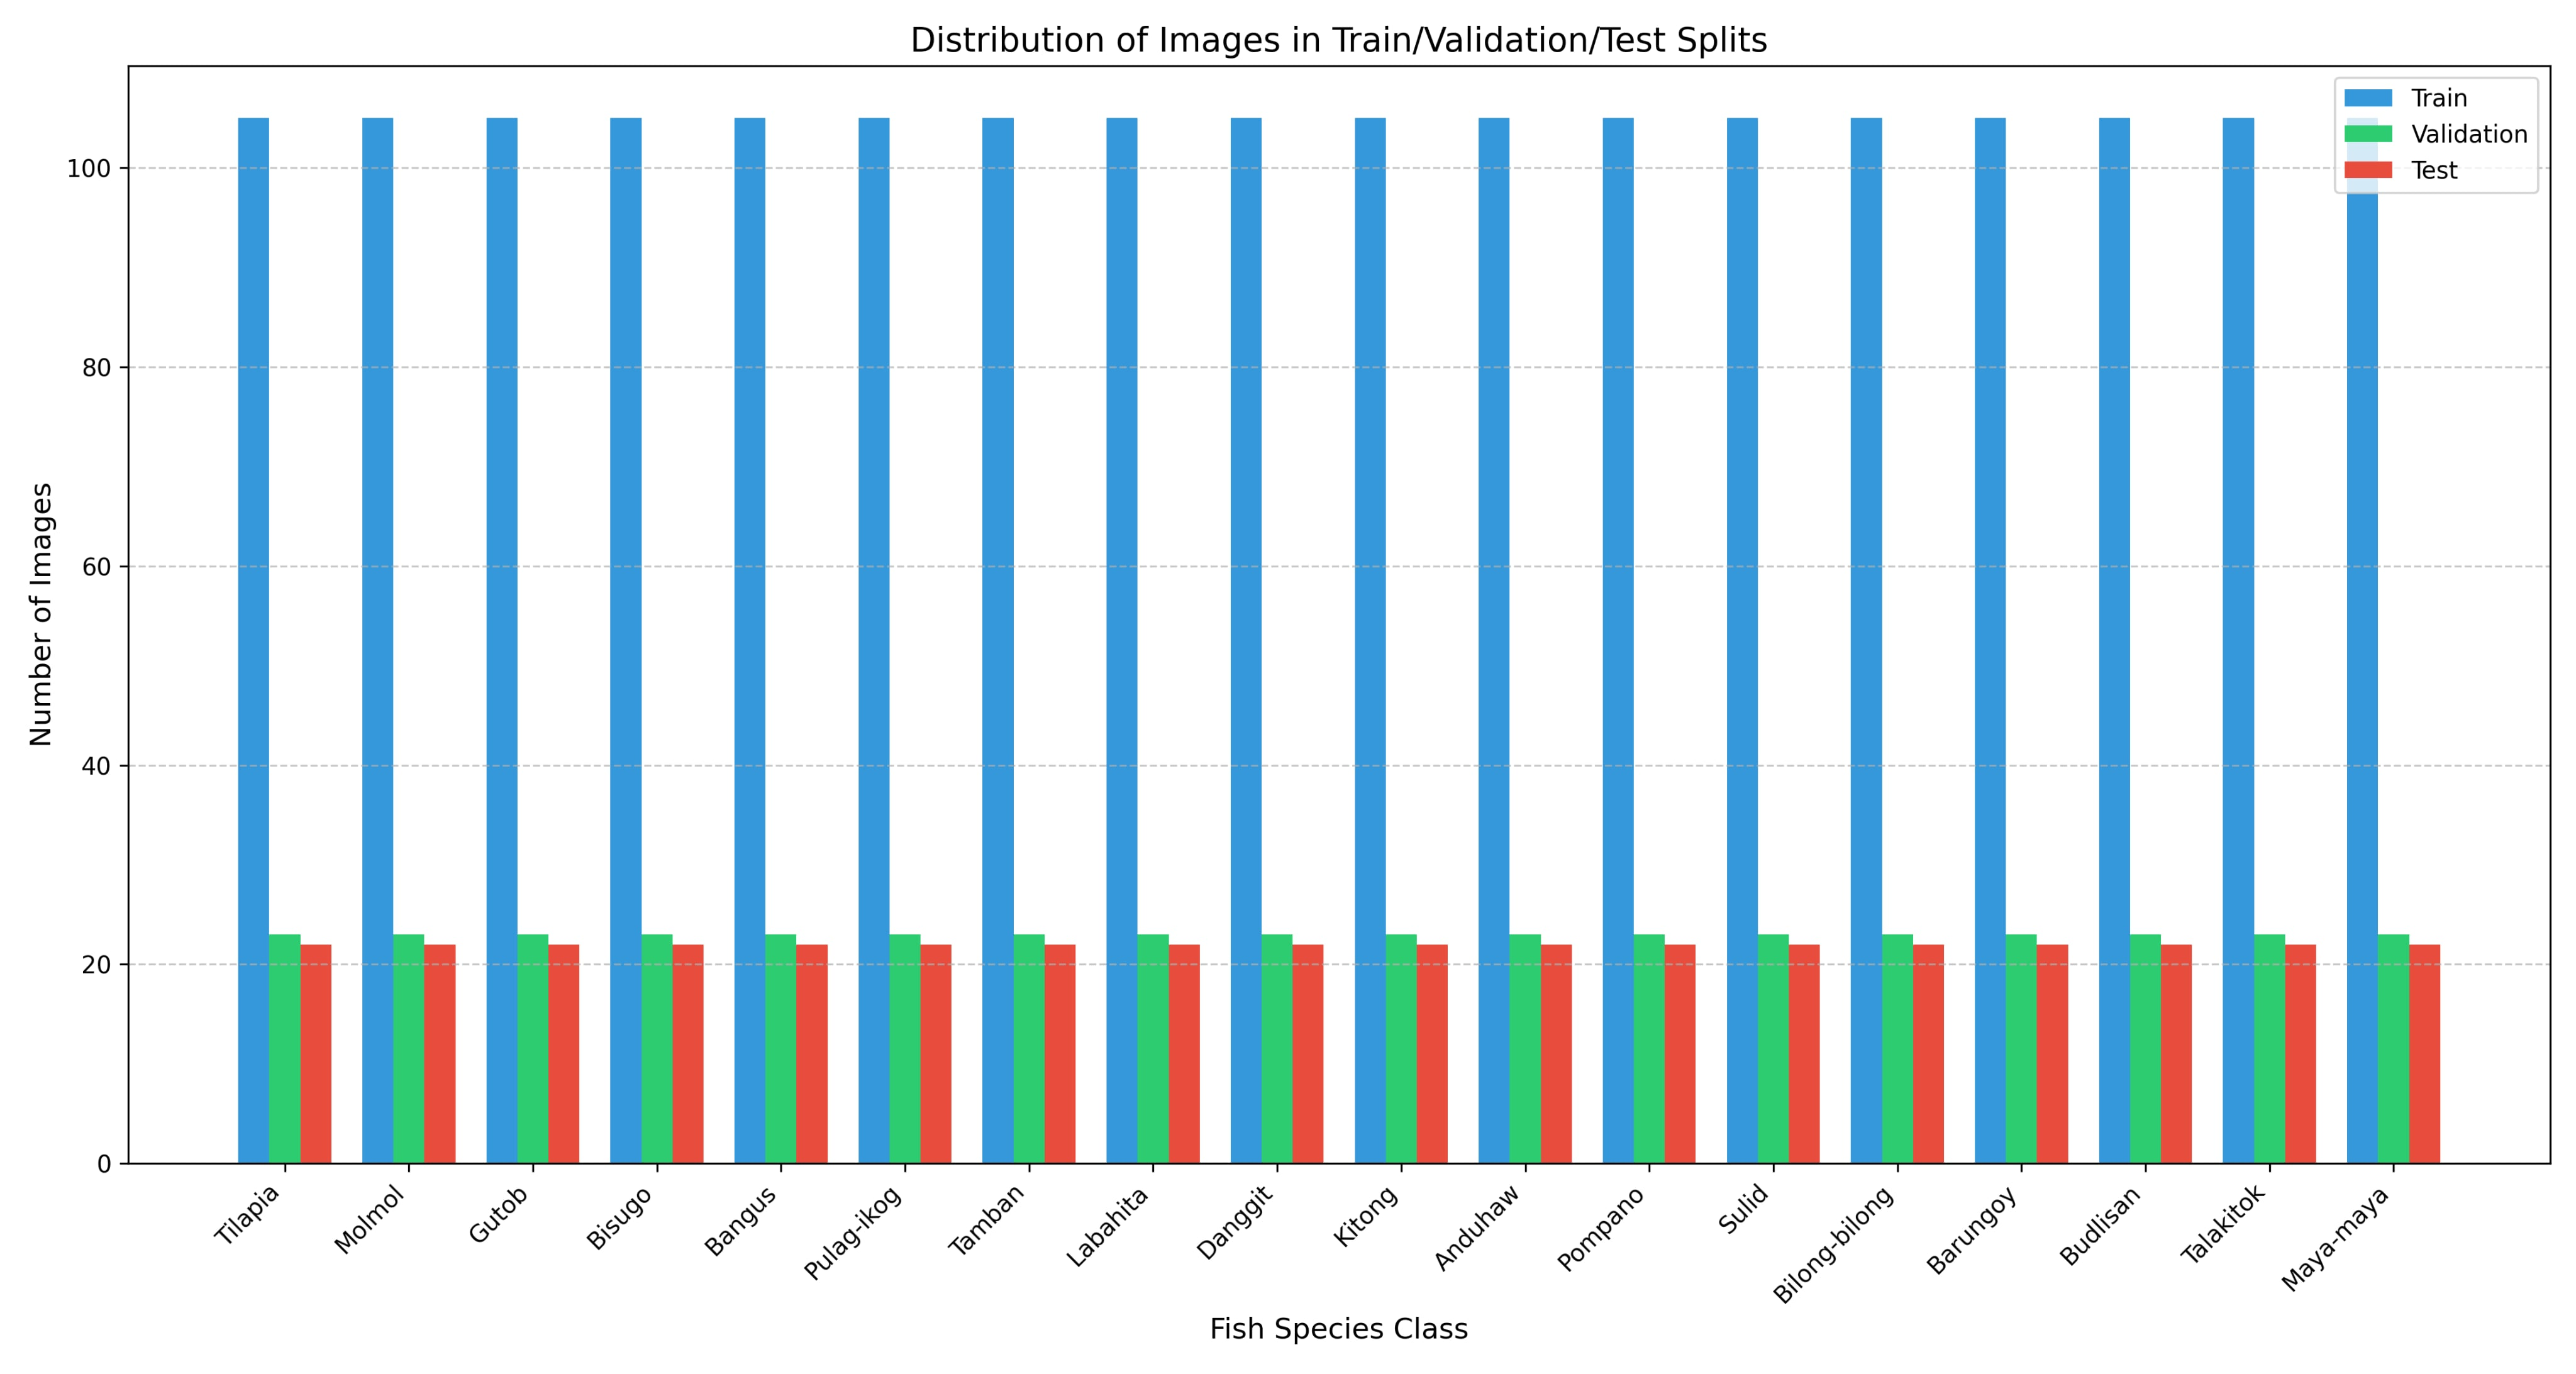
\includegraphics[height=0.80\textheight]{images/images/Visualization/datasplit_distribution_acrossFishSpecies.jpg}
    \caption{Data Split Distribution in Train, Validation and Testing}
    \label{fig:datasplit_distribution_across_species}
\end{figure}
\end{landscape}


\begin{figure}[H]
    \centering
    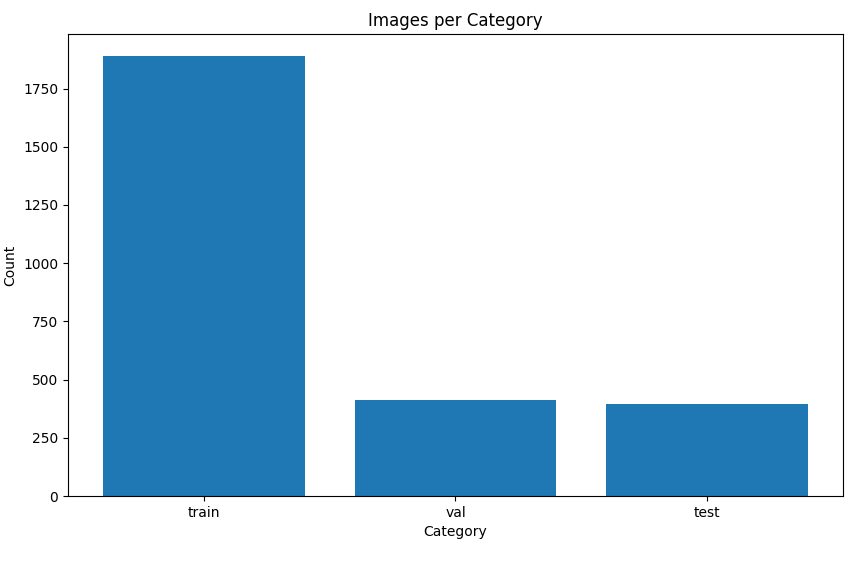
\includegraphics[width=13cm,height=11cm]{images/images/Visualization/images per category.png}
    \caption{Data Split Distribution} 
    \label{fig:datasplit_distribution_general}
\end{figure} 



\subsection{Data Augmentation}
To enhance the robustness and generalization capability of the YOLOv11 model, we applied four augmentation techniques to the training set using the Albumentations library. These transformations were designed to simulate real-world variations and help the model learn invariant features. The parameters used are described below, directly derived from the Python augmentation pipeline. The details of these augmentation techniques and their parameters are summarized in Table~\ref{tab:augmentation_techniques}

\newcolumntype{L}{>{\raggedright\arraybackslash}X}

\begin{table}[H]
\centering
\caption{Data Augmentation Technique Parameters}
\label{tab:augmentation_techniques}
\begin{tabularx}{\textwidth}{|L|L|L|}
\hline
\textbf{Augmentation} & \textbf{Description} & \textbf{Parameters Used} \\
\hline
Horizontal Flip (Hflip) & Flips the image horizontally. Simulates reversed fish orientations. & \texttt{p=1.0} (applied to all images) \\
\hline
Vertical Flip (Vflip) & Flips the image vertically. Captures vertical symmetry or varied capture angles. & \texttt{p=1.0} (applied to all images) \\
\hline
CLAHE (Contrast Limited Adaptive Histogram Equalization) & Enhances local contrast, especially useful for poorly lit fish images. & \texttt{clip\_limit=4.0}, \texttt{tile\_grid\_size=(8, 8)}, \texttt{p=1.0} \\
\hline
Hue-Saturation-Value Shift (HueSat) & Alters image colors to simulate varying lighting conditions (e.g., daylight, shadows). & \texttt{hue\_shift\_limit=±20}, \texttt{sat\_shift\_limit=±30}, \texttt{val\_shift\_limit=±20}, \texttt{p=1.0} \\
\hline
\end{tabularx}
\end{table}

From the initial 70\% training split comprising 1,890 raw images, a 4× augmentation strategy was applied using techniques such as horizontal flip, vertical flip, CLAHE, and hue-saturation-value shifts. This process generated 7,560 additional augmented images (1,890 × 4), bringing the total number of training images to 9,450 when the original and augmented images are combined.

\begin{table}[H]
\centering
\caption{Dataset Augmentation Statistics}
\label{tab:augmentation_stats}
\begin{tabular}{|l|c|c|c|}
\hline
\textbf{Dataset Split} & \textbf{Original Count} & \textbf{Augmented Count} & \textbf{Total Count} \\
\hline
Train & 1,890 & 7,560 & 9,450 \\
Validation & 414 & 0 & 414 \\
Test & 396 & 0 & 396 \\
\hline
\textbf{Total} & \textbf{2,700} & \textbf{7,560} & \textbf{10,260} \\
\hline
\end{tabular}
\end{table}


\begin{center}
\fbox{%
  \begin{minipage}{\textwidth}
    \begin{center}
        \begin{minipage}{0.19\textwidth}
            \centering
            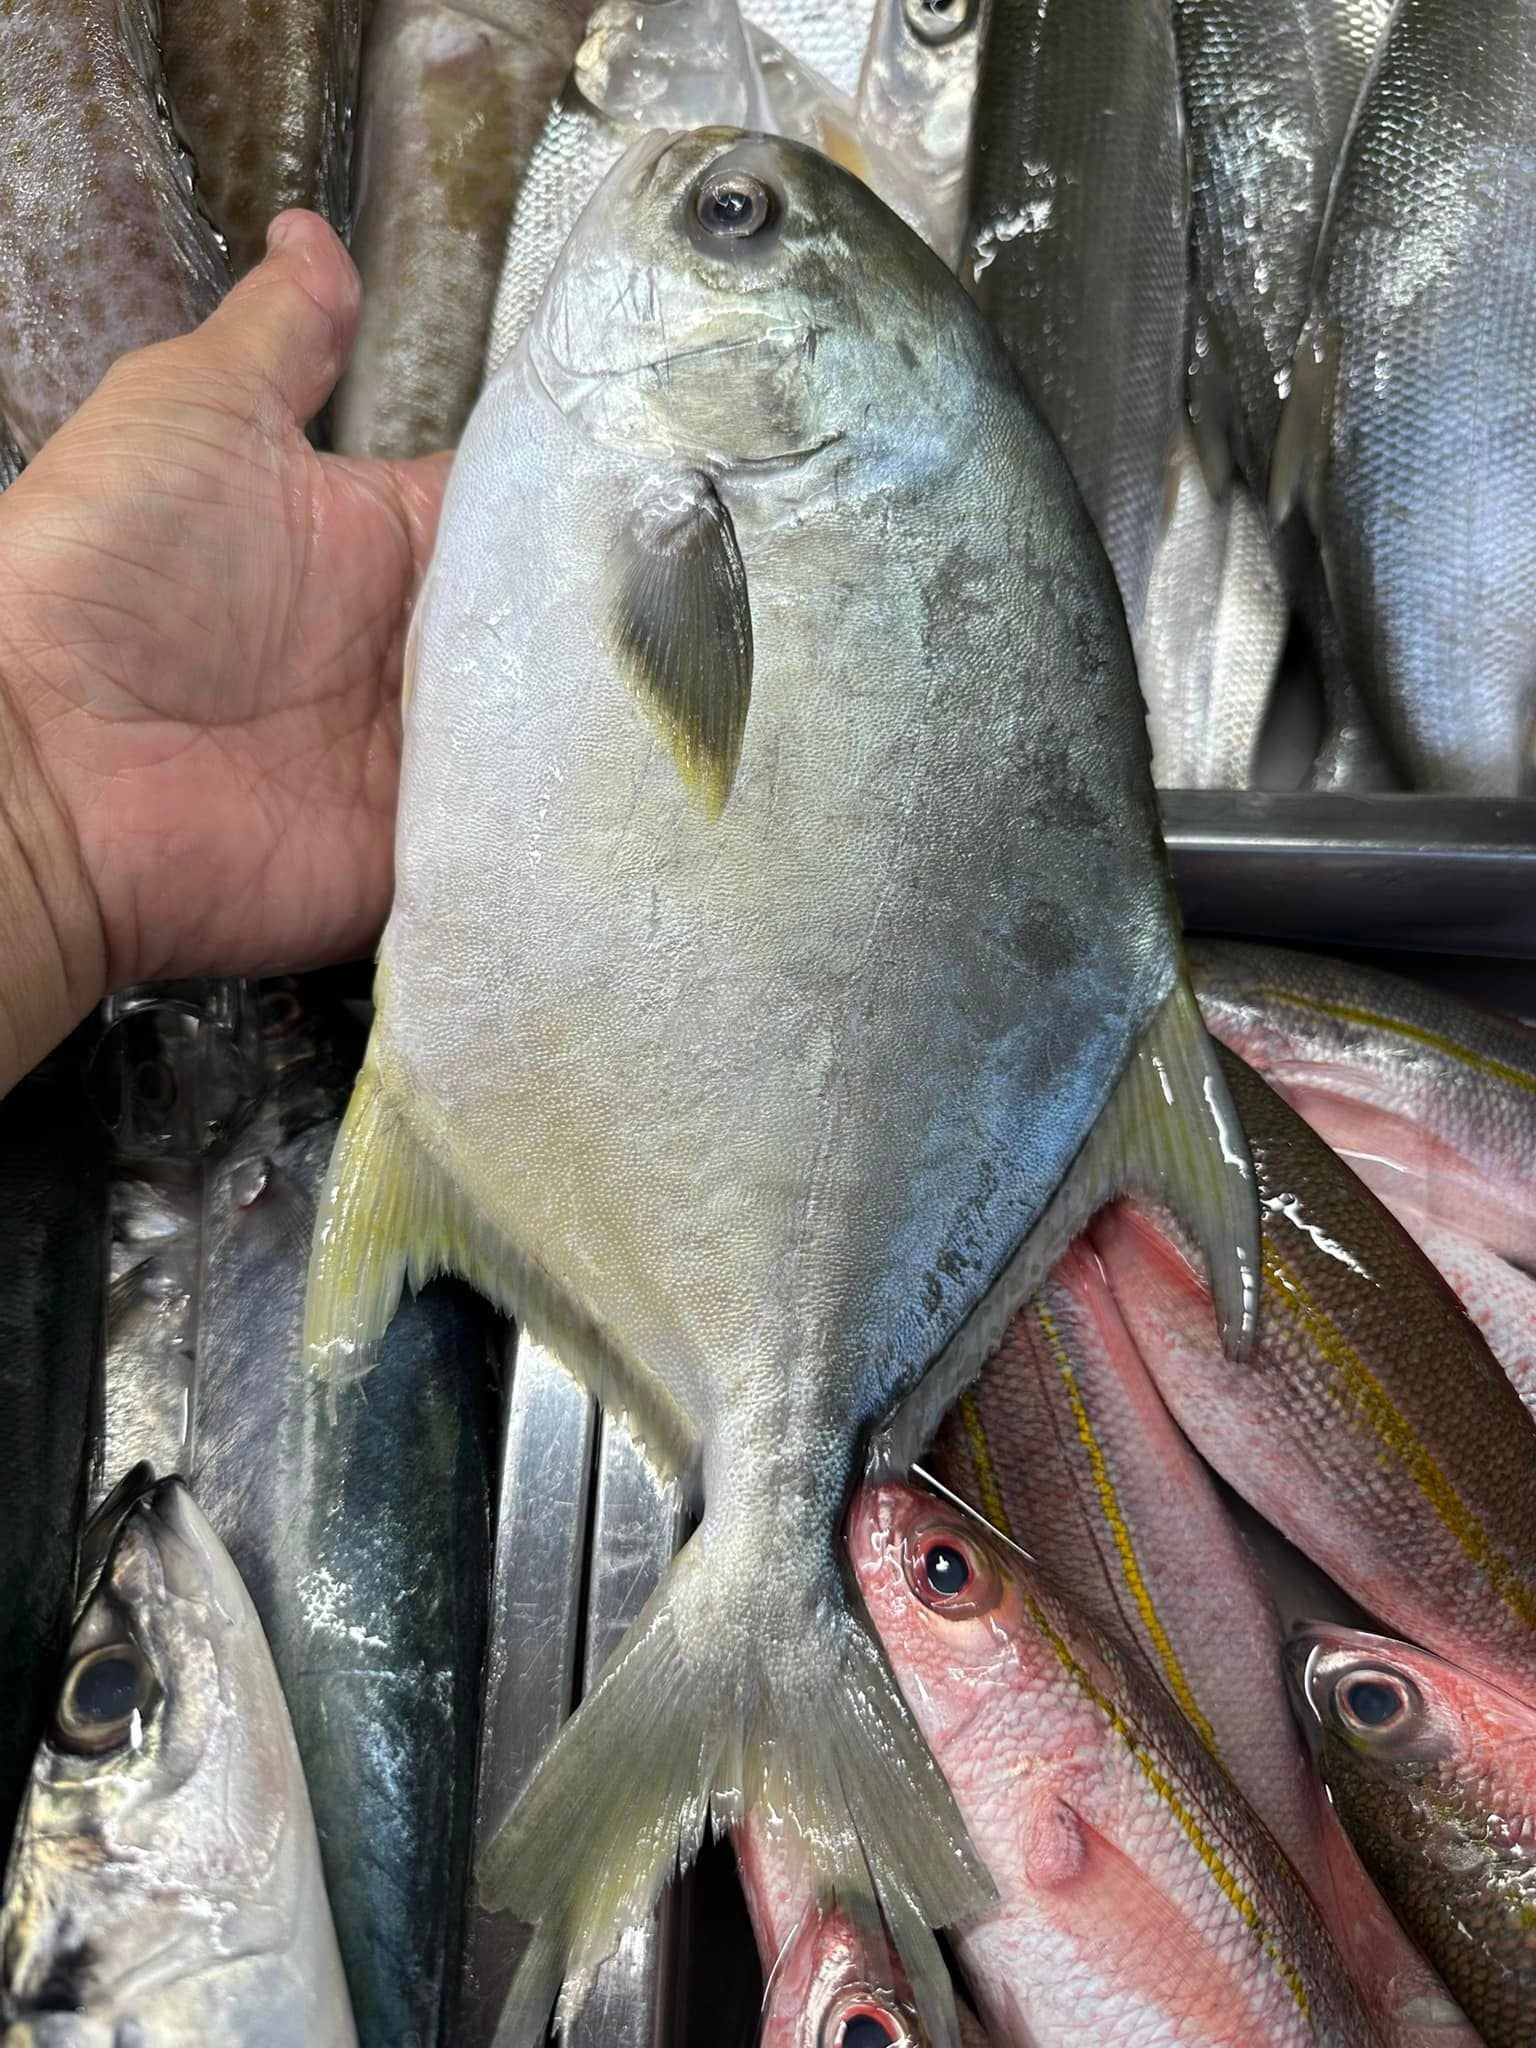
\includegraphics[width=\linewidth]{images/images/Visualization/original.jpg}
            
            {\footnotesize Original Image}
        \end{minipage}
        \hfill
        \begin{minipage}{0.19\textwidth}
            \centering
            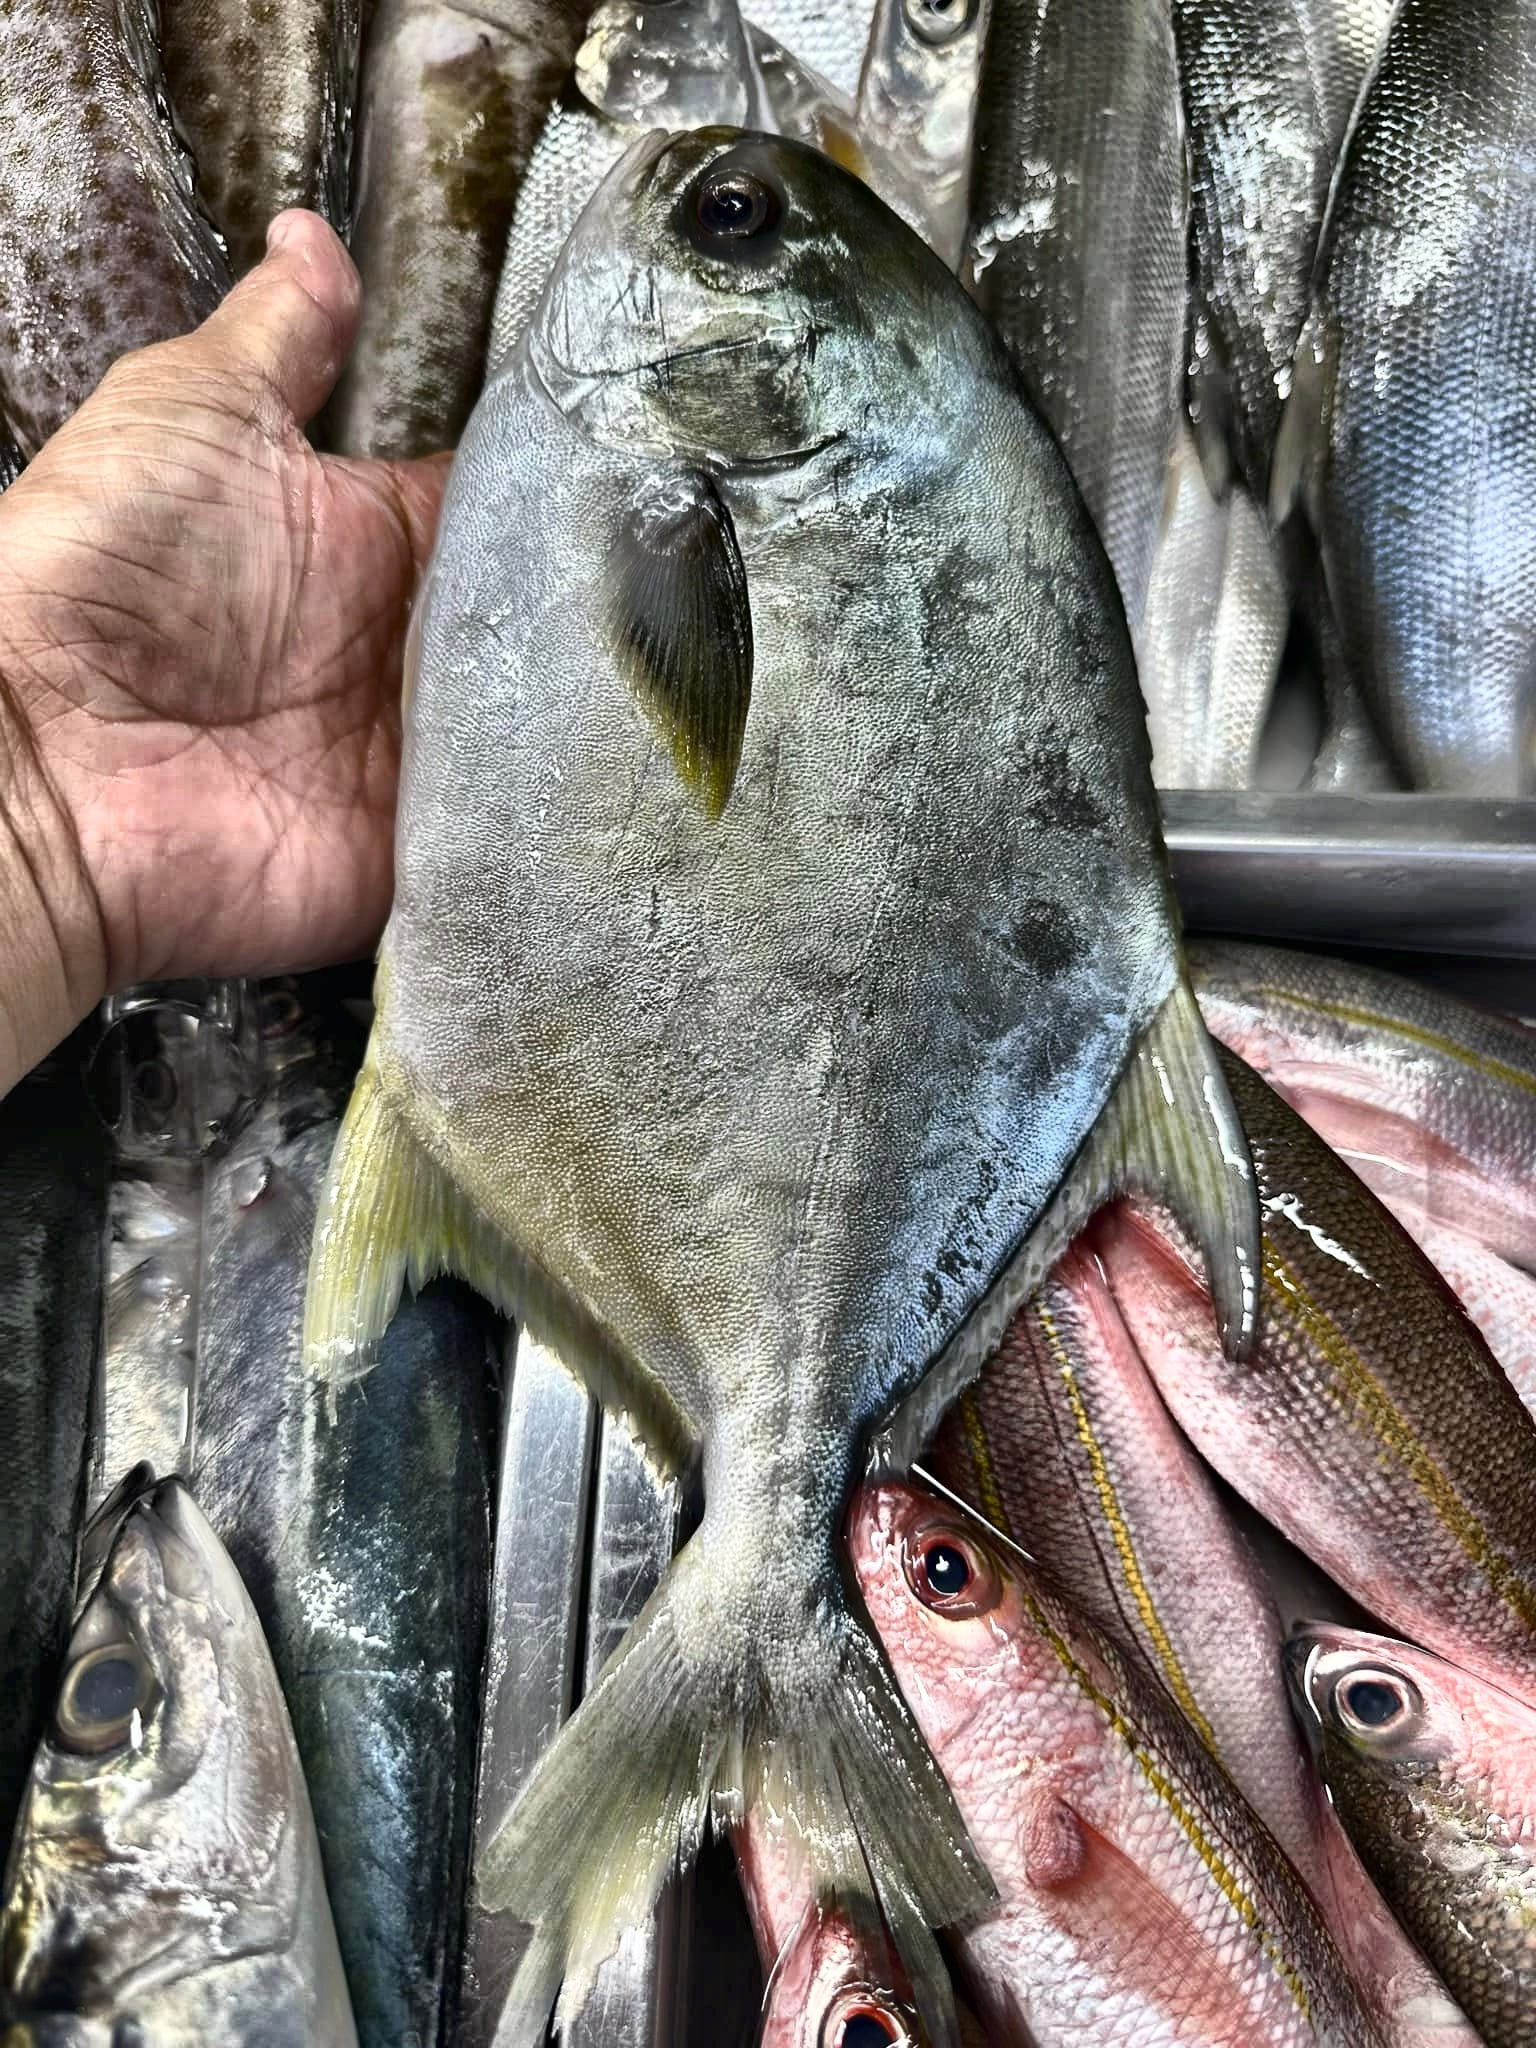
\includegraphics[width=\linewidth]{images/images/Visualization/CLAHE.jpg}
            
            {\footnotesize CLAHE}
        \end{minipage}
        \hfill
        \begin{minipage}{0.19\textwidth}
            \centering
            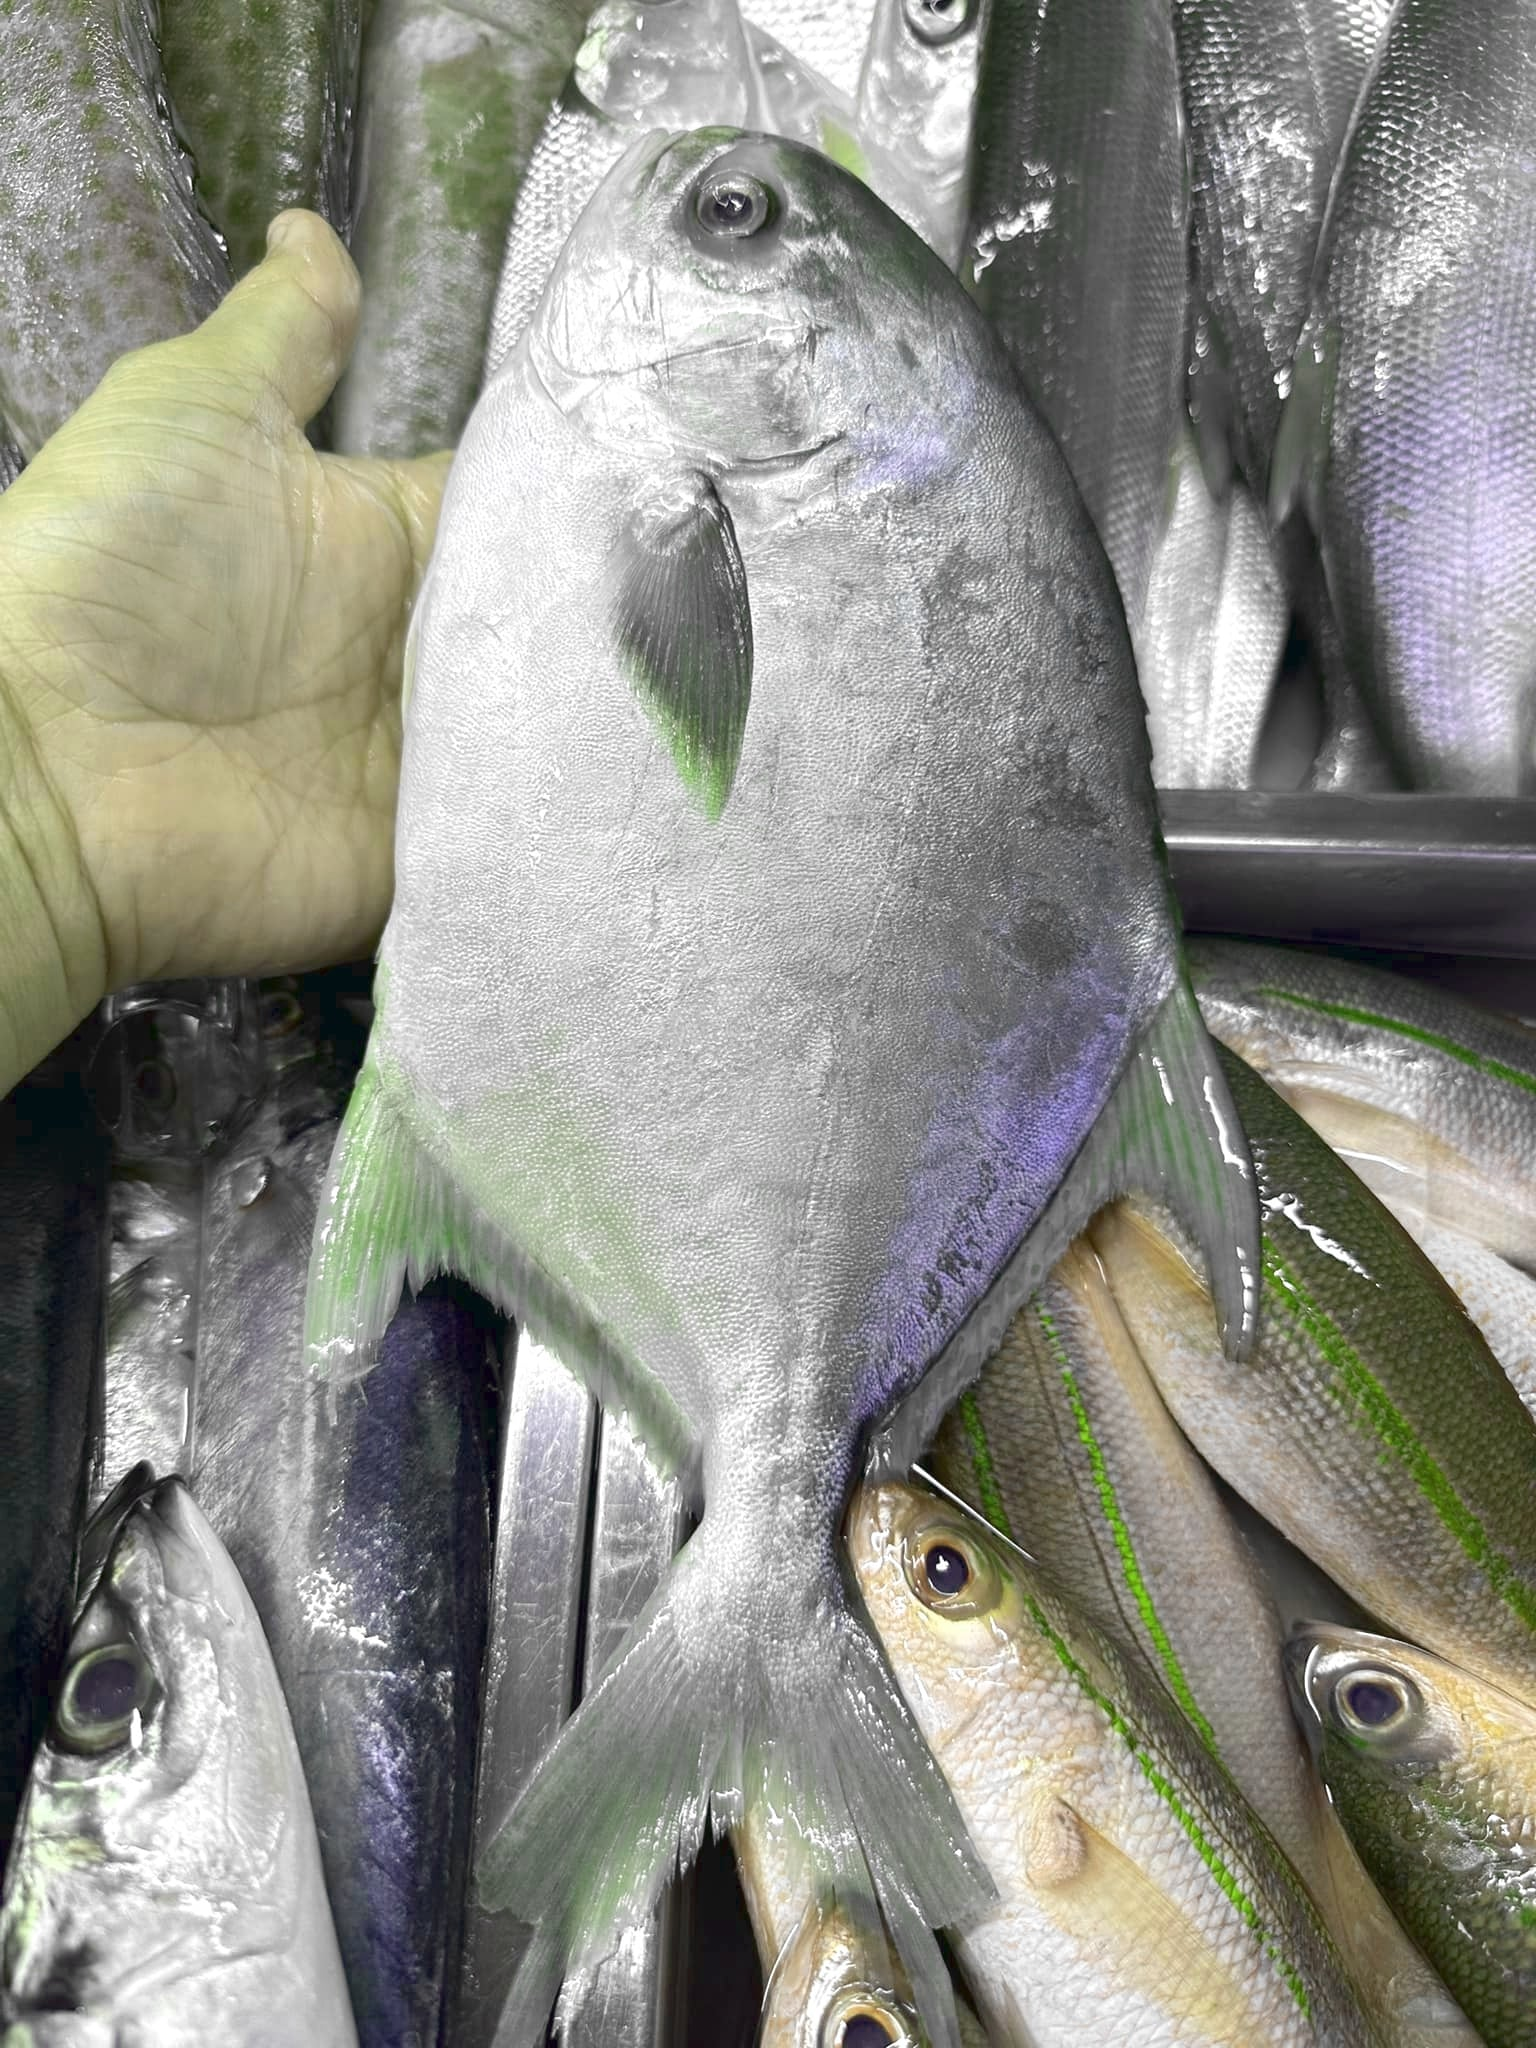
\includegraphics[width=\linewidth]{images/images/Visualization/huesat.jpg}
            
            {\footnotesize Hue Saturation}
        \end{minipage}
        \hfill
        \begin{minipage}{0.19\textwidth}
            \centering
            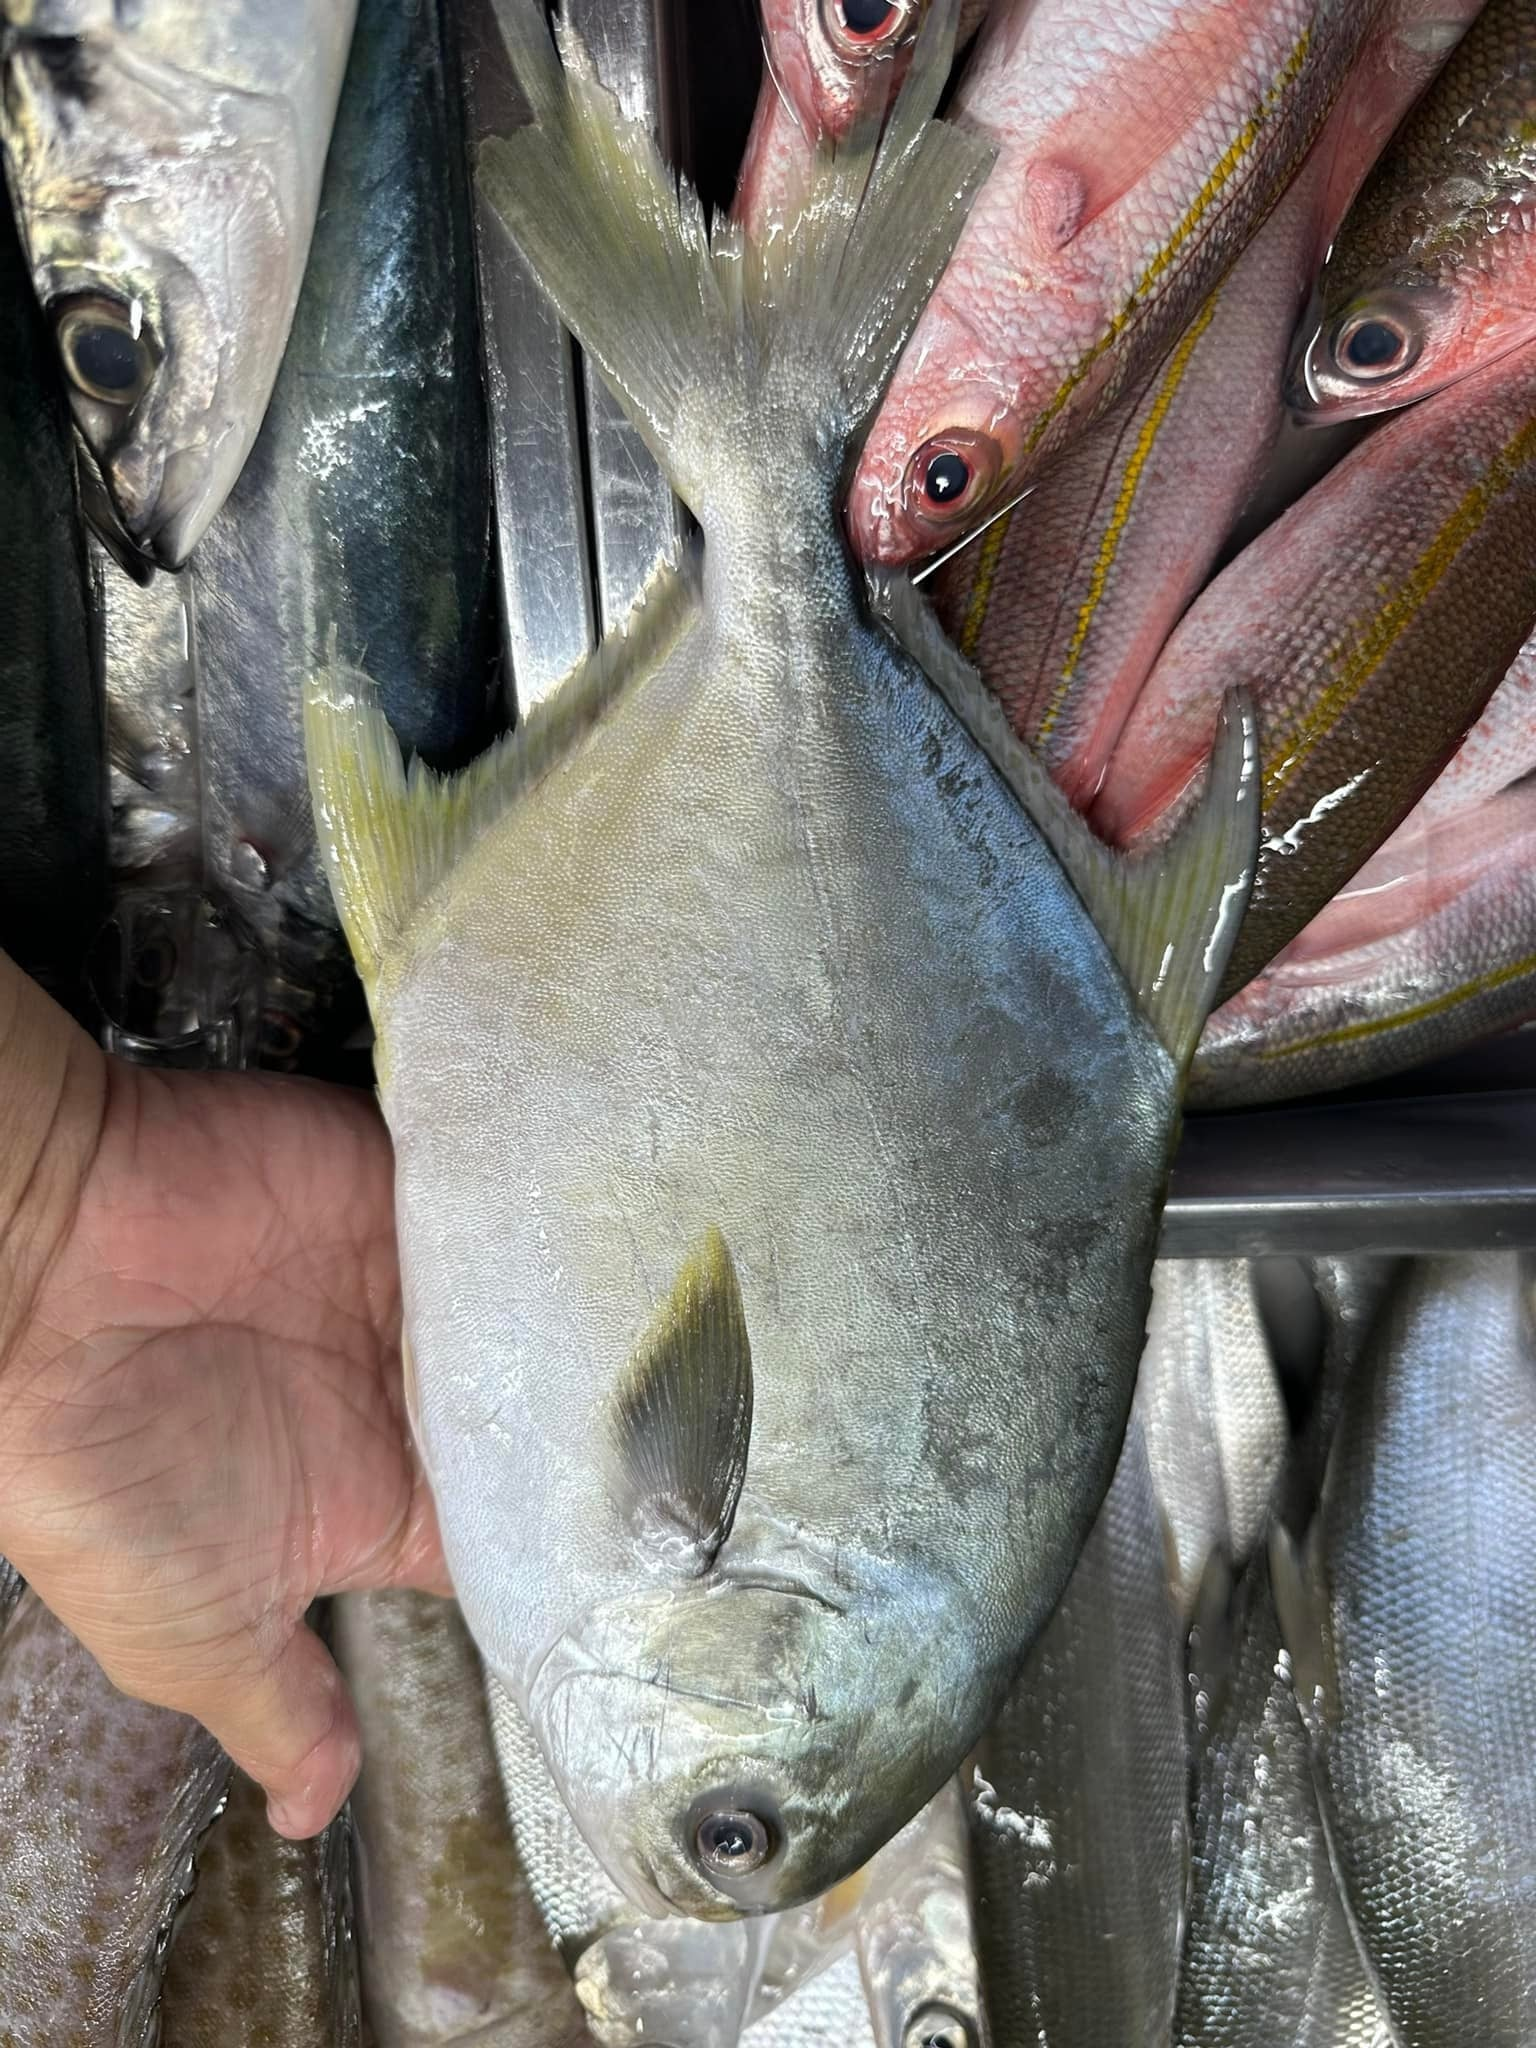
\includegraphics[width=\linewidth]{images/images/Visualization/vertical.jpg}
            
            {\footnotesize Vertical Flip}
        \end{minipage}
        \hfill
        \begin{minipage}{0.19\textwidth}
            \centering
            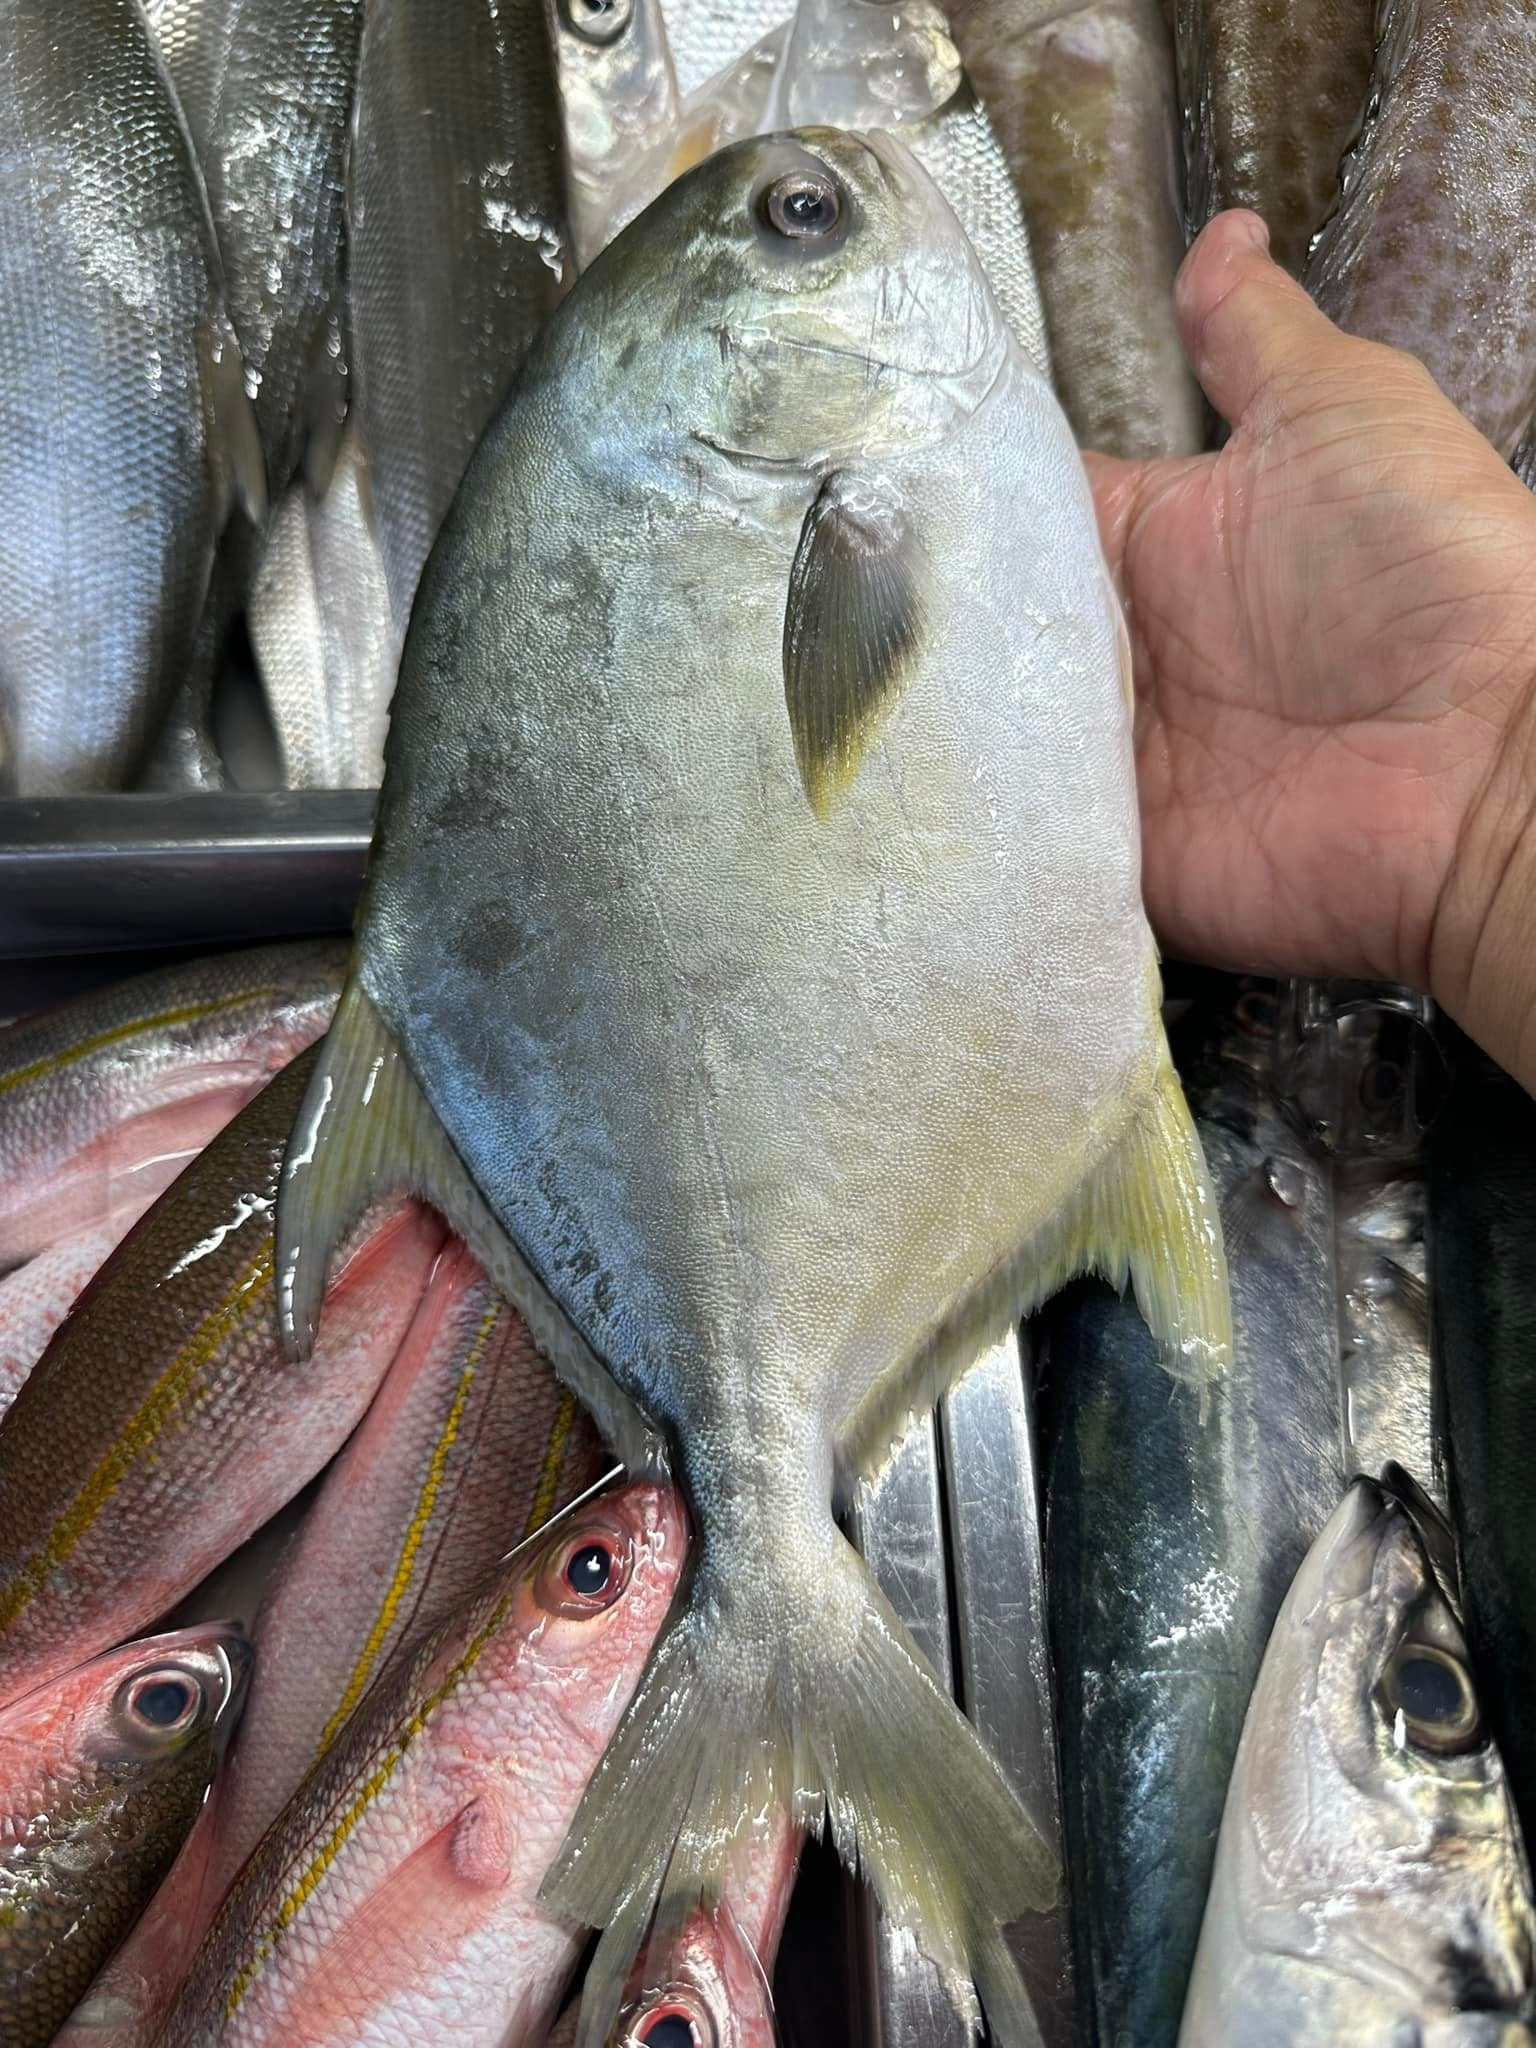
\includegraphics[width=\linewidth]{images/images/Visualization/horizontal.jpg}
            
            {\footnotesize Horizontal Flip}
        \end{minipage}
    \end{center}
  \end{minipage}%
}
\vspace{0.75em}

\captionof{figure}{Augmentation Techniques Applied on an Original Fish Image}
\label{fig:augmentation_samples}
\end{center}

Table~\ref{tab:augmentation_stats} shows the breakdown of the original dataset and its expansion after applying data augmentation. The original dataset contained 2,700 images across three splits. Figure~\ref{fig:augmentation_samples} illustrates the four augmentation techniques—horizontal flip, brightness-contrast adjustment, hue-saturation shift, and CLAHE (Contrast Limited Adaptive Histogram Equalization)—resulting in four new variants per image. Including the original, this brings the total to five versions per image. This augmentation strategy improves model robustness by exposing it to a broader range of visual conditions.

\section{Modelling}

This chapter presents the results gathered during the development and testing phases. It discusses the outcomes of the model's training, validation, and testing, as well as the system’s ability to correctly classify various fish species using object detection. The algorithm shown below illustrates the YOLOv11 training process along with the configured hyperparameters used during model training.


\begin{algorithm}
\caption{YOLOv11 Model Training Procedure}\label{alg:train_yolo}
\begin{algorithmic}[1]
\State \textbf{Input:} Dataset directory \texttt{dataset\_path}, pretrained weights \texttt{yolov11m.pt}, configuration file \texttt{data.yaml}
\Statex
\State Initialize dataset path: \texttt{dataset\_path}
\State Load data configuration file: \texttt{data\_yaml} $\gets$ \texttt{dataset\_path}/\texttt{data.yaml}
\State Load pretrained model weights: \texttt{model\_path} $\gets$ \texttt{dataset\_path}/\texttt{yolo11m.pt}
\State Load model: \texttt{model} $\gets$ \texttt{YOLO(model\_path)}
\Statex
\State Define training parameters:
\State \quad \texttt{data} $\gets$ \texttt{data\_yaml}
\State \quad \texttt{epochs} $\gets$ 40
\State \quad \texttt{imgsz} $\gets$ 640
\State \quad \texttt{batch} $\gets$ 2
\State \quad \texttt{device} $\gets$ \texttt{'cuda'}
\State \quad \texttt{project} $\gets$ \texttt{"runs"}
\State \quad \texttt{name} $\gets$ \texttt{"results"}
\State \quad \texttt{workers} $\gets$ 0
\Statex
\State Train the YOLOv11 model using the specified parameters
\State Store training results in the designated project directory
\State Return trained model and performance logs
\end{algorithmic}
\end{algorithm}


\begin{table}[H]
    \makebox[\textwidth][c]{% 
        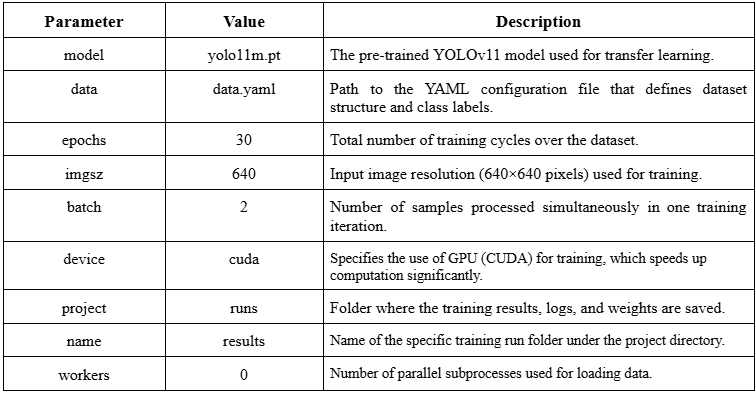
\includegraphics[width=1.05\textwidth]{images/images/table_description_yolo_import.png}%
    }
    \caption{Model Configuration and Training Parameters}
    \label{tab:table_description_yolo_import}
\end{table}

The table~\ref{tab:table_description_yolo_import} outlines the training configuration used for fine-tuning the YOLOv11 model. The model was initialized with the \texttt{yolov11m.pt} weights and trained on a custom dataset located in the specified directory. The training was performed using a small batch size of 2 to accommodate GPU memory limitations. The input images were resized to 640×640 pixels, and training was run for 30 epochs. The \texttt{cuda} device ensured that GPU acceleration was leveraged to reduce training time. The results were stored in the \texttt{runs} project folder under the run name \texttt{result}.

\subsection{Quantitative Metrics}
Figure~\ref{tab:val_overall_metrics} presents the quantitative metrics obtained after the training and validation phases, providing a comprehensive overview of the model’s performance. These metrics include key evaluation indicators such as precision, recall, F1-Score, and mean average precision (mAP), which are essential in assessing the accuracy and reliability of the YOLOv11 model in detecting and classifying fish species.


\begin{figure}[H]
    \centering
    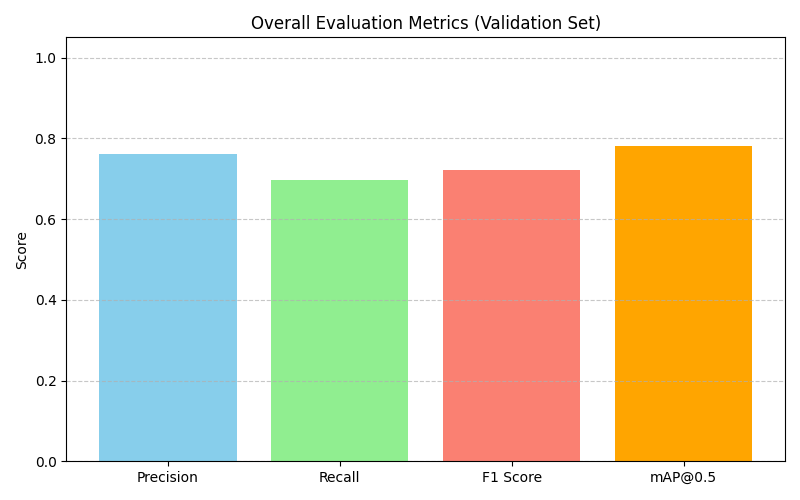
\includegraphics[width=1.0\textwidth]{images/images/Trained/results_visualization/val_overall_metrics.png}
    \caption{Overall Evaluation Metrics.}
    \label{tab:val_overall_metrics}
\end{figure}

 The model's performance on key metrics:
\begin{itemize}
    \item \textbf{Precision:} 0.76
    \item \textbf{Recall:} 0.69
    \item \textbf{F1-Score:} 0.72
    \item \textbf{mAP@0.5:} 0.78
\end{itemize}

The high mAP@0.5 indicates the model is effective at identifying and localizing objects at a standard intersection-over-union threshold.

\begin{figure}[H]
    \centering
    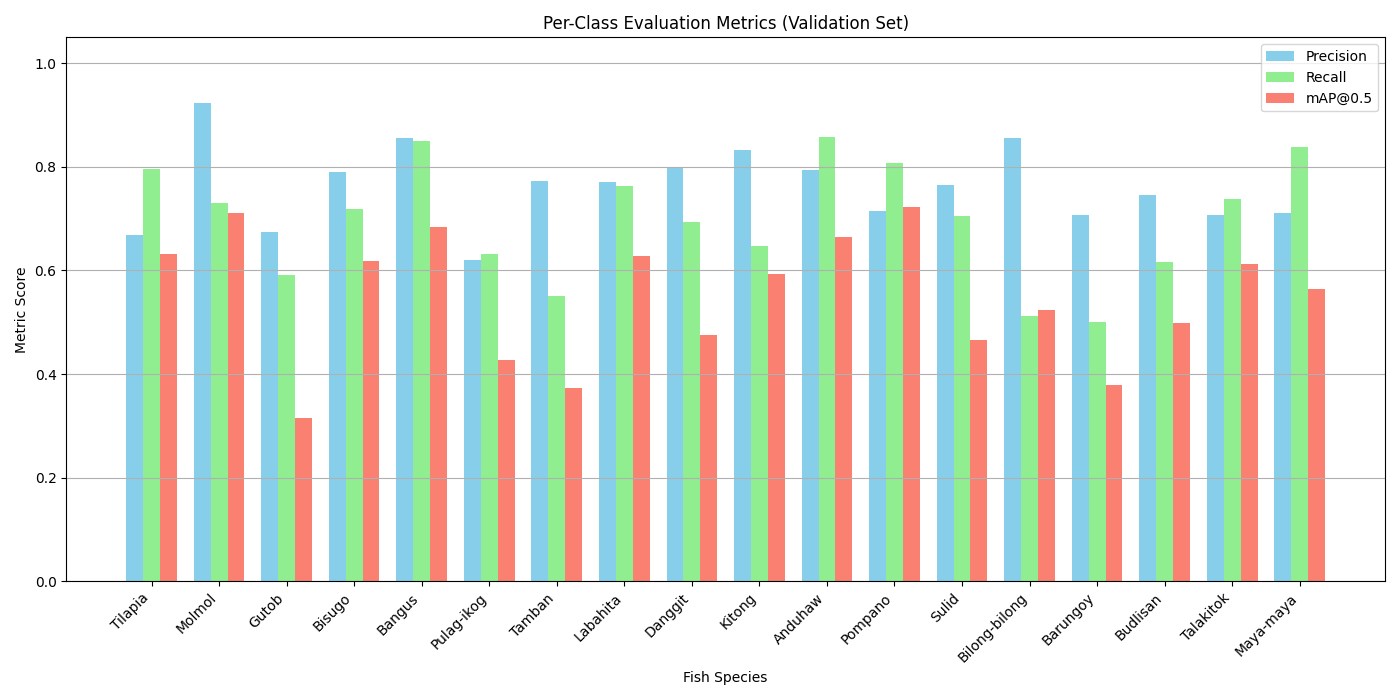
\includegraphics[width=1.0 \textwidth]{images/images/Trained/results_visualization/val_per_class_metrics.png}
        \caption{Per-class Evaluation Metrics}
    \label{tab:val_per_class_metrics}
\end{figure}
Figure~\ref{tab:val_per_class_metrics} presents the detailed performance metrics for each fish species class immediately following the training phase. The metrics include precision, recall, F1-score, and support, allowing for a granular assessment of how well the model has learned to detect and classify each species based on the training data. The visualization highlights any class imbalances or model biases that may need further tuning before final evaluation.
\begin{figure}[H]
    \makebox[\textwidth][c]{%
        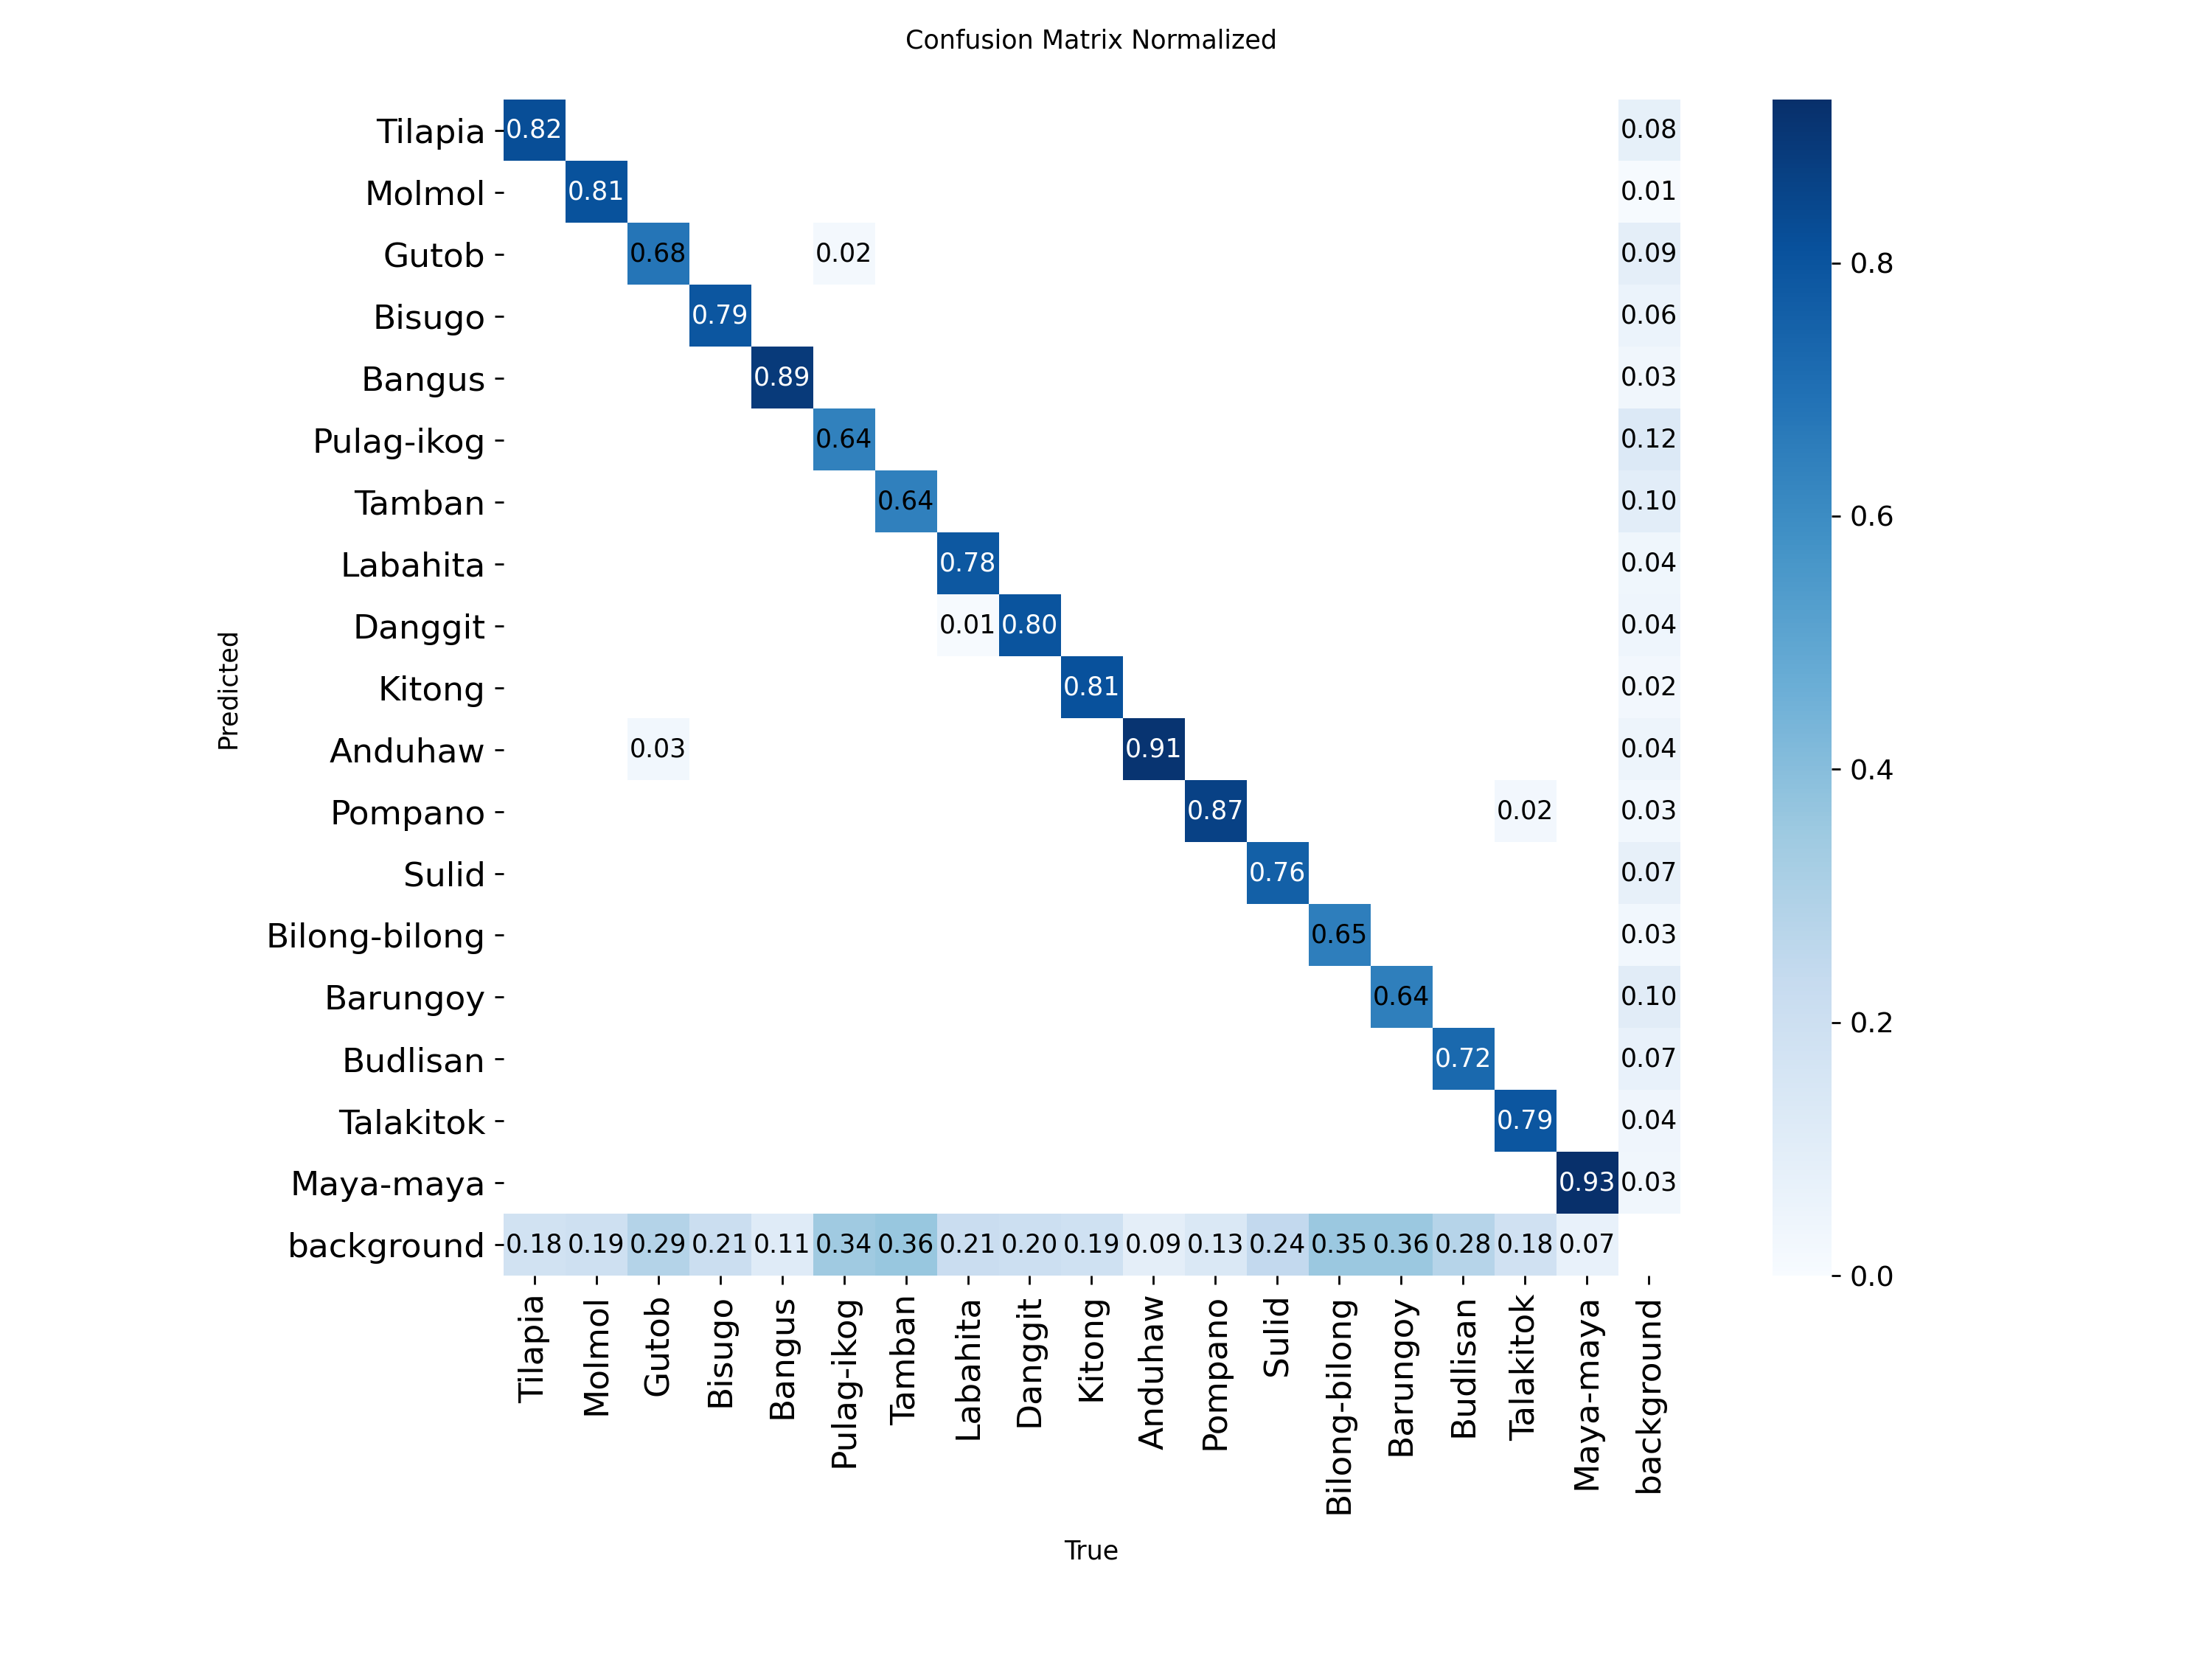
\includegraphics[width=1.5\textwidth]{images/images/Trained/results_visualization/confusion_matrix_normalized.png}%
    }
    \caption{Confusion Matrix Normalized}
    \label{tab:confusion_matrix_normalized}
\end{figure}

The Figure~\ref{tab:confusion_matrix_normalized} is the normalized confusion matrix reveals the model’s classification consistency across different species. High classification accuracy is seen for \textit{Bangus} (0.89), \textit{Pompano} (0.87), and \textit{Maya-maya} (0.93). In contrast, species such as \textit{Pulag-ikog} and \textit{Tamban} scored lower (0.64), indicating challenges in distinguishing them from other classes.

\section{Model Evaluation and Performance}

The evaluation of the trained YOLOv11m model was conducted using various quantitative and qualitative metrics to assess its performance on detecting and classifying multiple fish species. This subsection presents visualizations and numerical summaries such as class-wise metrics, loss trends, confusion matrix, and mAP values. These outputs provide insight into the model’s learning behavior during training, its accuracy on unseen validation data, and the overall reliability of its predictions in real-world scenarios.

\subsection{Quantitative Metrics}
 Figure~\ref{tab:test_overall_metrics}, shown below, presents the quantitative metrics obtained from the testing set, offering a detailed evaluation of the YOLOv11 model’s performance on unseen data. 
 
\begin{figure}[H]
    \centering
    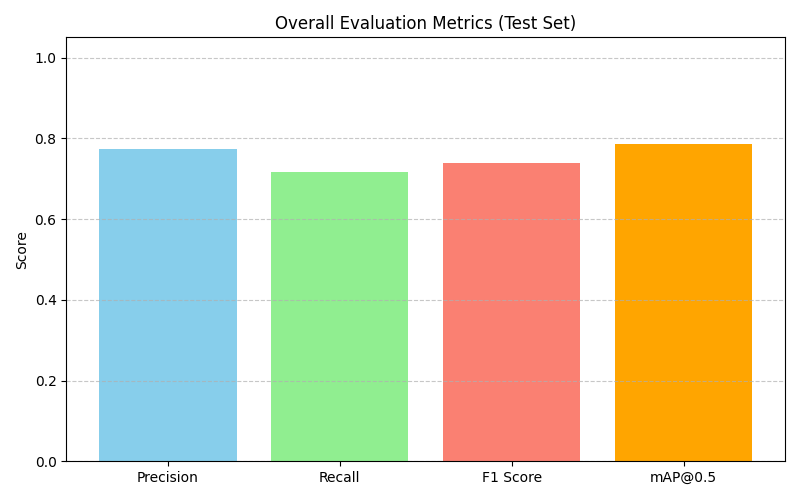
\includegraphics[width=1.0\textwidth]{images/images/Trained/results_visualization/test_overall_metrics.png}
    \caption{Overall Evaluation Metrics.}
    \label{tab:test_overall_metrics}
\end{figure}

 The model's performance on key metrics:
\begin{itemize}
    \item \textbf{Precision:} 0.78
    \item \textbf{Recall:} 0.72
    \item \textbf{F1-Score:} 0.74
    \item \textbf{mAP@0.5:} 0.79
\end{itemize}

\begin{table}[H]
\centering
\caption{Per-Class Image-Level Evaluation Statistics}
\begin{tabular}{|l|c|c|c|c|p{4cm}|}
\hline
\textbf{Fish Species} & \textbf{Total Test} & \textbf{Correct} & \textbf{Misclassified} & \textbf{Accuracy} & \textbf{Common Mislabels} \\
\hline
Tilapia        & 22 & 22 & 0 & 100.00 & --- \\
Molmol         & 22 & 19 & 3 & 86.36 & None \\
Gutob          & 22 & 22 & 0 & 100.00 & --- \\
Bisugo         & 22 & 21 & 1 & 95.45 & None \\
Bangus         & 22 & 19 & 3 & 86.36 & None \\
Pulag-ikog     & 22 & 20 & 2 & 90.91 & None \\
Tamban         & 22 & 20 & 2 & 90.91 & None \\
Labahita       & 22 & 22 & 0 & 100.00 & --- \\
Danggit        & 22 & 21 & 1 & 95.45 & None \\
Kitong         & 22 & 21 & 1 & 95.45 & None \\
Anduhaw        & 22 & 16 & 6 & 72.73 & None, Gutob \\
Pompano        & 22 & 22 & 0 & 100.00 & --- \\
Sulid          & 22 & 21 & 1 & 95.45 & None \\
Bilong-bilong  & 22 & 21 & 1 & 95.45 & None \\
Barungoy       & 22 & 21 & 1 & 95.45 & None \\
Budlisan       & 22 & 21 & 1 & 95.45 & None \\
Talakitok      & 22 & 21 & 1 & 95.45 & Gutob \\
Maya-maya      & 22 & 20 & 2 & 90.91 & None \\
\hline
\end{tabular}
\label{tab:per-class-eval}
\end{table}

 Table~\ref{tab:per-class-eval} presents the per-class image-level evaluation statistics of the ClassiFish model across 18 fish species, with each class tested on 22 images. The model achieved perfect accuracy (100\%) for Tilapia, Gutob, Labahita, and Pompano, while several species such as Bisugo, Danggit, Kitong, Sulid, Bilong-bilong, Barungoy, Budlisan, and Talakitok reached high accuracy at 95.45\% with only one misclassification each. Pulag-ikog, Tamban, and Maya-maya followed closely with 90.91\% accuracy, each having two misclassifications. Molmol and Bangus both recorded 86.36\% accuracy due to three misclassified images. The lowest accuracy was observed in the Anduhaw class at 72.73\%, with six misclassifications, commonly confused with Gutob. The “Common Mislabels” column reveals which species were frequently mistaken for others, though most classes exhibited minimal to no confusion, indicating strong class separability in the model’s predictions.

\begin{figure}[H]
    \centering
    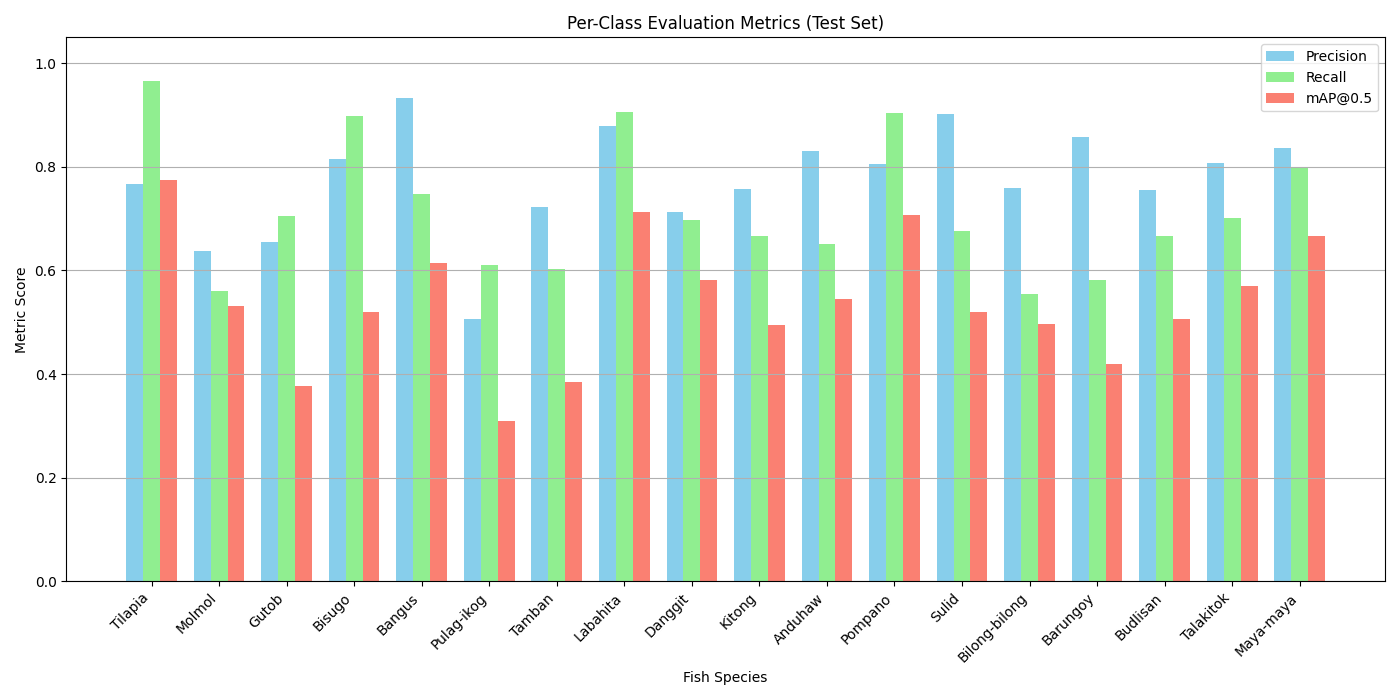
\includegraphics[width=1.0 \textwidth]{images/images/Trained/results_visualization/test_per_class_metrics.png}
        \caption{Per-class Evaluation Metrics}
    \label{tab:per_class_metrics}
\end{figure}
Figure~\ref{tab:per_class_metrics} shows the per-class performance metrics derived from evaluating the trained model on the unseen test dataset. It includes precision, recall, F1-score, and support for each fish species, providing an objective measure of the model's generalization capability and robustness. Differences in metric values compared to the training evaluation help identify species that the model struggles to recognize accurately under real-world conditions.

\begin{figure}[H]
    \centering
    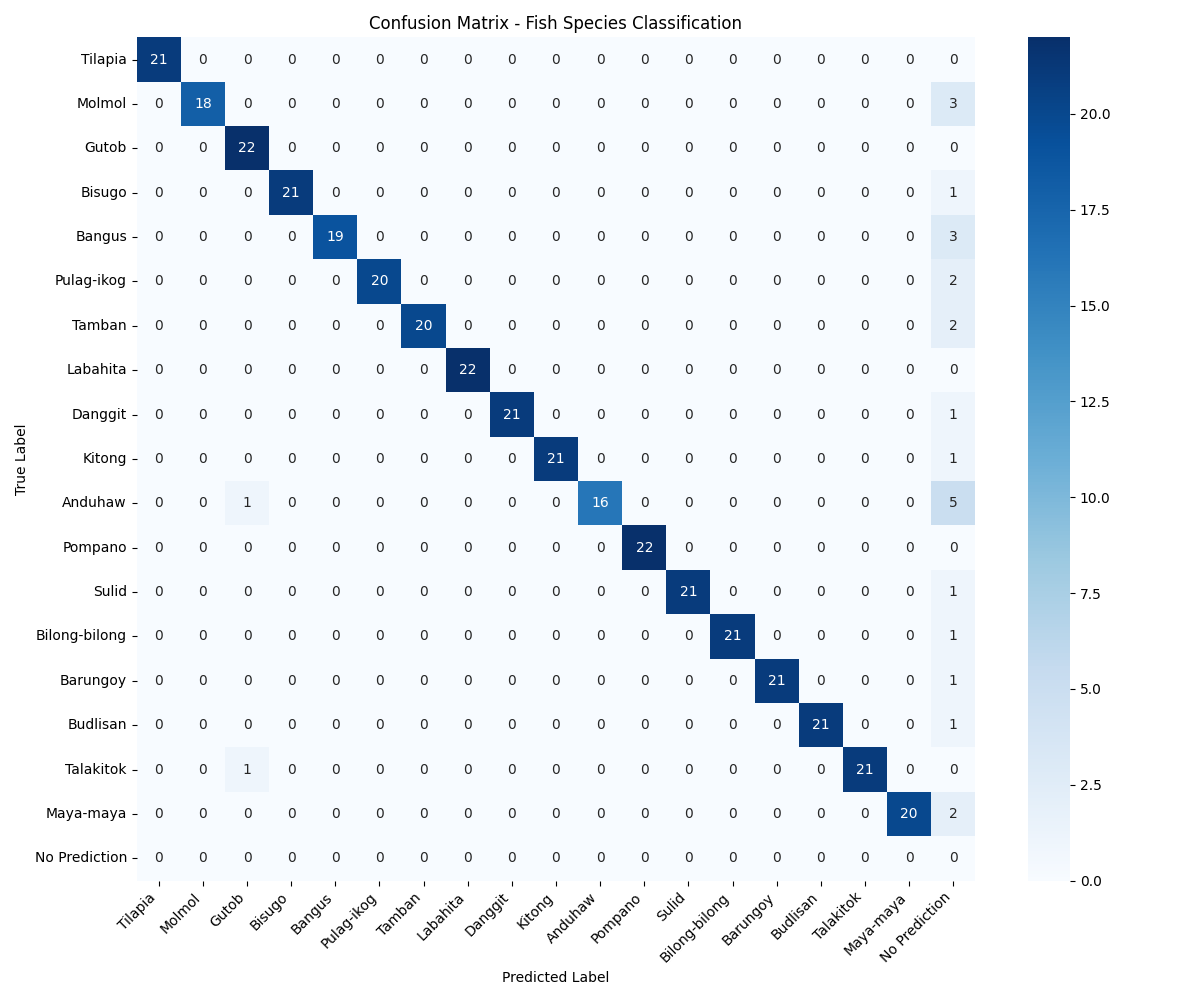
\includegraphics[width=1.0 \textwidth]{images/images/Trained/results_visualization/test_confusion_matrix.png}
        \caption{Per-class Evaluation Metrics}
    \label{tab:test_confusion_matrix}
\end{figure}


Figure~\ref{tab:test_confusion_matrix} shows that the model correctly predicted most samples for each fish species, with values mostly aligned along the diagonal. Each class generally has around 20 to 22 correct predictions, indicating consistent performance across categories. A few species, such as \textit{Anduhaw} and \textit{Molmol}, have some misclassifications or unpredicted cases. Overall, the model performs consistently, with a small number of errors in certain classes.


\begin{figure}[H]
    \centering
    \begin{minipage}{0.8\textwidth}
        \centering
        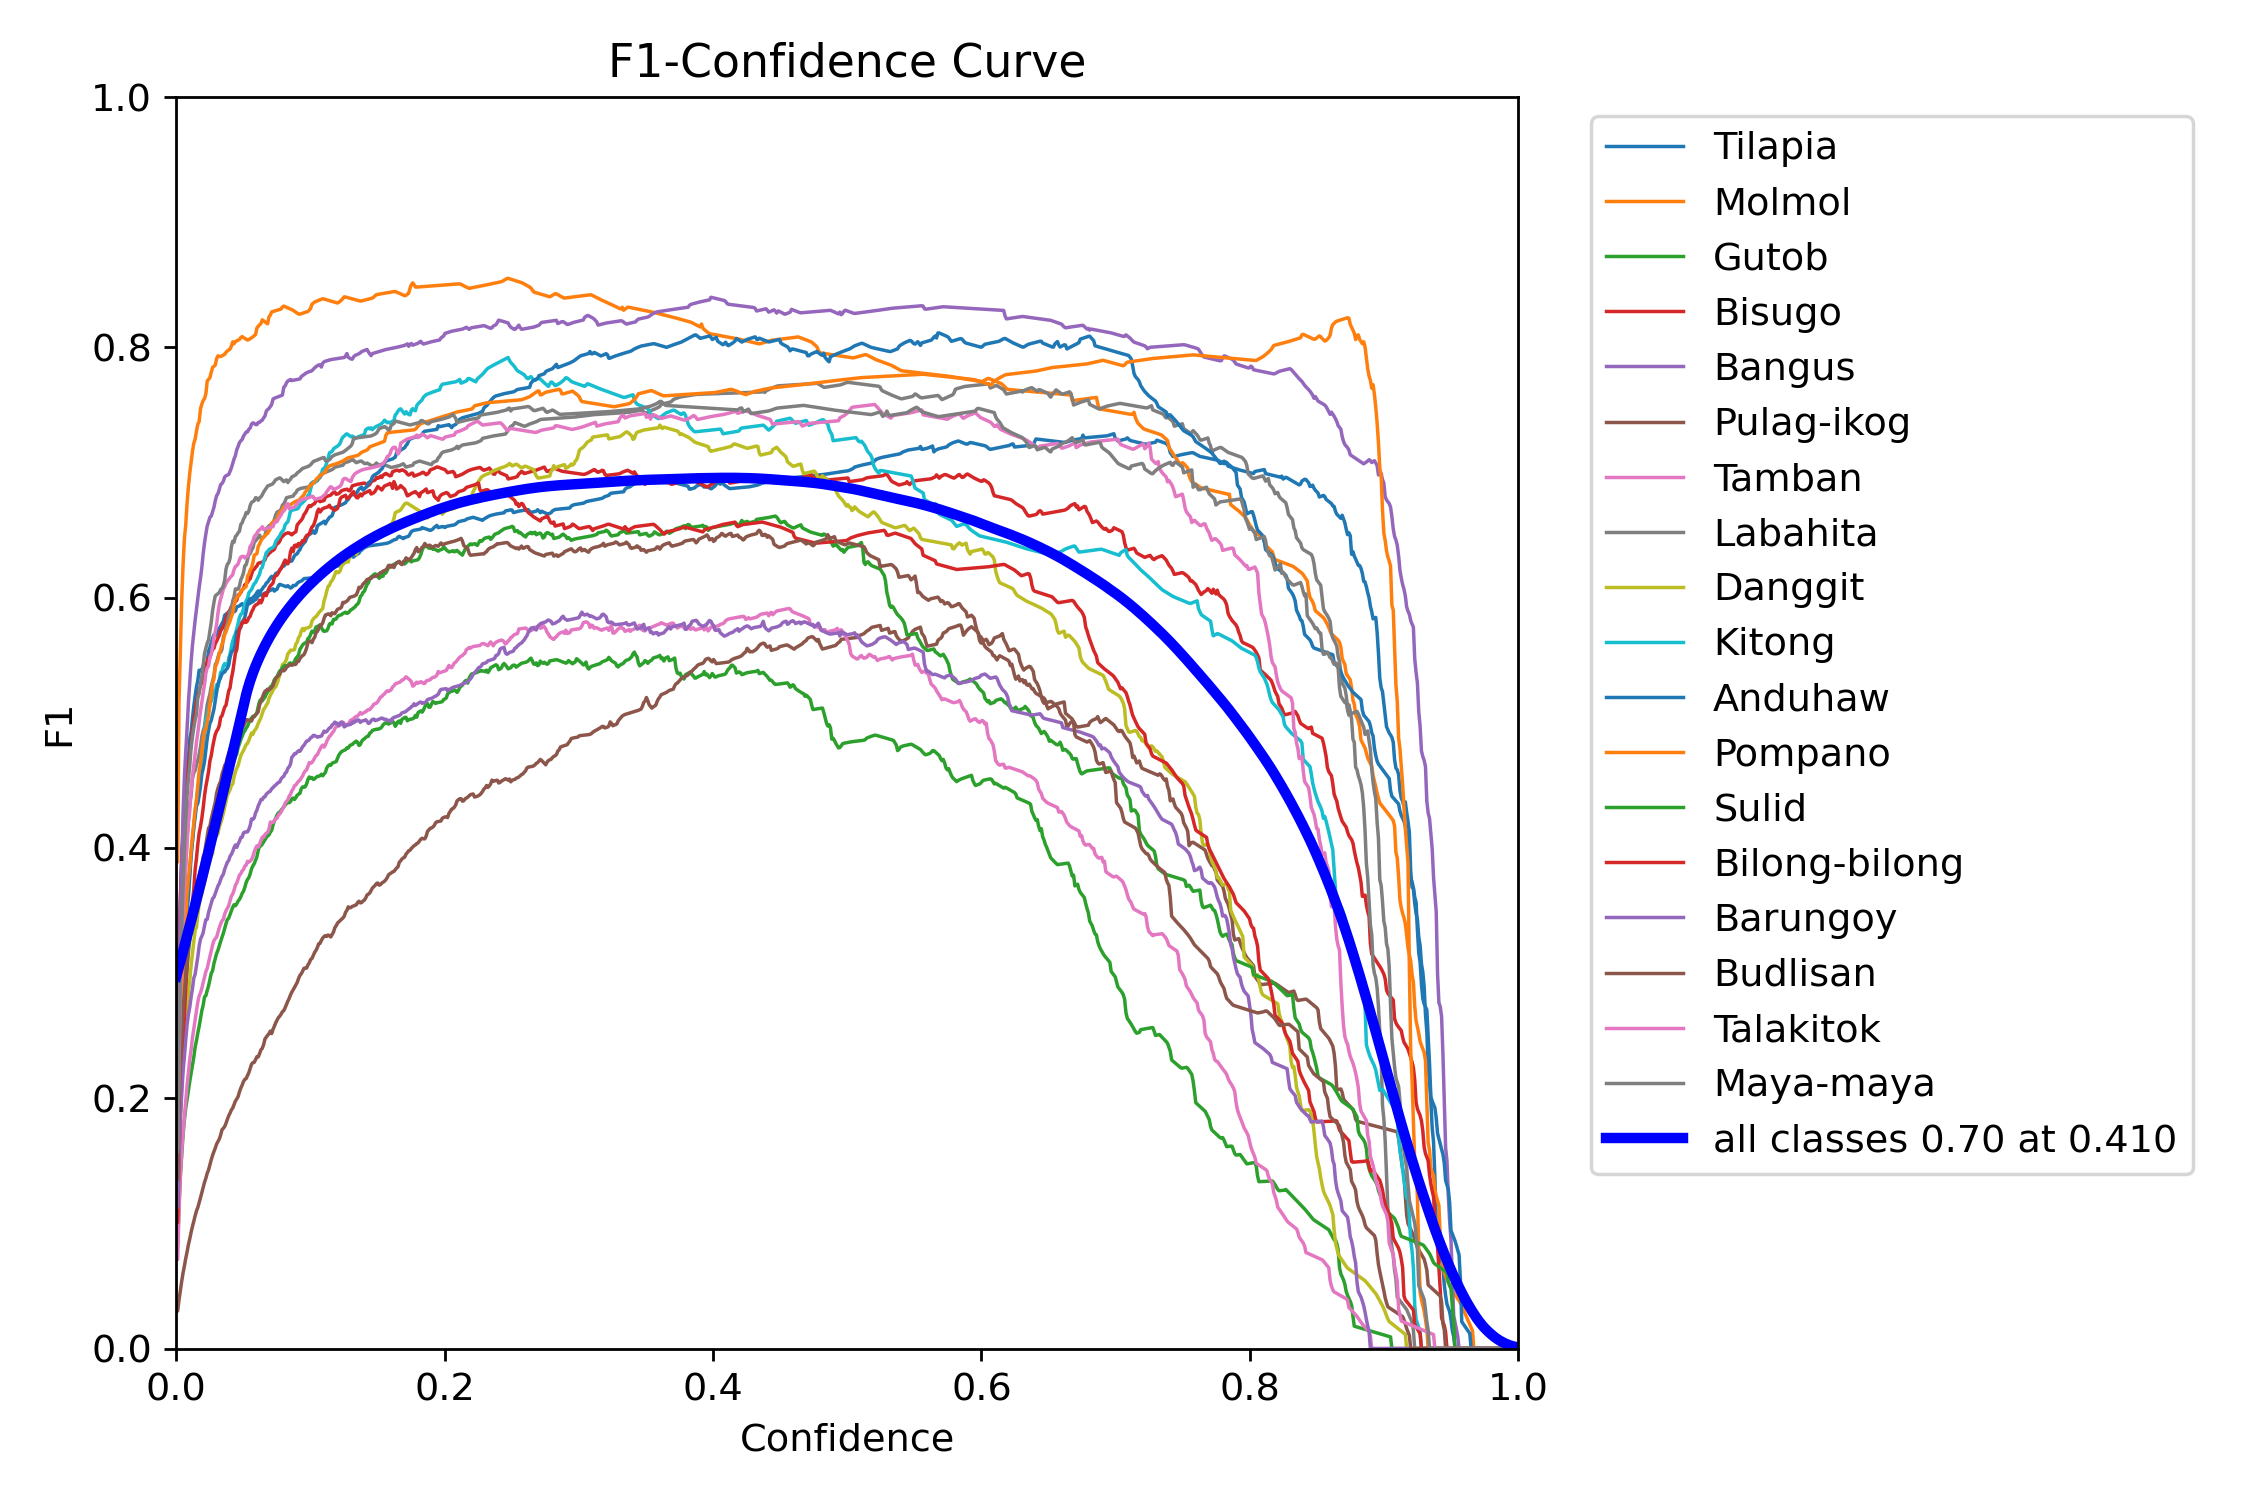
\includegraphics[width=\linewidth]{images/images/Trained/results_visualization/F1_curve.png}
        \caption*{(a) F1 Curve}
    \end{minipage}
    \hfill
    \begin{minipage}{0.8\textwidth}
        \centering
        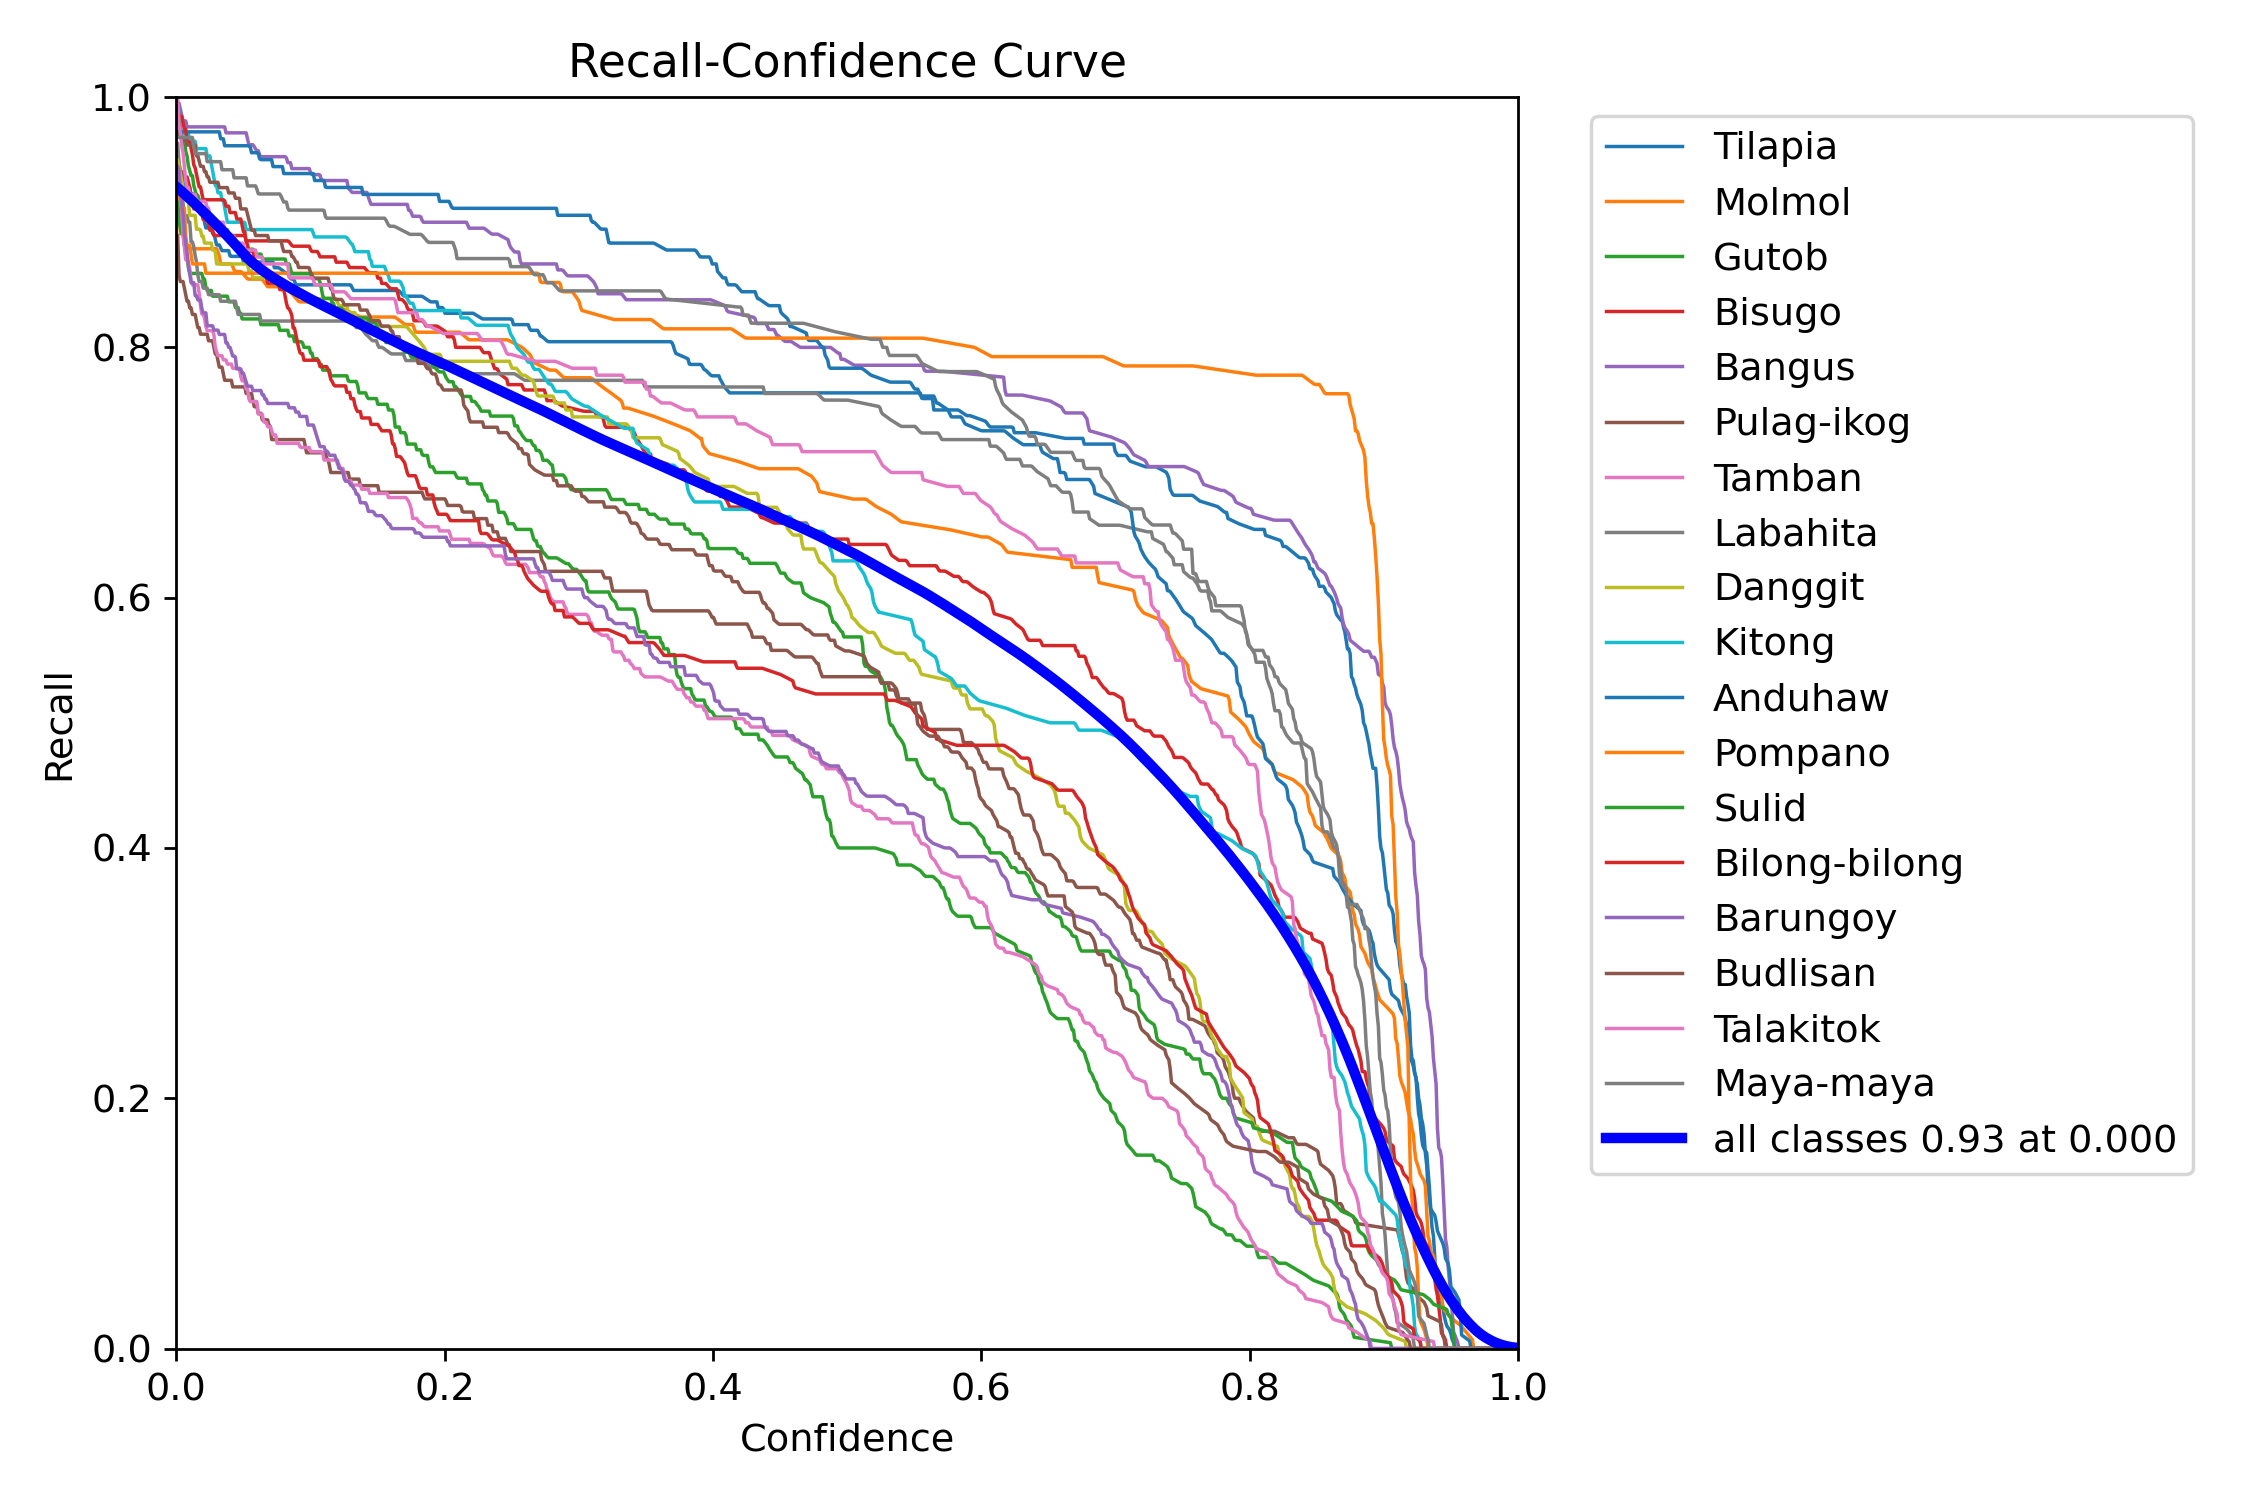
\includegraphics[width=\linewidth]{images/images/Trained/results_visualization/R_curve.png}
        \caption*{(b) Recall Curve}
    \end{minipage}
    \caption{F1 and Recall Curves Across Confidence Thresholds}
    \label{tab:F1_and_R_curve}
\end{figure}

Figure~\ref{tab:F1_and_R_curve} explains the F1 and recall curves across confidence thresholds. The F1 curve displays how the F1 score varies with different confidence thresholds, helping identify the optimal trade-off between precision and recall. The peak of this curve typically indicates the ideal threshold for model deployment. The recall curve, on the other hand, shows the decline in recall values as the confidence threshold increases. A gradual drop indicates stable model performance, while a sharp decline implies sensitivity to confidence tuning. Together, these curves assist in calibrating the model's confidence threshold for balanced and reliable predictions.

\begin{figure}[H]
    \makebox[\textwidth][c]{%
        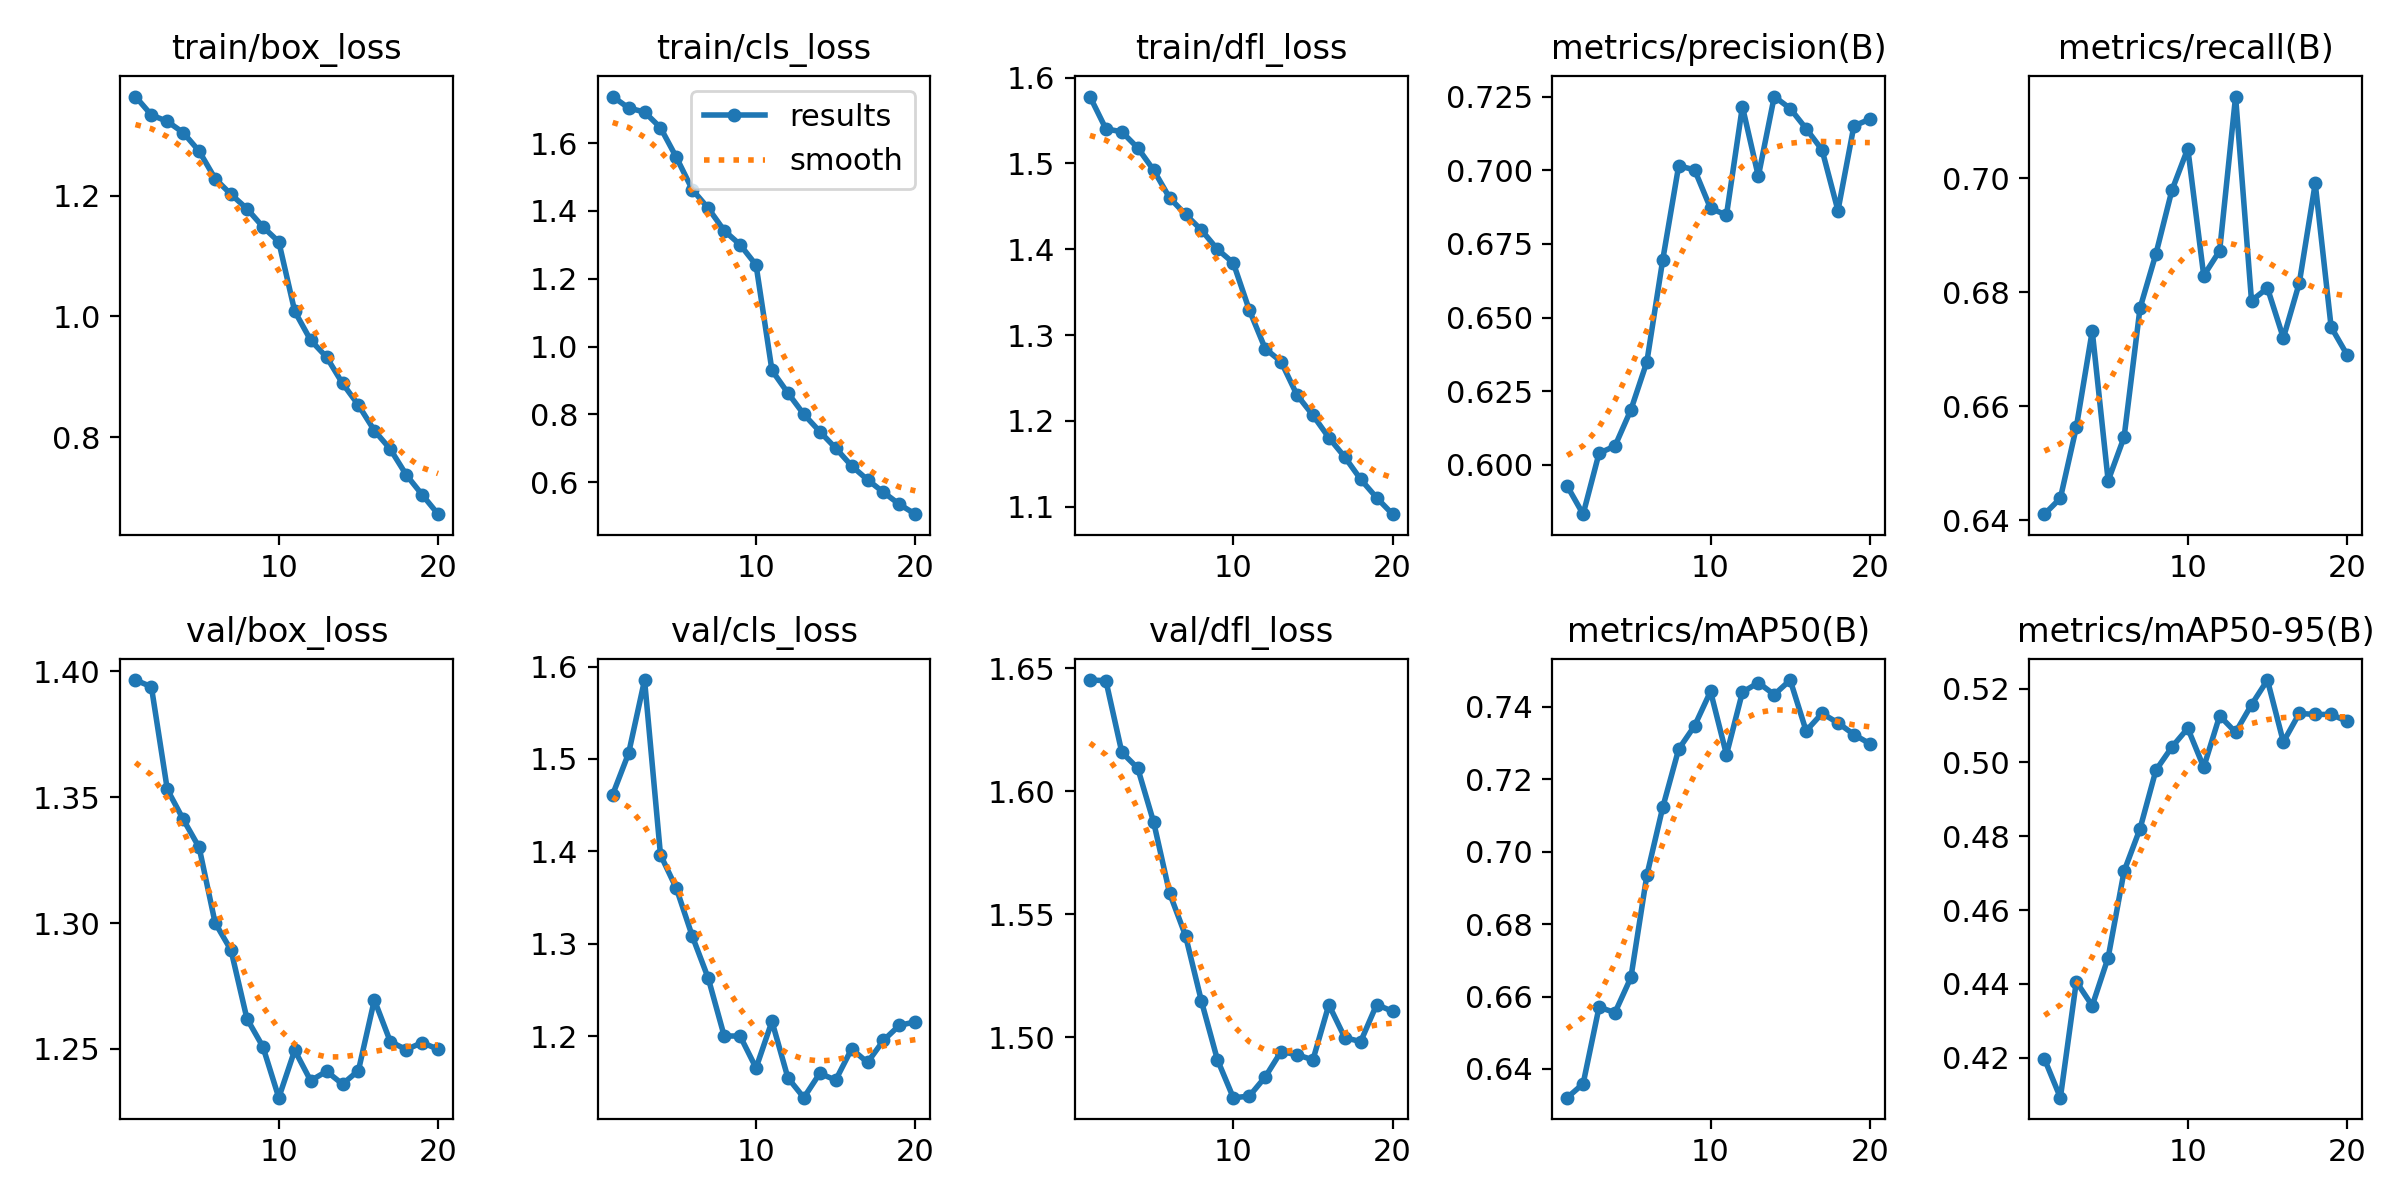
\includegraphics[width=1.1\textwidth]{images/images/Trained/results_visualization/results.png}%
    }
    \caption{Qualitative Results.}
    \label{tab:qualitative_results}
\end{figure}

Figure~\ref{tab:qualitative_results} presents the training and validation loss curves, along with evaluation metrics recorded over 30 epochs. The graphs include \texttt{train/box\_loss}, \texttt{train/cls\_loss}, and \texttt{train/dfl\_loss}, which consistently decreased, indicating effective learning and convergence of the model. Validation losses (\texttt{val/box\_loss}, \texttt{val/cls\_loss}, and \texttt{val/dfl\_loss}) also show a downward trend, suggesting that the model generalized well without significant overfitting. Additionally, the metric curves such as \texttt{metrics/precision(B)} and \texttt{metrics/recall(B)} demonstrated gradual improvements, stabilizing toward the final epochs. The evaluation metrics \texttt{metrics/mAP50(B)} and \texttt{metrics/mAP50-95(B)} also increased steadily, with the former reaching a higher value, reflecting strong localization accuracy at lower Intersection-over-Union (IoU) thresholds. These trends collectively confirm the model's robustness and effectiveness in both training and validation phases.


\subsection{Visual Comparison: Ground Truth vs. Predicted Bounding Boxes}
To provide a visual assessment of the model’s detection capability, a comparison between the ground truth and predicted bounding boxes for each of the 18 fish species is presented. These sample images were drawn from the test set and demonstrate the model’s ability to localize and classify species accurately.

Figures~\ref{fig: Bangus} to Figure~\ref{fig:Labahita}  show a side-by-side comparison of ground truth and predicted bounding boxes for the fish species. The left image shows manually annotated (ground truth) labels, and the right image shows predictions by the YOLOv11 model. Green boxes indicate predicted species with confidence scores, and blue boxes indicate ground truth annotations.

\begin{figure}[H]
    \centering
    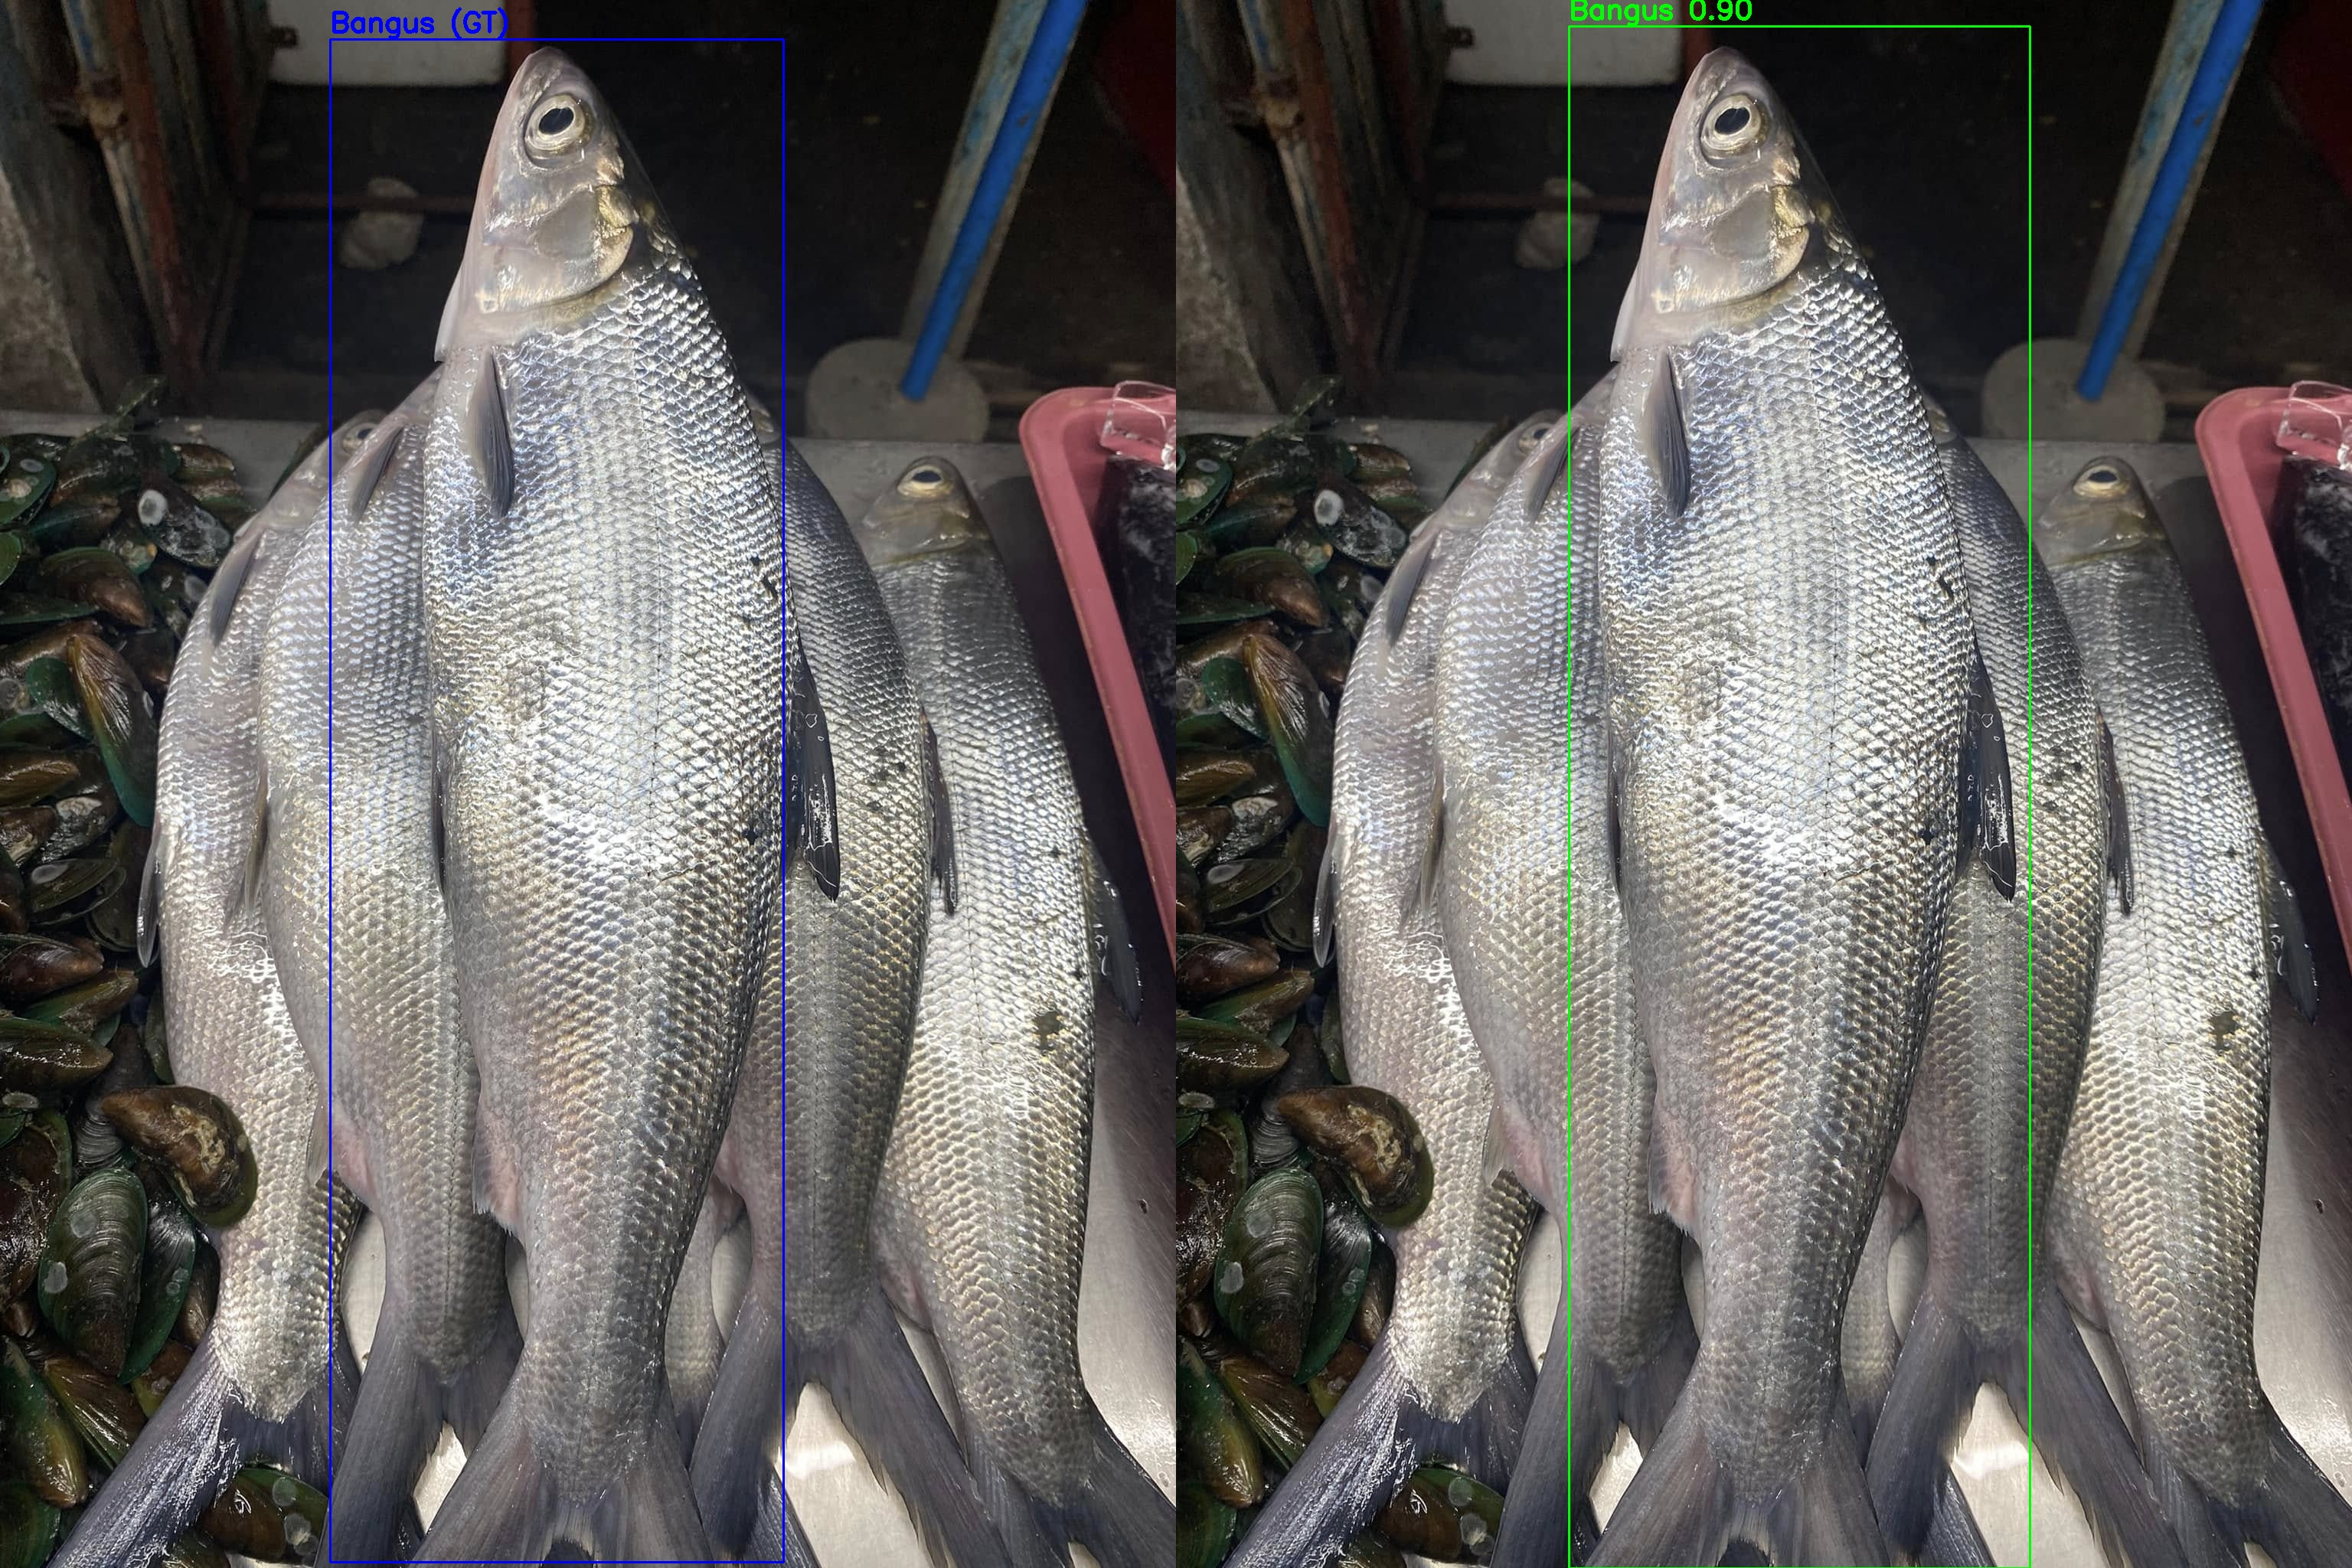
\includegraphics[width=0.8\textwidth]{images/images/predictions_per_class/Bangus_compare_7.jpg}
    \caption{Ground Truth vs. Predicted Bounding Boxes for Bangus} 
    \label{fig: Bangus}
\end{figure}

\begin{figure}[H]
    \centering
    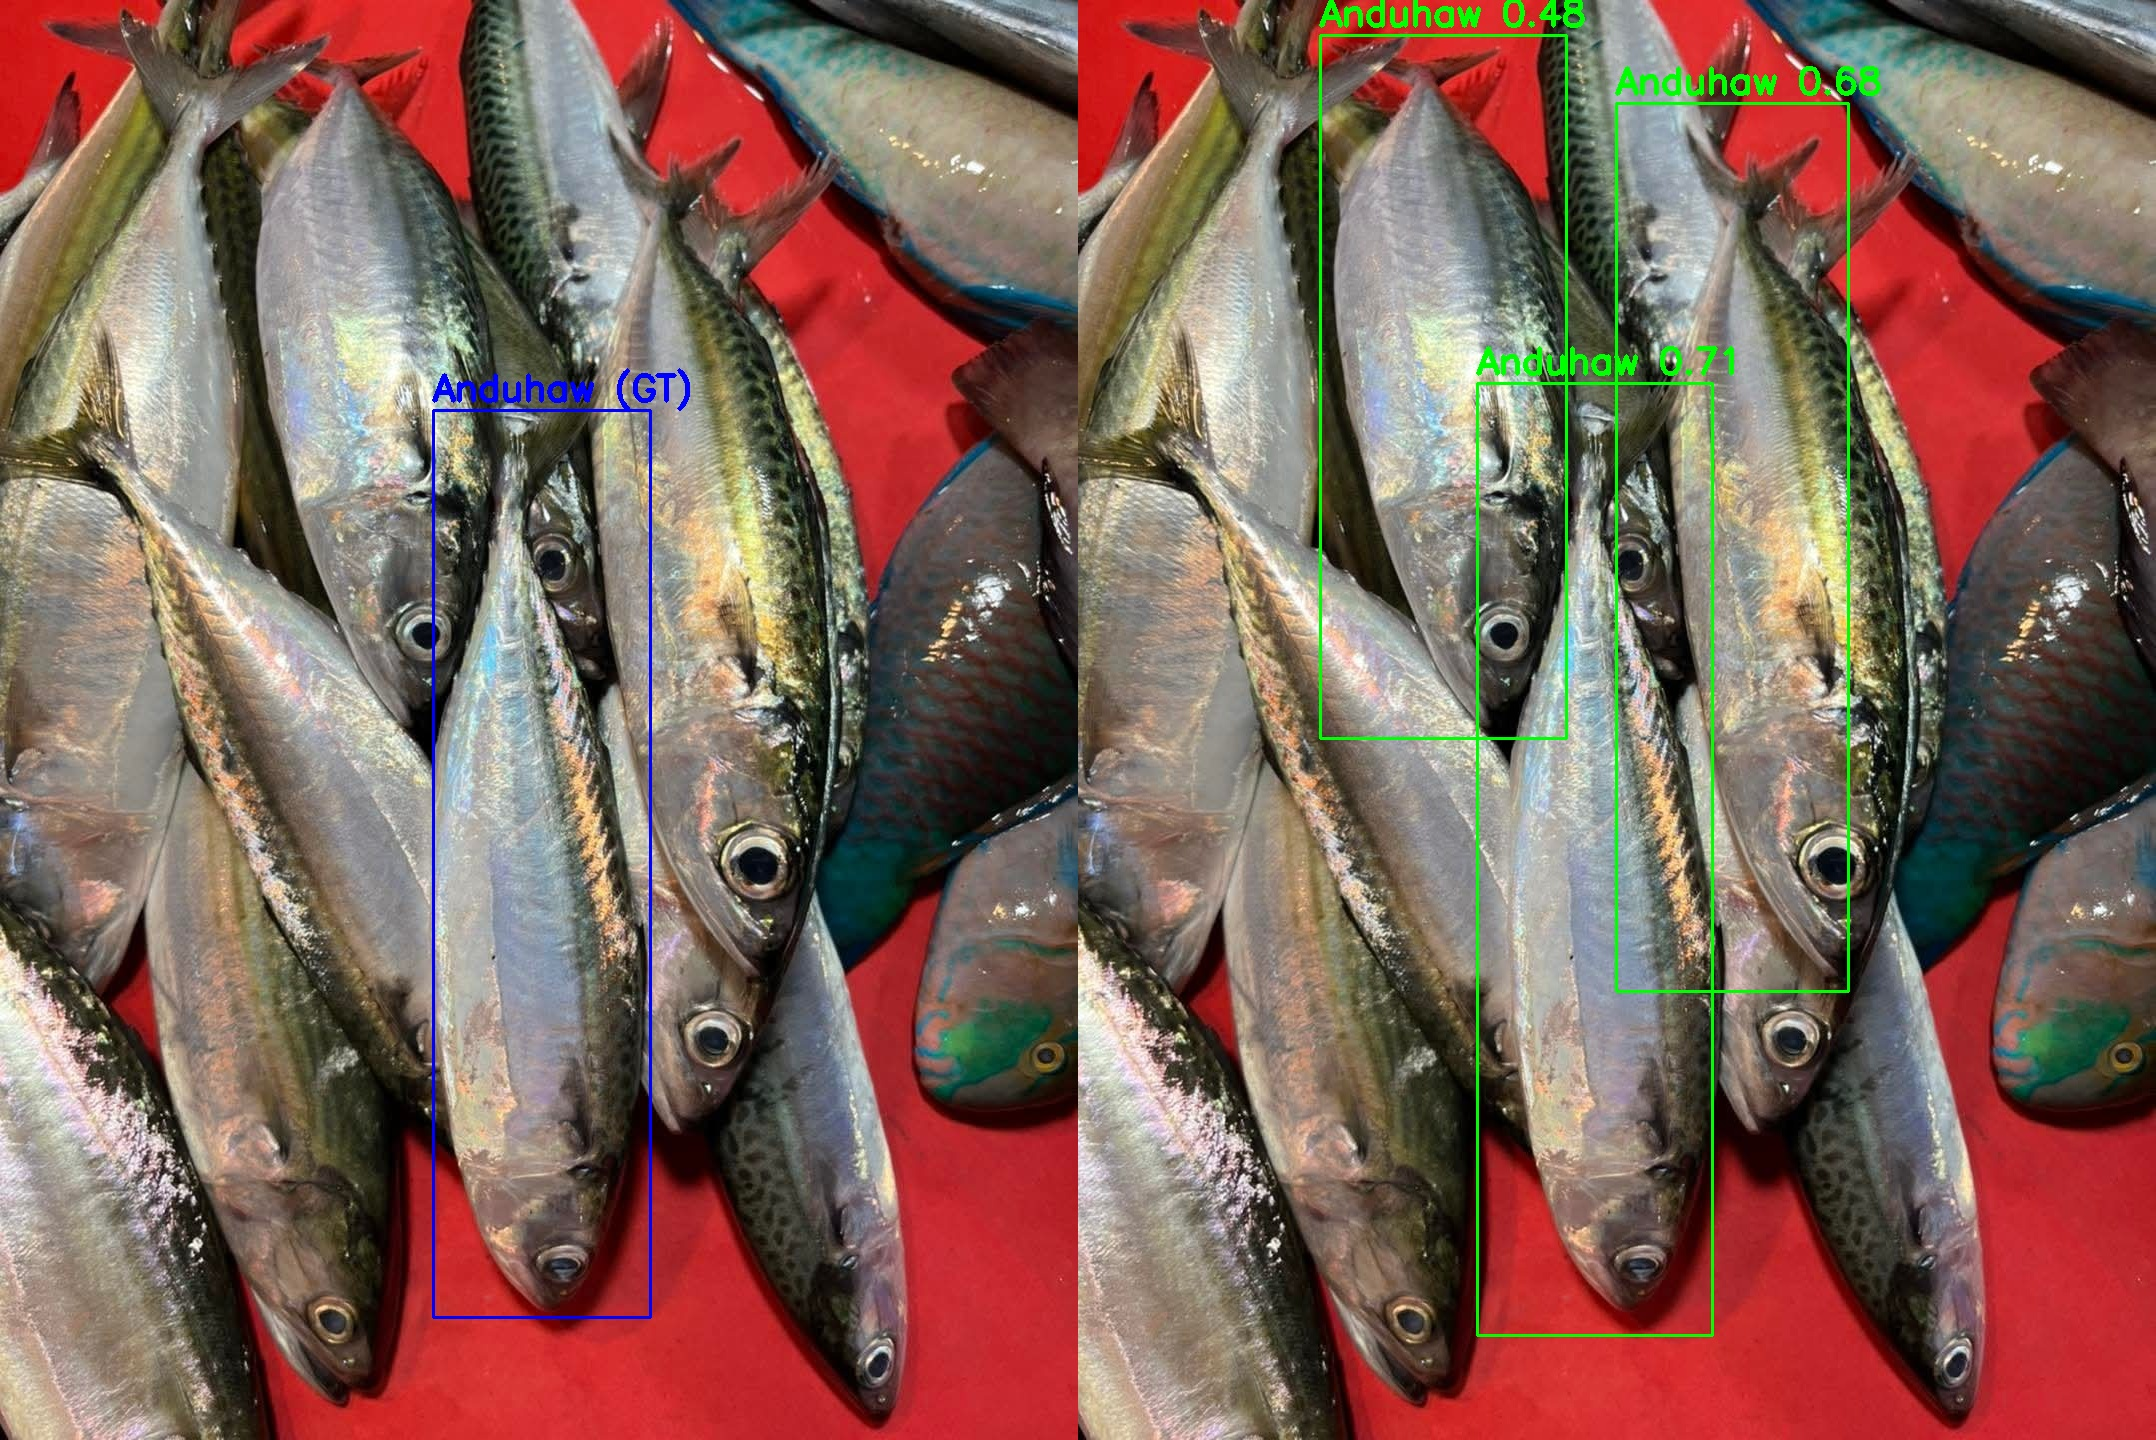
\includegraphics[width=0.8\textwidth]{images/images/predictions_per_class/Anduhaw_compare_19.jpg}
    \caption{Ground Truth vs. Predicted Bounding Boxes for Anduhaw} 
    \label{fig: Anduhaw}
\end{figure}

\begin{figure}[H]
    \centering
    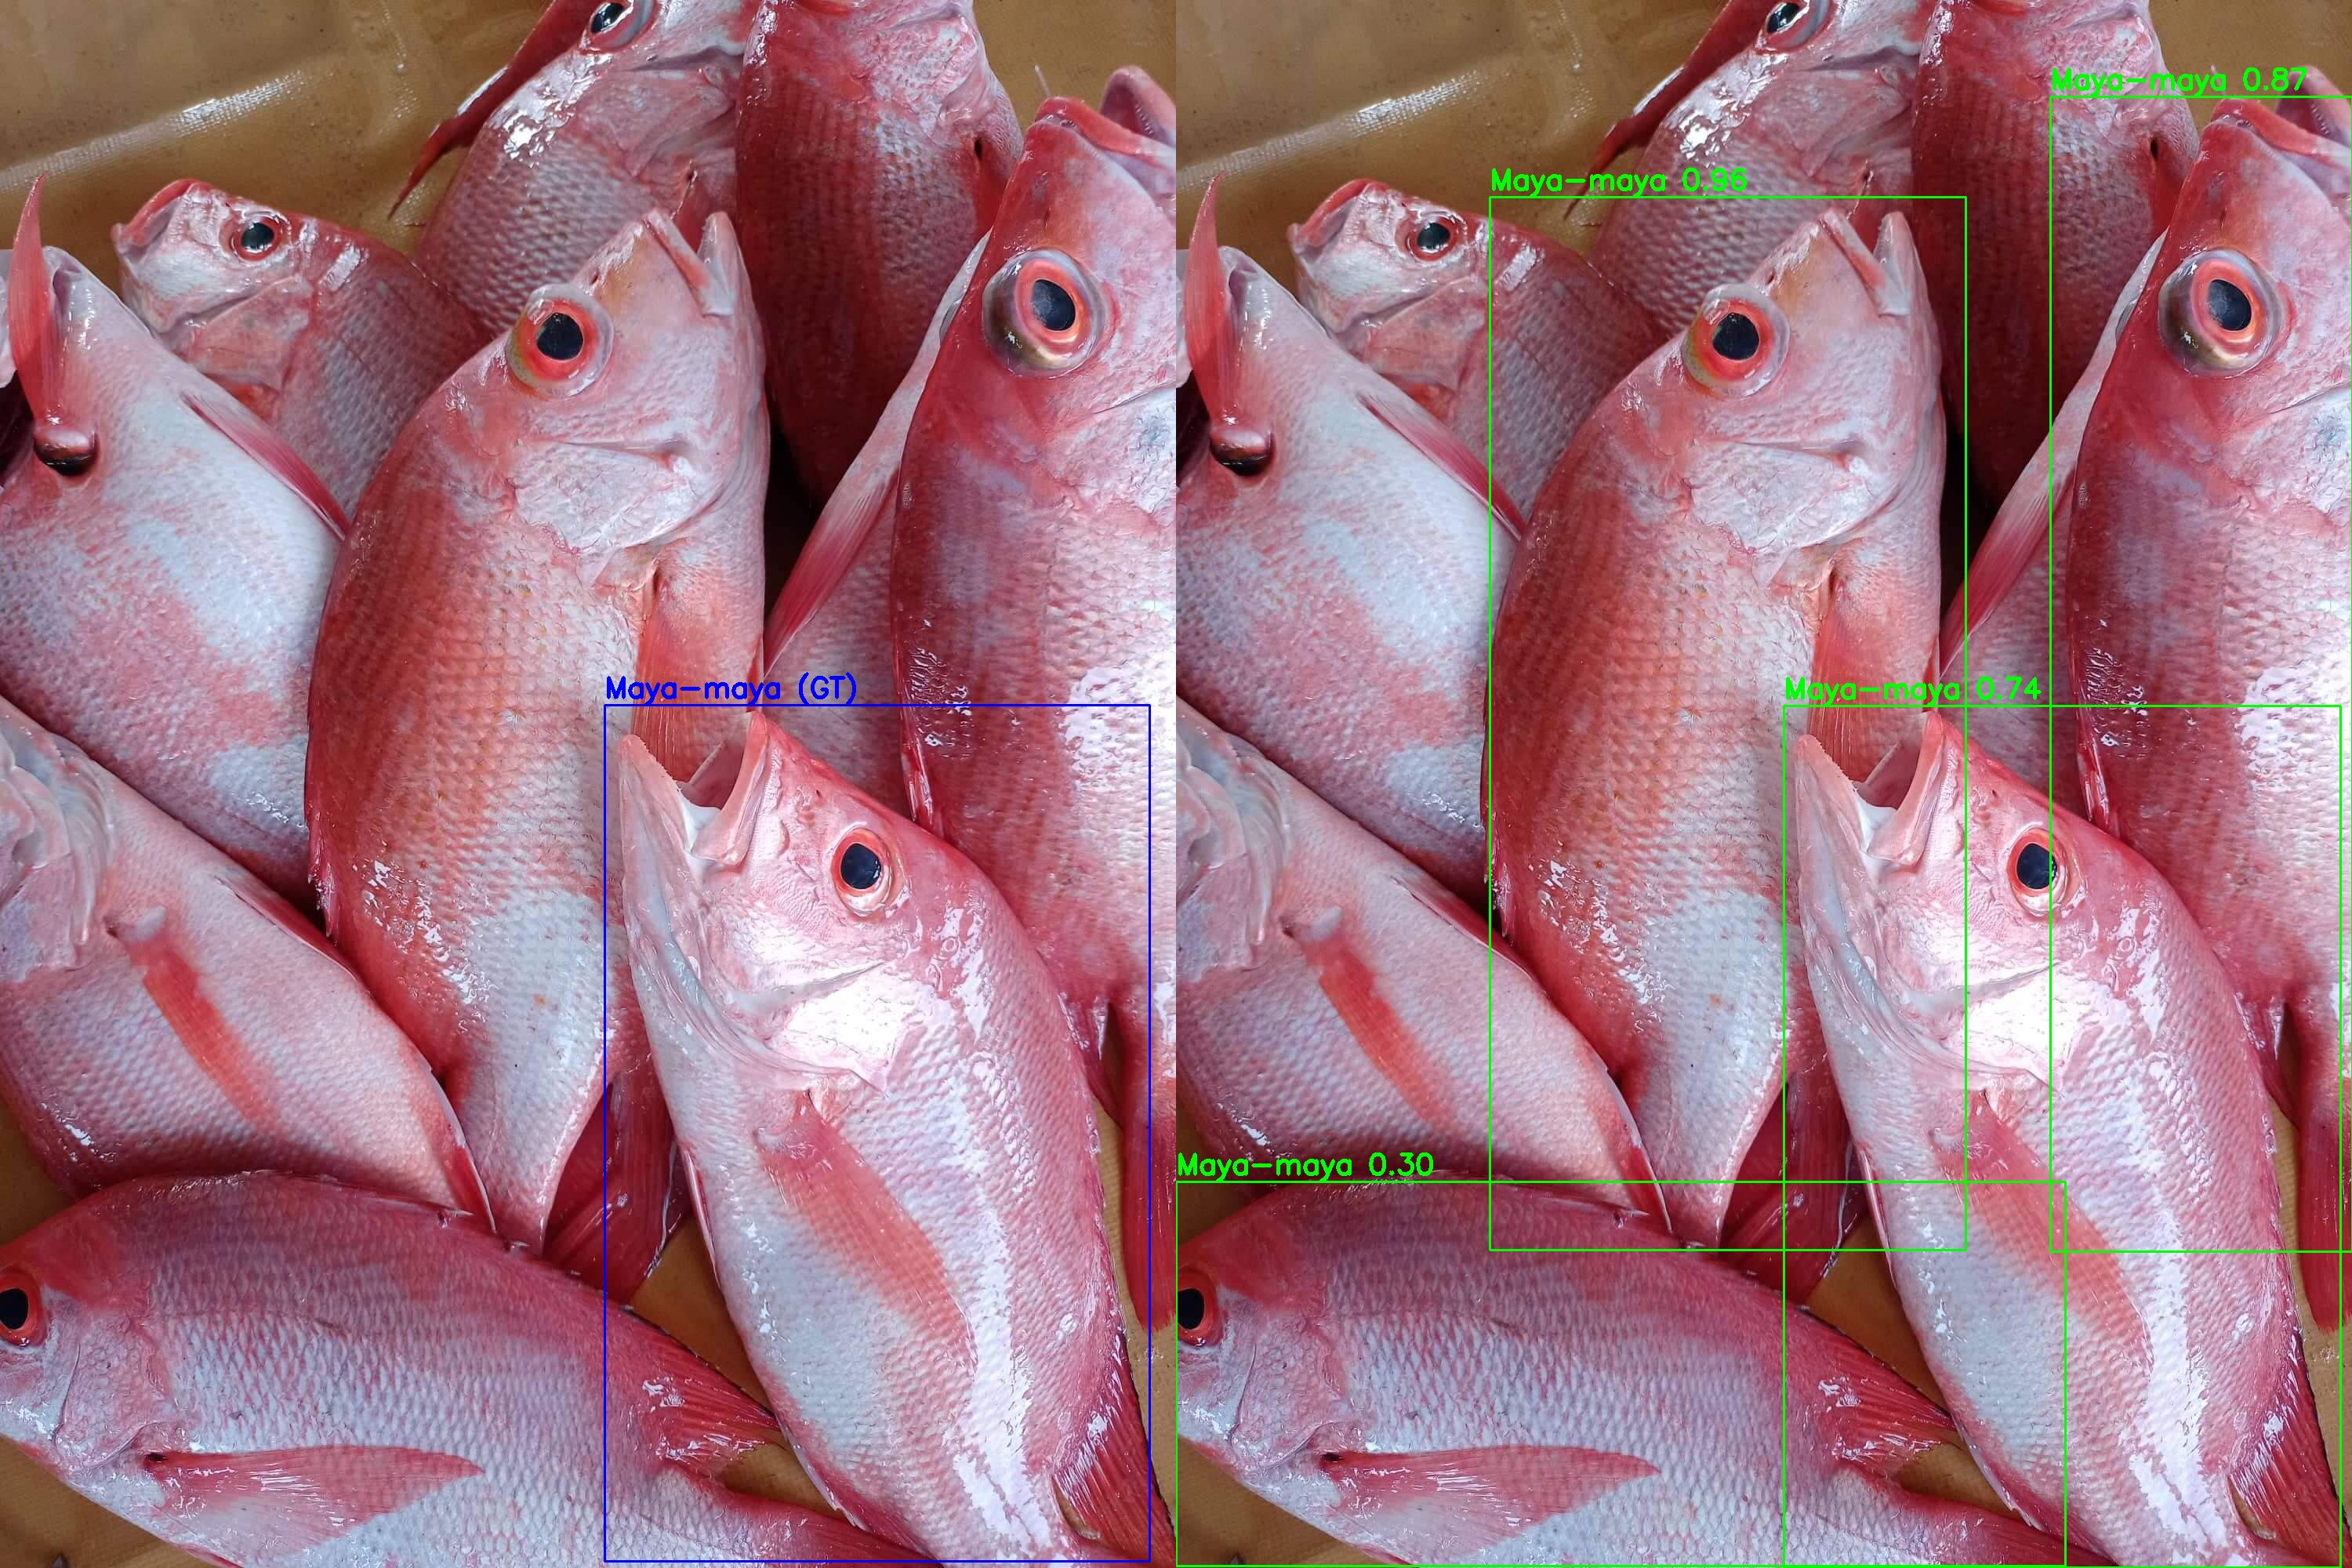
\includegraphics[width=0.8\textwidth]{images/images/predictions_per_class/Maya-maya_compare_13.jpg}
    \caption{Ground Truth vs. Predicted Bounding Boxes for Maya-maya} 
    \label{fig: Maya-maya}
\end{figure}

\begin{figure}[H]
    \centering
    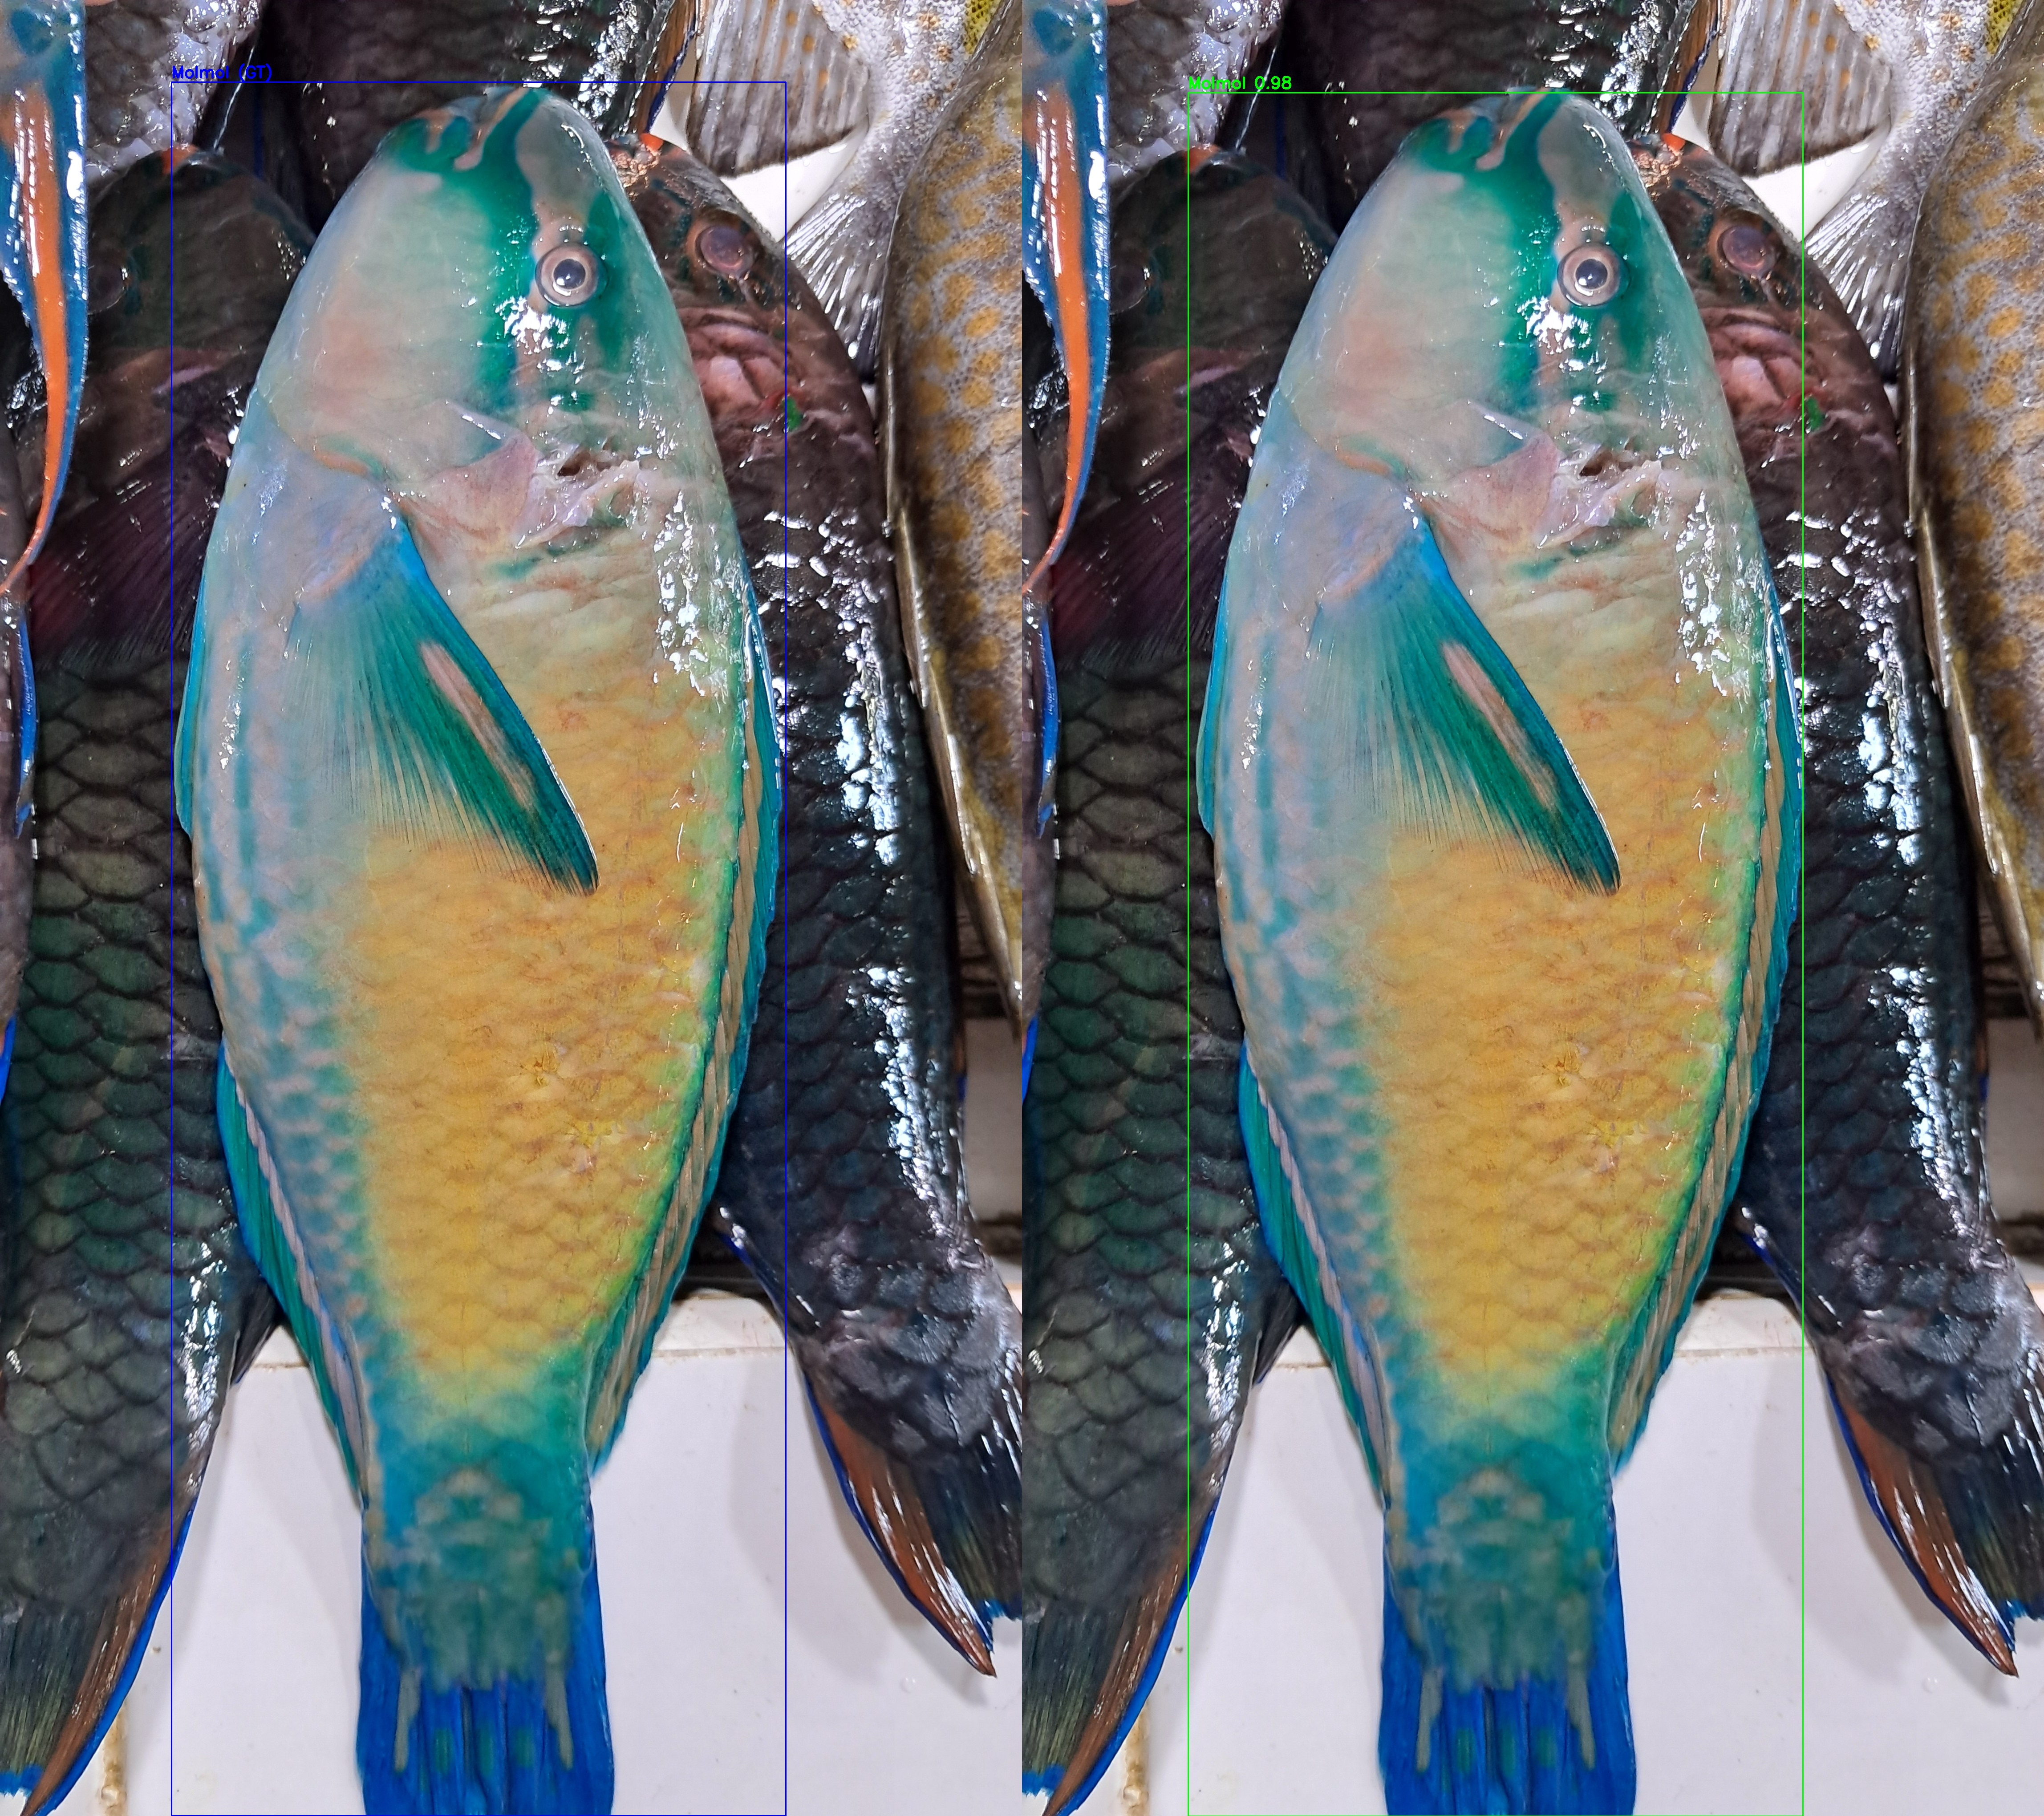
\includegraphics[width=0.8\textwidth]{images/images/predictions_per_class/Labeled_Molmol_Detected_Molmol.jpg}
    \caption{Ground Truth vs. Predicted Bounding Boxes for Molmol} 
    \label{fig: Molmol}
\end{figure}

\begin{figure}[H]
    \centering
    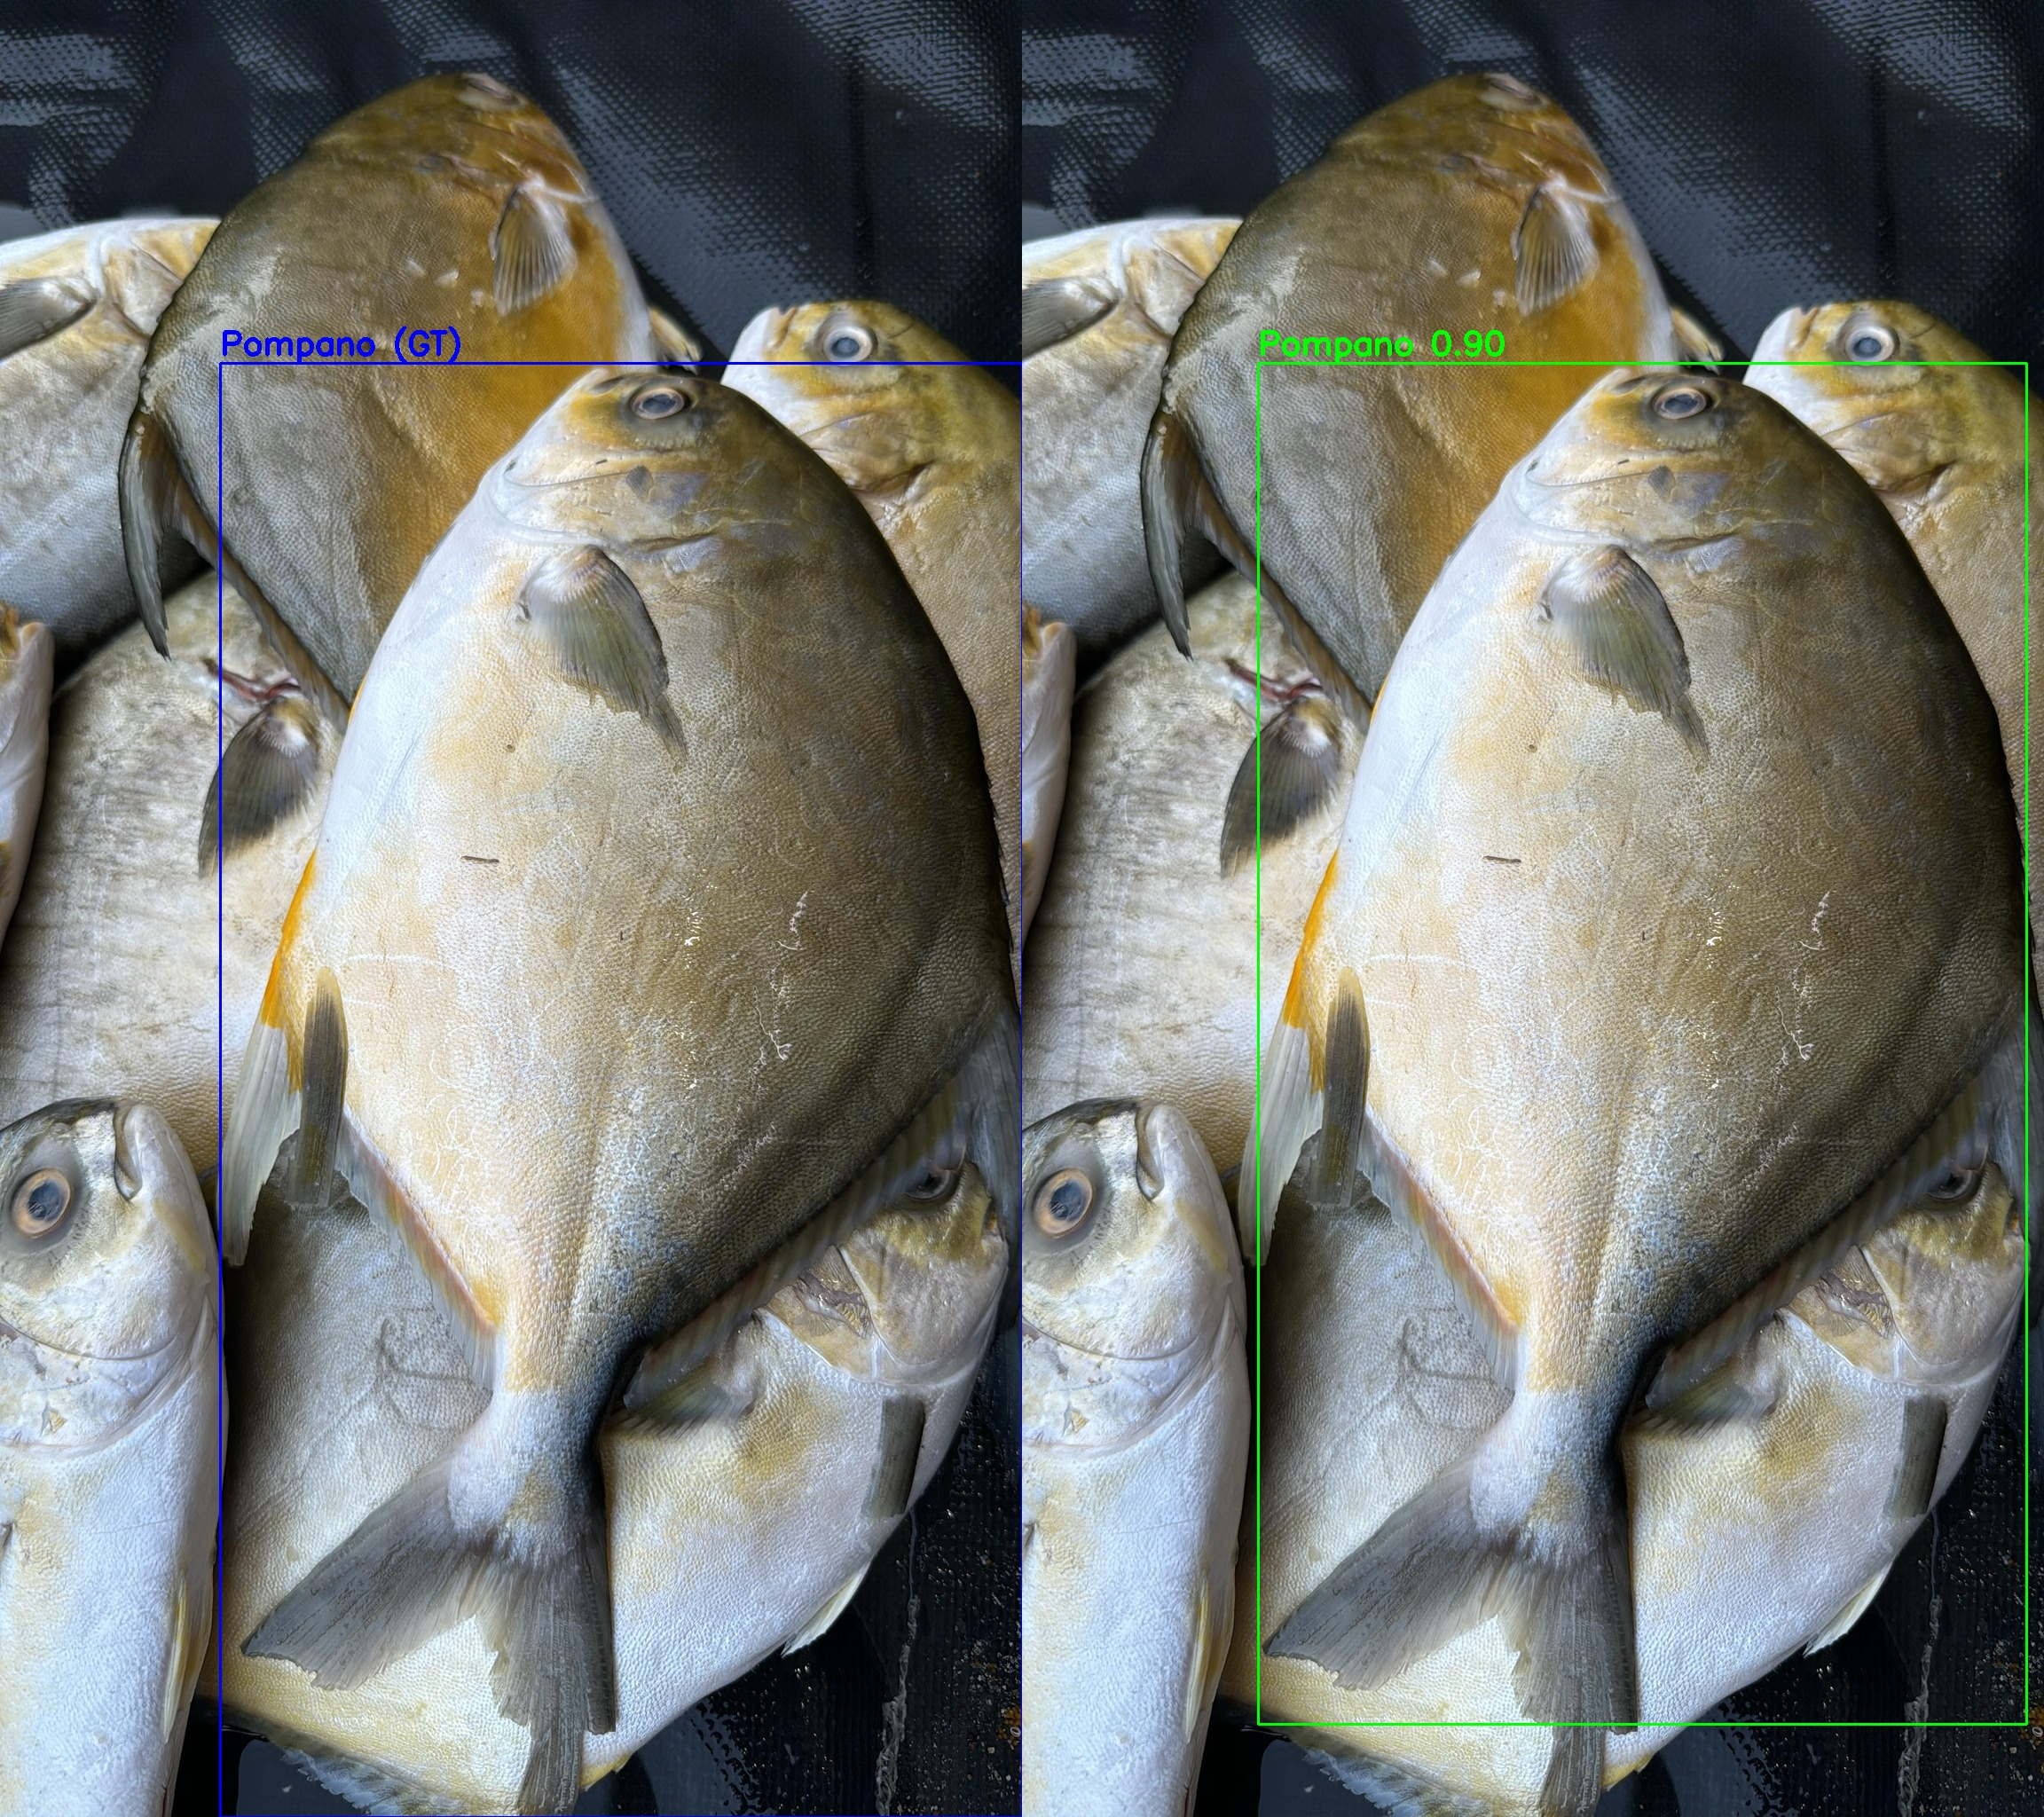
\includegraphics[width=0.8\textwidth]{images/images/predictions_per_class/Labeled_Pompano_Detected_Pompano.jpg}
    \caption{Ground Truth vs. Predicted Bounding Boxes for Pompano} 
    \label{fig: Pompano}
\end{figure}

\begin{figure}[H]
    \centering
    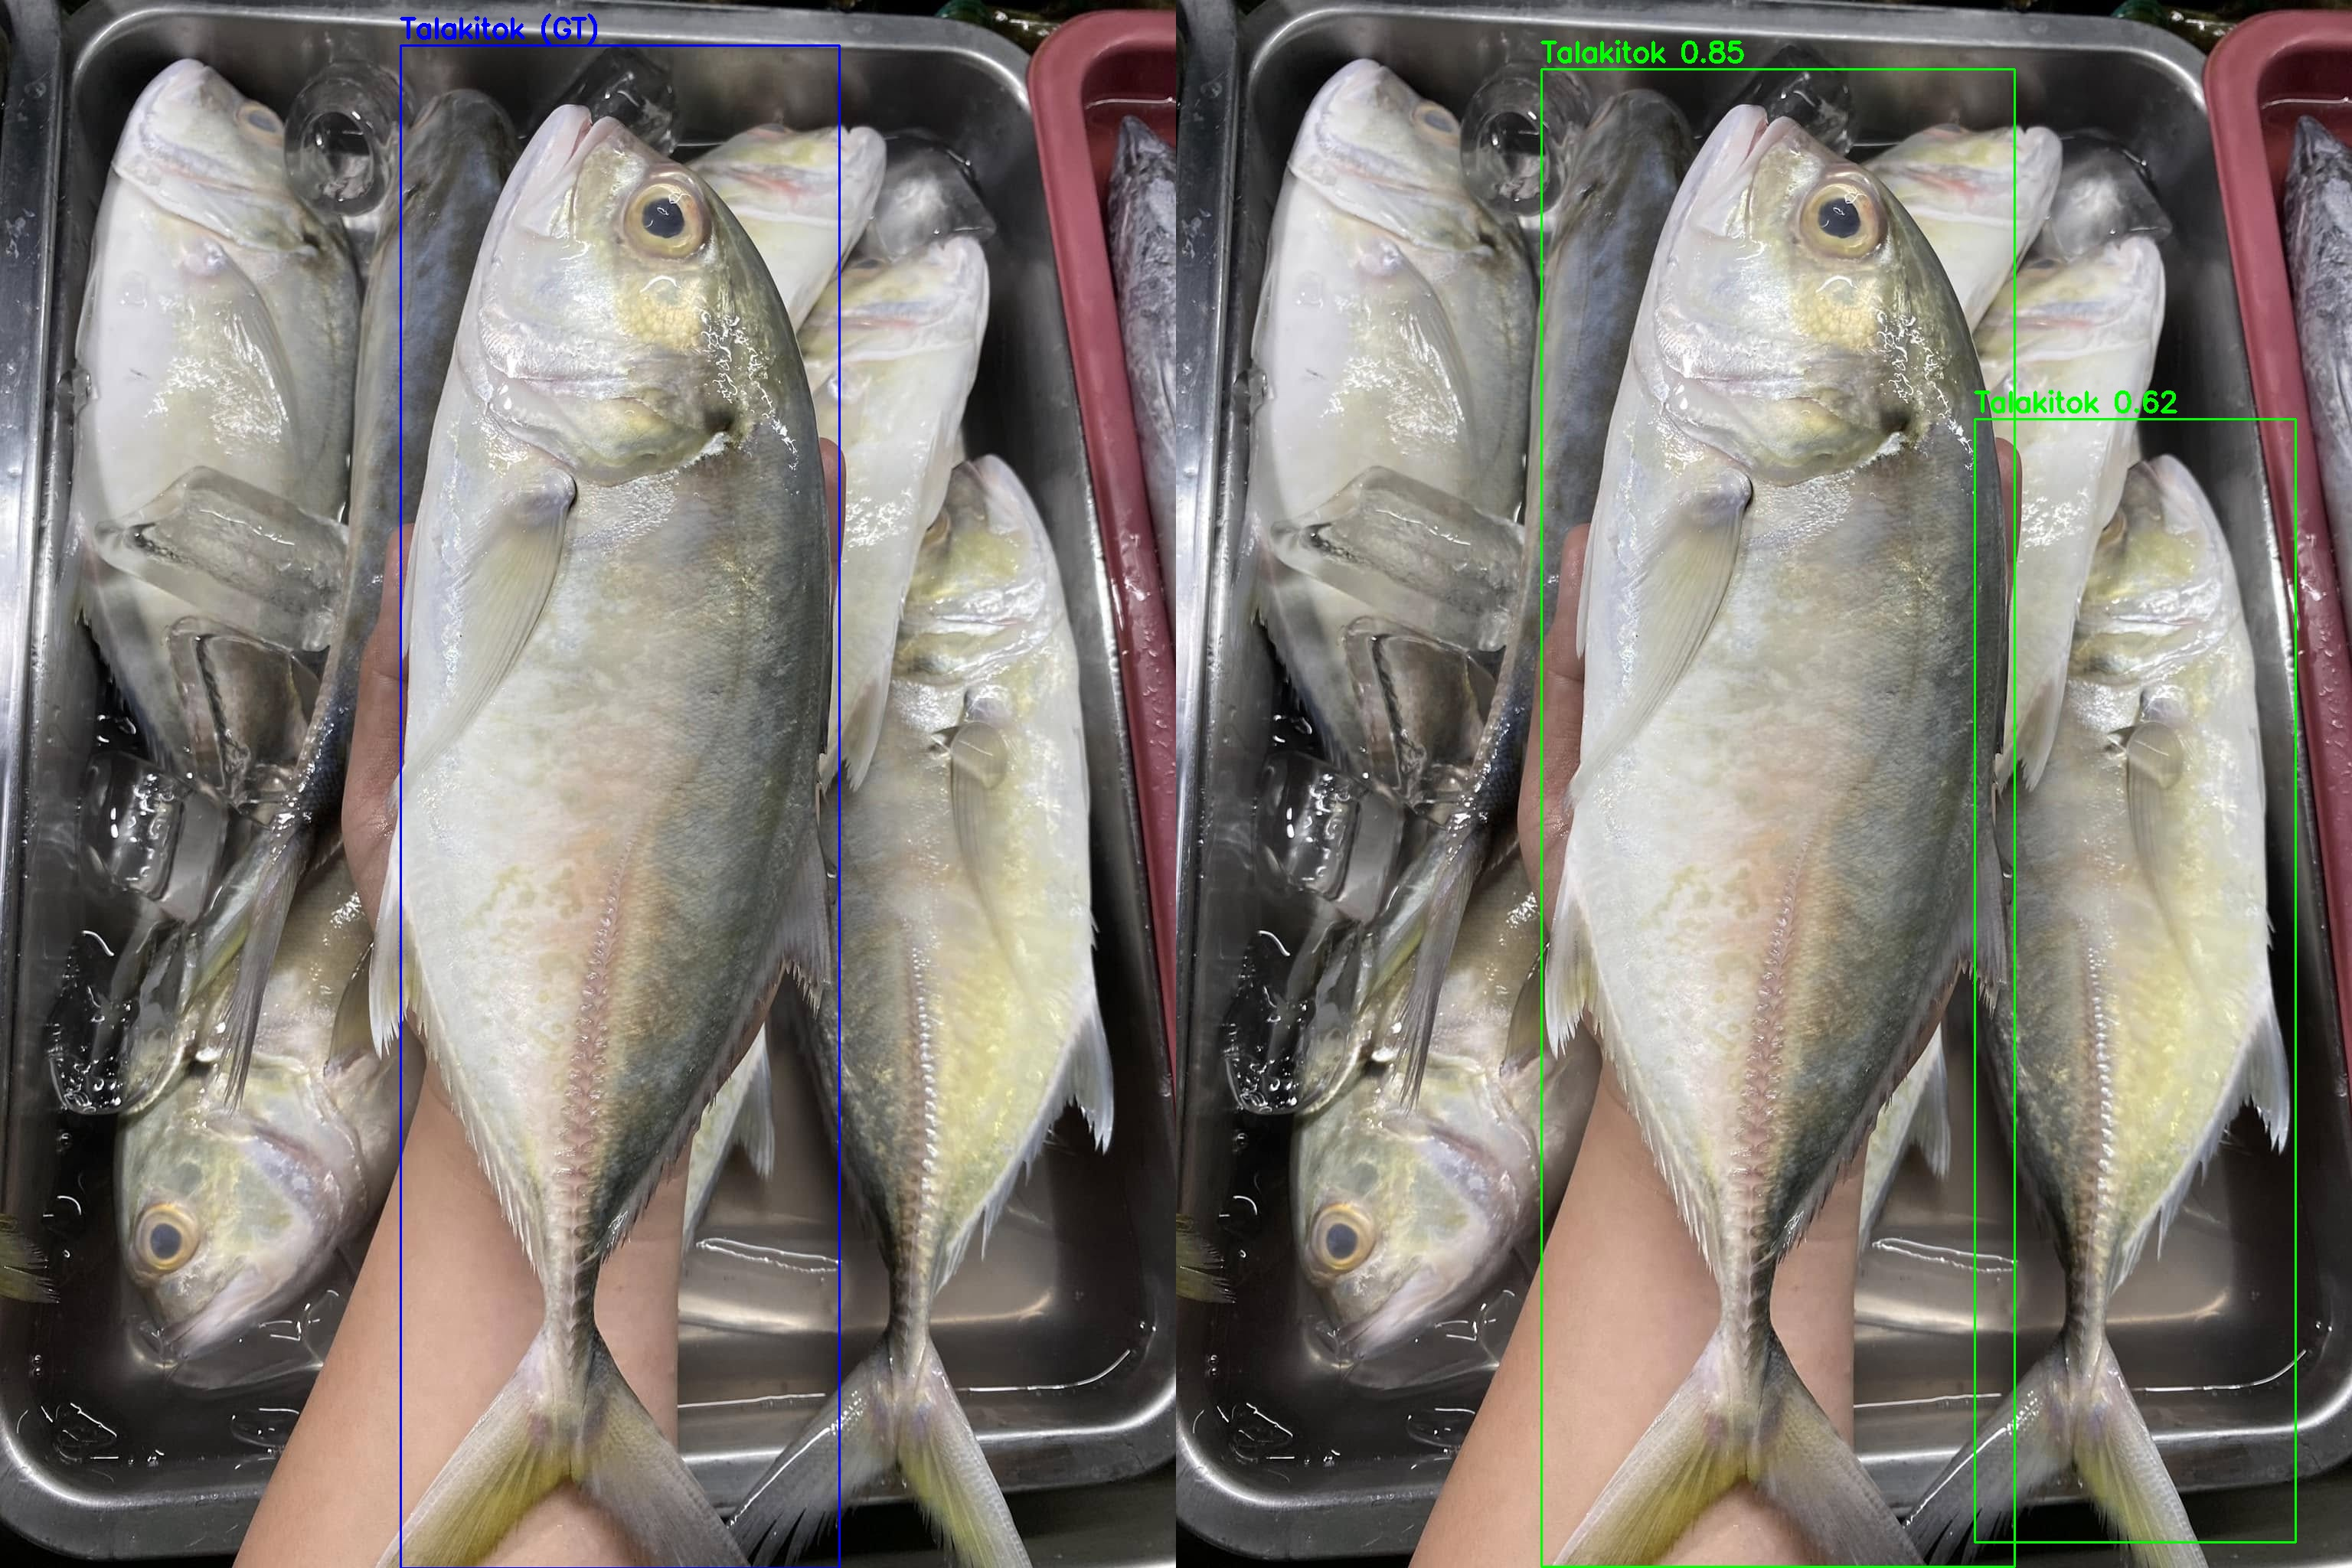
\includegraphics[width=0.8\textwidth]{images/images/predictions_per_class/Talakitok_compare_6.jpg}
    \caption{Ground Truth vs. Predicted Bounding Boxes for Talakitok} 
    \label{fig:Talakitok}
\end{figure}
\begin{figure}[H]
    \centering
    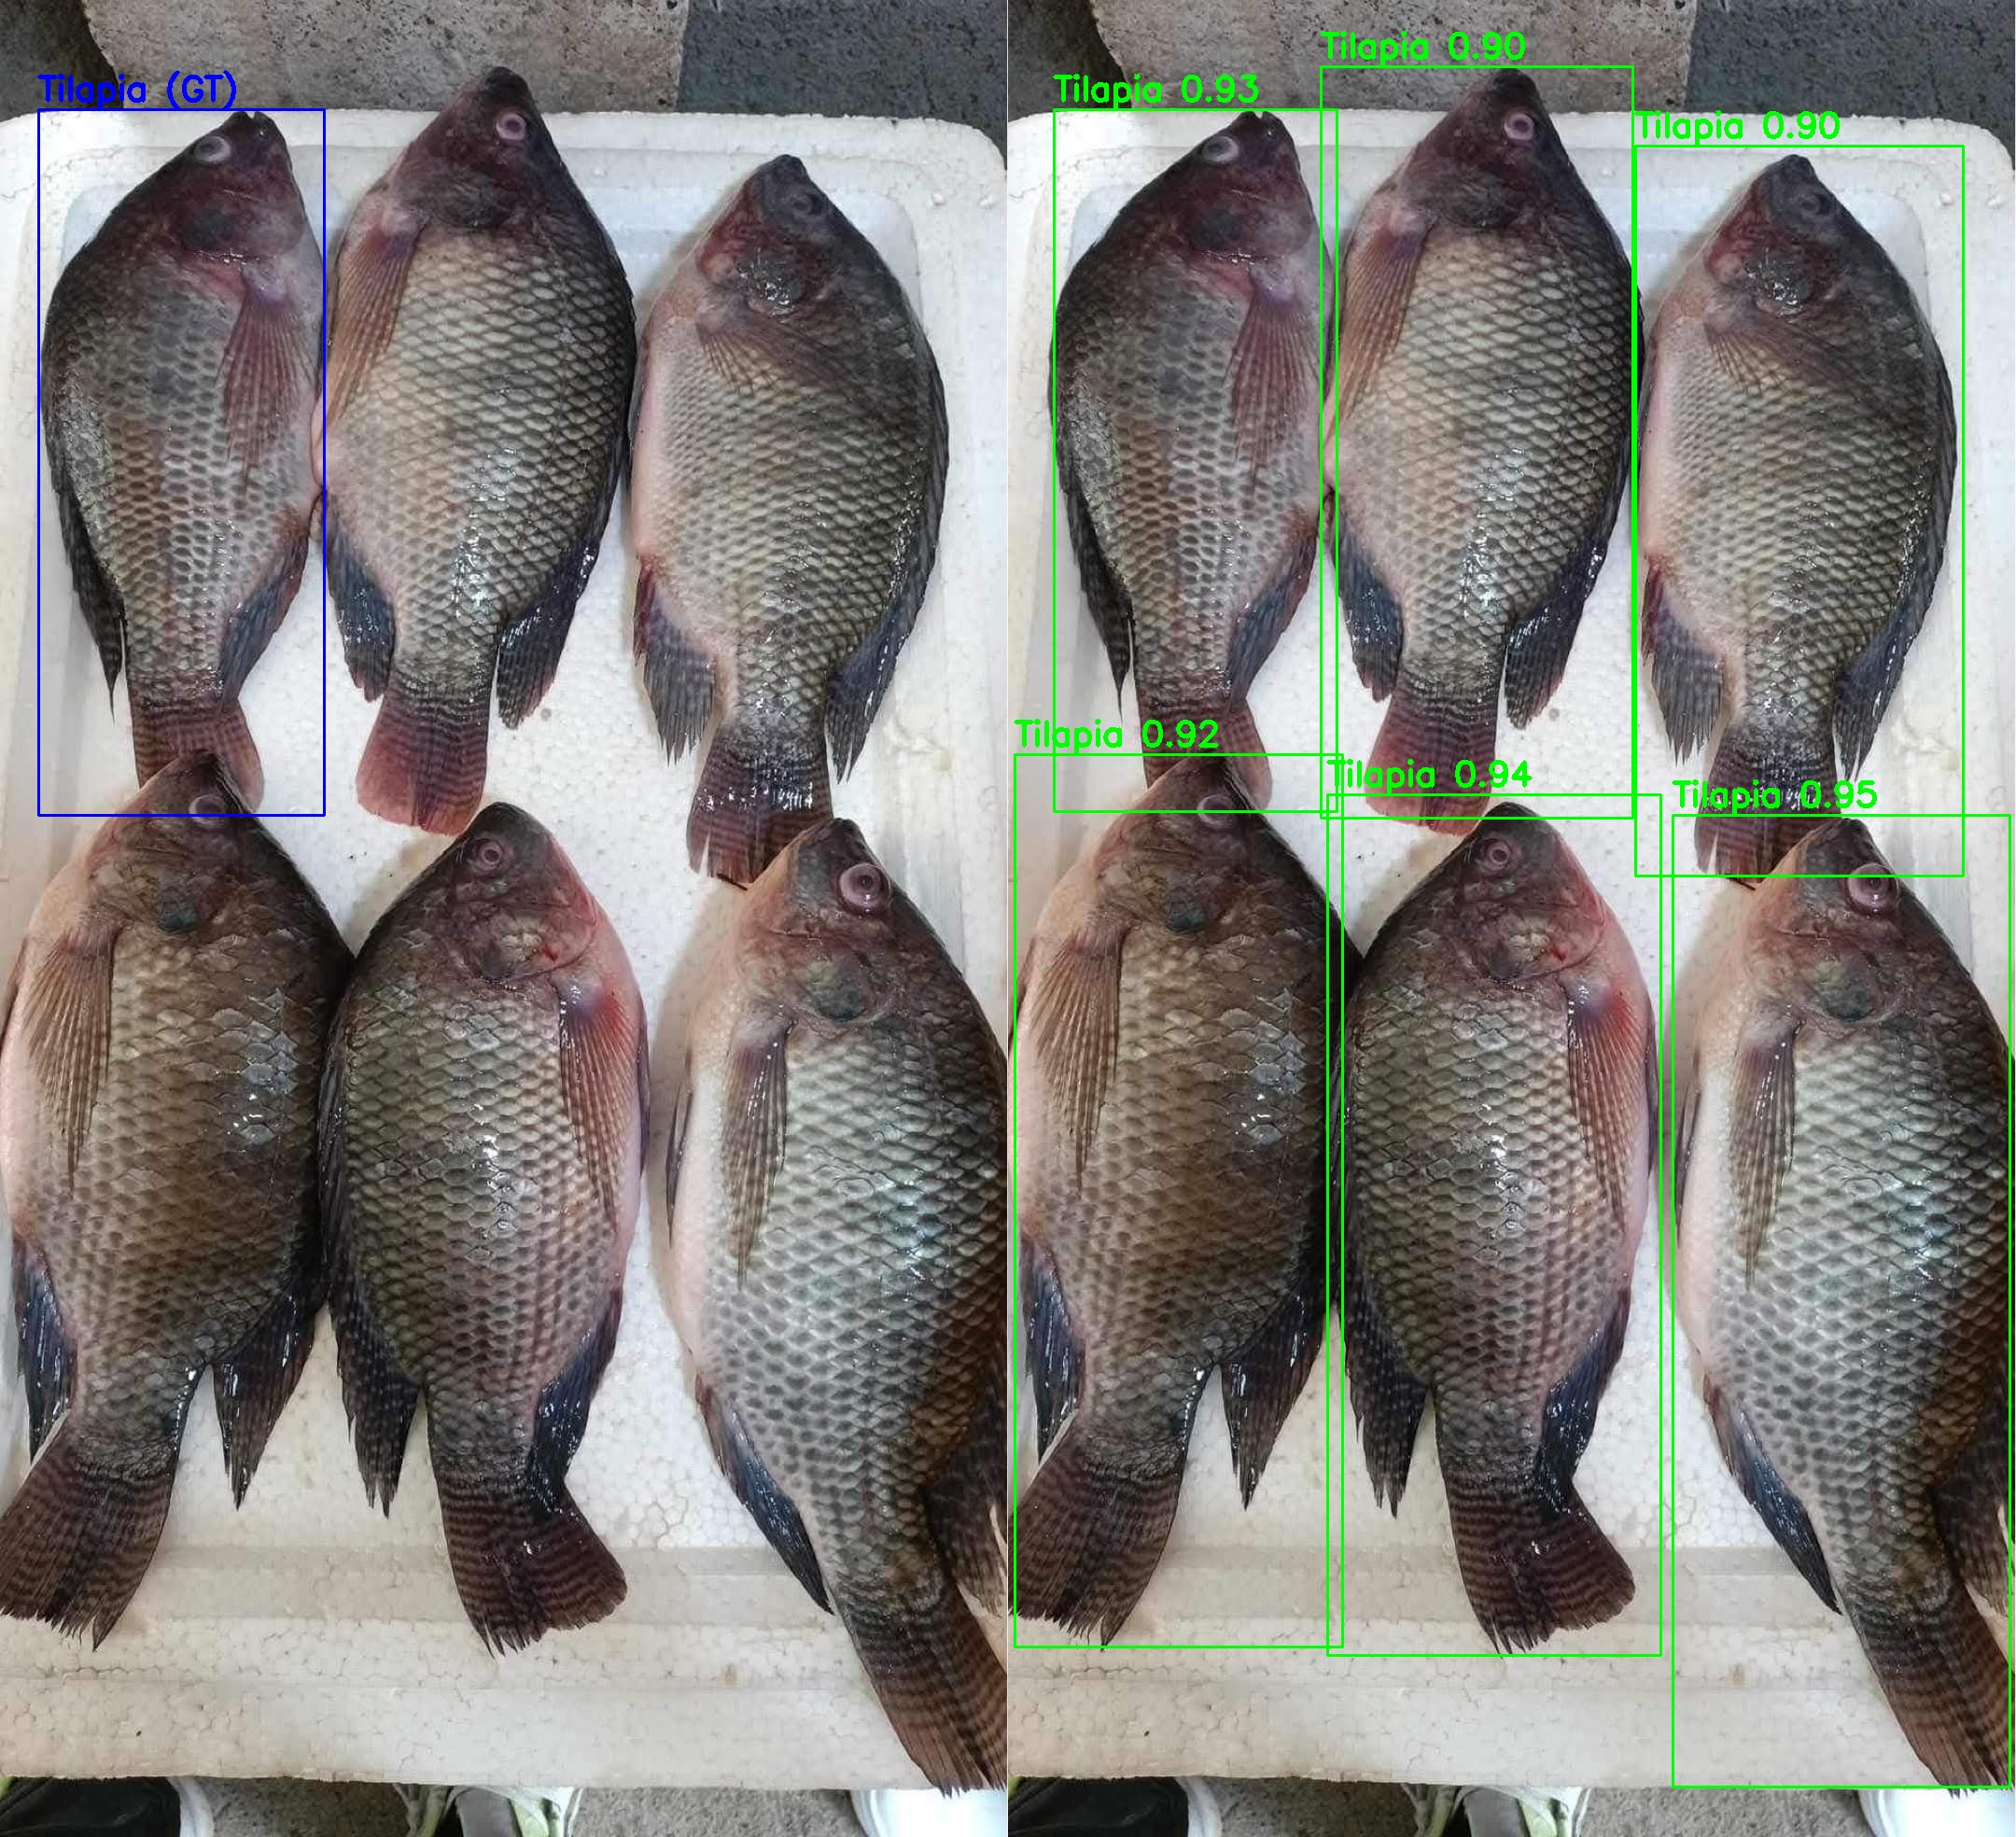
\includegraphics[width=0.8\textwidth]{images/images/predictions_per_class/Labeled_Tilapia_Detected_Tilapia.jpg}
    \caption{Ground Truth vs. Predicted Bounding Boxes for Tilapia} 
    \label{fig: Tilapia}
\end{figure}

\begin{figure}[H]
    \centering
    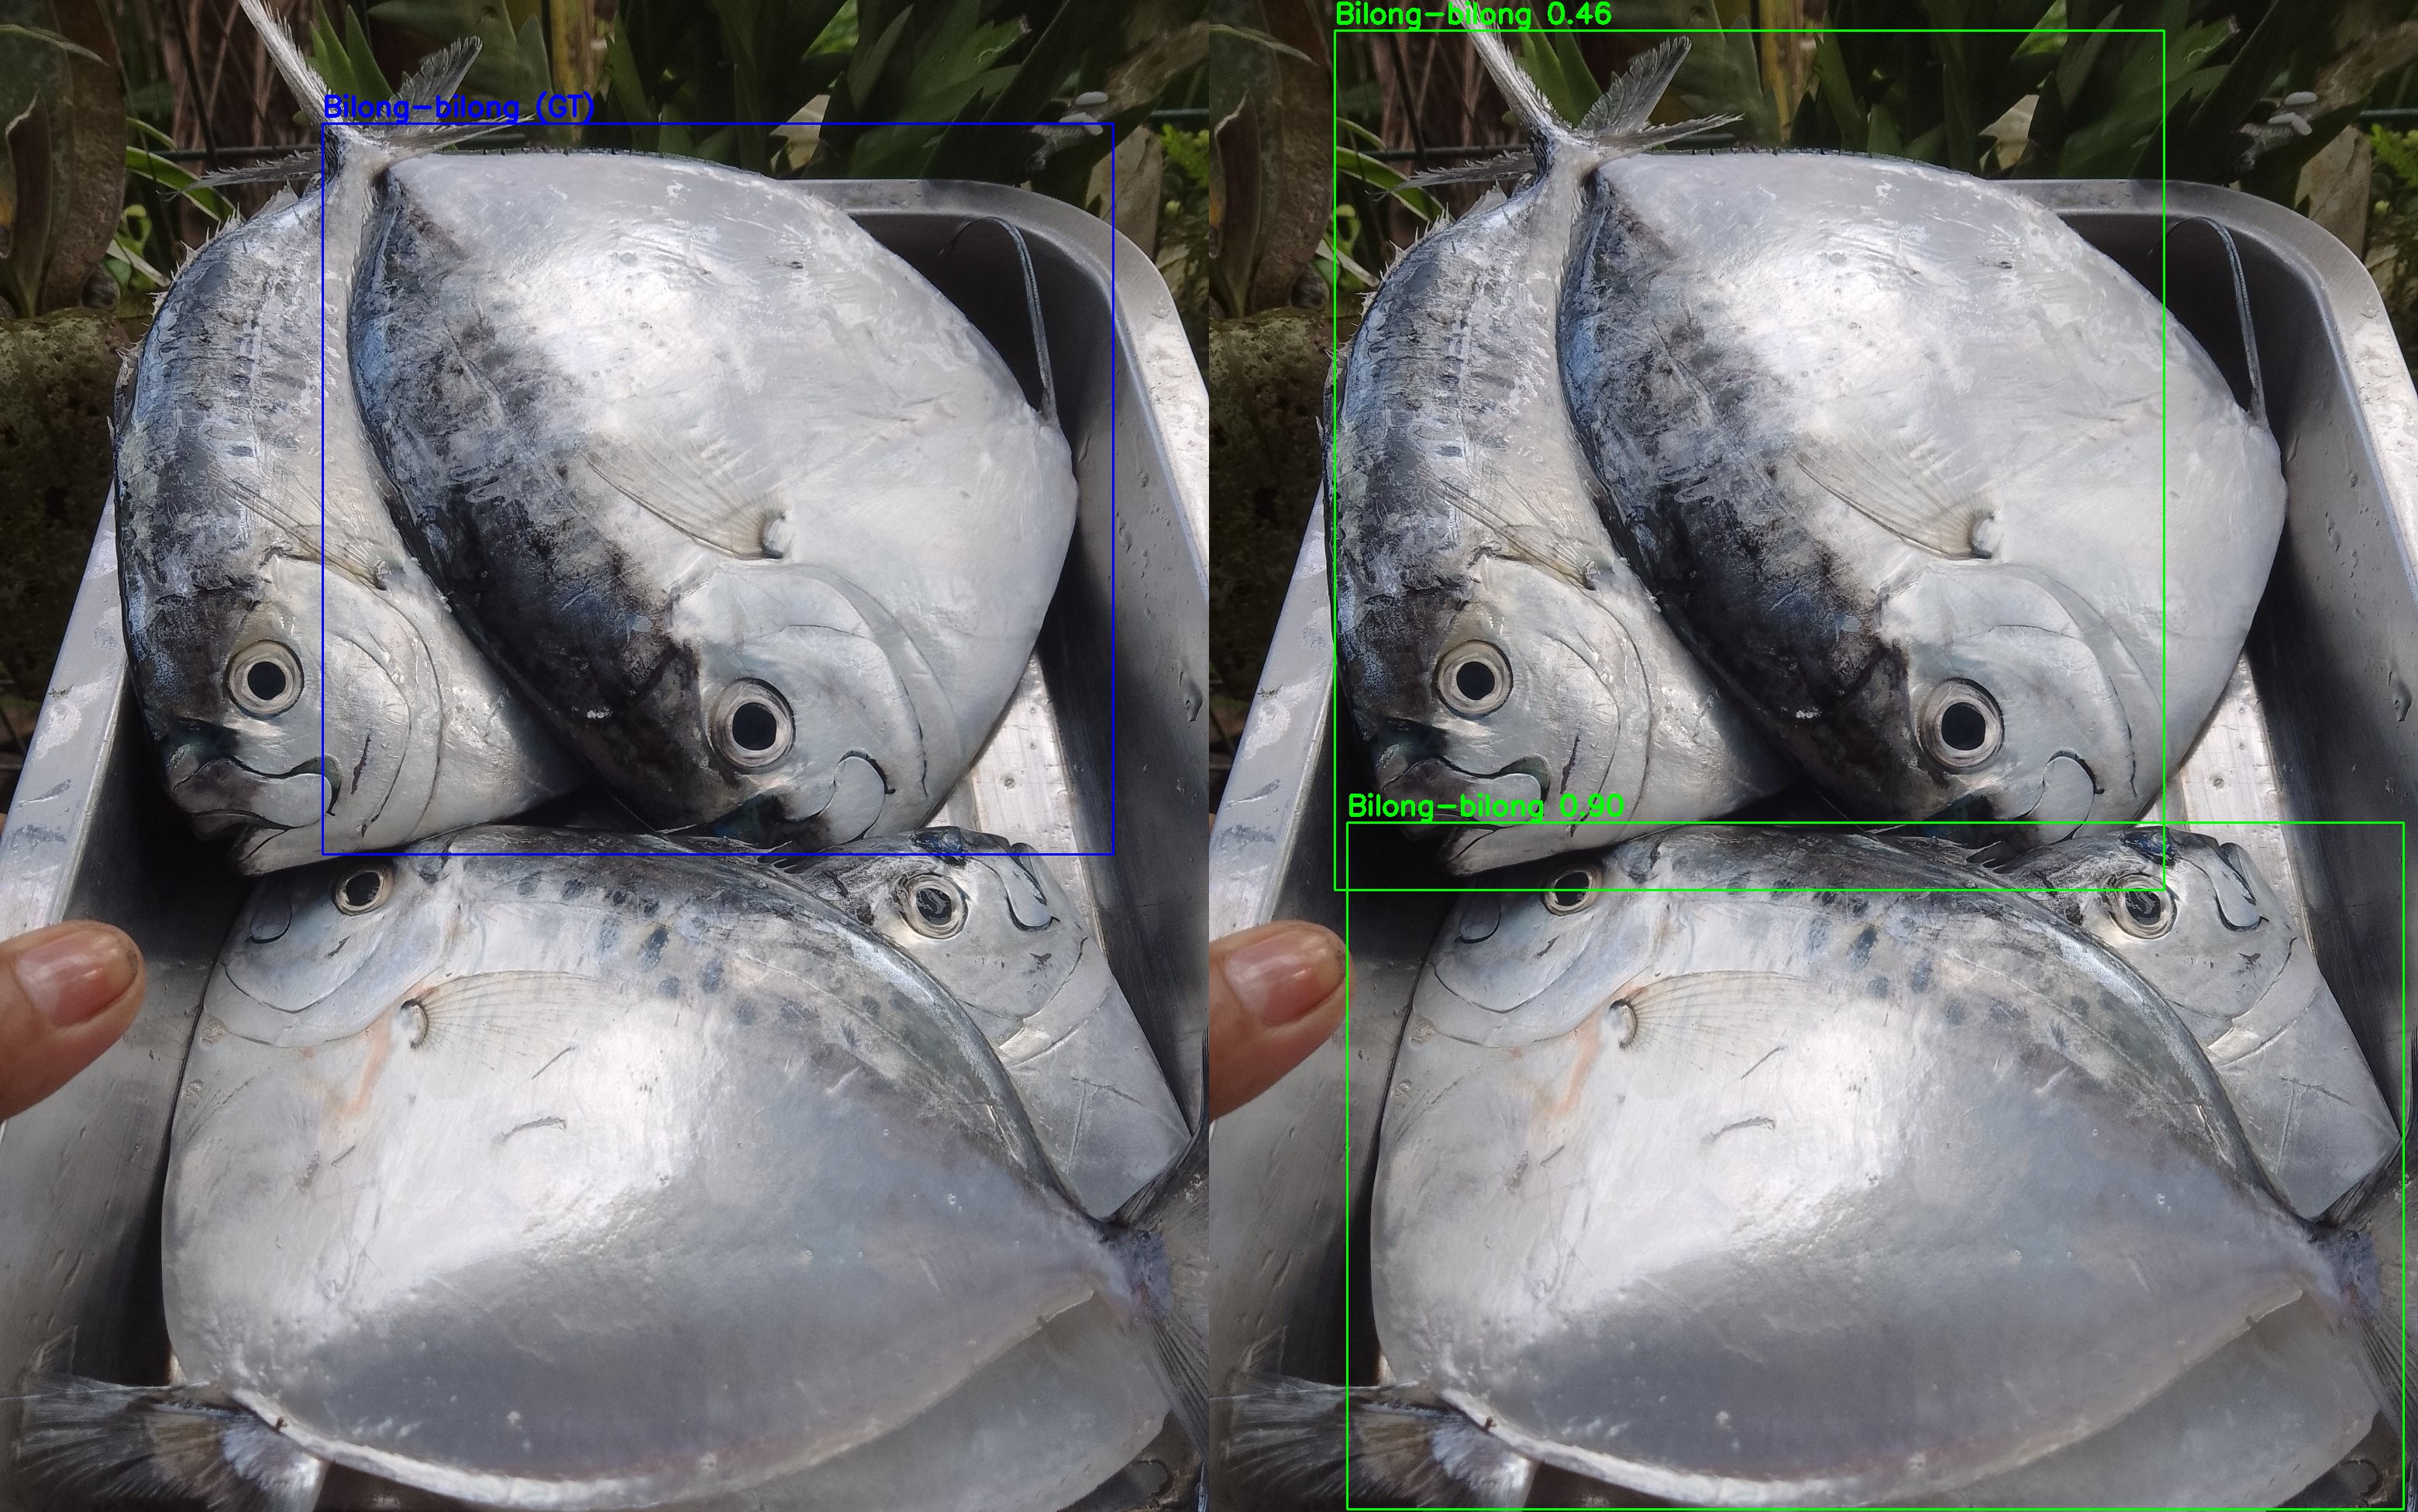
\includegraphics[width=0.8\textwidth]{images/images/predictions_per_class/Labeled_Bilong-bilong_Detected_Bilong-bilong.jpg}
    \caption{Ground Truth vs. Predicted Bounding Boxes for Bilong-bilong} 
    \label{fig: Bilong-bilong}
\end{figure}

\begin{figure}[H]
    \centering
    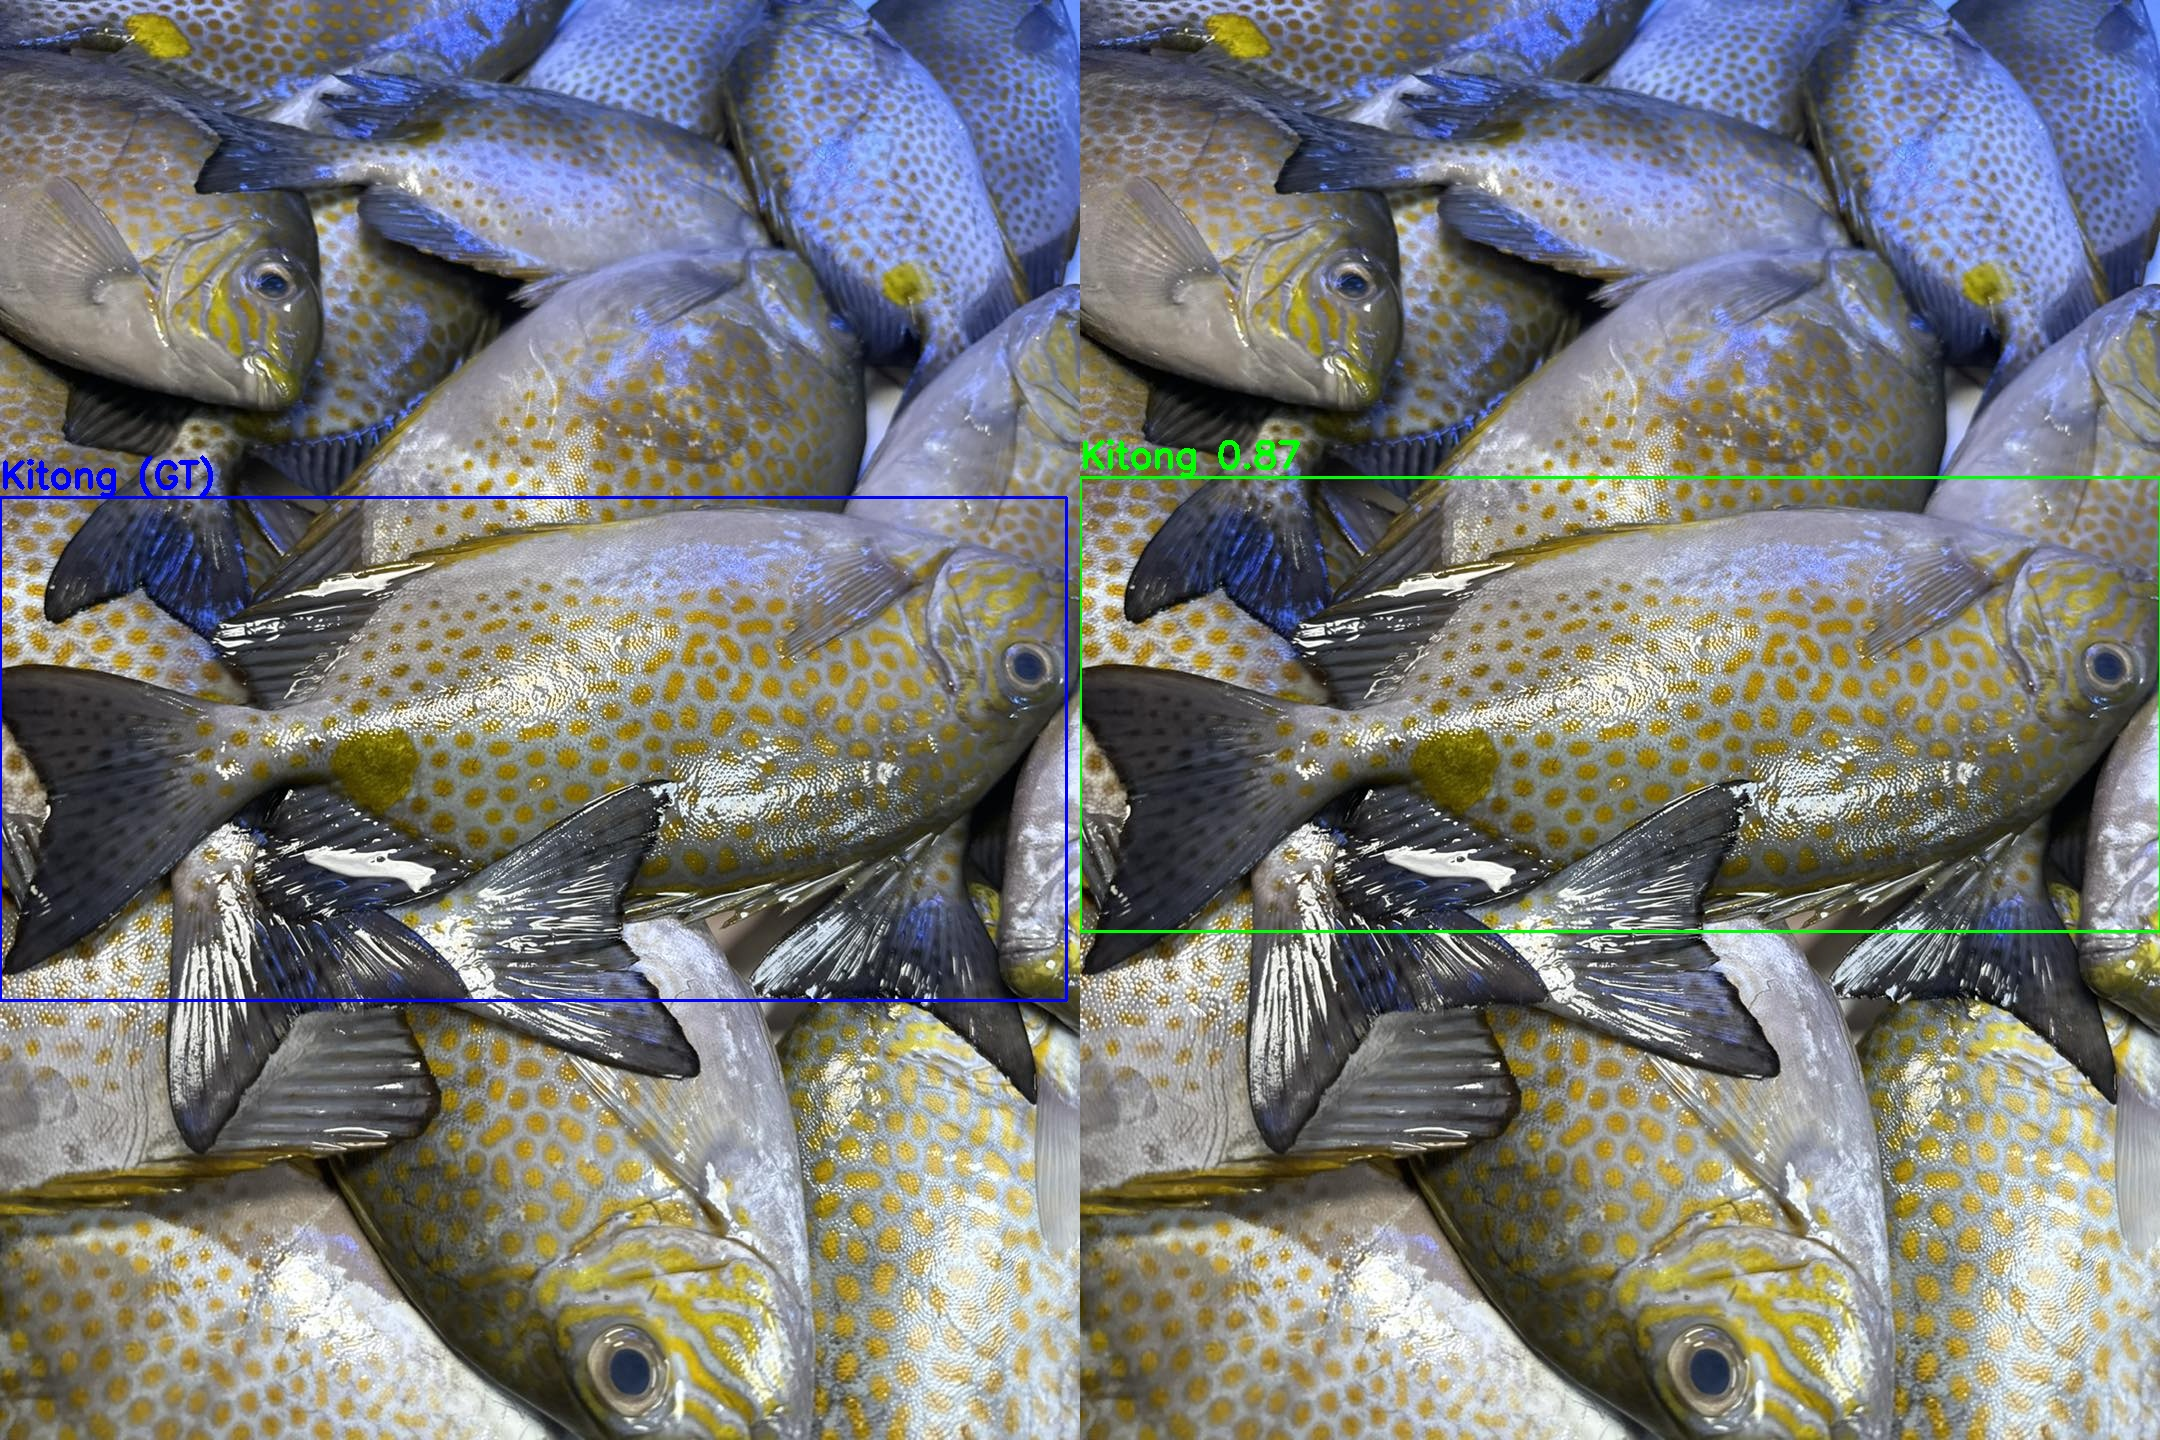
\includegraphics[width=0.8\textwidth]{images/images/predictions_per_class/Kitong_compare_6.jpg}
    \caption{Ground Truth vs. Predicted Bounding Boxes for Kitong} 
    \label{fig:Kitong}
\end{figure}

\begin{figure}[H]
    \centering
    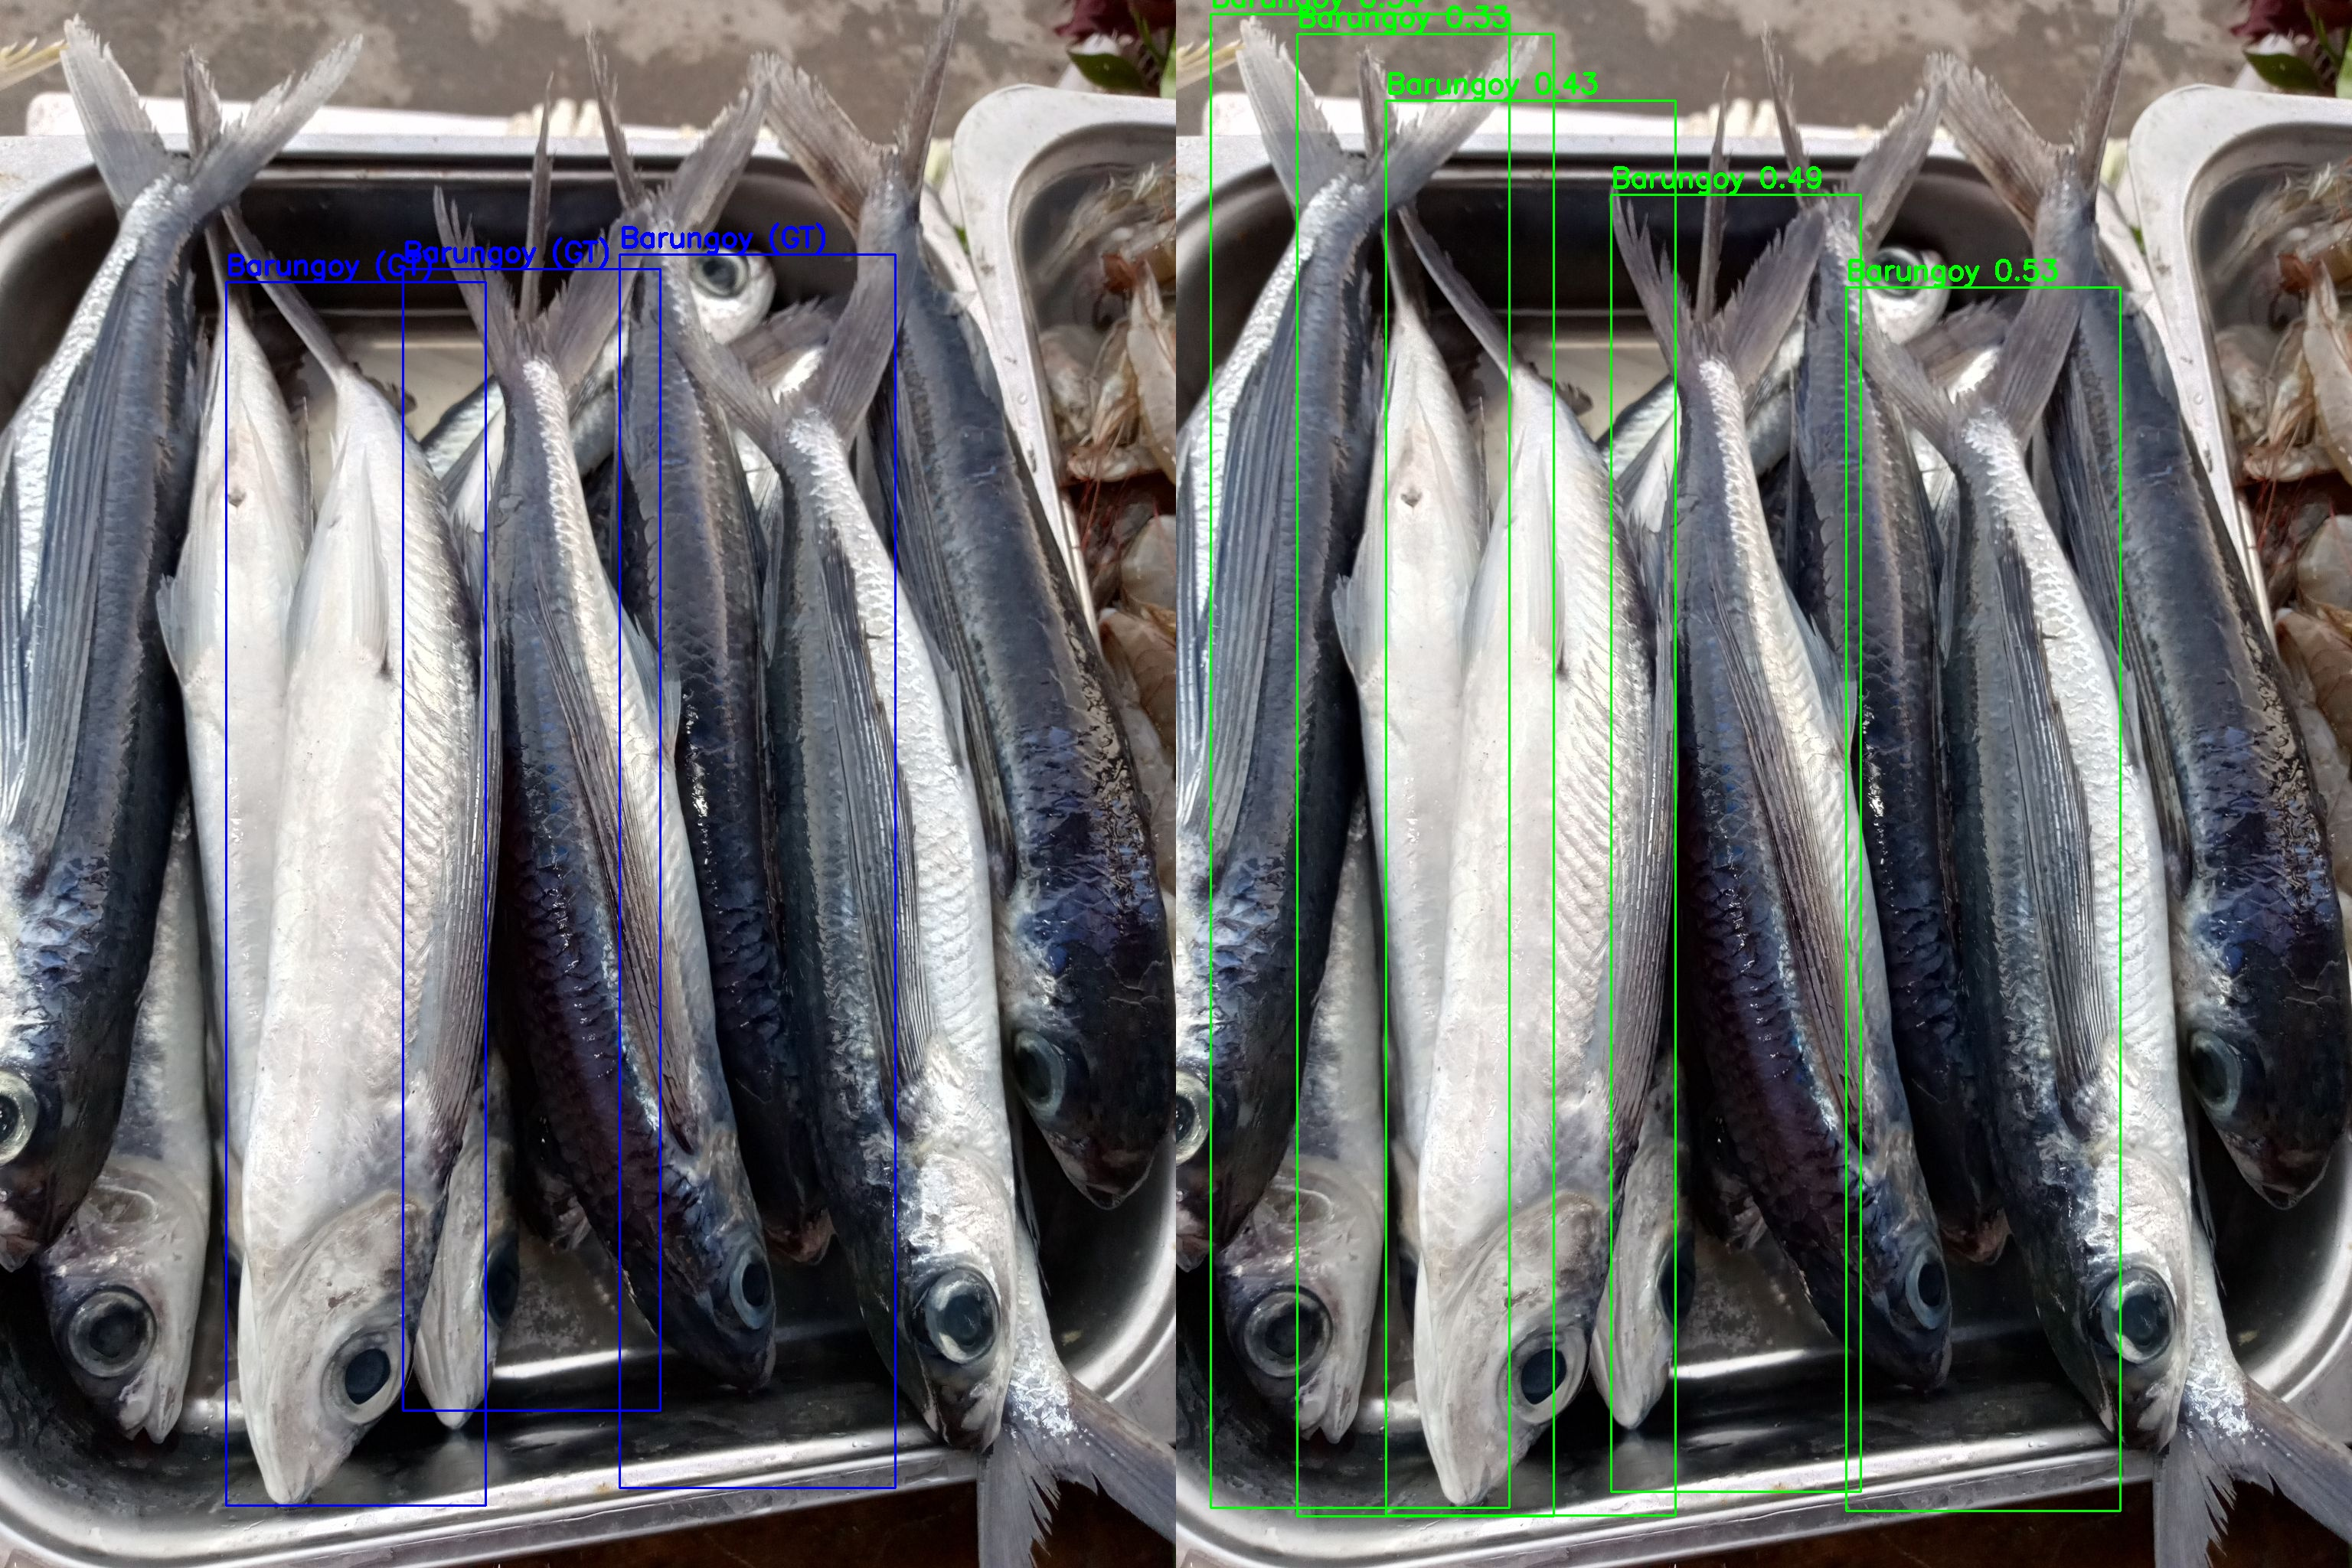
\includegraphics[width=0.8\textwidth]{images/images/predictions_per_class/Barungoy_compare_5.jpg}
    \caption{Ground Truth vs. Predicted Bounding Boxes for Barungoy} 
    \label{fig: Barungoy}
\end{figure}

\begin{figure}[H]
    \centering
    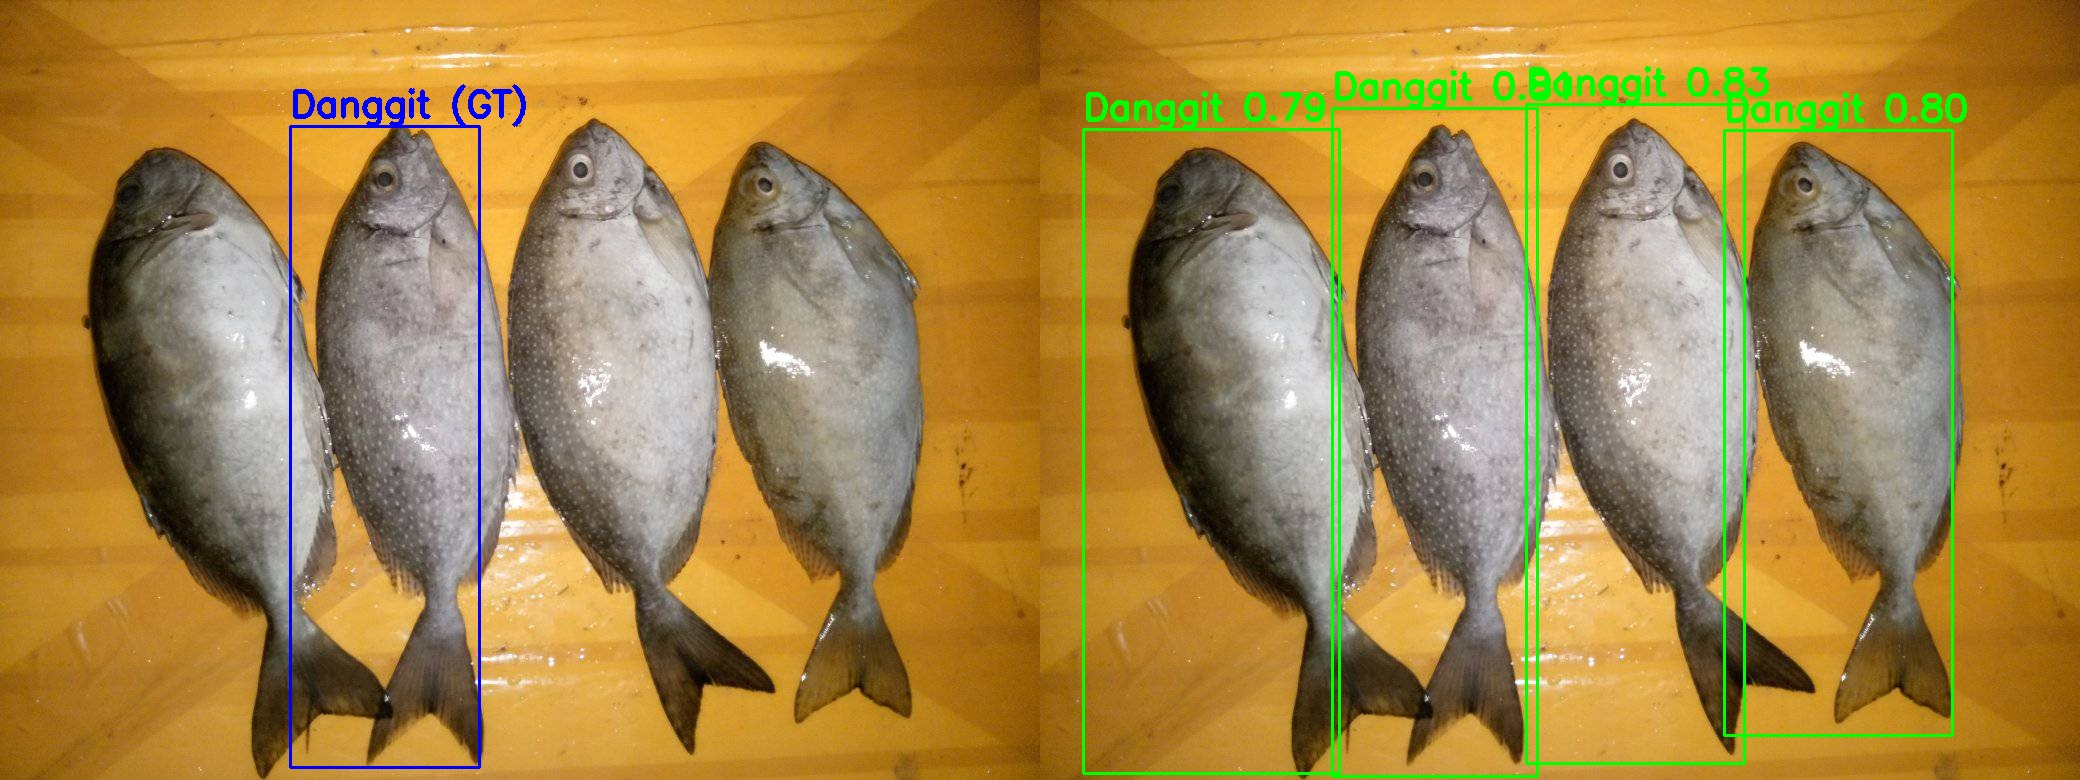
\includegraphics[width=0.8\textwidth]{images/images/predictions_per_class/Labeled_Danggit_Detected_Danggit.jpg}
    \caption{Ground Truth vs. Predicted Bounding Boxes for Danggit} 
    \label{fig: Danggit}
\end{figure}

\begin{figure}[H]
    \centering
    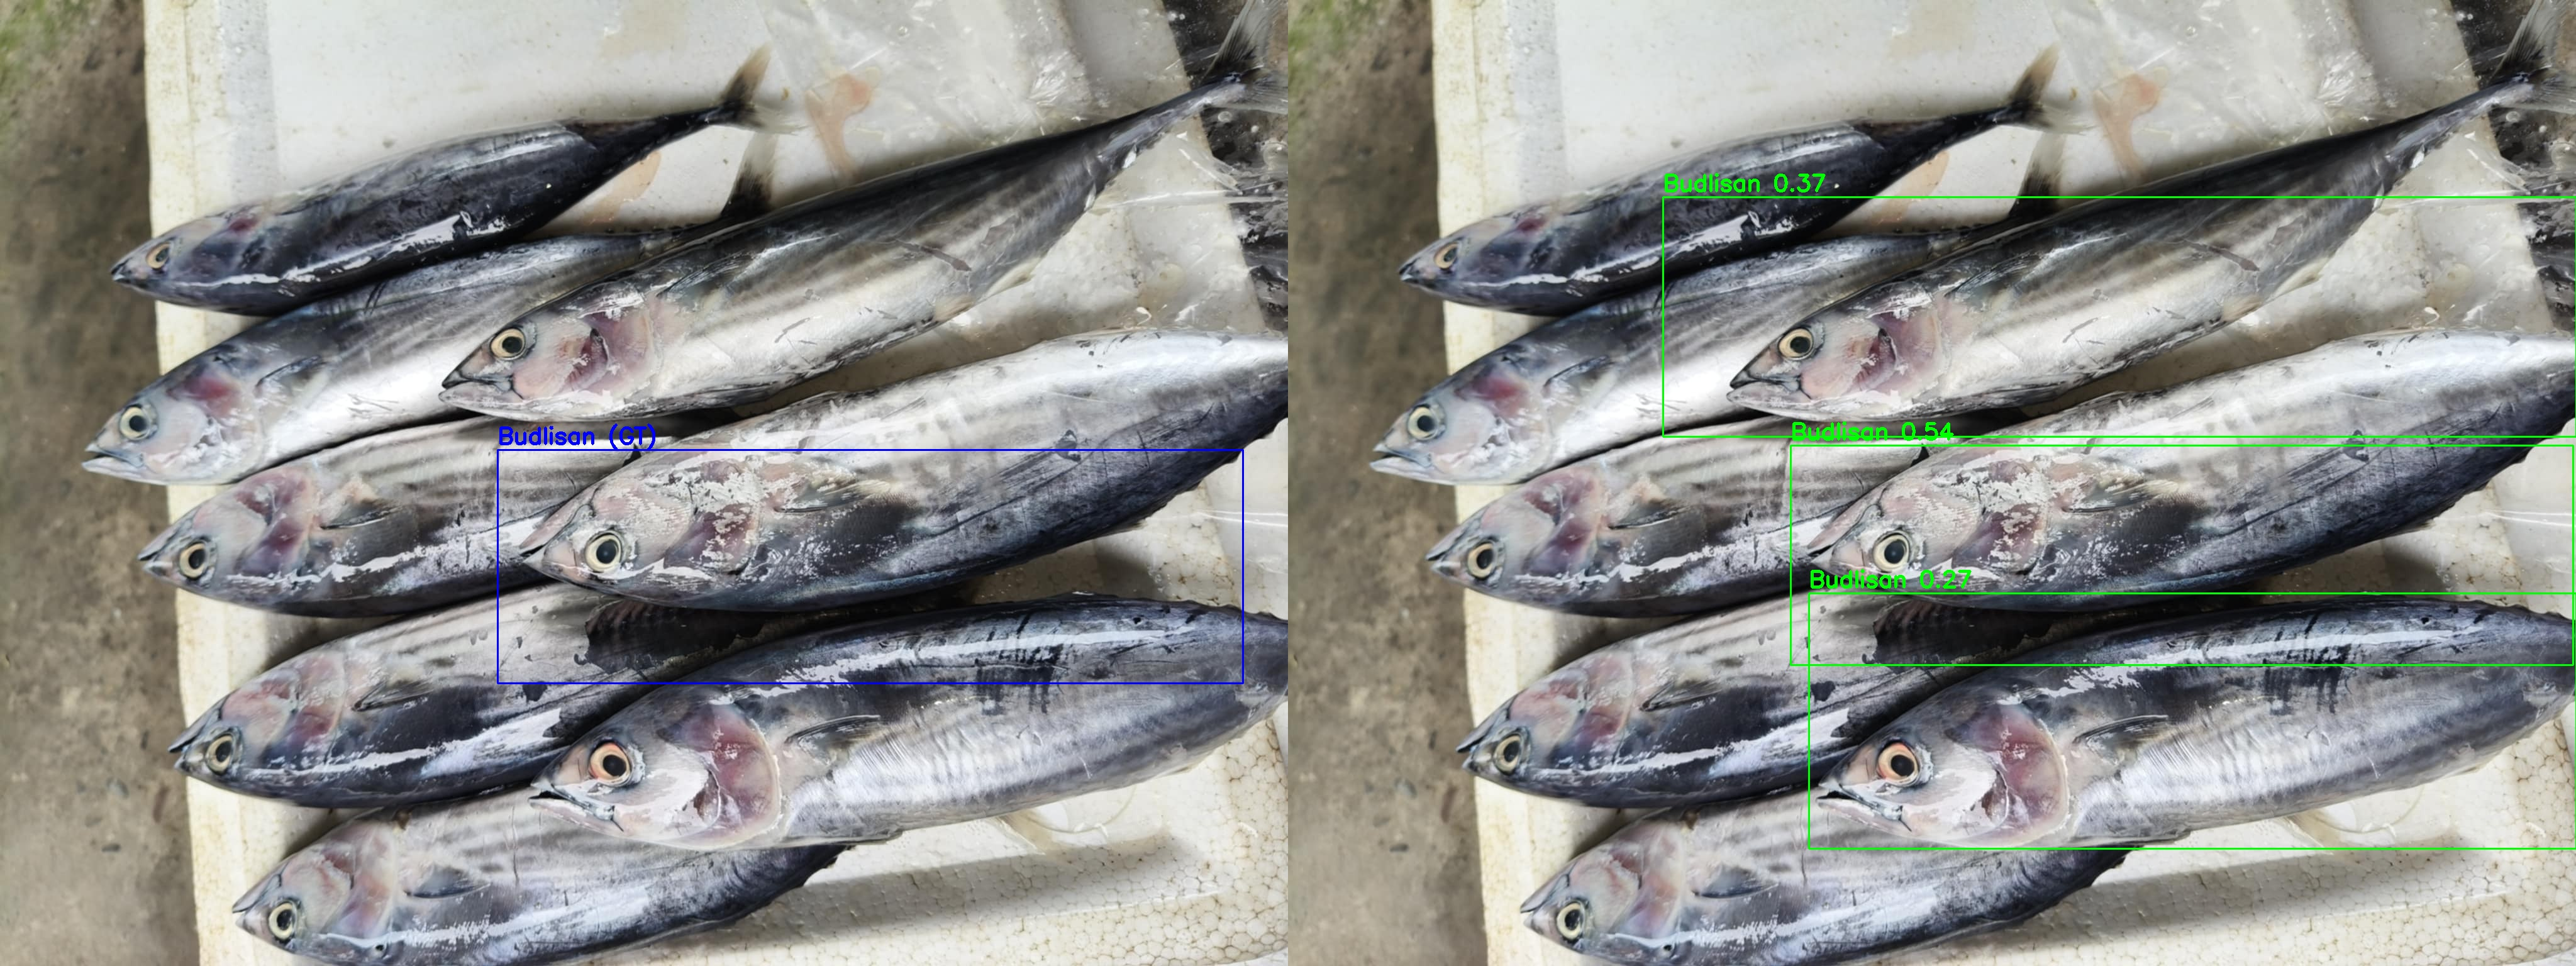
\includegraphics[width=0.8\textwidth]{images/images/predictions_per_class/Labeled_Budlisan_Detected_Budlisan.jpg}
    \caption{Ground Truth vs. Predicted Bounding Boxes for Budlisan} 
    \label{fig:Budlisan}
\end{figure}

\begin{figure}[H]
    \centering
    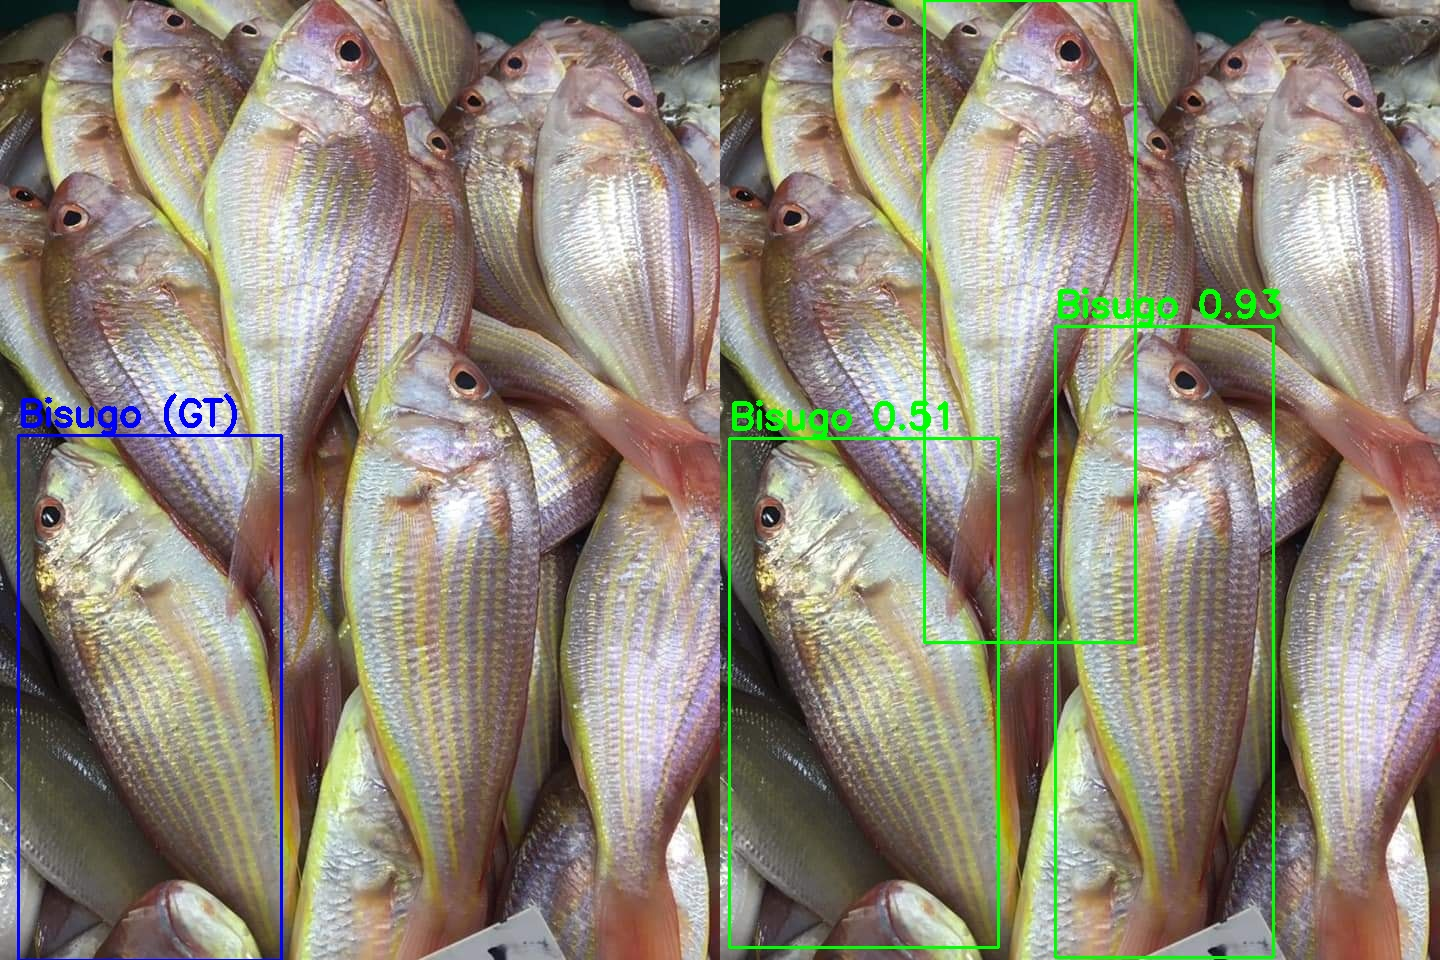
\includegraphics[width=0.8\textwidth]{images/images/predictions_per_class/Labeled_Bisugo_Detected_Bisugo.jpg}
    \caption{Ground Truth vs. Predicted Bounding Boxes for Bisugo} 
    \label{fig: Bisugo}
\end{figure}


\begin{figure}[H]
    \centering
    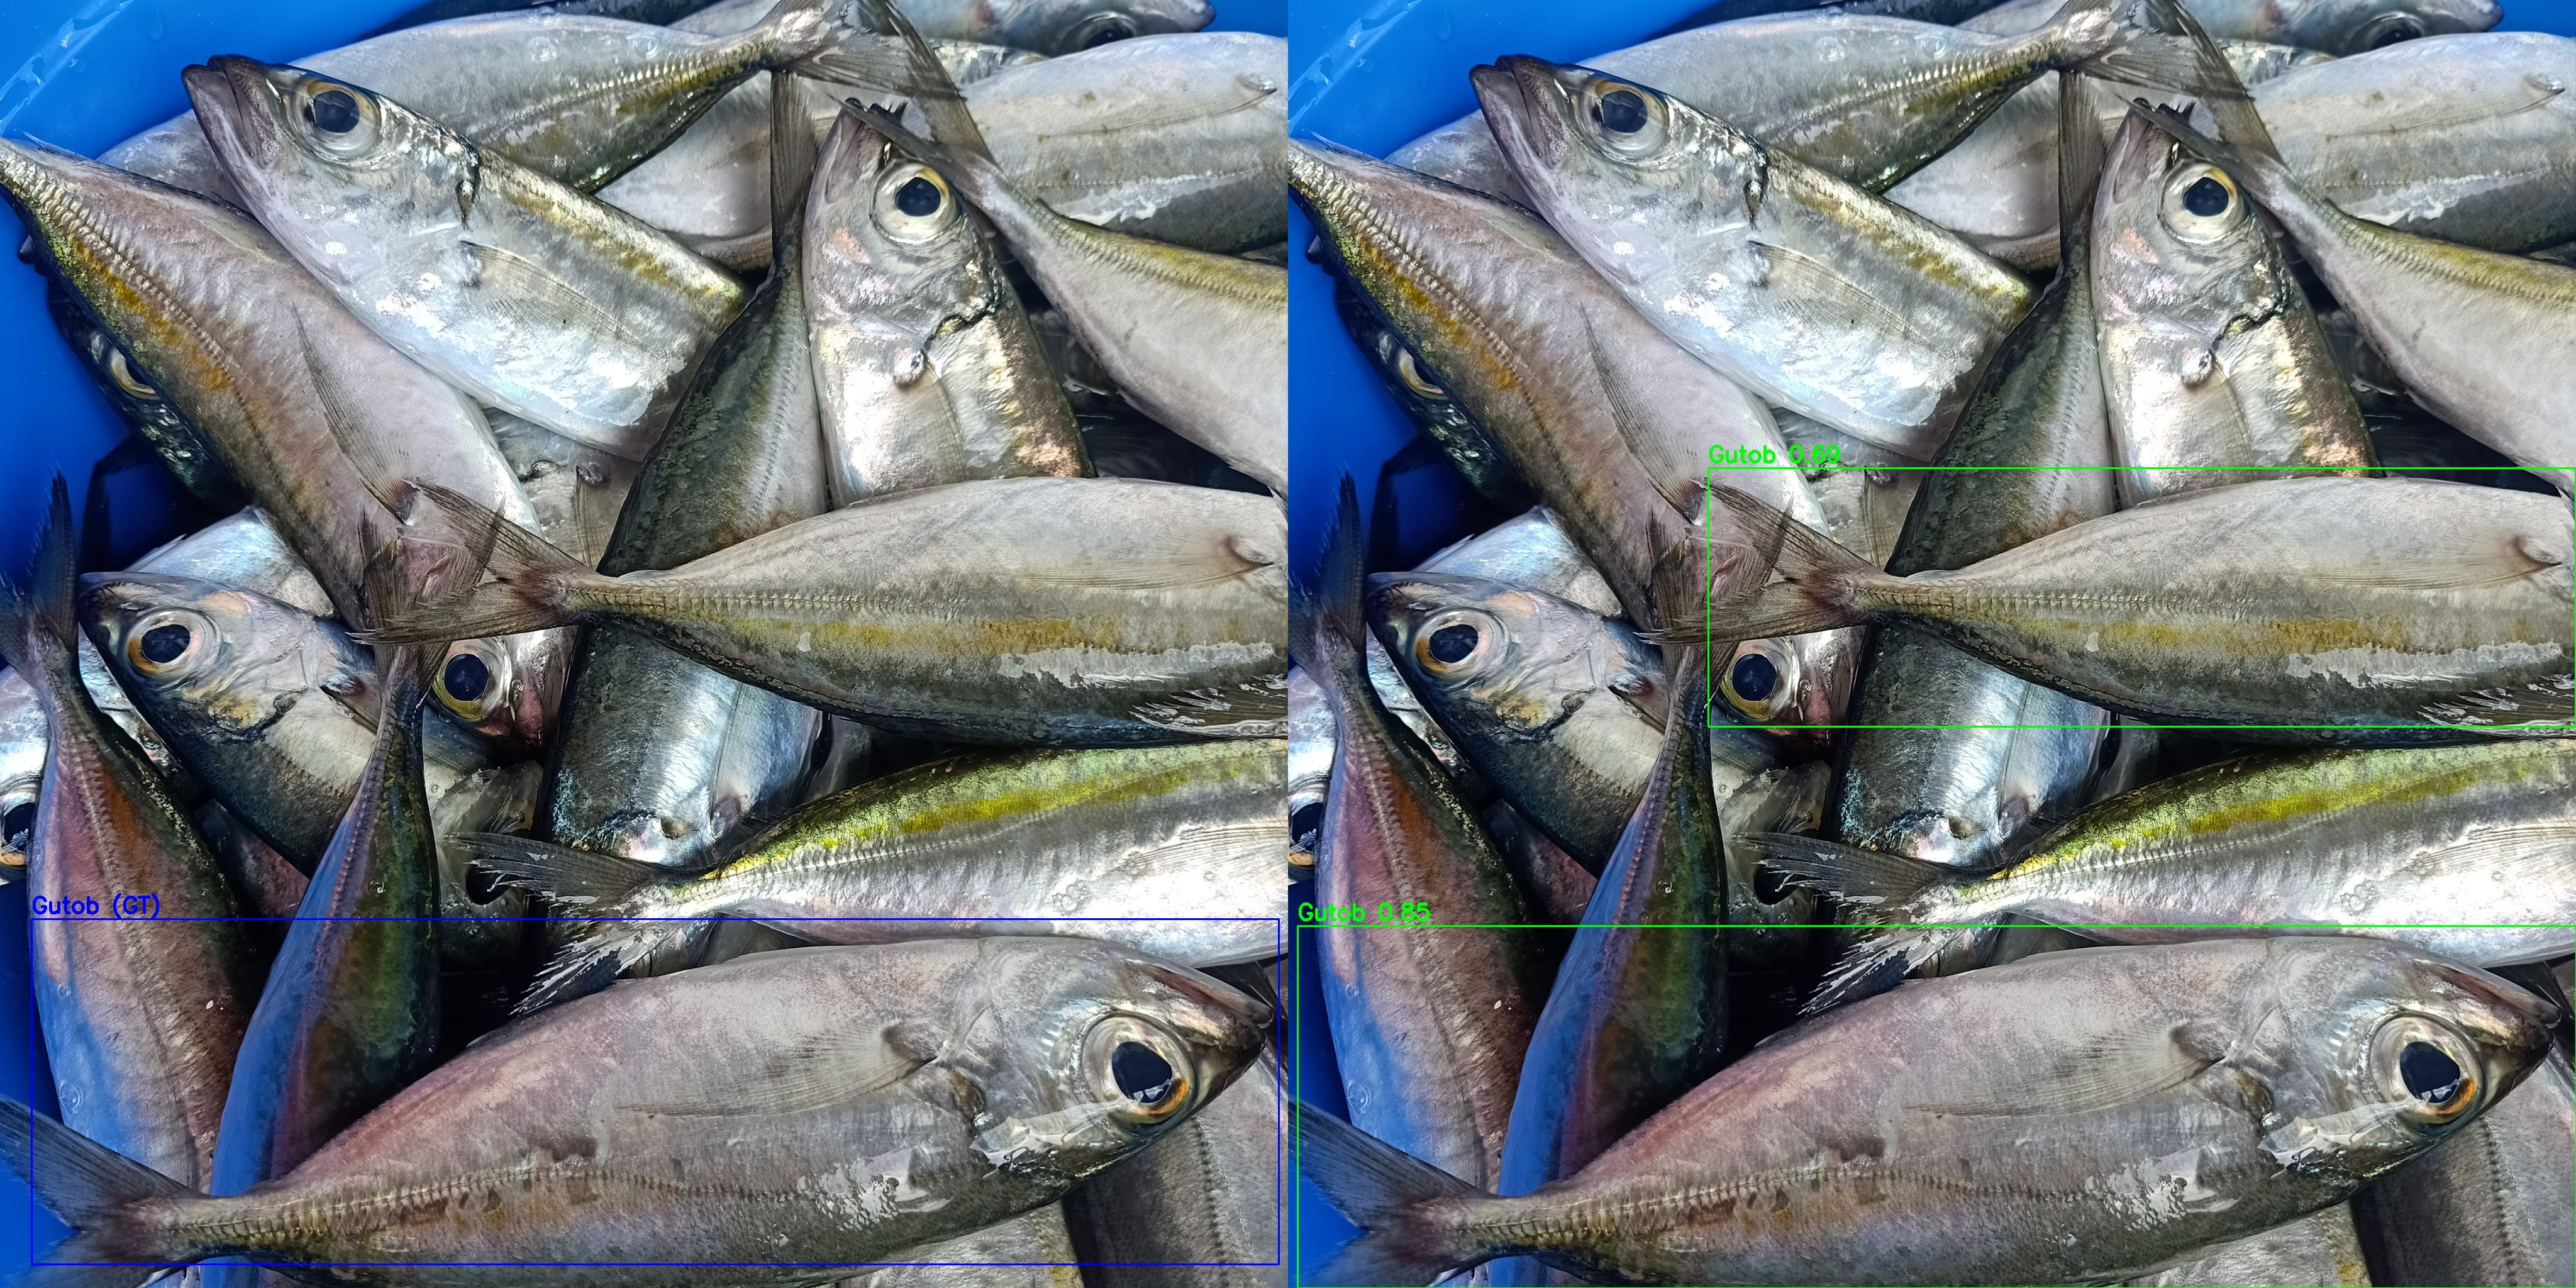
\includegraphics[width=0.8\textwidth]{images/images/predictions_per_class/Gutob_compare_8.jpg}
    \caption{Ground Truth vs. Predicted Bounding Boxes for Gutob} 
    \label{fig: Gutob}
\end{figure}

\begin{figure}[H]
    \centering
    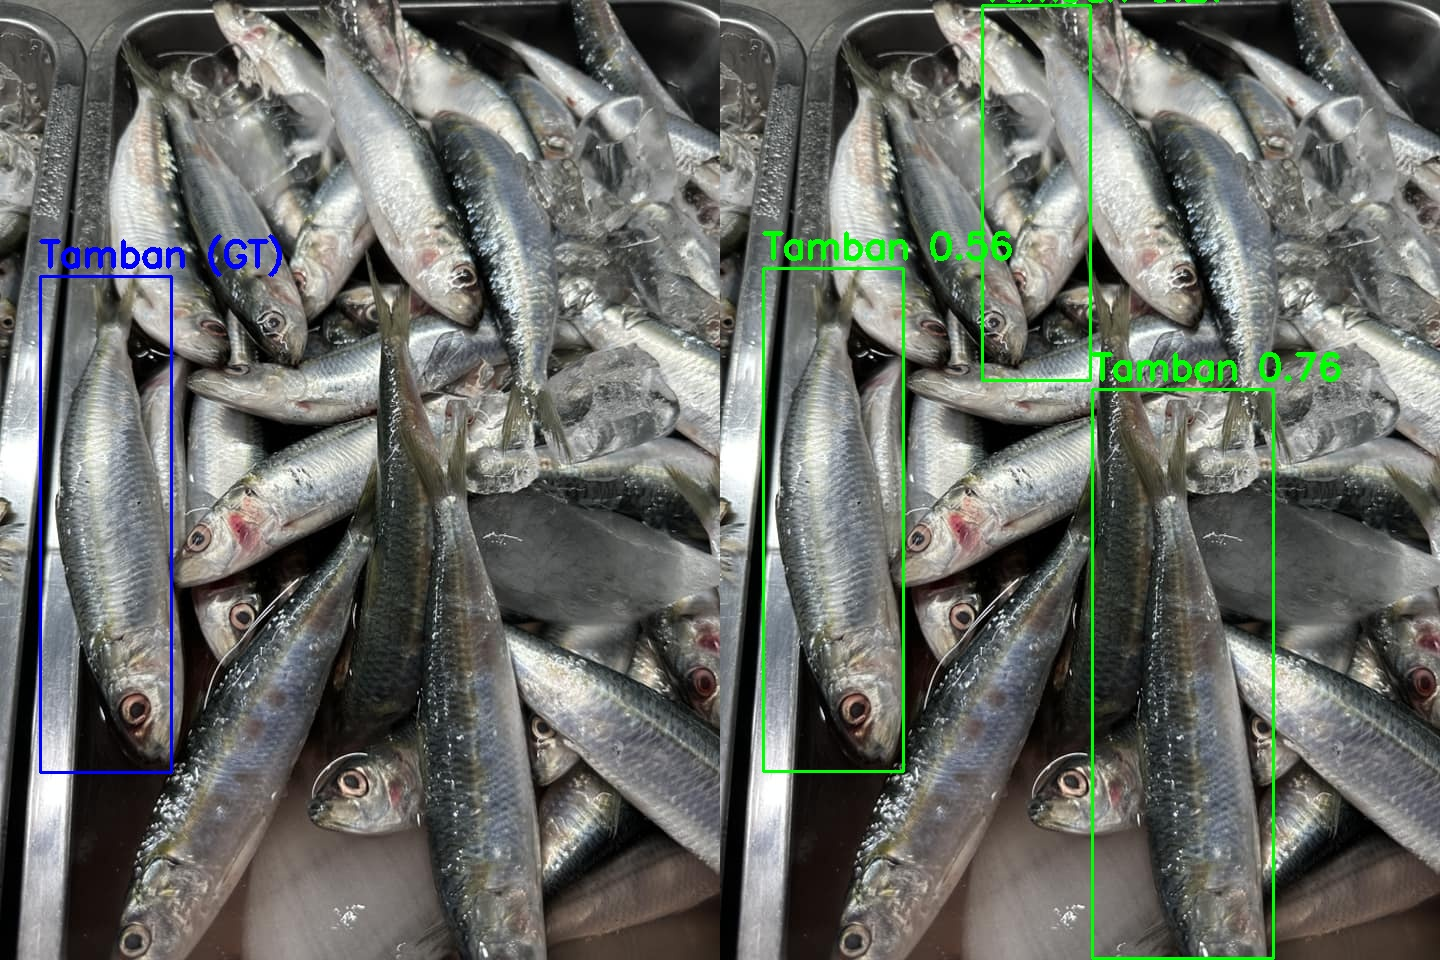
\includegraphics[width=0.8\textwidth]{images/images/predictions_per_class/Tamban_compare_19.jpg}
    \caption{Ground Truth vs. Predicted Bounding Boxes for Tamban} 
    \label{fig:Tamban}
\end{figure}

\begin{figure}[H]
    \centering
    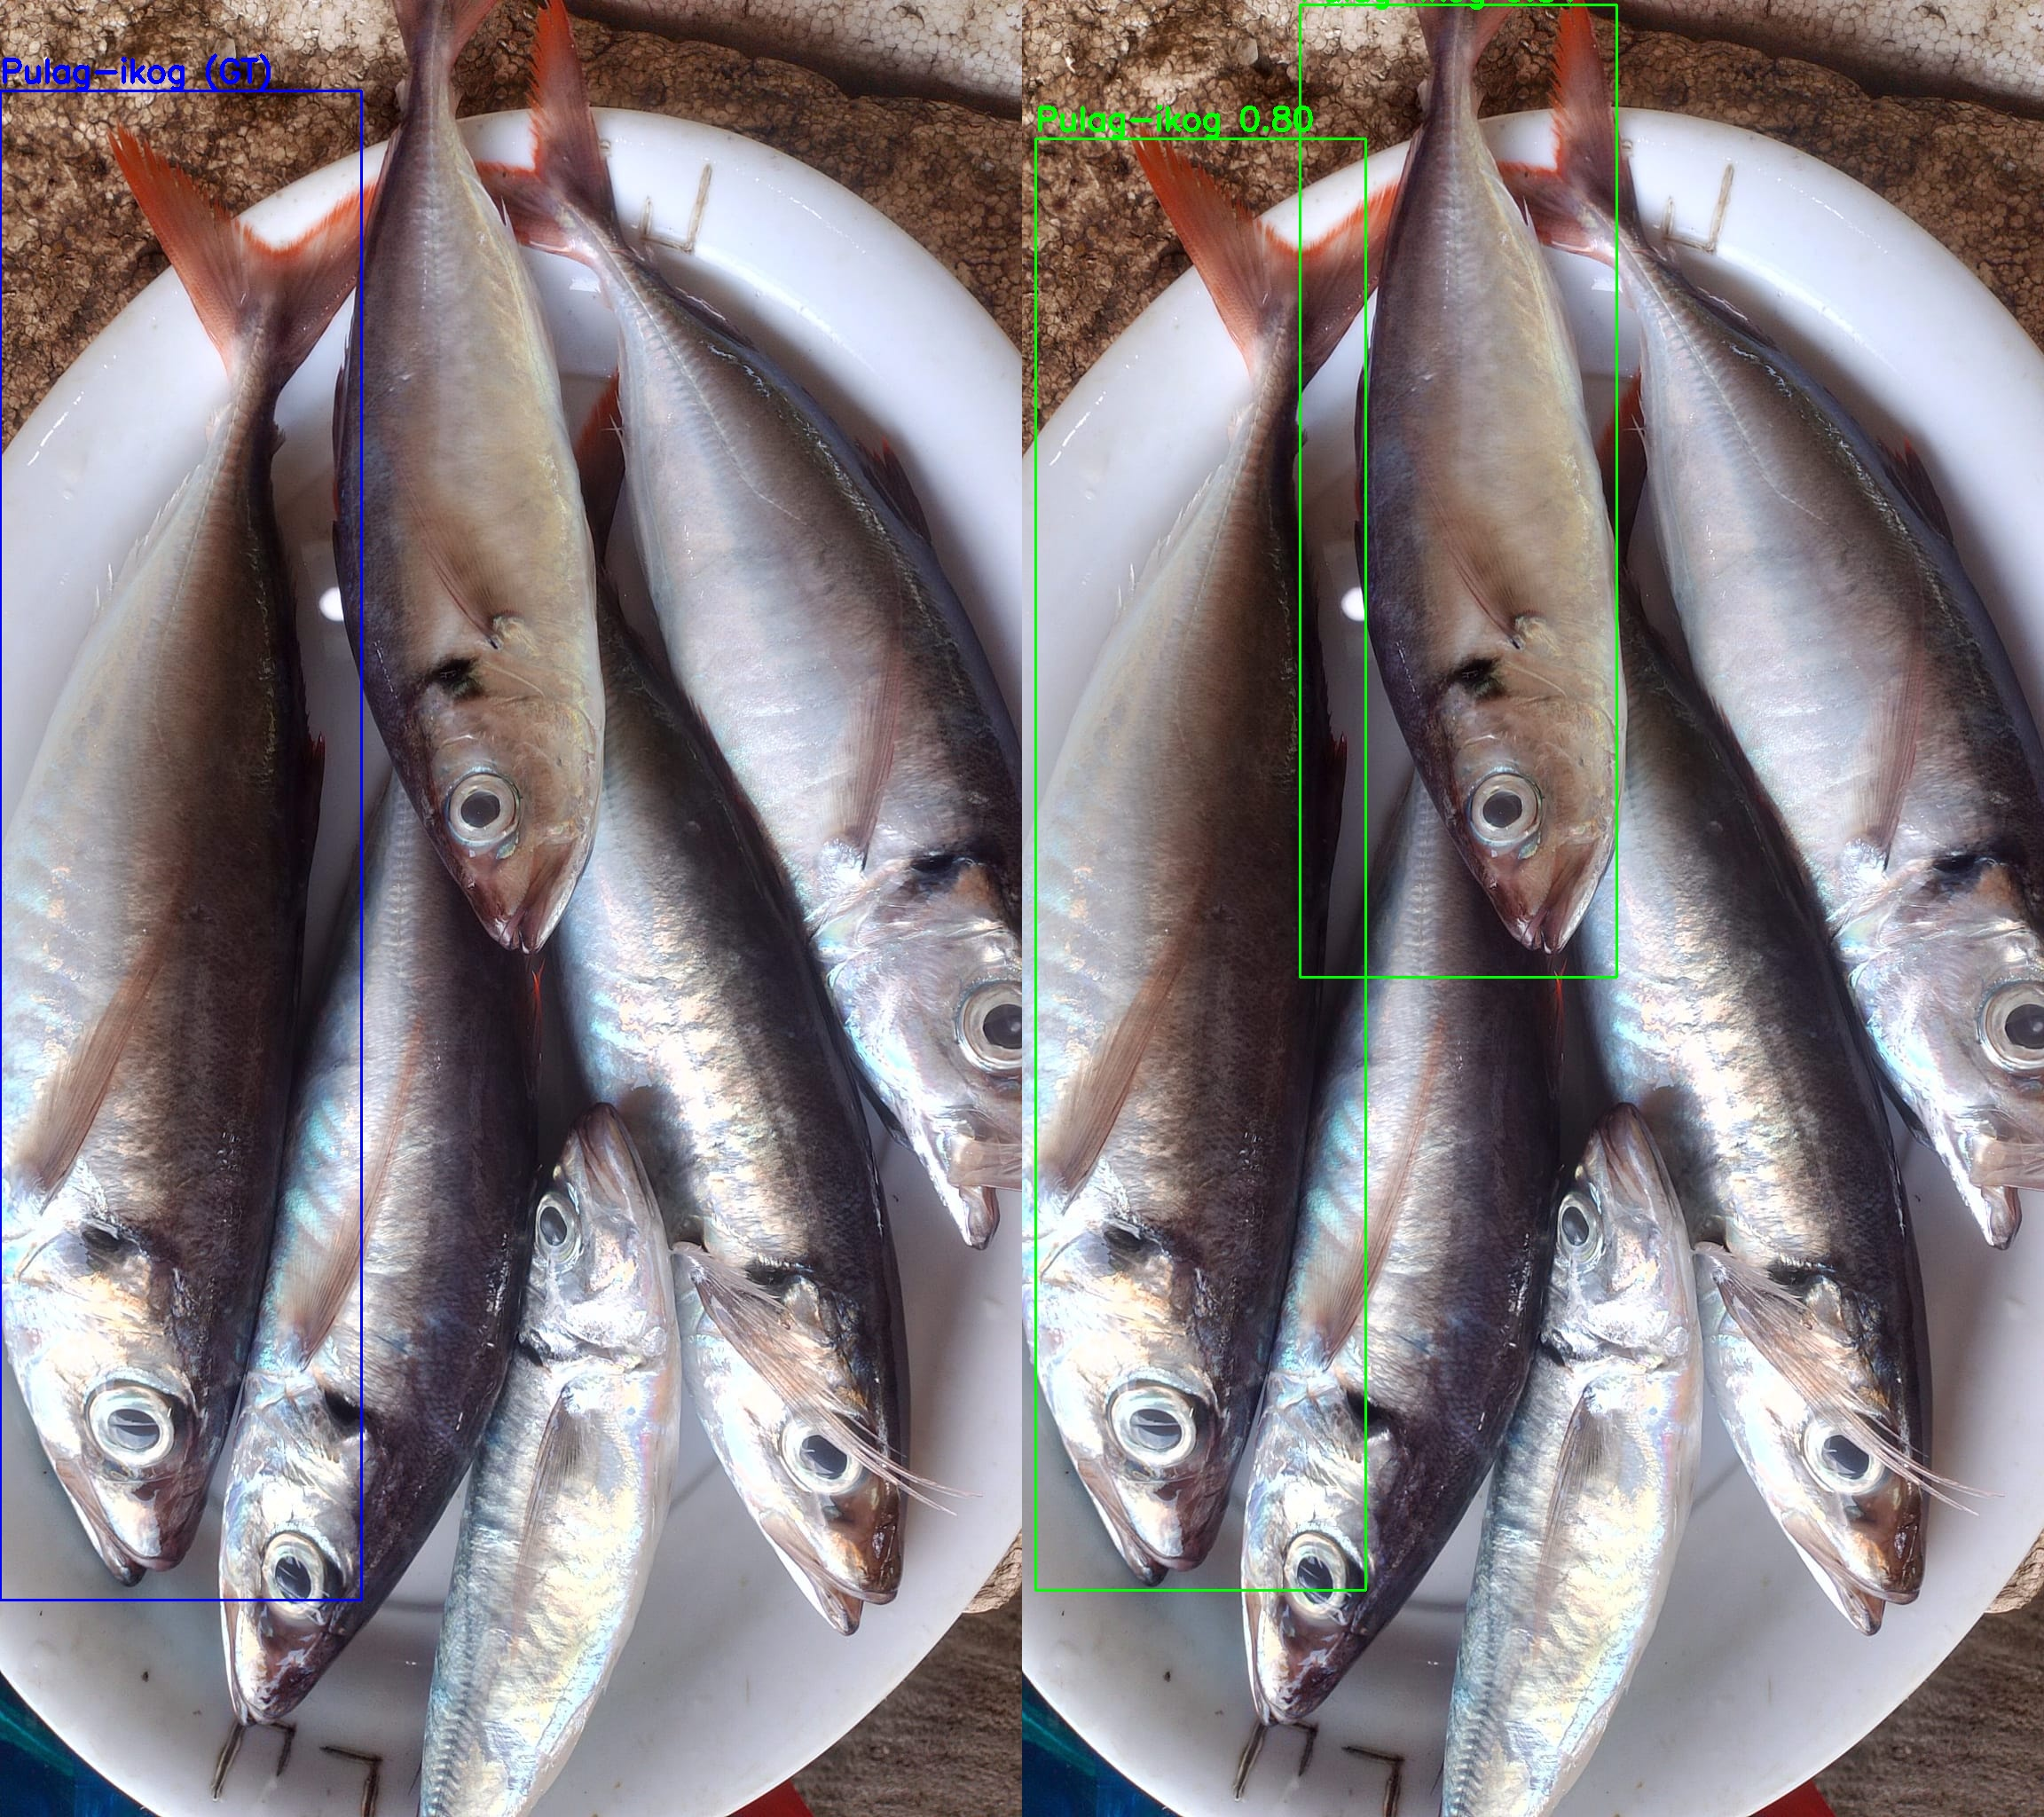
\includegraphics[width=0.8\textwidth]{images/images/predictions_per_class/Pulag-ikog_compare_6.jpg}
    \caption{Ground Truth vs. Predicted Bounding Boxes for Pulag-ikog} 
    \label{fig:Pulag-ikog}
\end{figure} 

\begin{figure}[H]
    \centering
    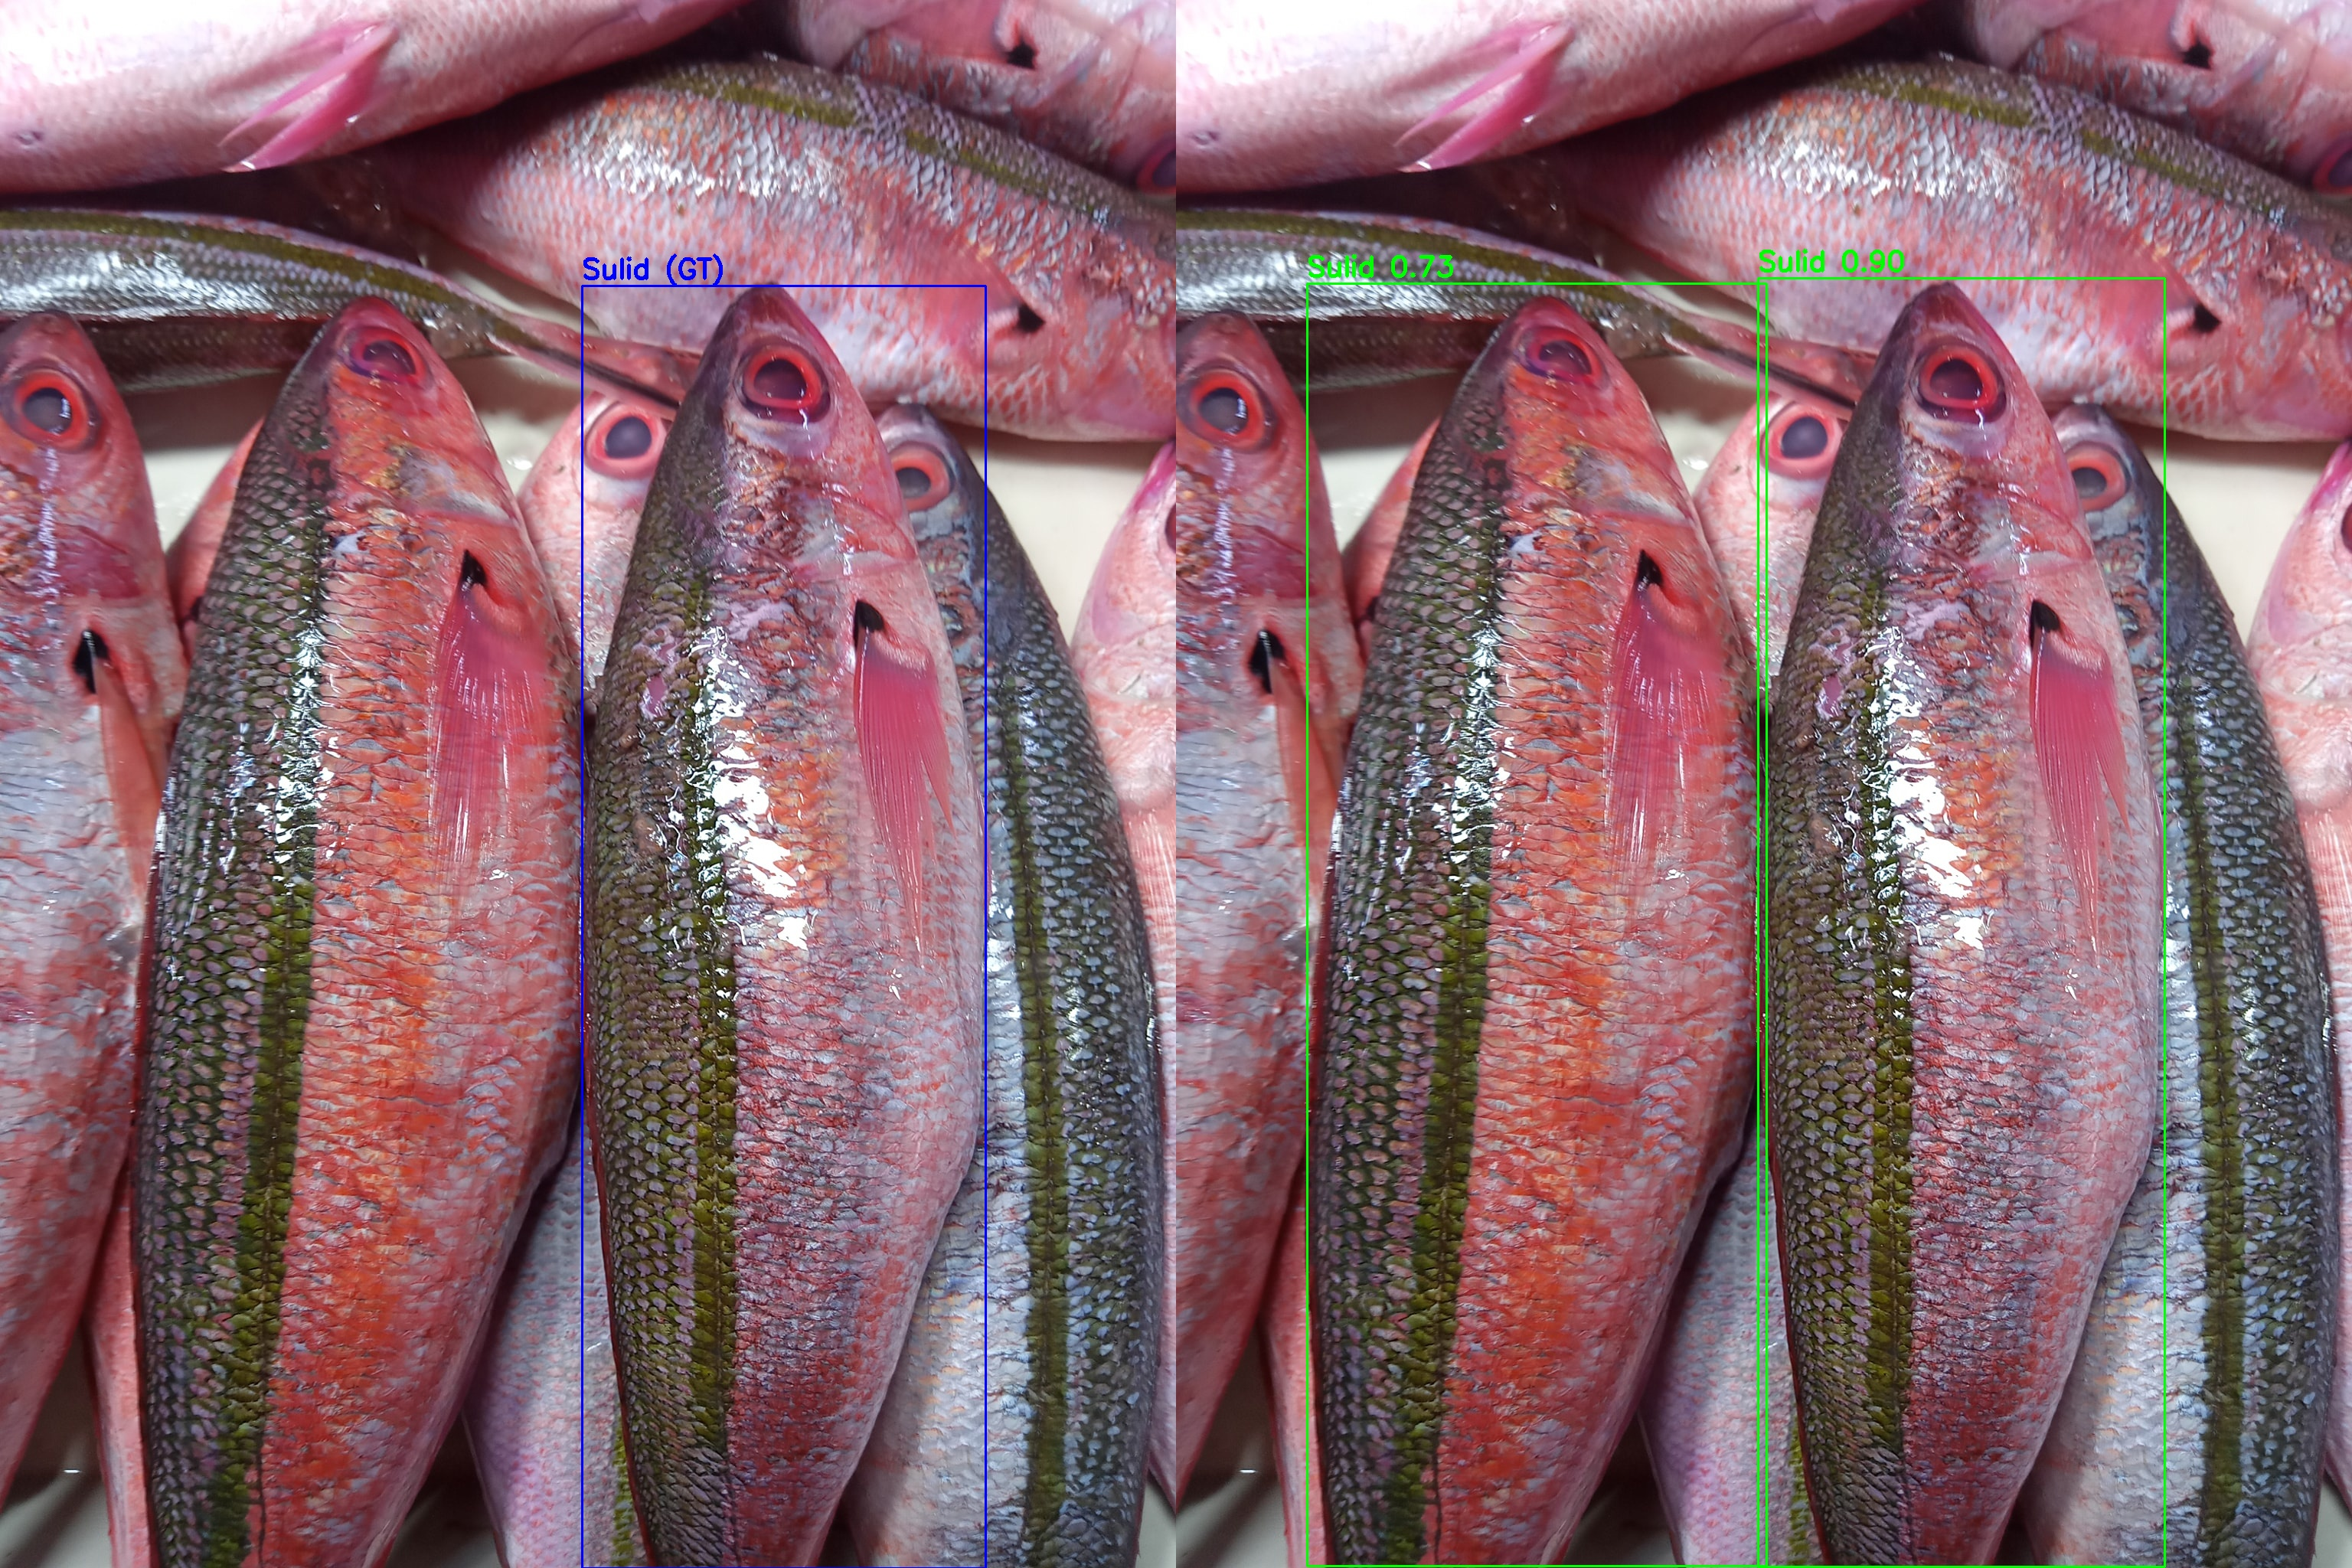
\includegraphics[width=0.8\textwidth]{images/images/predictions_per_class/Labeled_Sulid_Detected_Sulid.jpg}
    \caption{Ground Truth vs. Predicted Bounding Boxes for Sulid} 
    \label{fig:Sulid}
\end{figure} 

\begin{figure}[H]
    \centering
    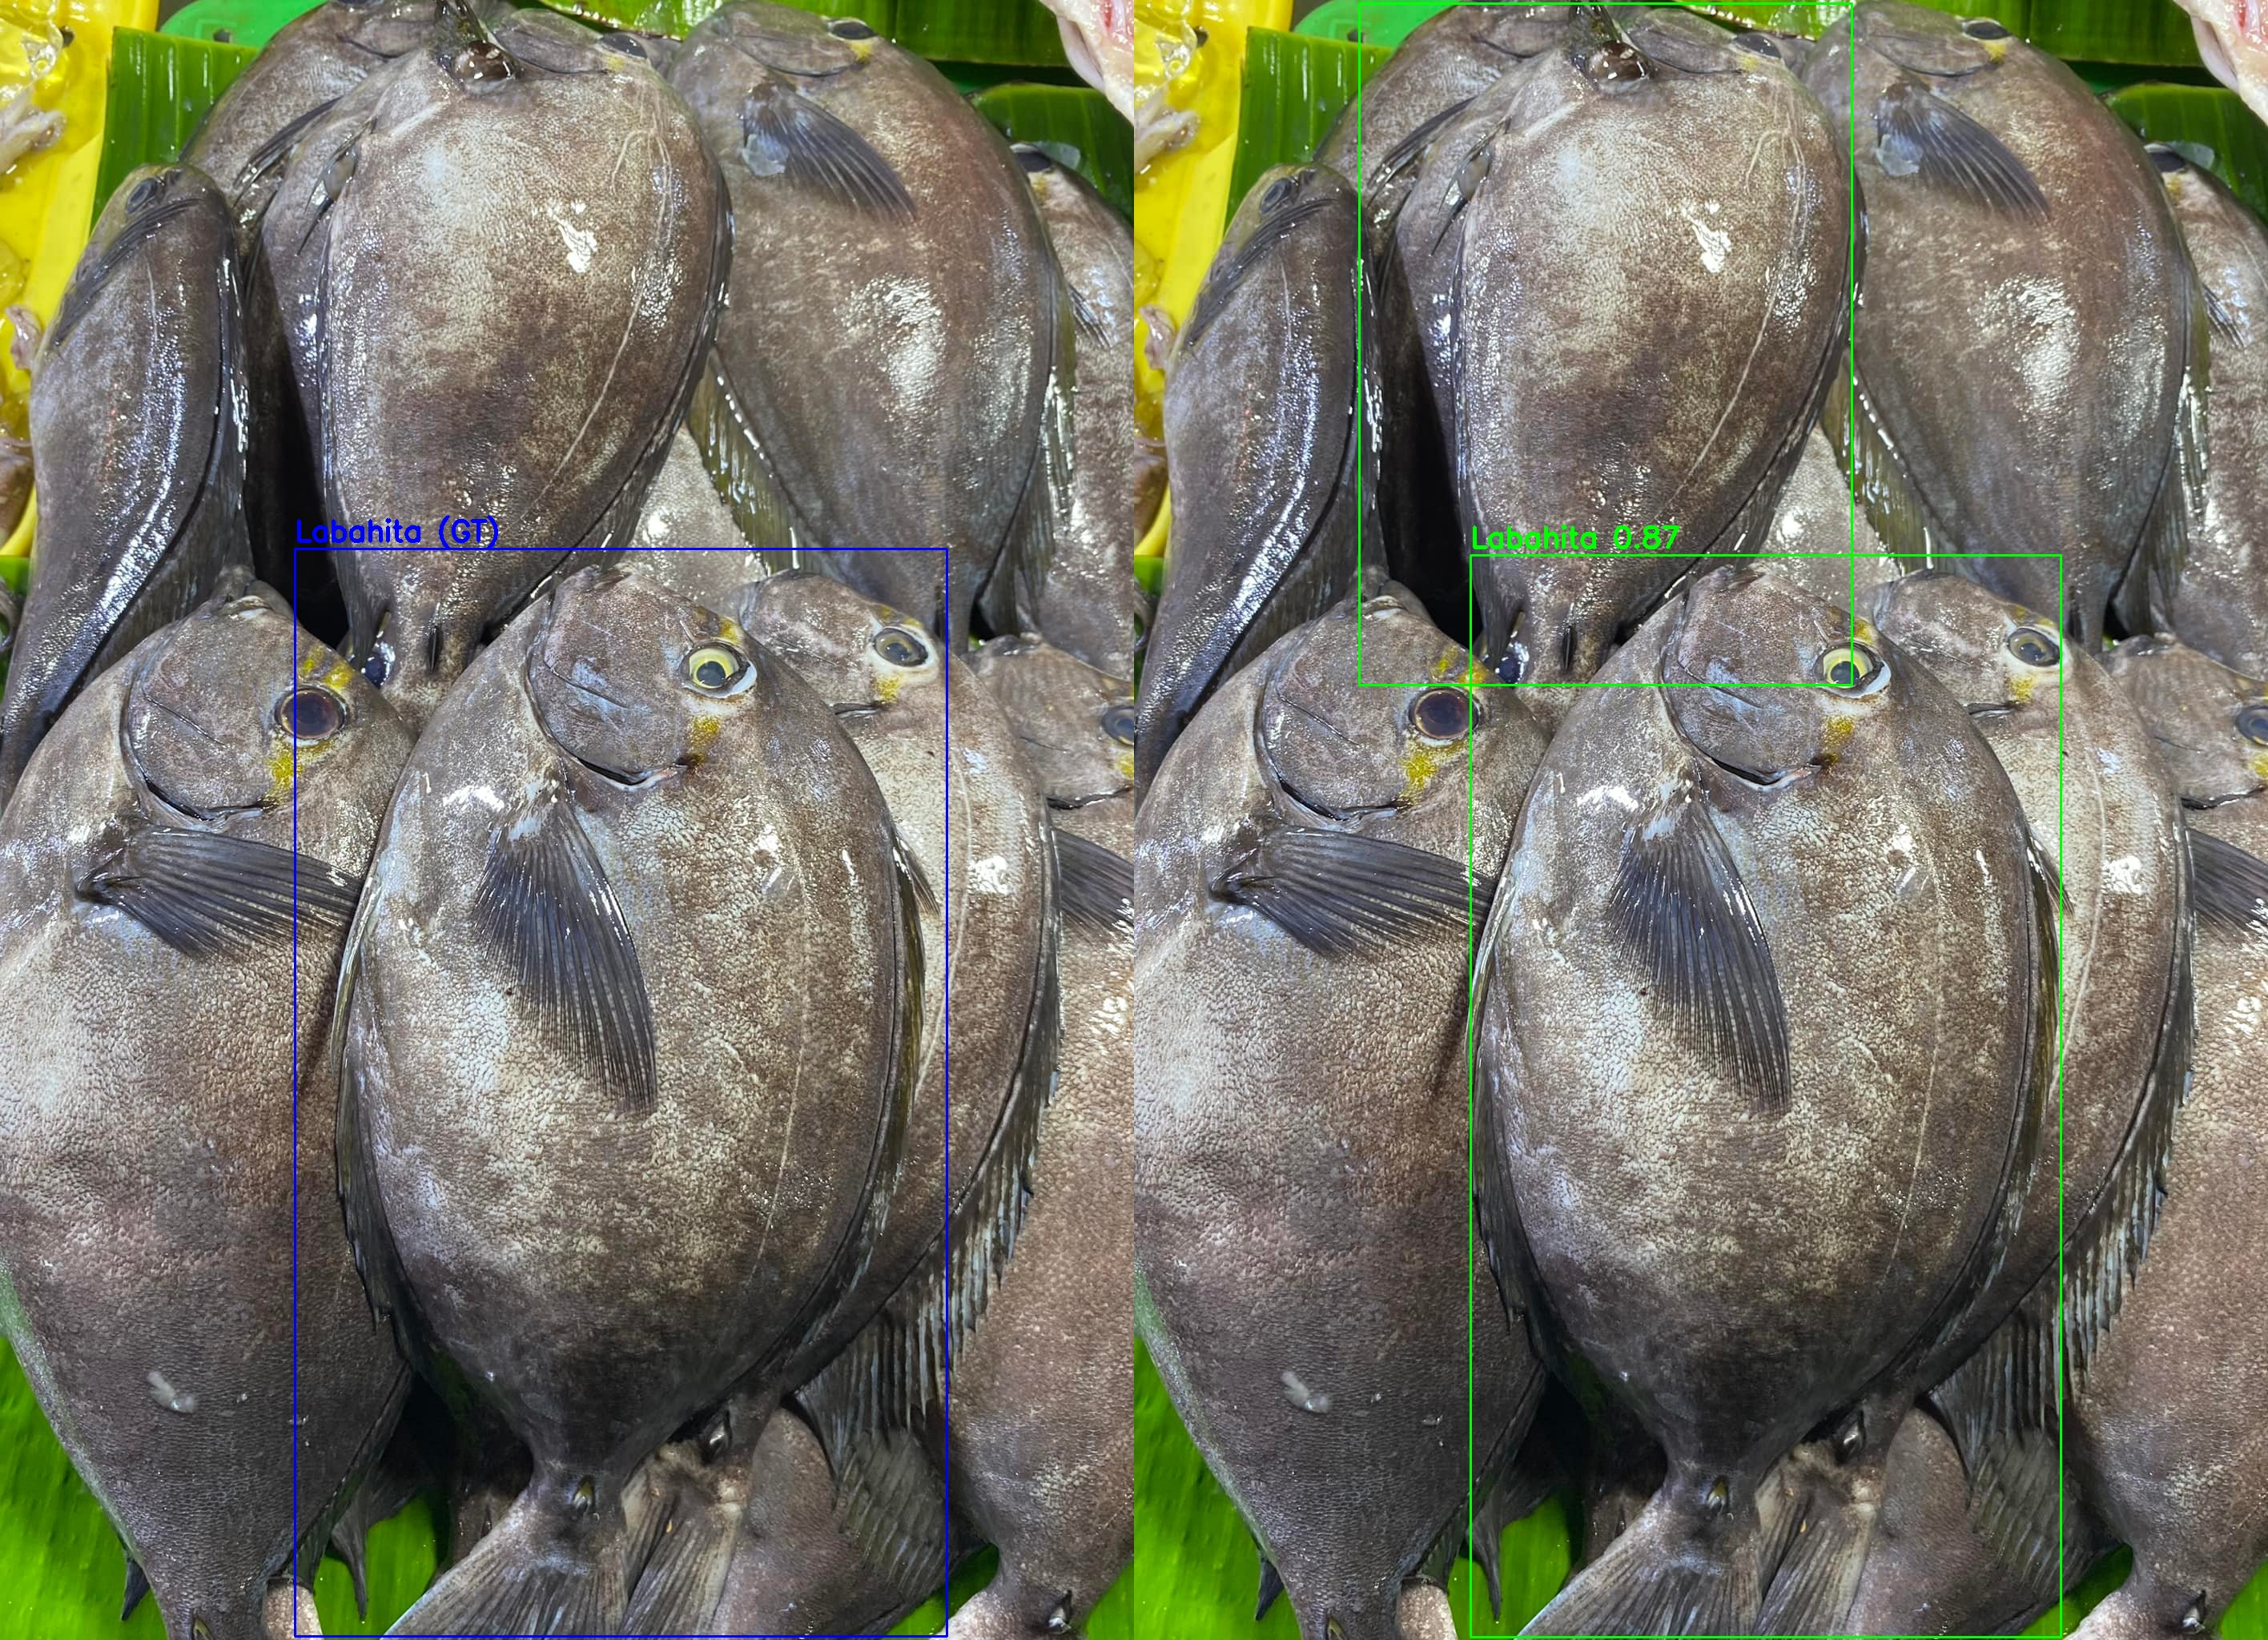
\includegraphics[width=0.8\textwidth]{images/images/predictions_per_class/Labeled_Labahita_Detected_Labahita.jpg}
    \caption{Ground Truth vs. Predicted Bounding Boxes for Labahita} 
    \label{fig:Labahita}
\end{figure} 





\newpage

\section{ClassiFish Mobile Development Using Agile SDLC Framework}
\subsection{Requirements Collection and Planning}
During this phase, the initial requirements were gathered to identify the key functionalities of the mobile application. These included the integration of the YOLOv11 model for fish detection, the presentation of ecological and nutritional information, and the implementation of a feedback mechanism to support continuous model retraining.

The key requirements included:

\begin{itemize}
    \item Capturing and processing images to enable the detection of fish species.

    \item  Display the predicted fish species along with ecological and nutritional details.
    
    \item Include a feedback mechanism for users to confirm or correct the identified species.

    \item Implementing backend support to receive and process feedback.

    \item Process for retraining and deploying updated models based on feedback.
\end{itemize}

These requirements were converted into a product backlog that guided sprint planning. Each sprint involved prioritizing items from the backlog, breaking them down into manageable tasks, and setting clear development goals such as configuring the development environment and designing the database schema.

\noindent\textbf{Core Functionality: Fish Detection}
\begin{itemize}
    \item Implement real-time fish detection using the device camera.
    \item Implement fish detection from gallery images.
    \item Integrate the trained YOLOv11 model (TensorFlow Lite) into the mobile application.
    \item Display bounding boxes and predicted species labels on detected fish.
\end{itemize}

\noindent\textbf{Fish Information Display}
\begin{itemize}
    \item Retrieve and display detailed information about the identified fish species (name, taxonomic classification, description, nutrition, conservation status, health benefits).
    \item Store fish species information locally on the device (SQLite) for offline access.
\end{itemize}

\noindent\textbf{User Feedback Mechanism}
\begin{itemize}
    \item Allow users to indicate whether a detection is correct or incorrect.
    \item If incorrect, allow users to select the correct fish species from a list.
    \item Capture and store feedback data (original image, user correction, timestamp, model prediction) locally.
\end{itemize}

\noindent\textbf{Backend System}
\begin{itemize}
    \item Develop RESTful API endpoints for mobile-backend communication (user authentication, feedback submission, fish info retrieval, model updates).
    \item Implement user authentication and management on the backend.
    \item Design and implement the centralized backend database schema (users, fish species, feedback, detection logs, ML model metadata).
    \item Implement logic for receiving and storing user feedback.
    \item Implement logic for retrieving fish species information.
\end{itemize}

\noindent\textbf{Web Admin Panel}
\begin{itemize}
    \item Implement admin user authentication (login, registration).
    \item Develop an interface for reviewing user-submitted feedback.
    \item Implement functionality for administrators to approve or reject feedback based on external references.
\end{itemize}


Using an Agile approach enabled flexibility while maintaining a clear study direction. Focusing on essential features in early sprints helped ensure critical components were addressed first. Ecological and nutritional information was sourced from reputable institutions, including government fisheries agencies and academic sources, ensuring reliable data for end-users.


\subsection{Analysis}
\begin{itemize}
\item \textbf{YOLOv11 Compatibility and Performance:}
The YOLOv11 model was converted to TensorFlow Lite and integrated into the mobile application. Compatibility with Android devices was observed, allowing real-time object detection to function within the constraints of mobile hardware. The model ran with minimal latency during testing, indicating suitable performance for mobile deployment.

\item \textbf{Key Features Implementation:}
The mobile application was developed to support key features for fish-based detection, including image capture through the camera or gallery, fish species identification, retrieval of species-related information, and user feedback submission.
\end{itemize}

\subsection{Designing}
The designing phase produced the blueprints for the application's architecture, and data flow.

\subsubsection{Database Schema Design:} Using SQLite, a database schema was designed to store fish species information, user feedback, and detection history.

The database schema included tables for fish species information such as name, description, and ecological information. For feedback entries, there were several tables containing image reference, predicted species, corrected species, and timestamp. For detection logs; the tables included image reference, predicted species and timestamp.
\begin{figure}[H]
    \centering
    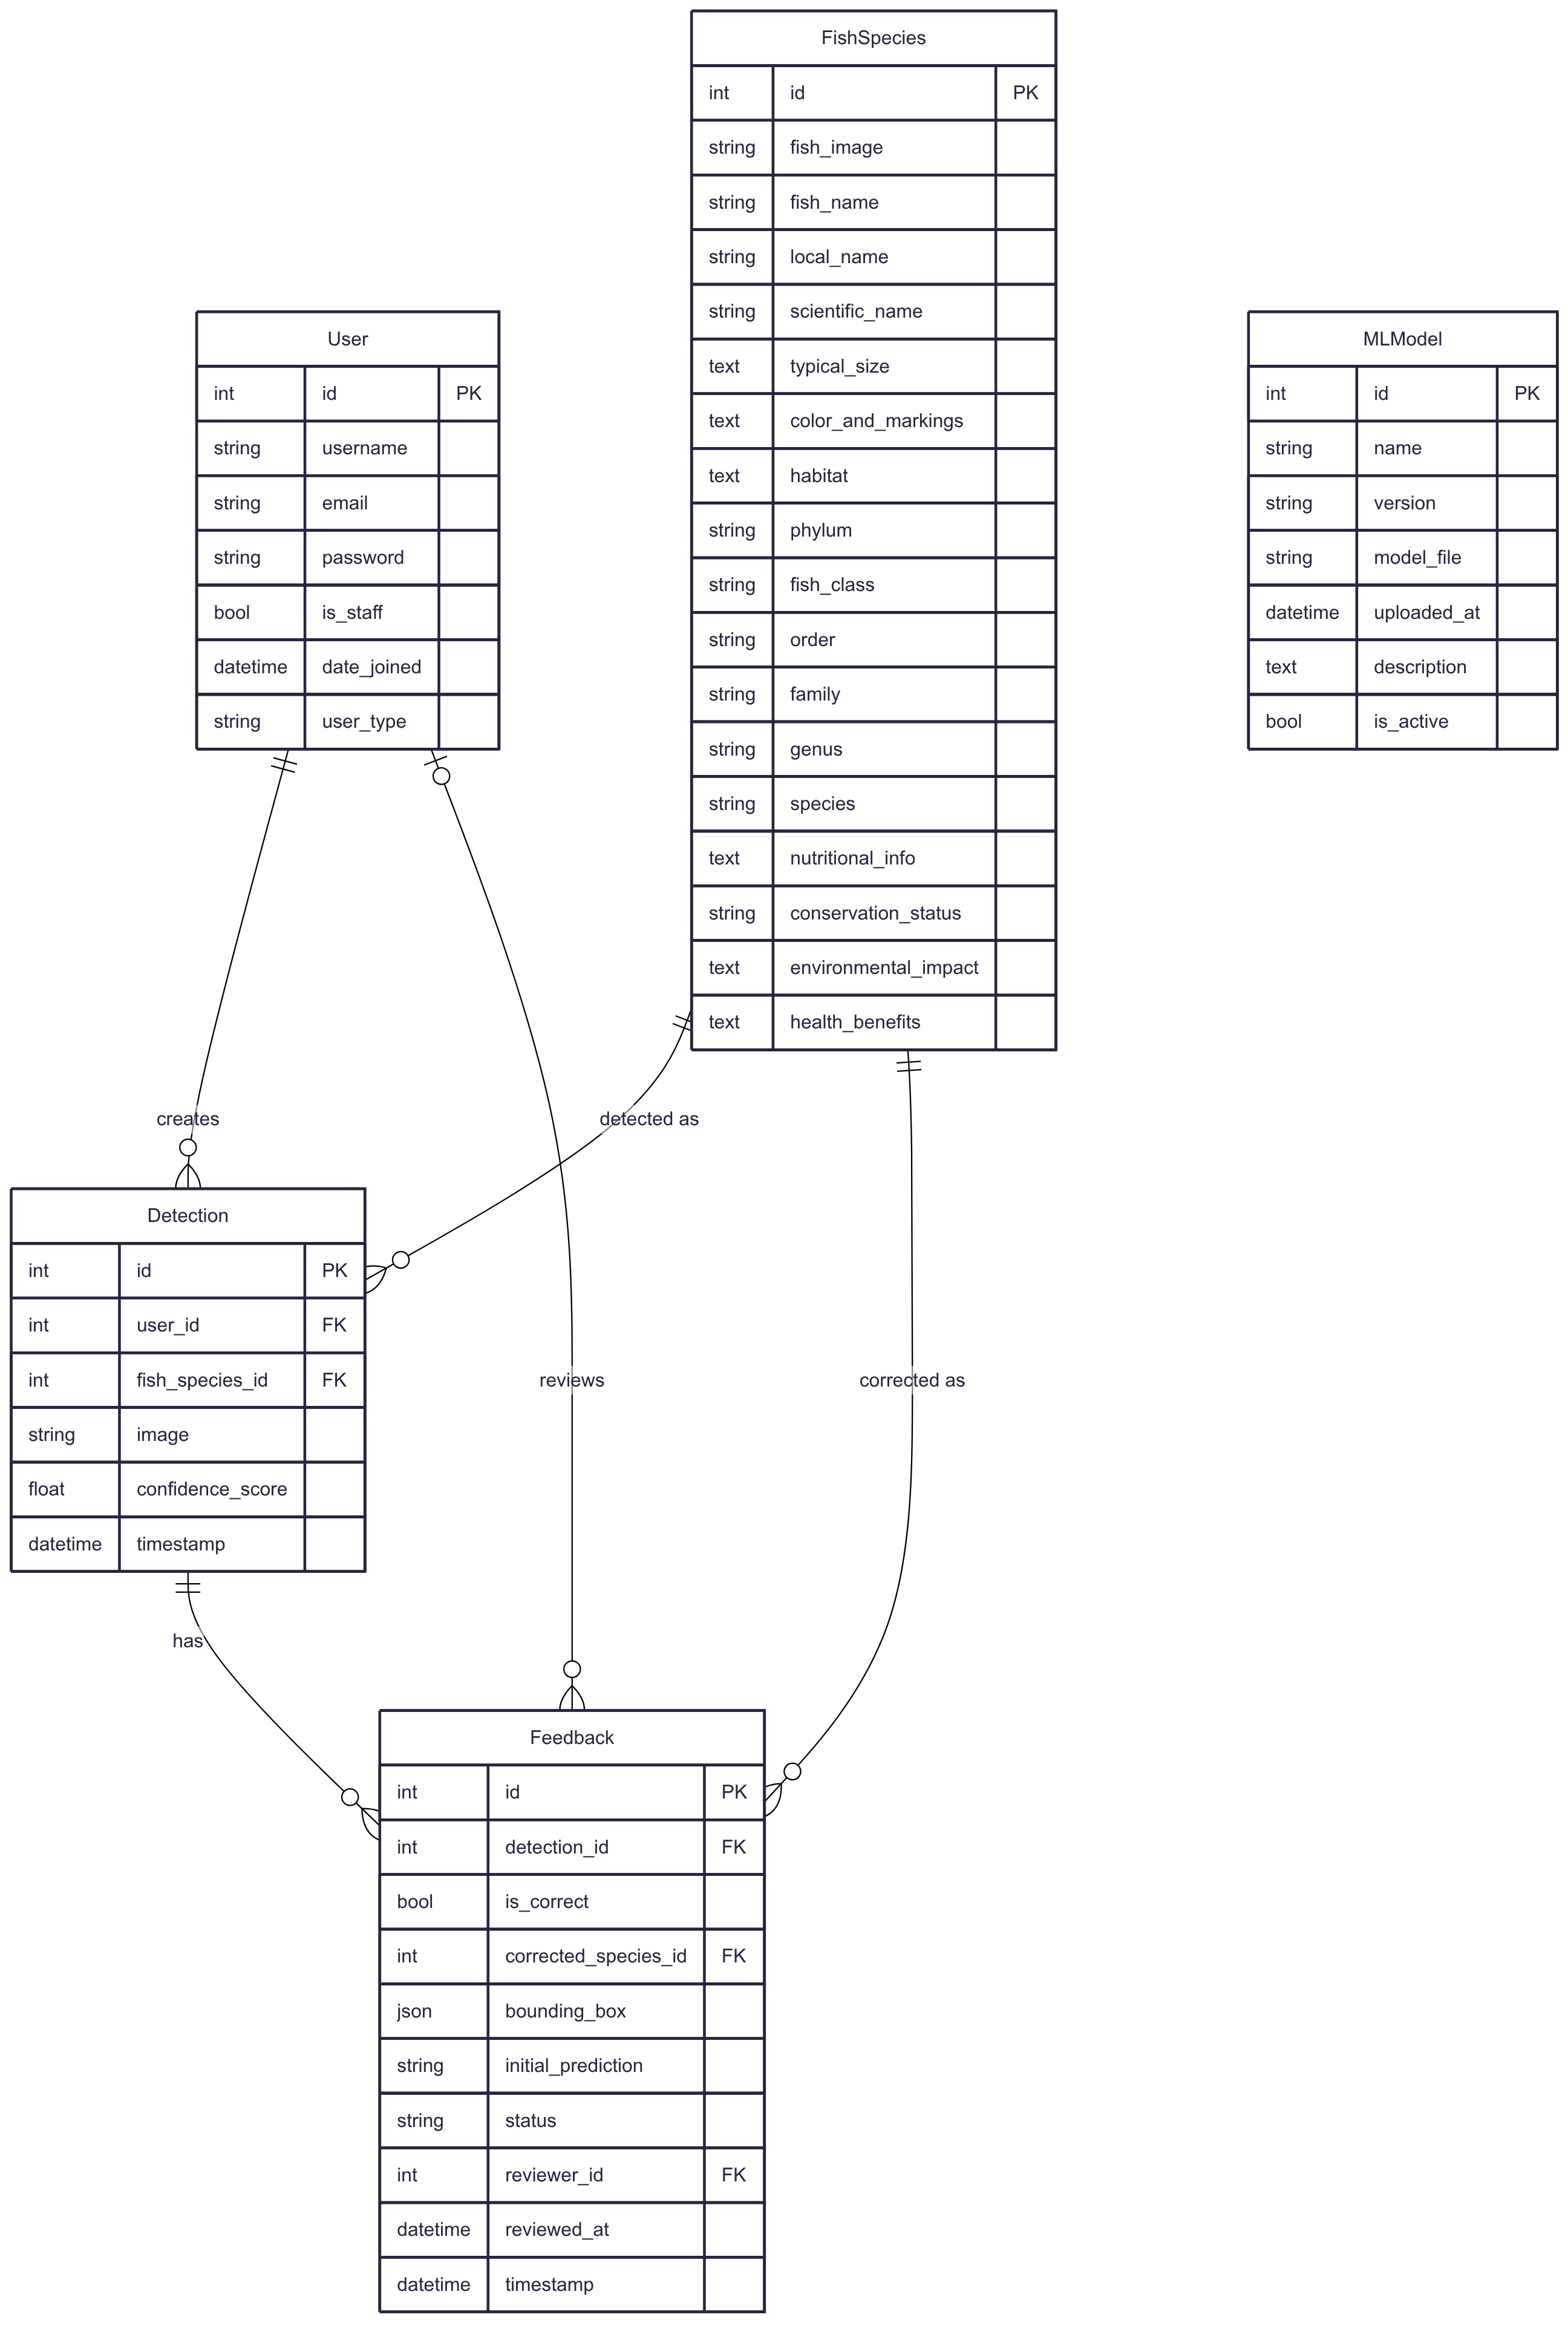
\includegraphics[height=0.85\textheight]{images/images/mobile_app/revision/ERDupdated.png}
    \caption{Entity Relationship Model}
\end{figure}

\subsubsection{UI/UX Design:} Mockups and prototypes were created in Figma to design the mobile application's user interface. The design prioritized ease of use, with clear navigation for image capture, viewing detection results, accessing fish information, and submitting feedback.

\subsubsection{API Design:} RESTful API endpoints were designed to facilitate communication between the mobile application and the Django backend. These endpoints handled user authentication, feedback submission, retrieval of fish species information, and potentially for downloading updated models.

\begin{figure}[H]
    \makebox[\textwidth][c]{%
        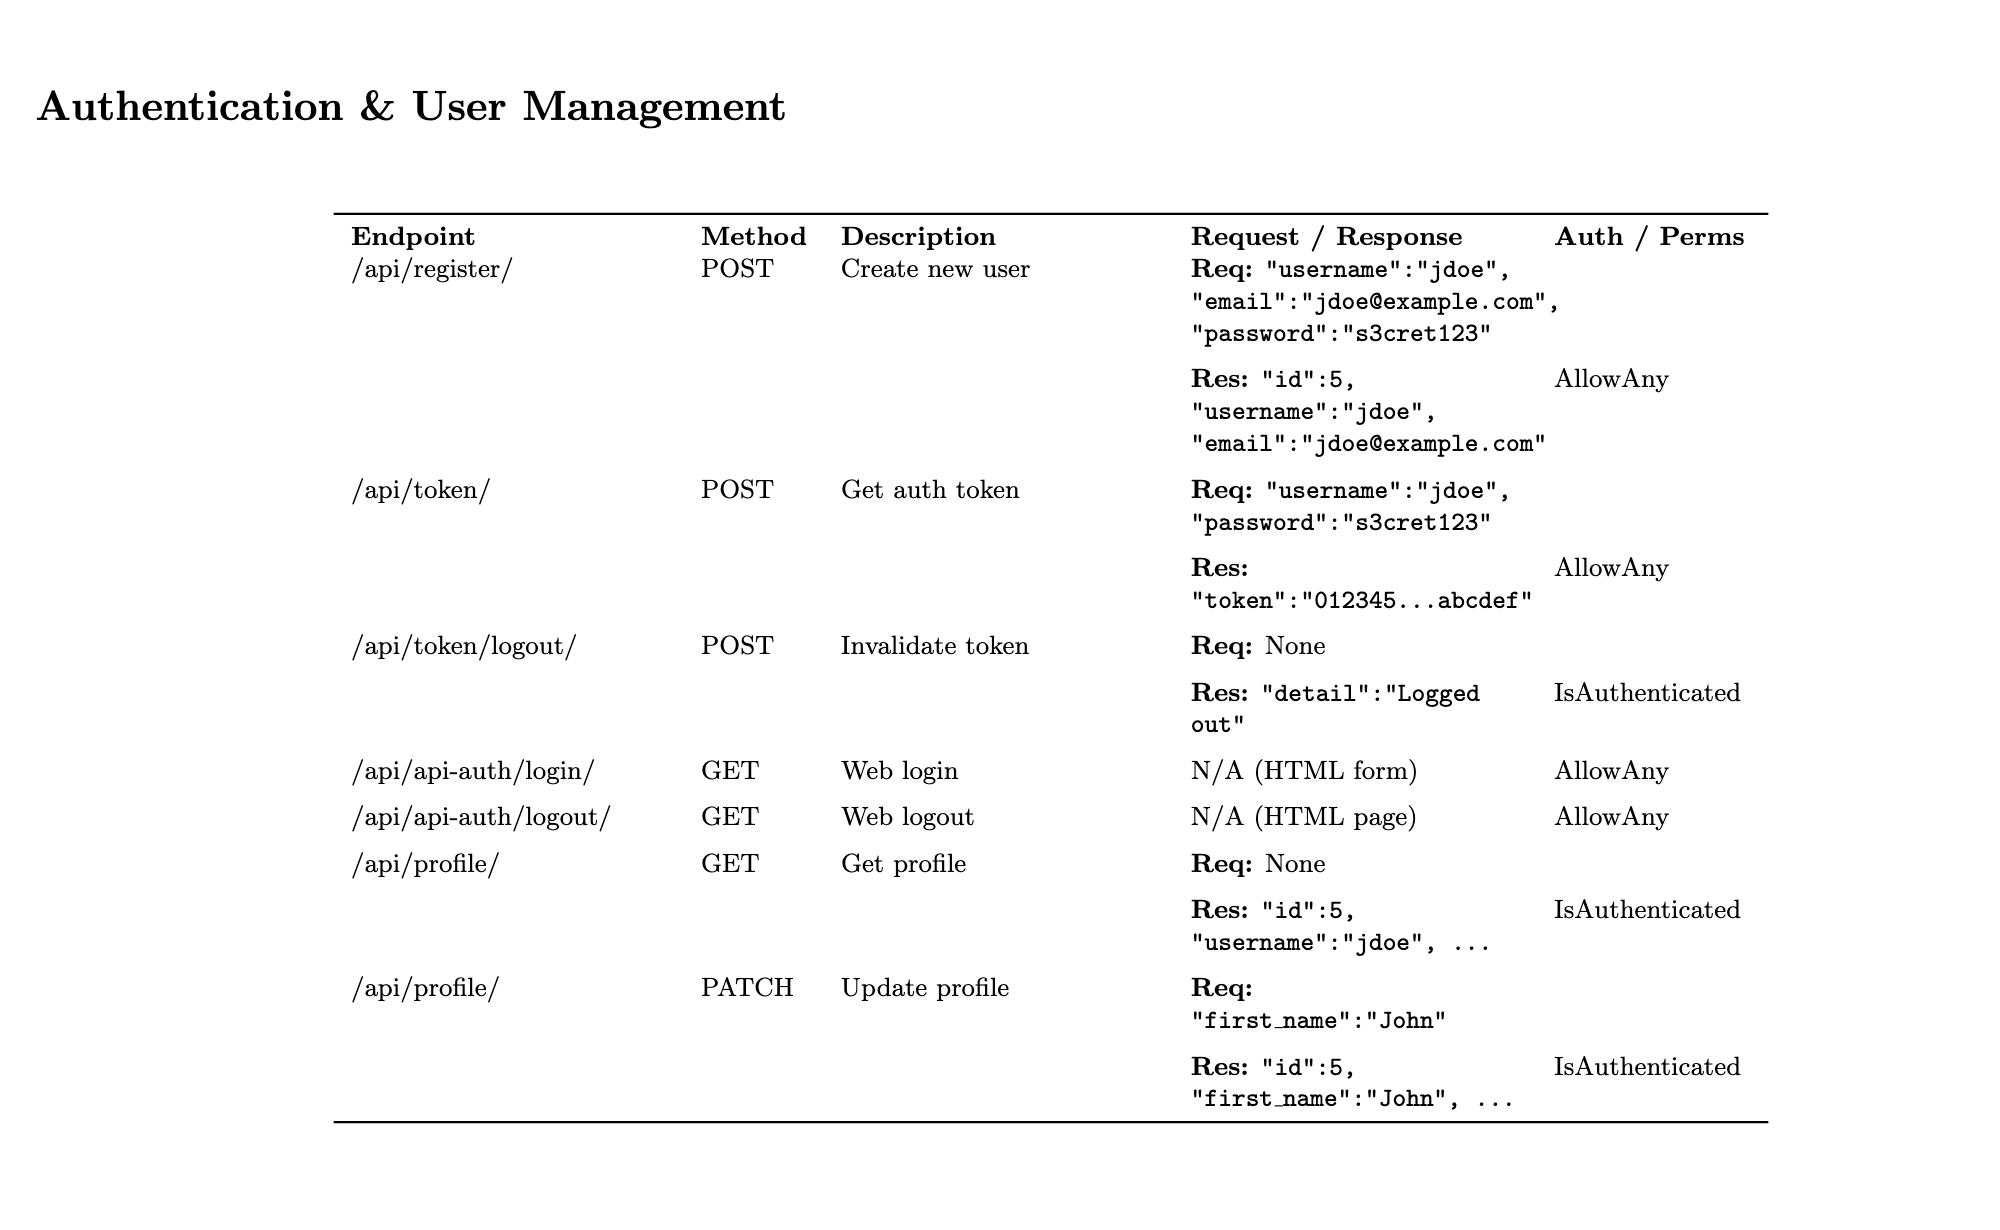
\includegraphics[width=1.2\textwidth]{images/images/SDLC/API1.png}%
    }
    \caption{Authentication and Management API}
\end{figure}

\begin{figure}[H]
    \makebox[\textwidth][c]{%
        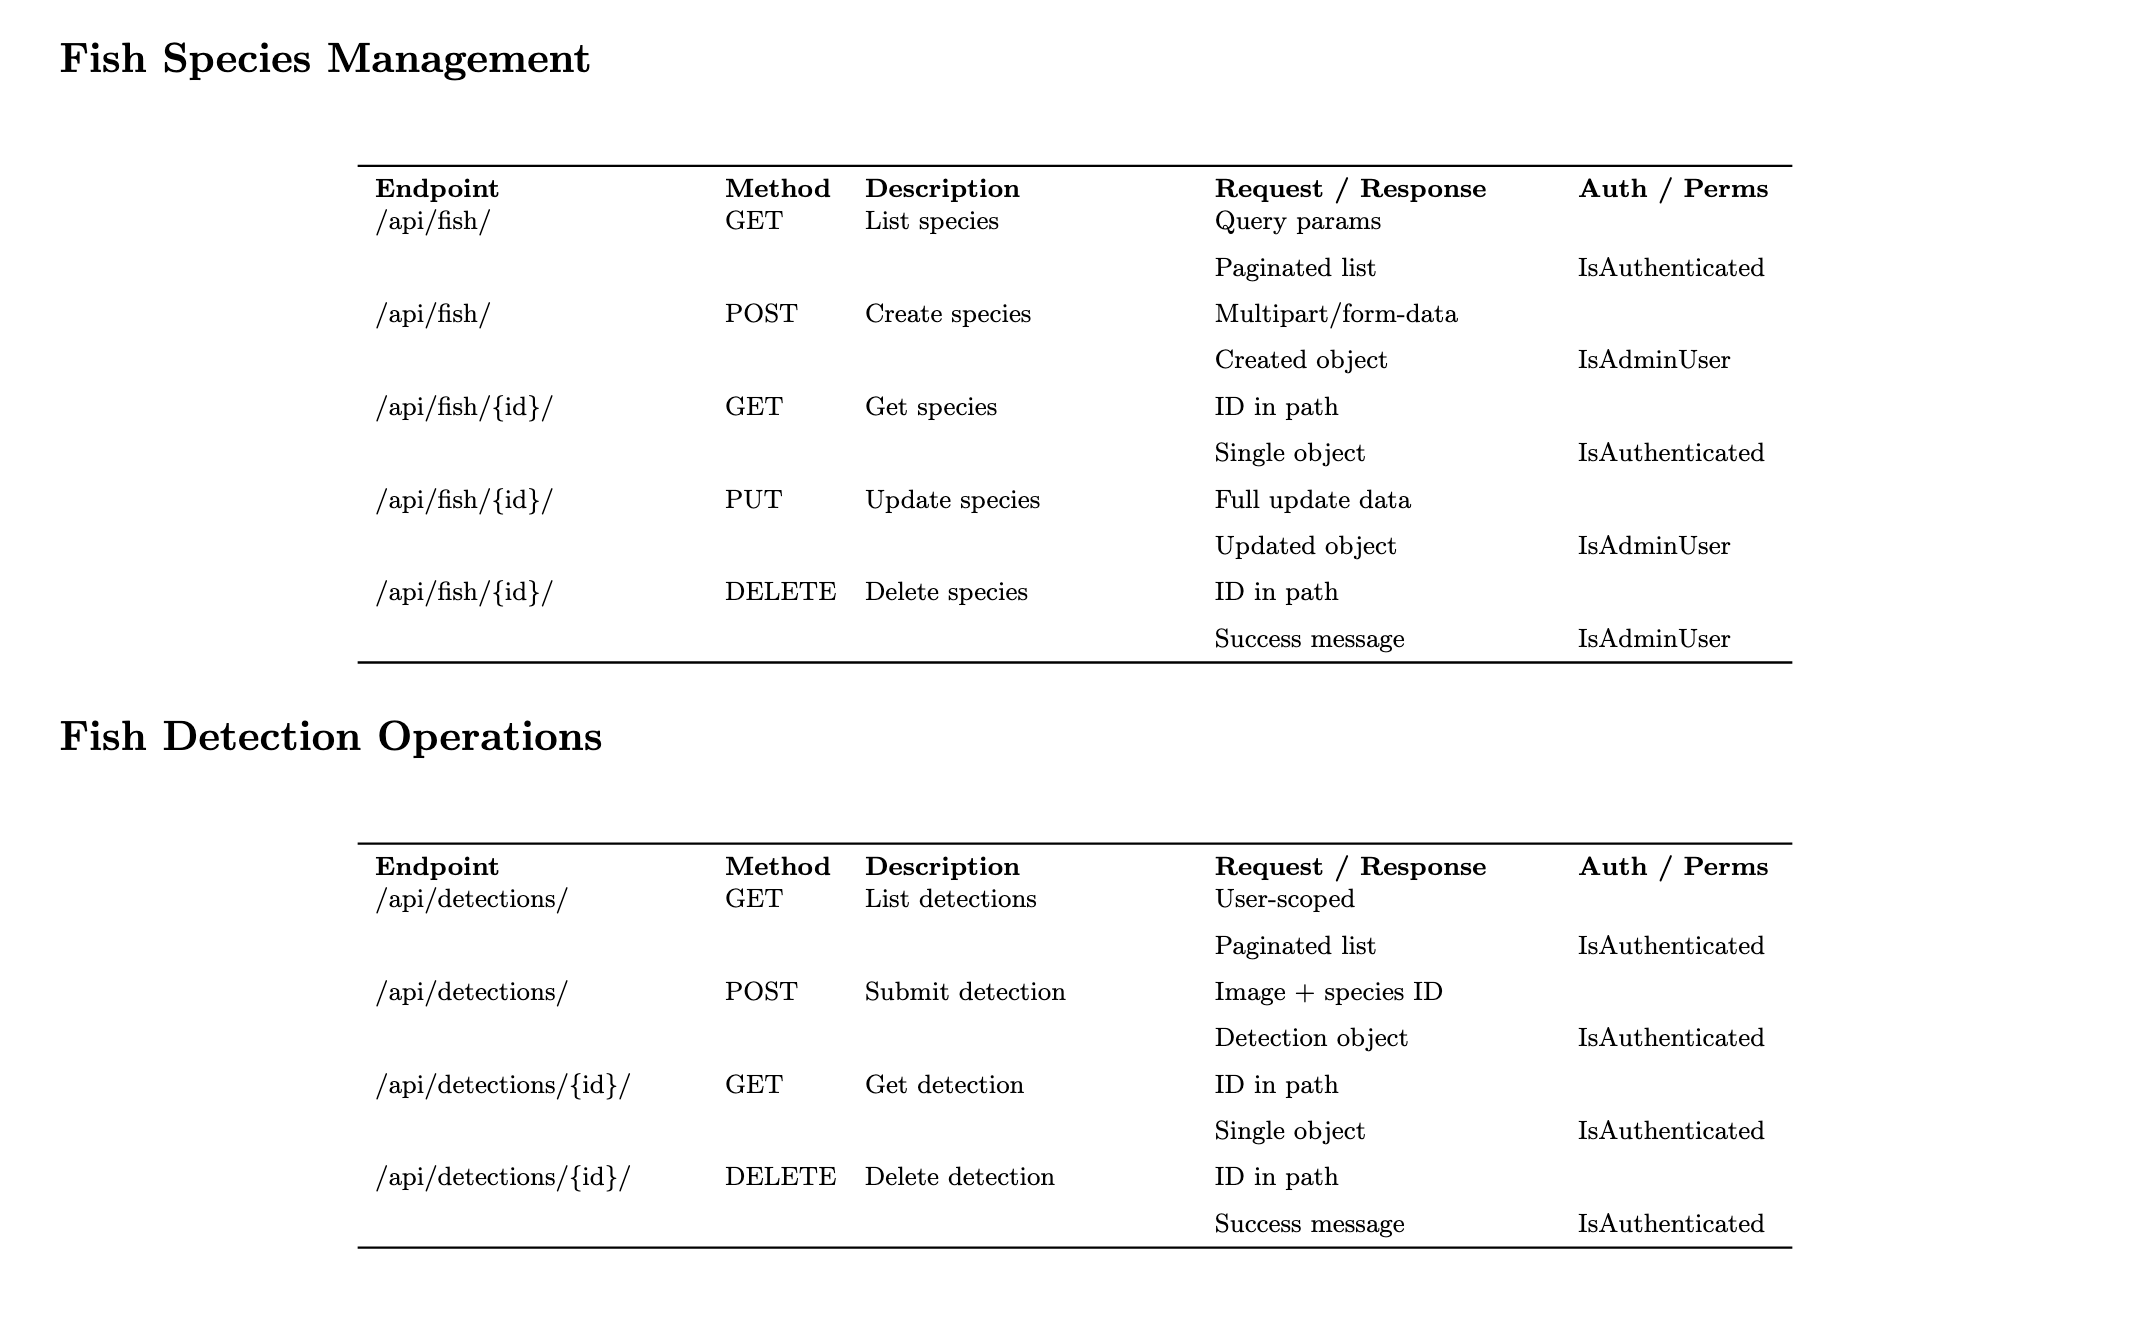
\includegraphics[width=1.15\textwidth]{images/images/SDLC/API3.png}%
    }
    \caption{Fish Species and Fish Detection API}
\end{figure}

\begin{figure}[H]
    \makebox[\textwidth][c]{%
        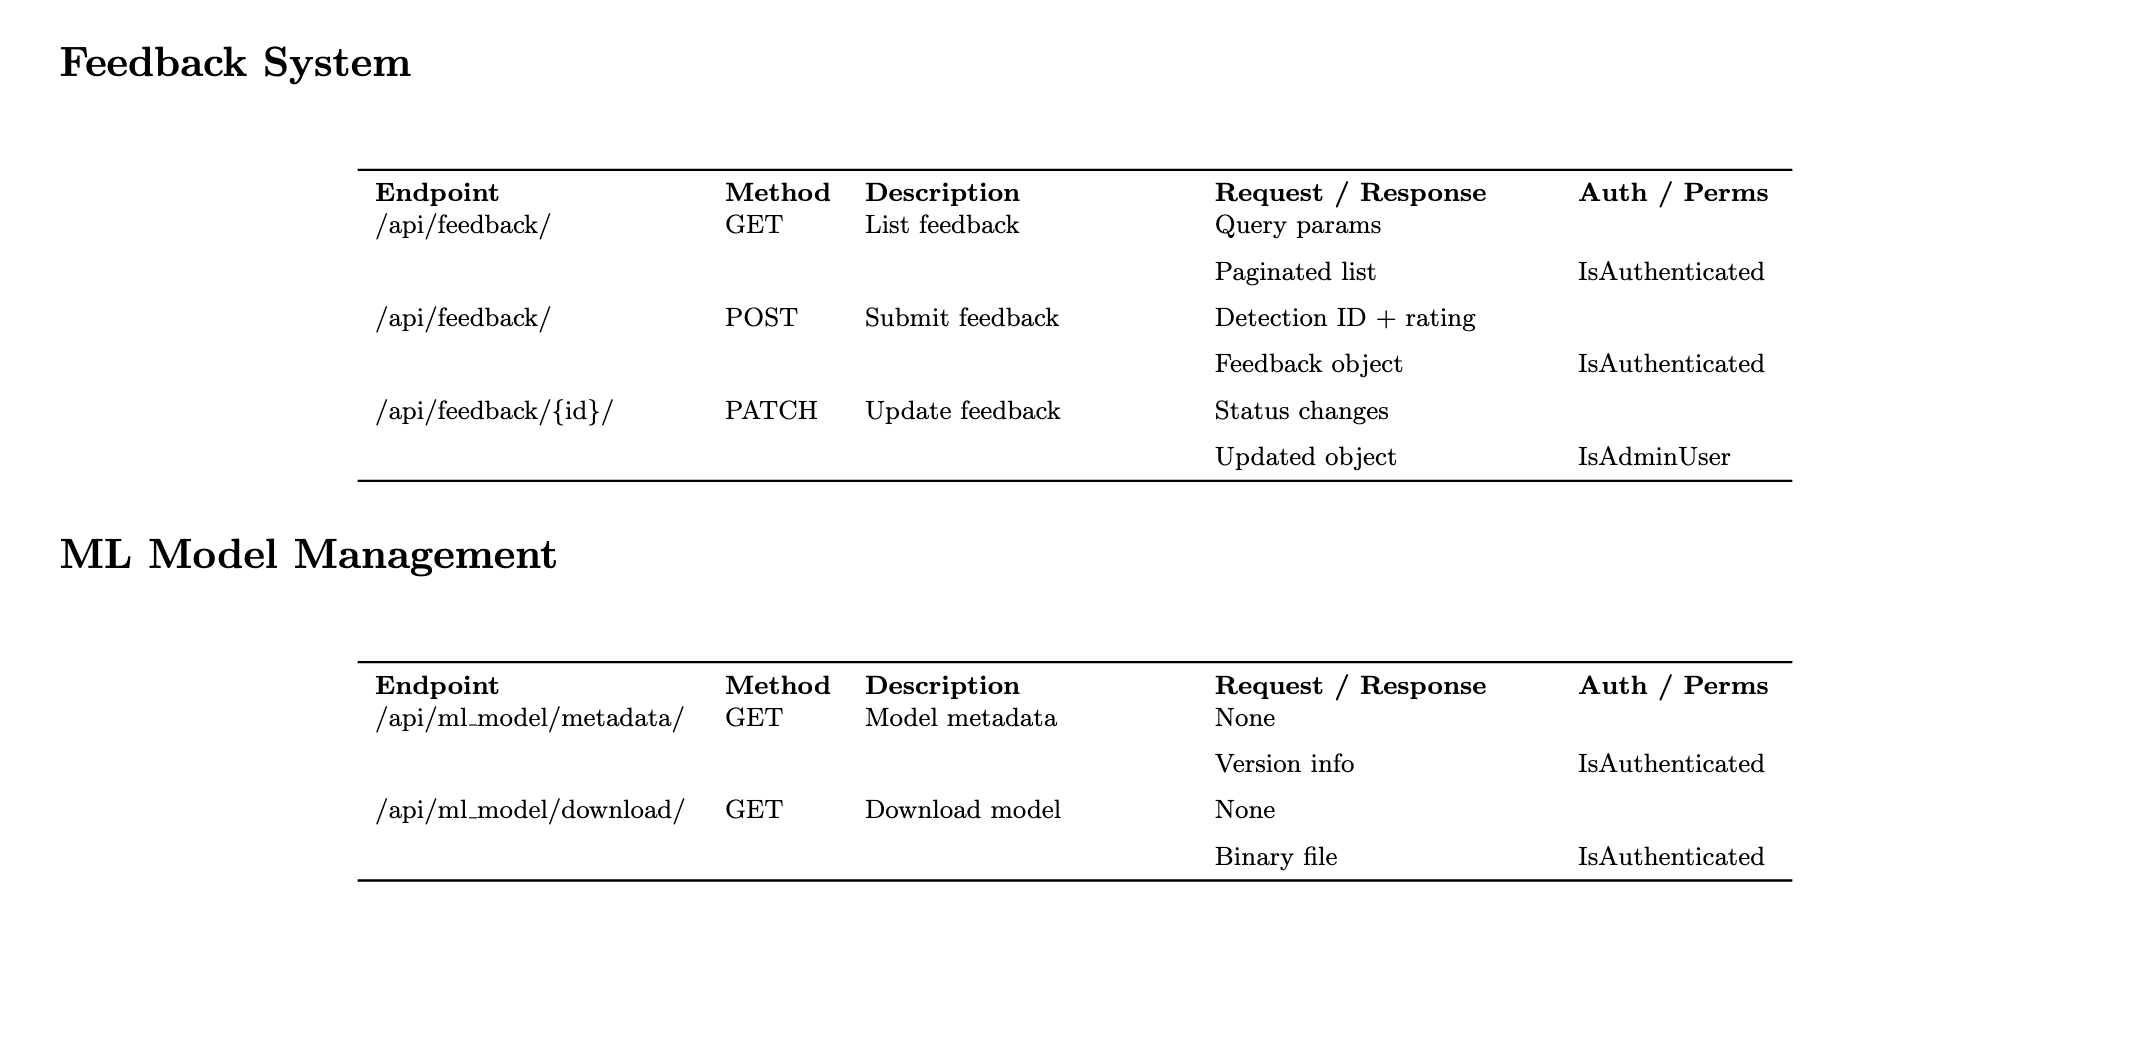
\includegraphics[width=1.15\textwidth]{images/images/SDLC/API4.png}%
    }
    \caption{Feedback System and ML Model Management API}
\end{figure}

The design phase laid a strong foundation for the following development phase. SQLite was selected as a database for its suitability for mobile applications, allowing local data storage and offline access functionality. The UI/UX design prioritized ease of use to enhance user experience to encourage engagement and feedback submission.  Additionally, the RESTful API was designed to provide a standardized and efficient communication channel between the mobile application and backend, supporting both data synchronization and future scalability.

\subsection{Coding}
The coding phase involved the implementation of the mobile application using Flutter and the backend server using Django.

\begin{itemize}
    \item\textbf{Mobile App Development:} The Flutter application was developed,incorporating the key features including image capture using the camera plugin, UI components designed based on the Figma mockups, and local data storage using SQLite through Drift package. Functional screens were implemented for fish detection, results display, fish information, and feedback submission.

    \item\textbf{Server-Side Development:}The Django backend was developed, incorporating the REST API endpoints designed in the previous phase. Models for \texttt{FishSpecies}, \texttt{Feedback}, and \texttt{MLModel} were implemented, along with serializers and views to manage API requests. Additionally, an admin panel was set up to facilitate feedback review.

    \item\textbf{Database Implementation:} The SQLite database schema was implemented within the Flutter application using Drift, and the Django backend interacted with its database models.

    \item\textbf{Model Integration:} The trained YOLOv11 model, converted into TensorFlow Lite format, was successfully integrated into the Flutter application using the \texttt{ultralytics\_yolo} package. The app was able to load the model and perform inference on captured images.
\end{itemize}


The Flutter enabled the cross-platform development, reducing development time compared to building separate native application. Django provided a backend framework for fast API and database management, The integration of TensorFlow Lite allows on-device inference, reducing latency and internet dependency. 


\subsection{Testing}
The testing phase involved unit and integration testing to ensure the functionality of individual components and ensure they work together.

\begin{itemize}
    \item\textbf{Unit Testing:} The individual functions and components of both Flutter application and the Django backend were tested using unit tests. This included testing the camera functionality, model loading and inference, database operations and API endpoint responses.
    
    \item\textbf{Integration Testing:} These tests were performed to ensure proper communication and data exchange between mobile application, the SQLite database on the device, and the Django backend via the REST API. This also included the testing feedback submission and data synchronization processes.
\end{itemize}

Testing both the unit and integration levels was crucial for identifying and fixing bugs early in the development cycle. The unit tests were useful for identifying issues within the specific components, while integration tests ensured that the different parts of the system worked together seamlessly. The integration of test files in the project structure indicates that testing was considered during development.

\newpage
\subsection{Feedback Mechanism}
The maintenance phase incorporated a robust feedback mechanism and a process for continuous model retraining and deployment.


\begin{figure}[H]
    \makebox[\textwidth][c]{%
        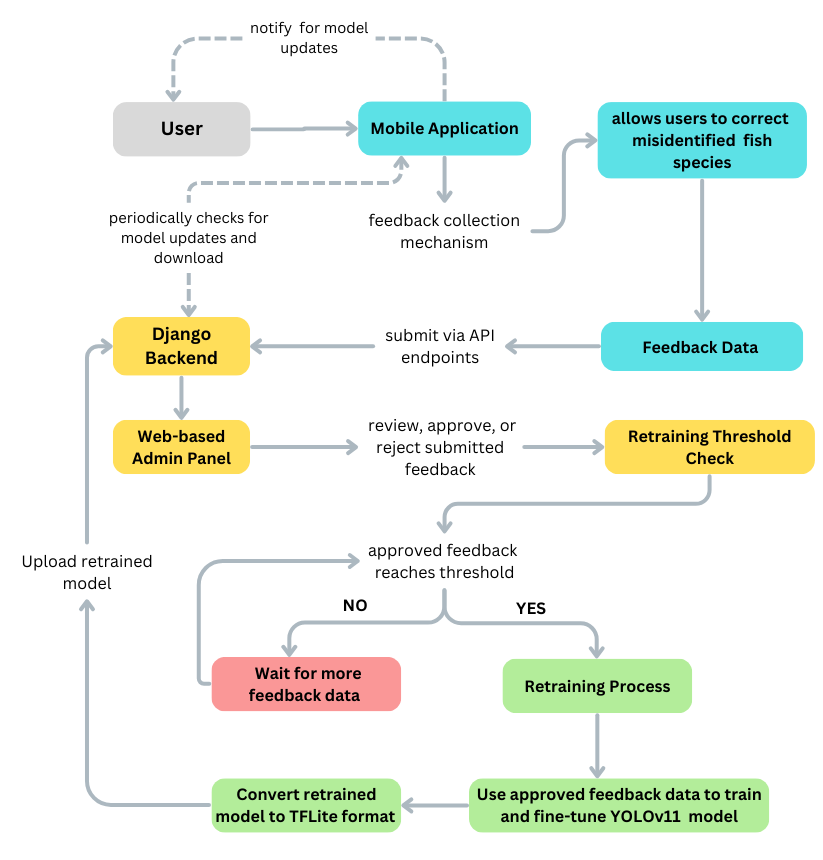
\includegraphics[width=1.1\textwidth]{images/images/Feedback Mechanism Diagram.png}%
    }
    \caption{Feedback Mechanism Diagram}
\end{figure}


\begin{itemize}
    \item\textbf{Feedback Collection:} The mobile app successfully implemented the feedback collection mechanism, allowing users to correct misidentified fish species and submit associated images and metadata to the backend.
    
    \item\textbf{Data Synchronization:} The feedback data was successfully synchronized from the mobile device to the Django backend via the designed API endpoints. The batch upload mechanism helped manage server load.
    
    \item\textbf{Admin Review:} The web-based admin panel in the Django backend provided a functional interface for system administrators to review, approve, or reject submitted feedback.

    \item \textbf{Retraining Threshold and Process:} A uniform retraining threshold was applied across all fish species. Retraining was only conducted once all species accumulated the required number of validated incorrect feedback entries. The approved feedback data, combined with the original dataset, was then used to fine-tune the YOLOv11 model through a manual retraining process.

    \item \textbf{Model Deployment:} After retraining and evaluation, the updated TensorFlow Lite model was deployed through a new system release. The mobile application was updated accordingly, allowing users to benefit from the improved model in subsequent app versions.

\end{itemize}

The implemented feedback loop is a critical component for the long-term accuracy and relevance of the fish identification model. By allowing users to correct errors, the system can continuously learn and improve. The data synchronization and admin review processes ensure that the feedback is managed effectively and that only validated data is used for retraining. The automated retraining and deployment process ensures that model improvements are regularly delivered to the end-users, enhancing the application's value over time.

\pagebreak

\section{ClassiFish Mobile Application}

\begin{figure}[H]
    \centering
    % First row
    \begin{minipage}[b]{0.48\textwidth}
        \centering
        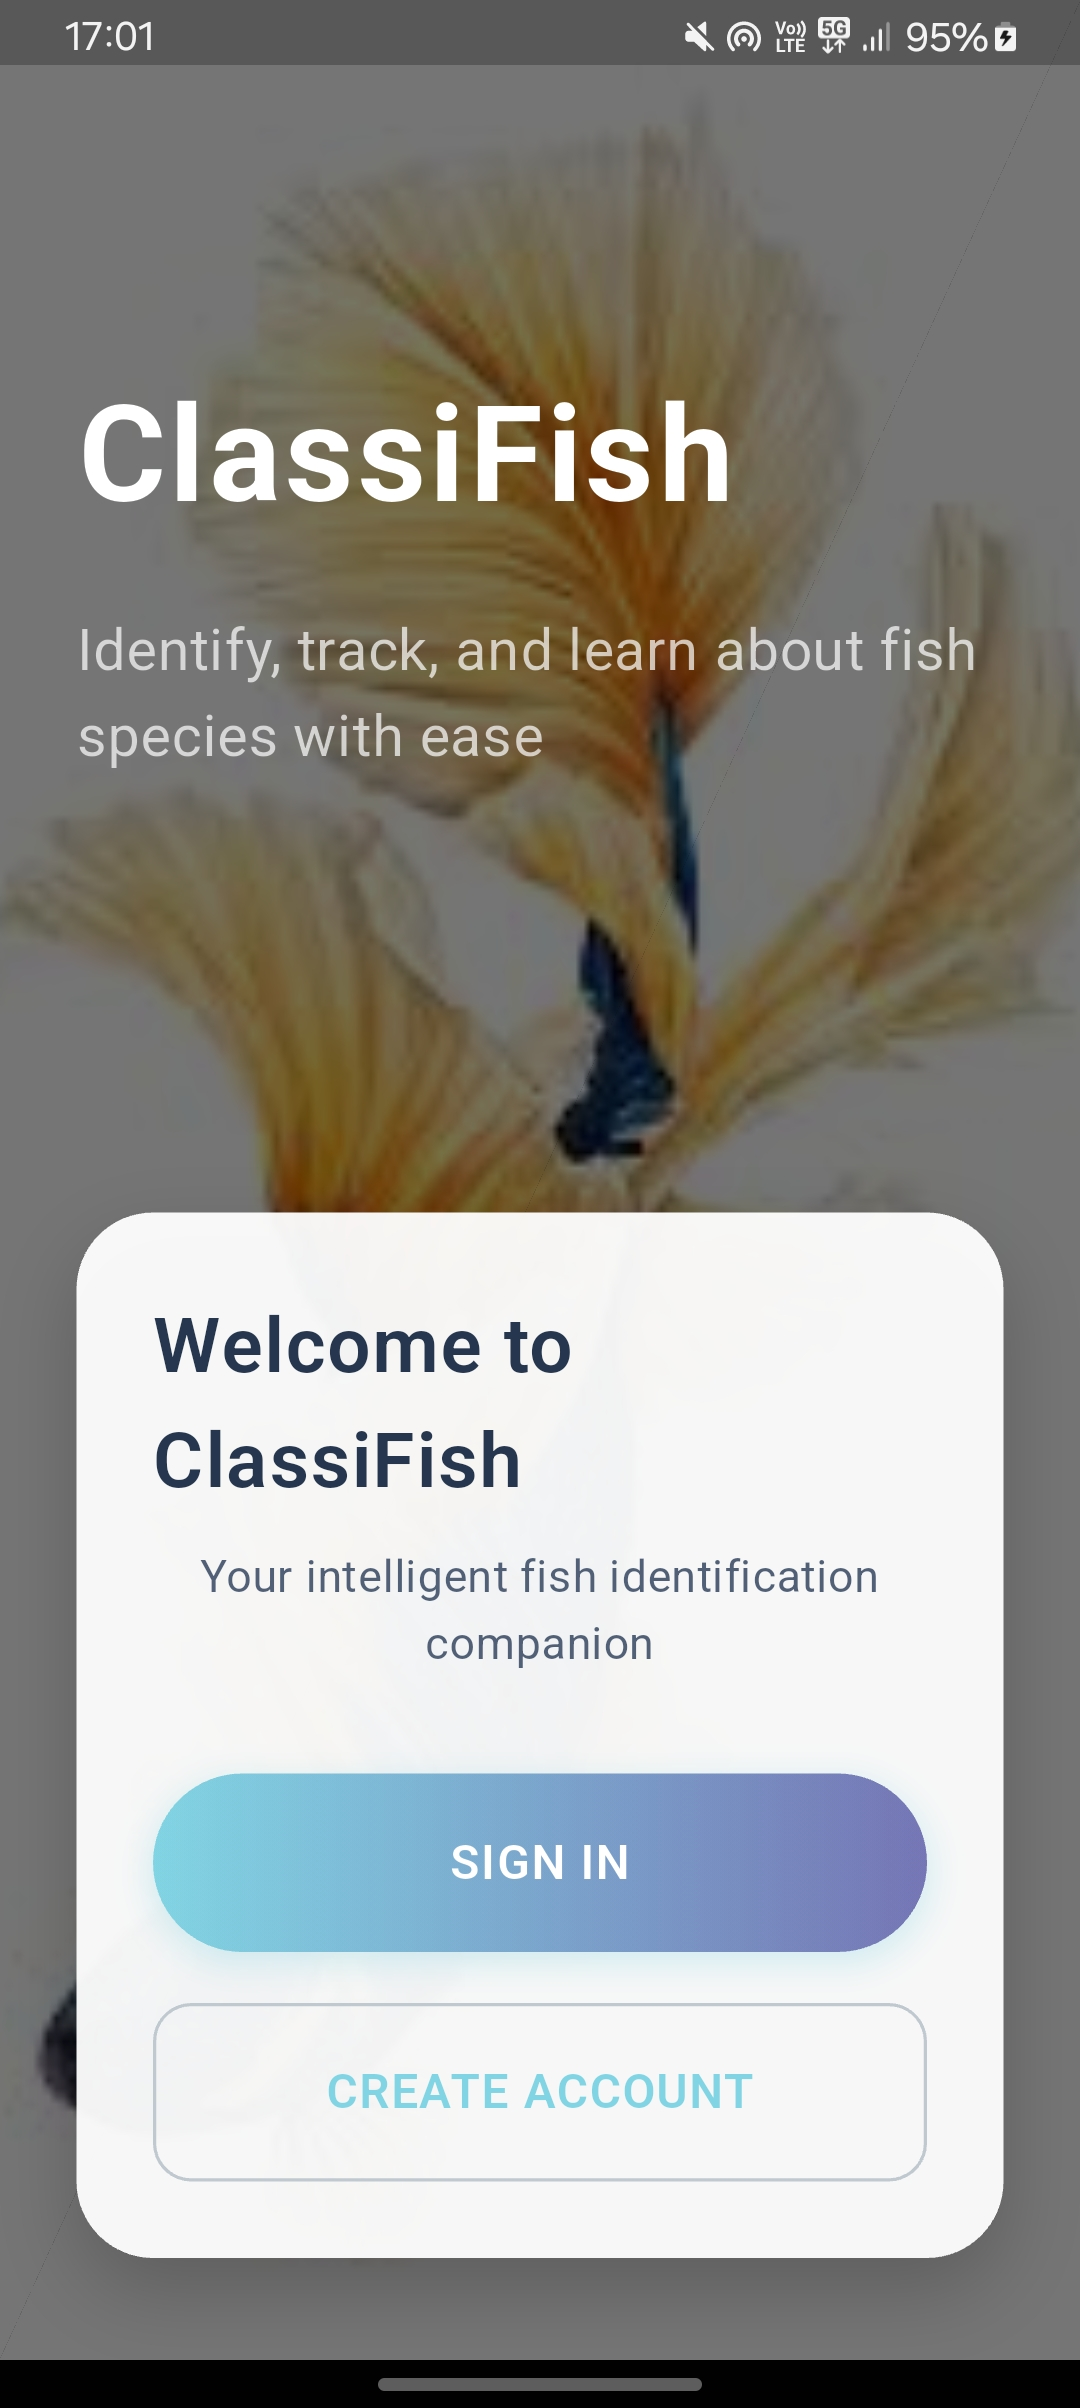
\includegraphics[height=0.5\textheight]{images/images/mobile_app/landing page.jpg}
        \caption{Landing Page}
    \end{minipage}
    \hfill
    \begin{minipage}[b]{0.48\textwidth}
        \centering
        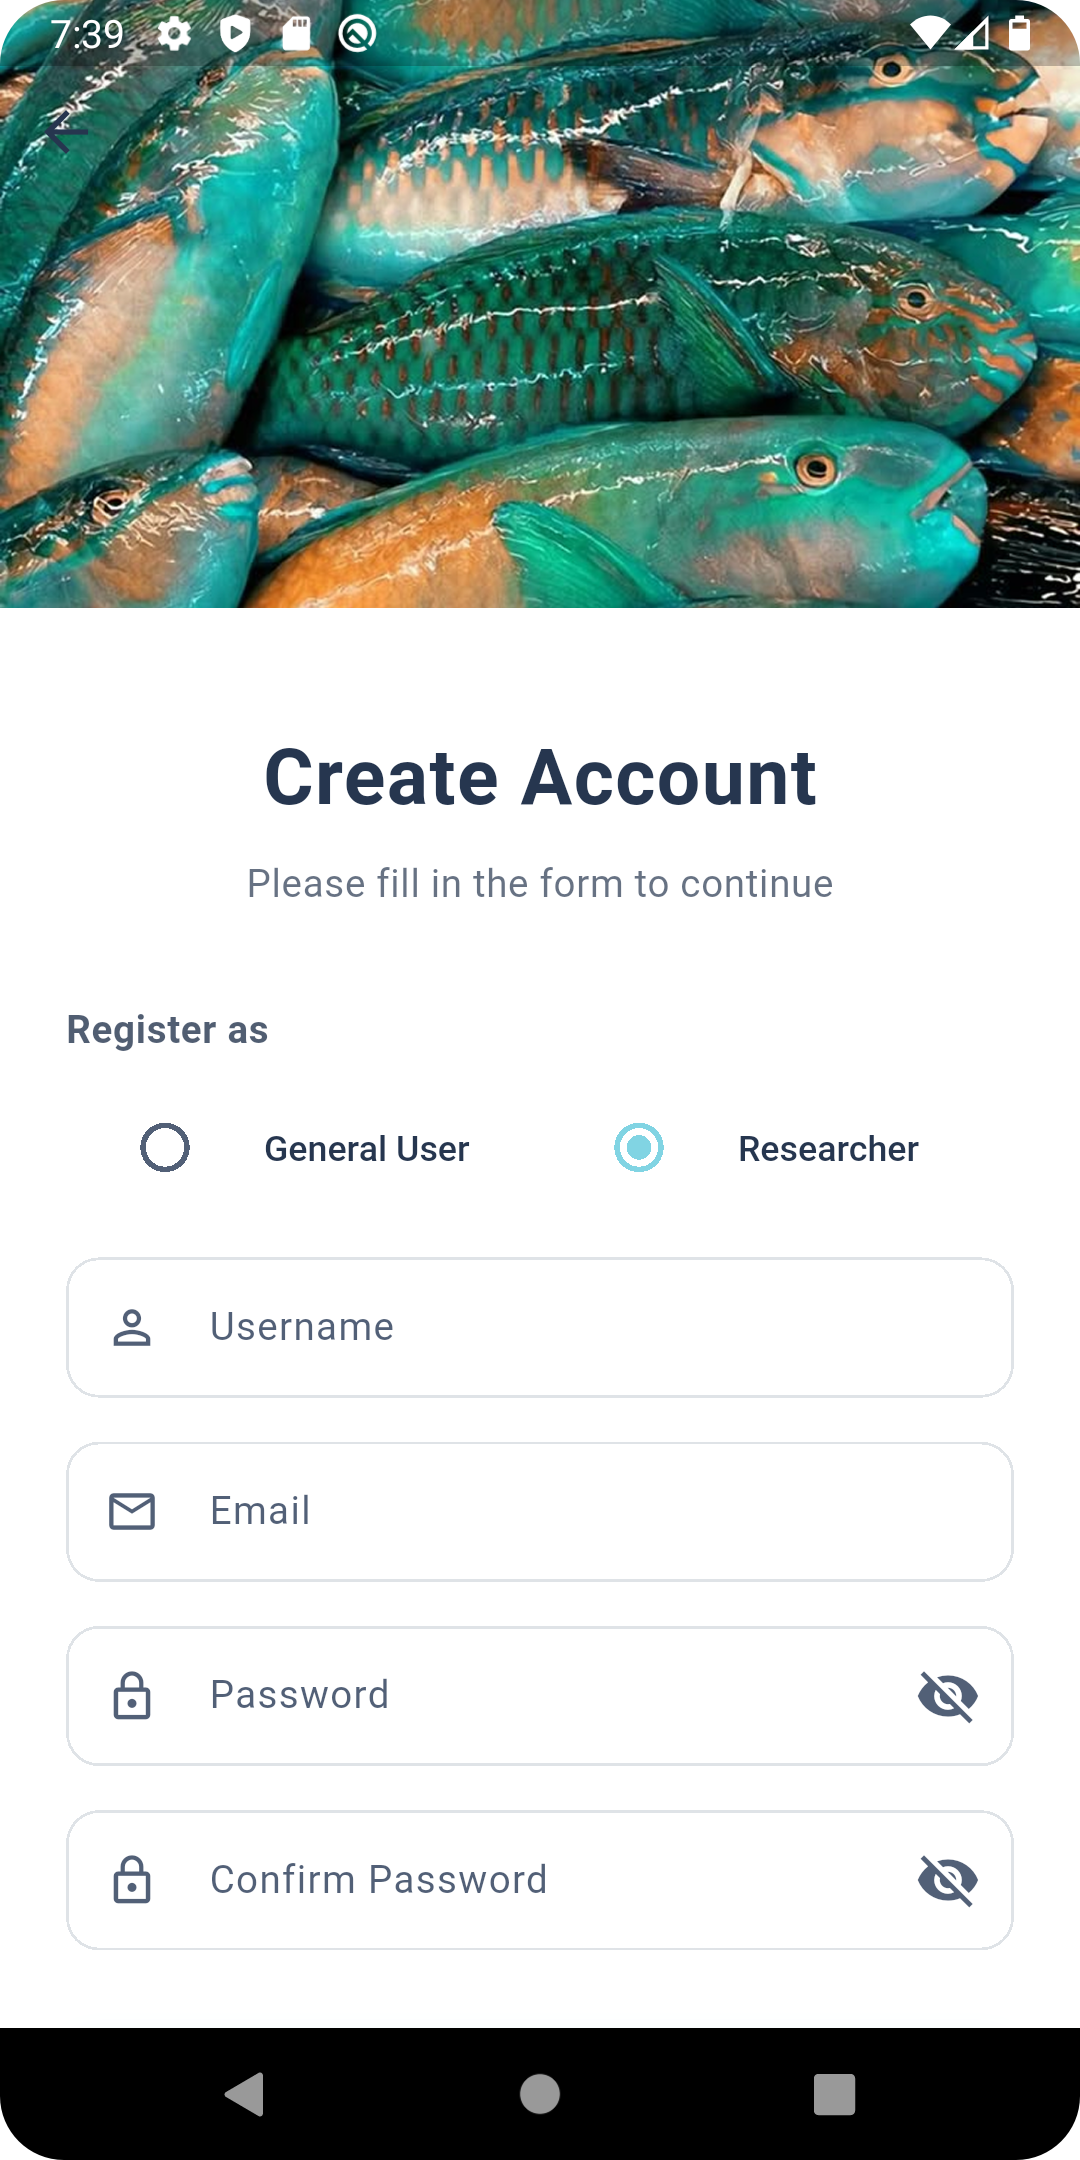
\includegraphics[height=0.5\textheight]{images/images/mobile_app/revision/SelectUserType.png}
        \caption{Sign Up}
    \end{minipage}
\end{figure}


\subsection{User Authentication}
The mobile application includes two main screens for user authentication: the Landing Page and the Sign Up Page. The landing page welcomes users and prompts them to sign in. Users who do not have an account may proceed to create one, with an option to register as a general user or as a researcher. The Sign Up page allows new users to register by collecting the required information, ensuring secure access to the application. 

\pagebreak

 \begin{figure}[H]
       \begin{minipage}[b]{0.48\textwidth}
        \centering
        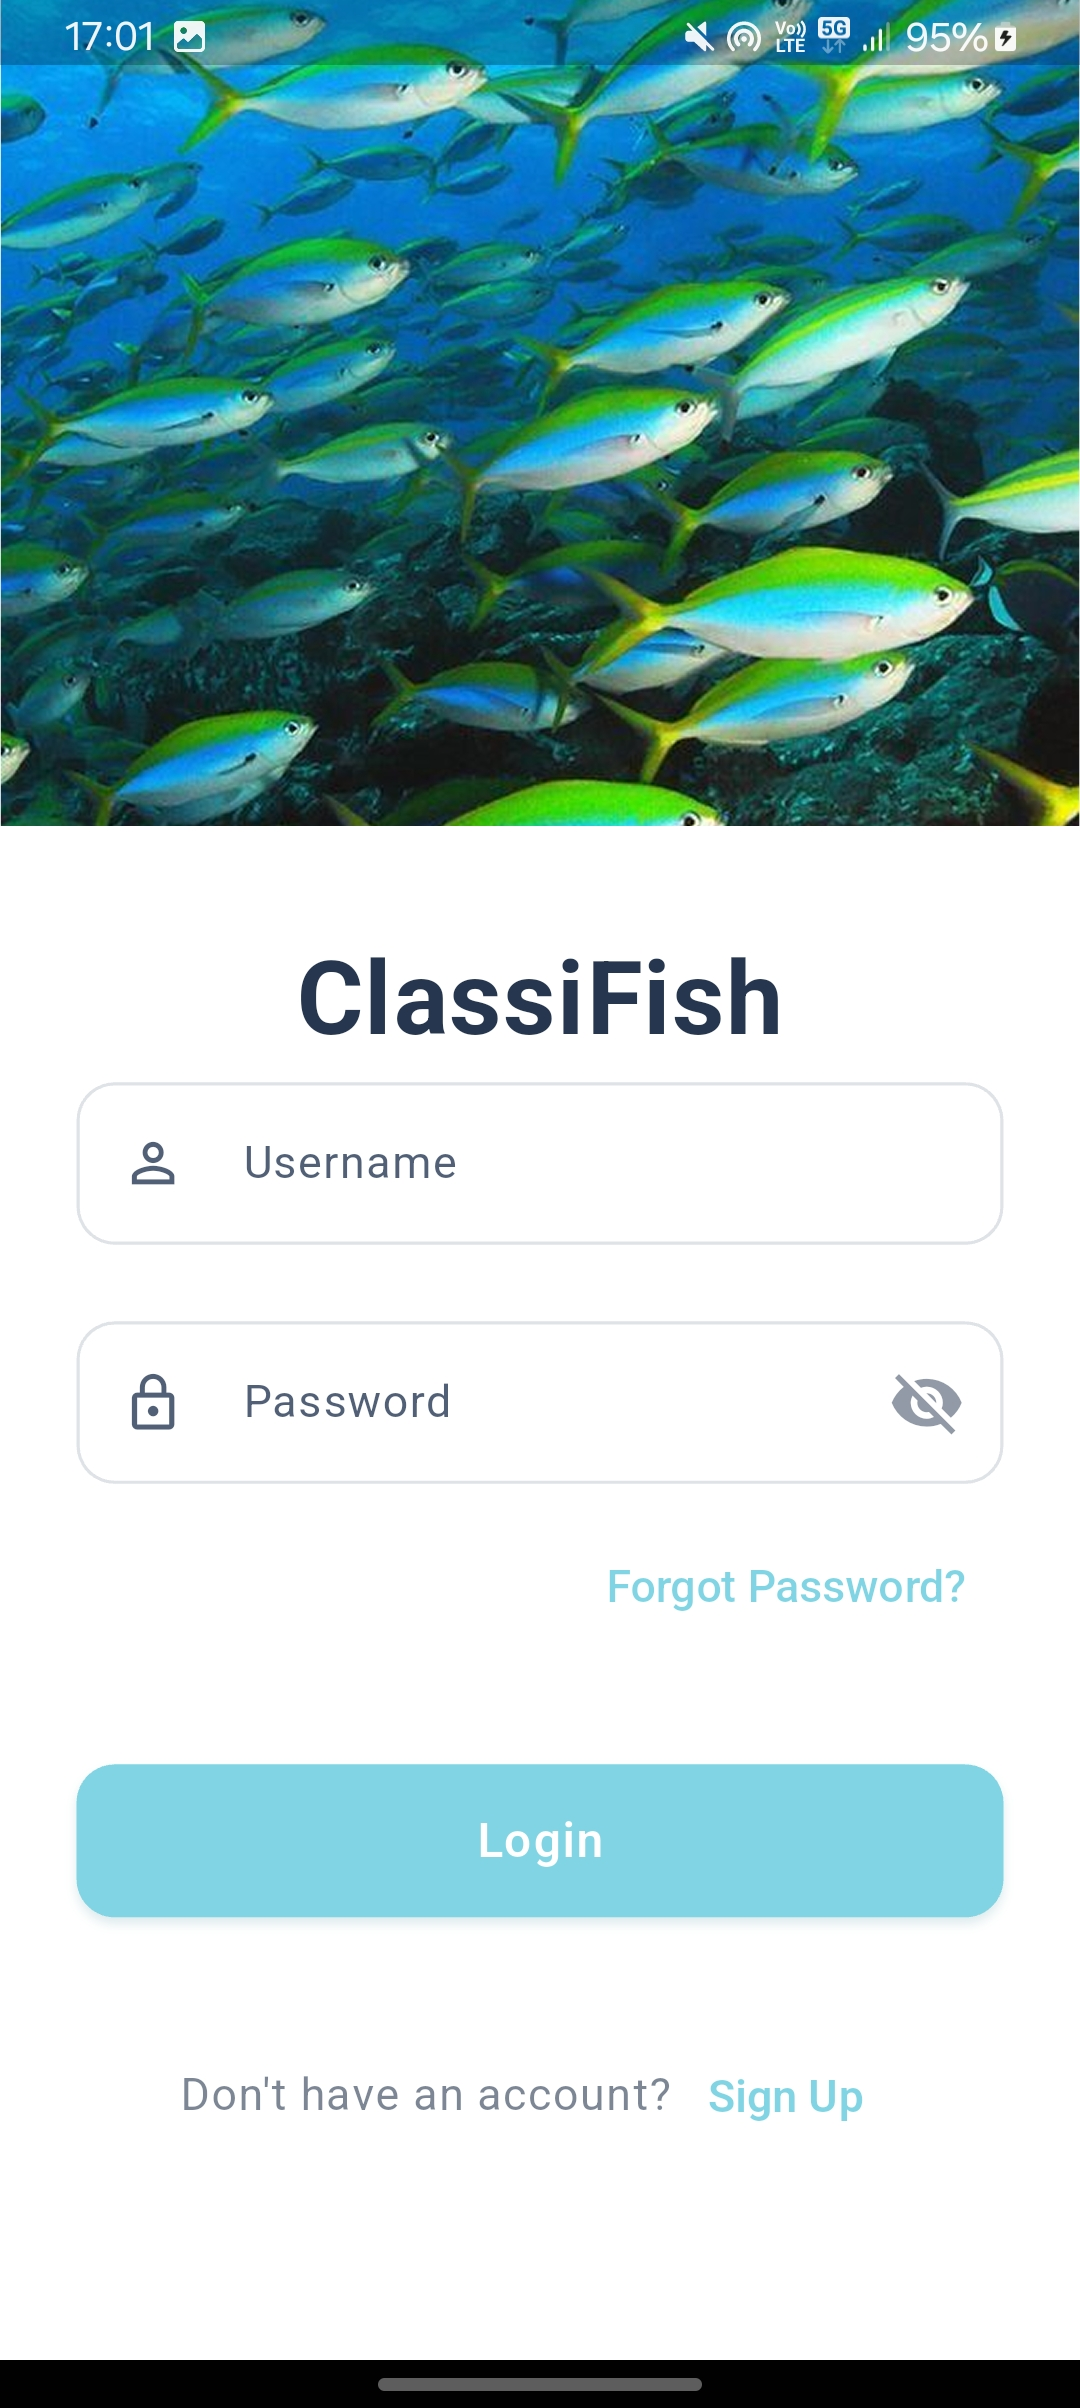
\includegraphics[height=0.5\textheight]{images/images/mobile_app/login.jpg}
        \caption{Login}
    \end{minipage}
    \hfill
    \begin{minipage}[b]{0.48\textwidth}
        \centering
        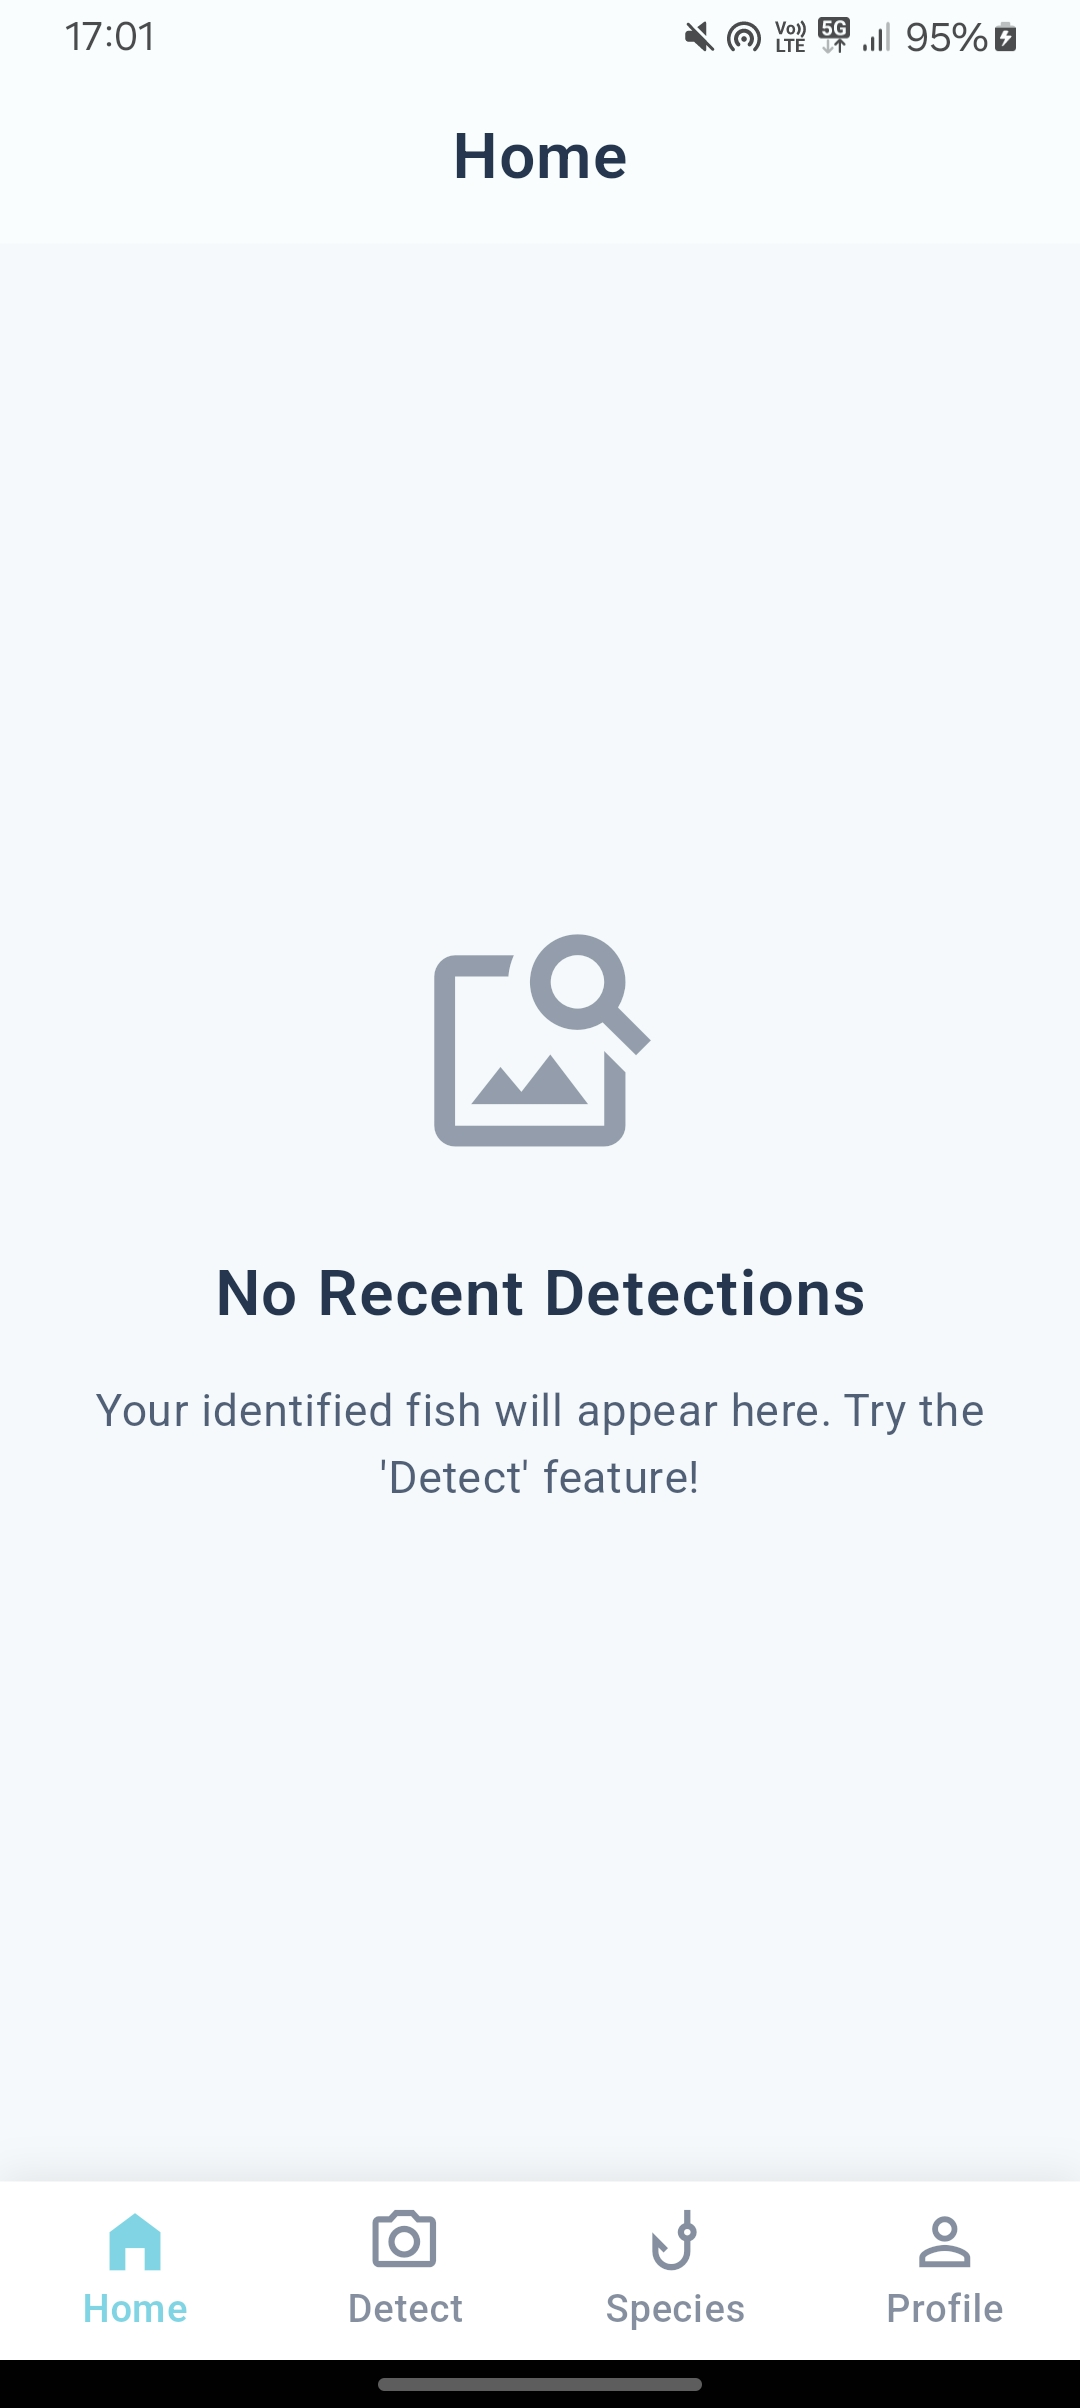
\includegraphics[height=0.5\textheight]{images/images/mobile_app/homescreen(detection history).jpg}
        \caption{Home Screen}
    \end{minipage}
    \end{figure}
    
\subsection{Login and Homepage}
The Login screen allows users to access their account using their registered credentials. Only users with an existing account can proceed through this step. Upon successful login, the user is directed to the Homepage of the mobile application. The homepage contains four main components:

\begin{itemize}
    \item\textbf{Detection Button:} used to initiate the fish species detection feature.
    \item\textbf{Fish Species Button:} opens a list of recognized fish species and in this section you can search fish specie.
    \item\textbf{Profile:} provides access to the user's account information and settings.
\end{itemize}

\pagebreak

\begin{figure}[H]
    \centering
    \begin{minipage}[b]{0.48\textwidth}
        \centering
        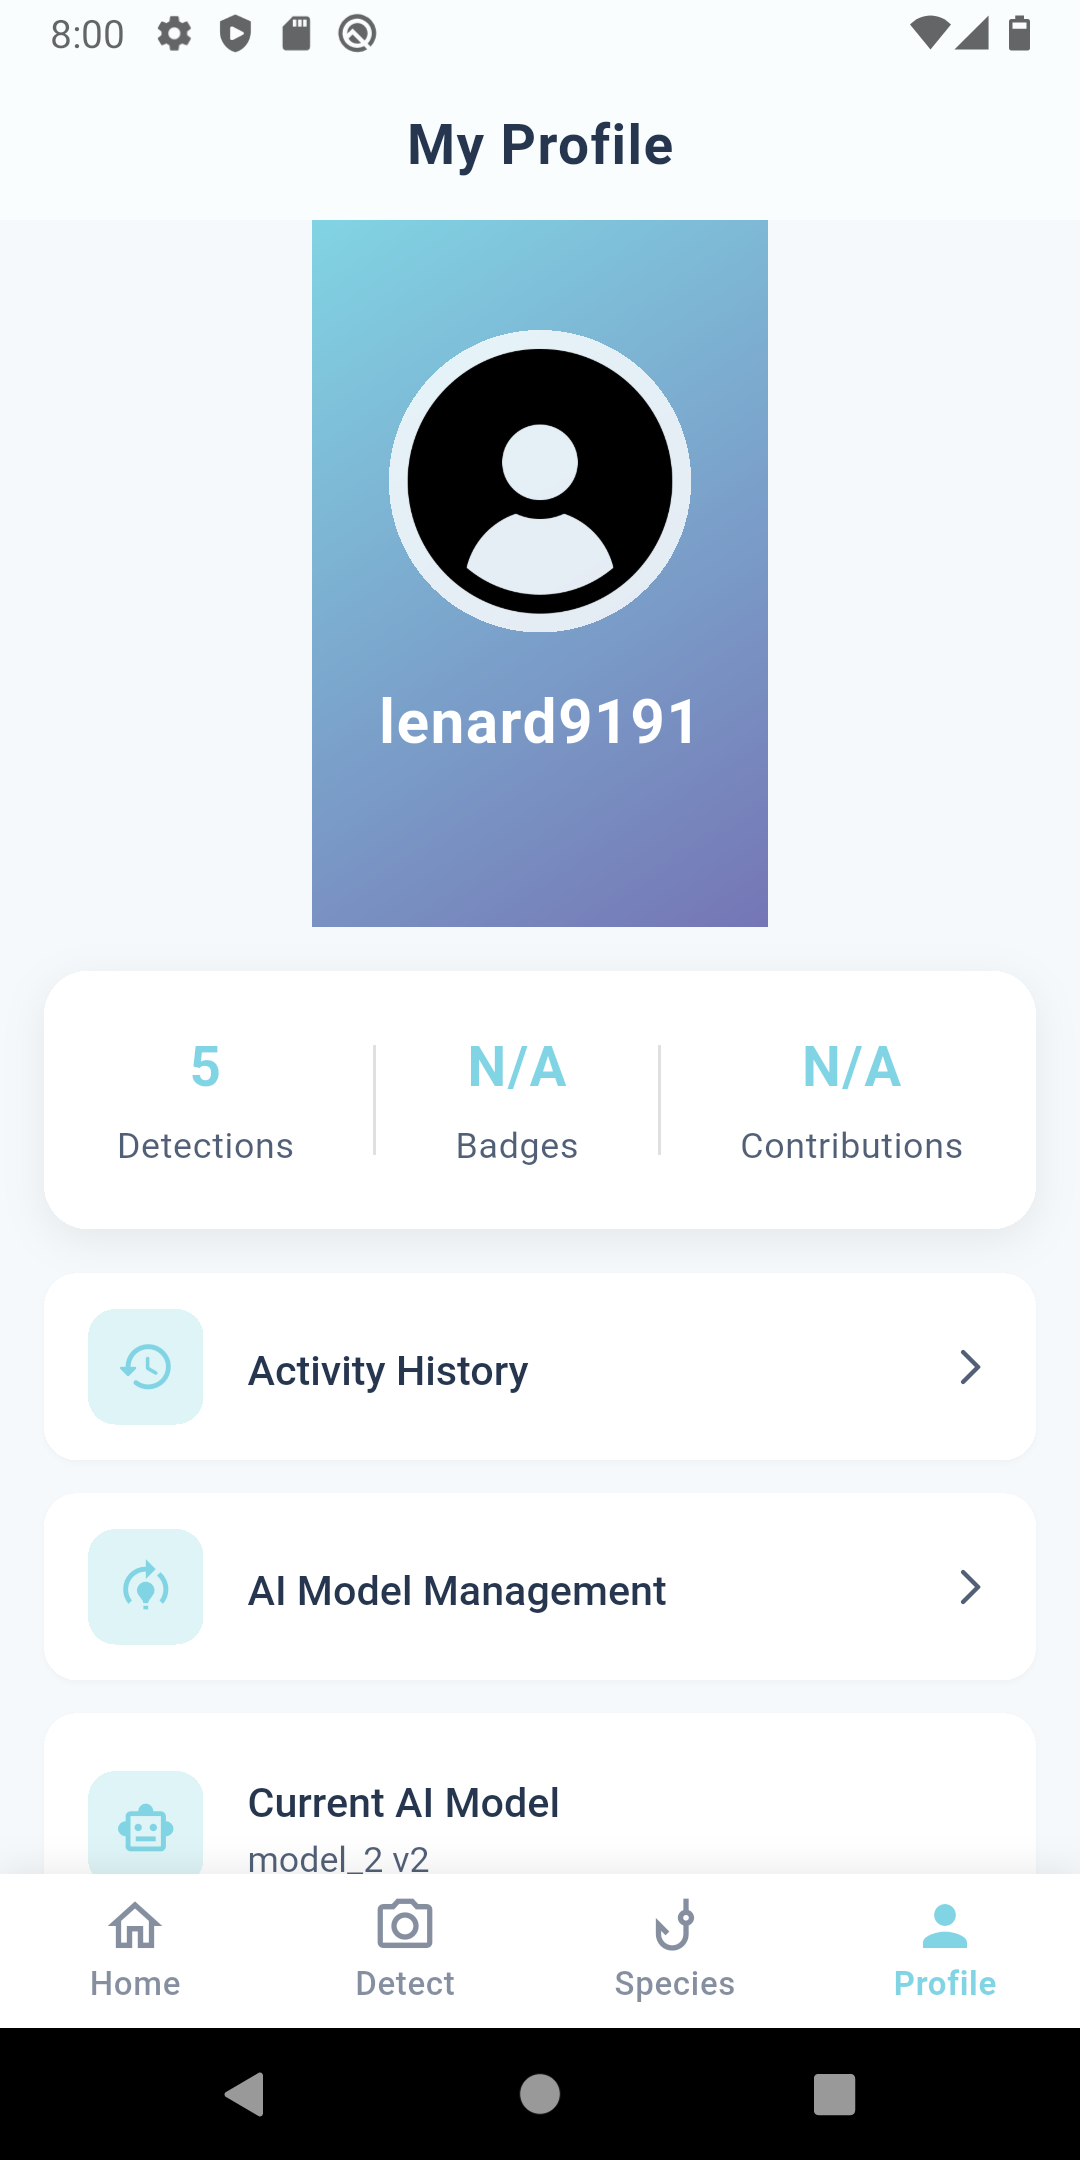
\includegraphics[height=0.5\textheight]{images/images/mobile_app/revision/Profle1.png}
    \end{minipage}
    \hfill
    \begin{minipage}[b]{0.48\textwidth}
        \centering
        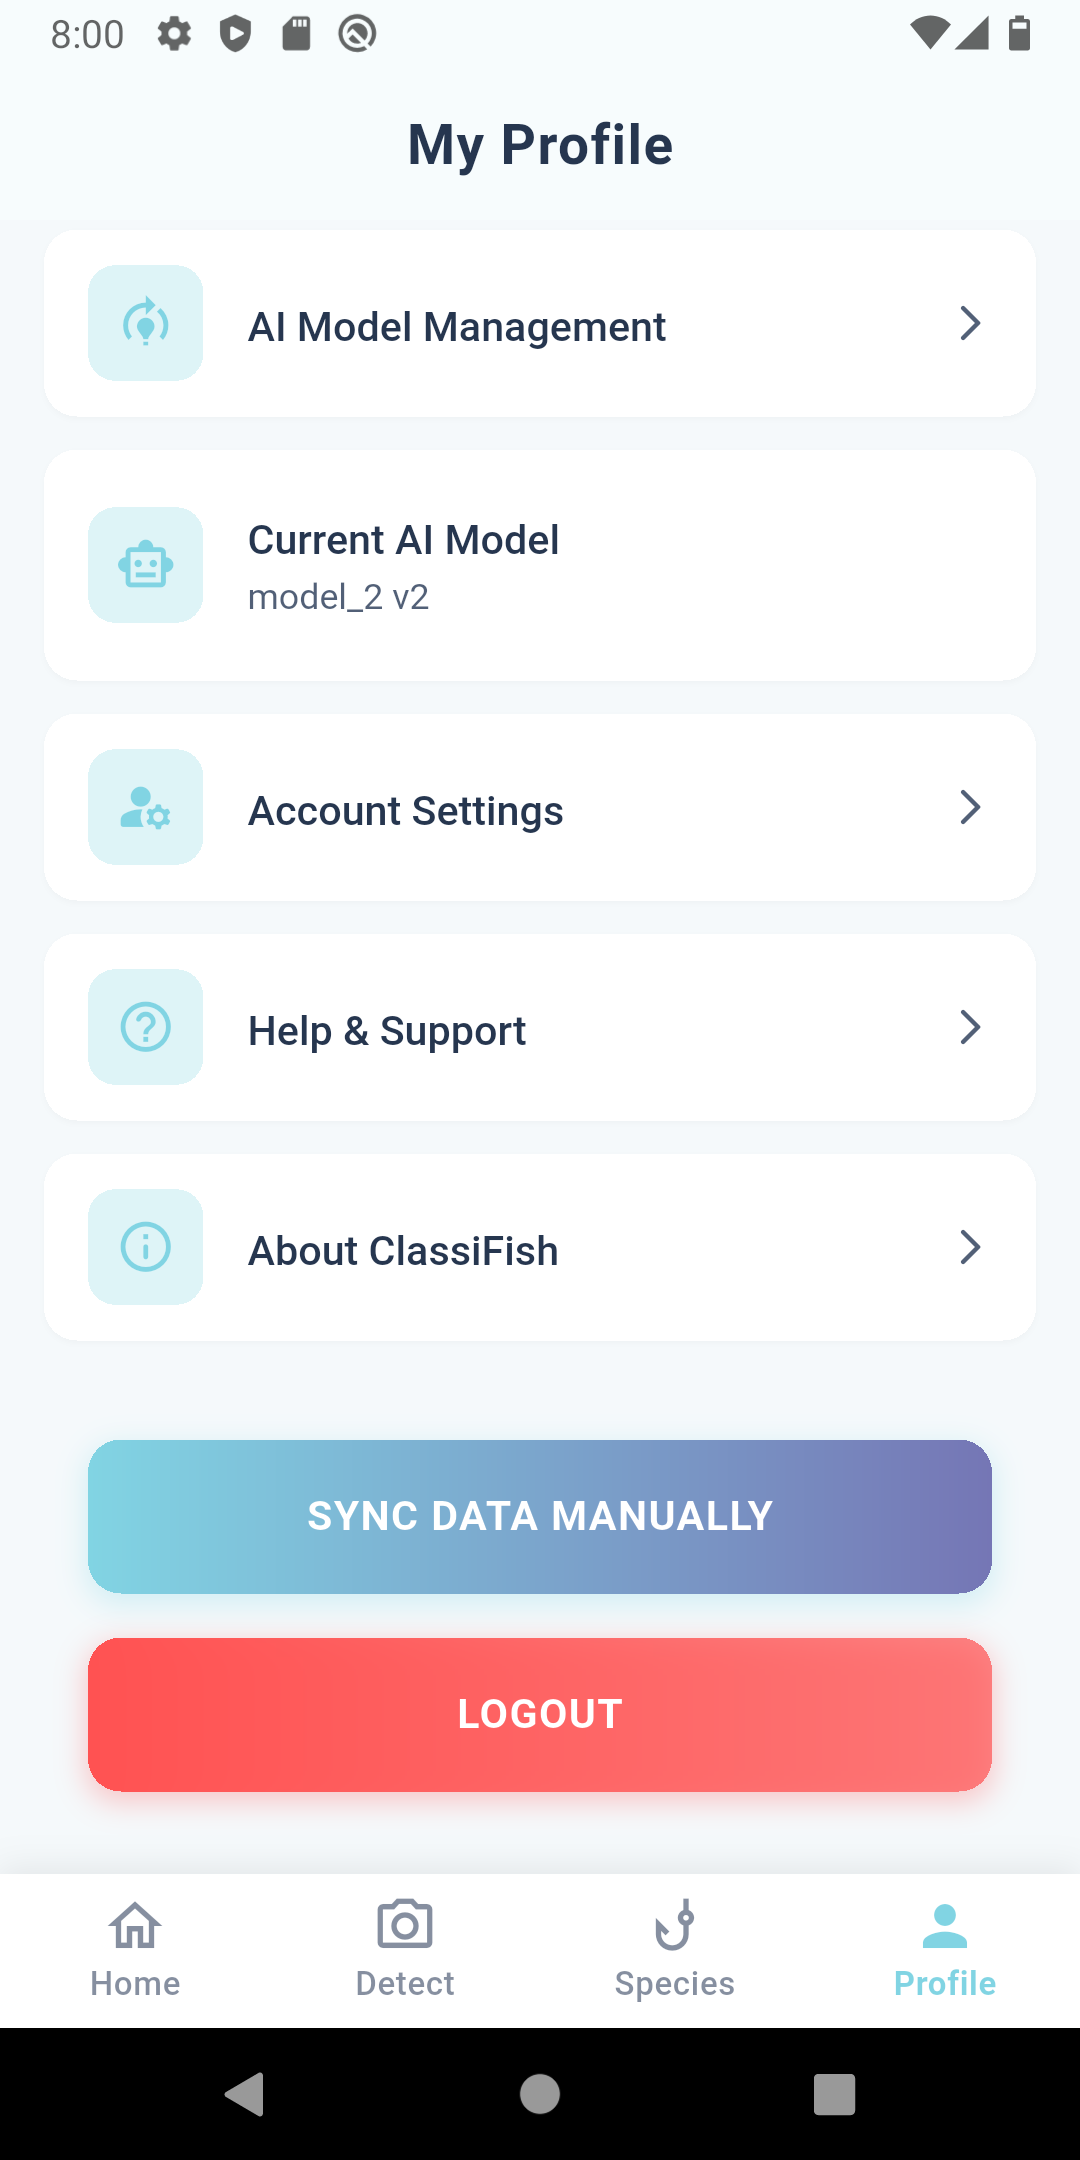
\includegraphics[height=0.5\textheight]{images/images/mobile_app/revision/Profle2.png}
    \end{minipage}
    \caption{User Profile}
\end{figure}

\subsection{User Profile}
The User Profile section provides comprehensive information about the user’s detections, milestones such as badges and contributions, and activity history. It also includes AI model management, details of the current AI model used by the application, account settings, help and support for troubleshooting issues, and a brief overview of the ClassiFish application.
\newpage


 \begin{figure}[H]
       \begin{minipage}[b]{0.48\textwidth}
        \centering
        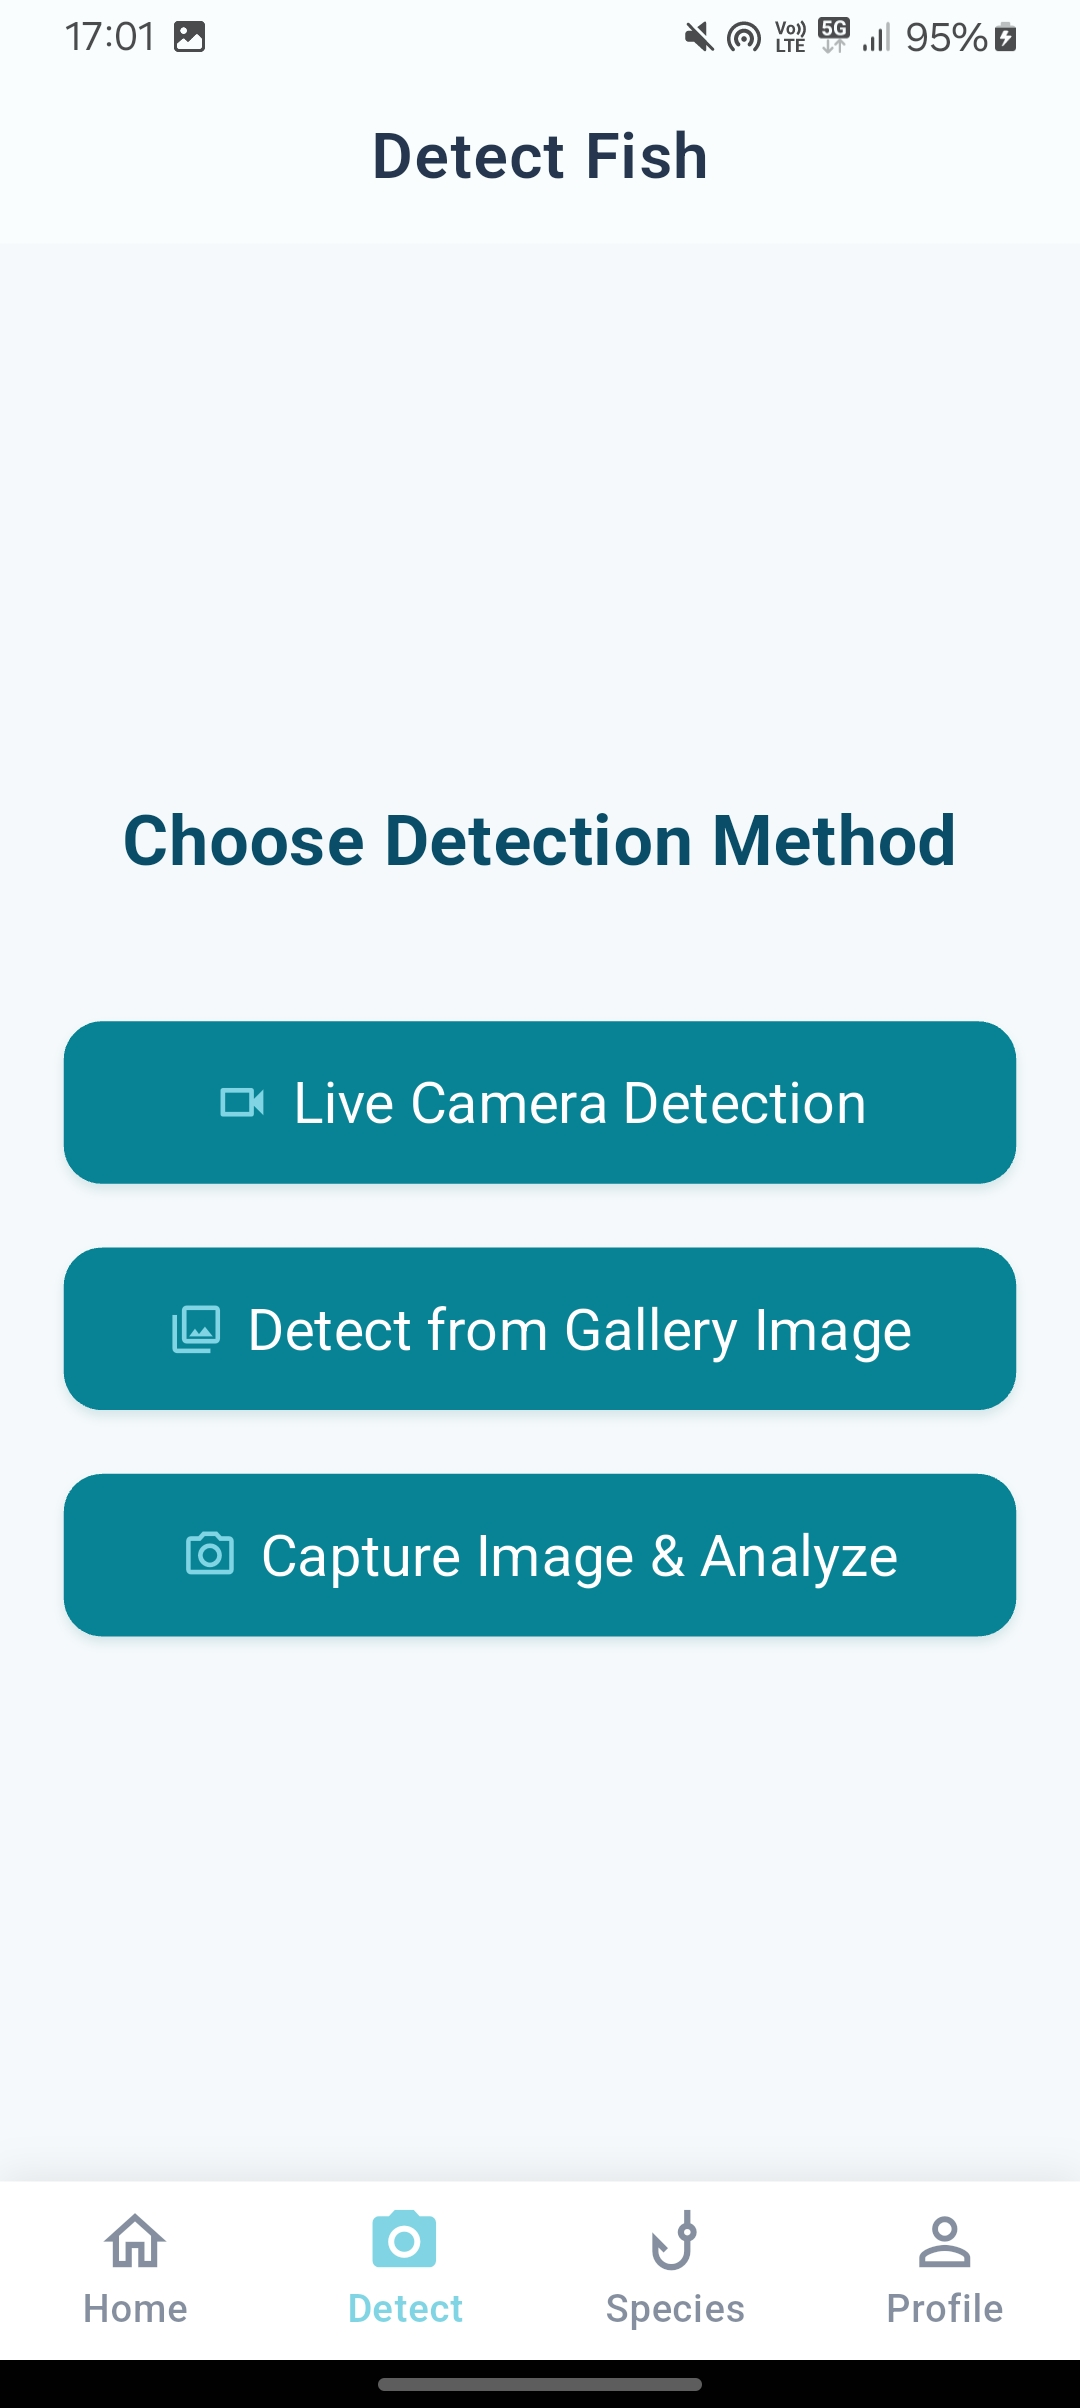
\includegraphics[height=0.5\textheight]{images/images/mobile_app/detectionscreen(choose 3).jpg}
        \caption{Choose Detection Method}}
    \end{minipage}
    \hfill
        \begin{minipage}[b]{0.48 \textwidth}
        \centering
        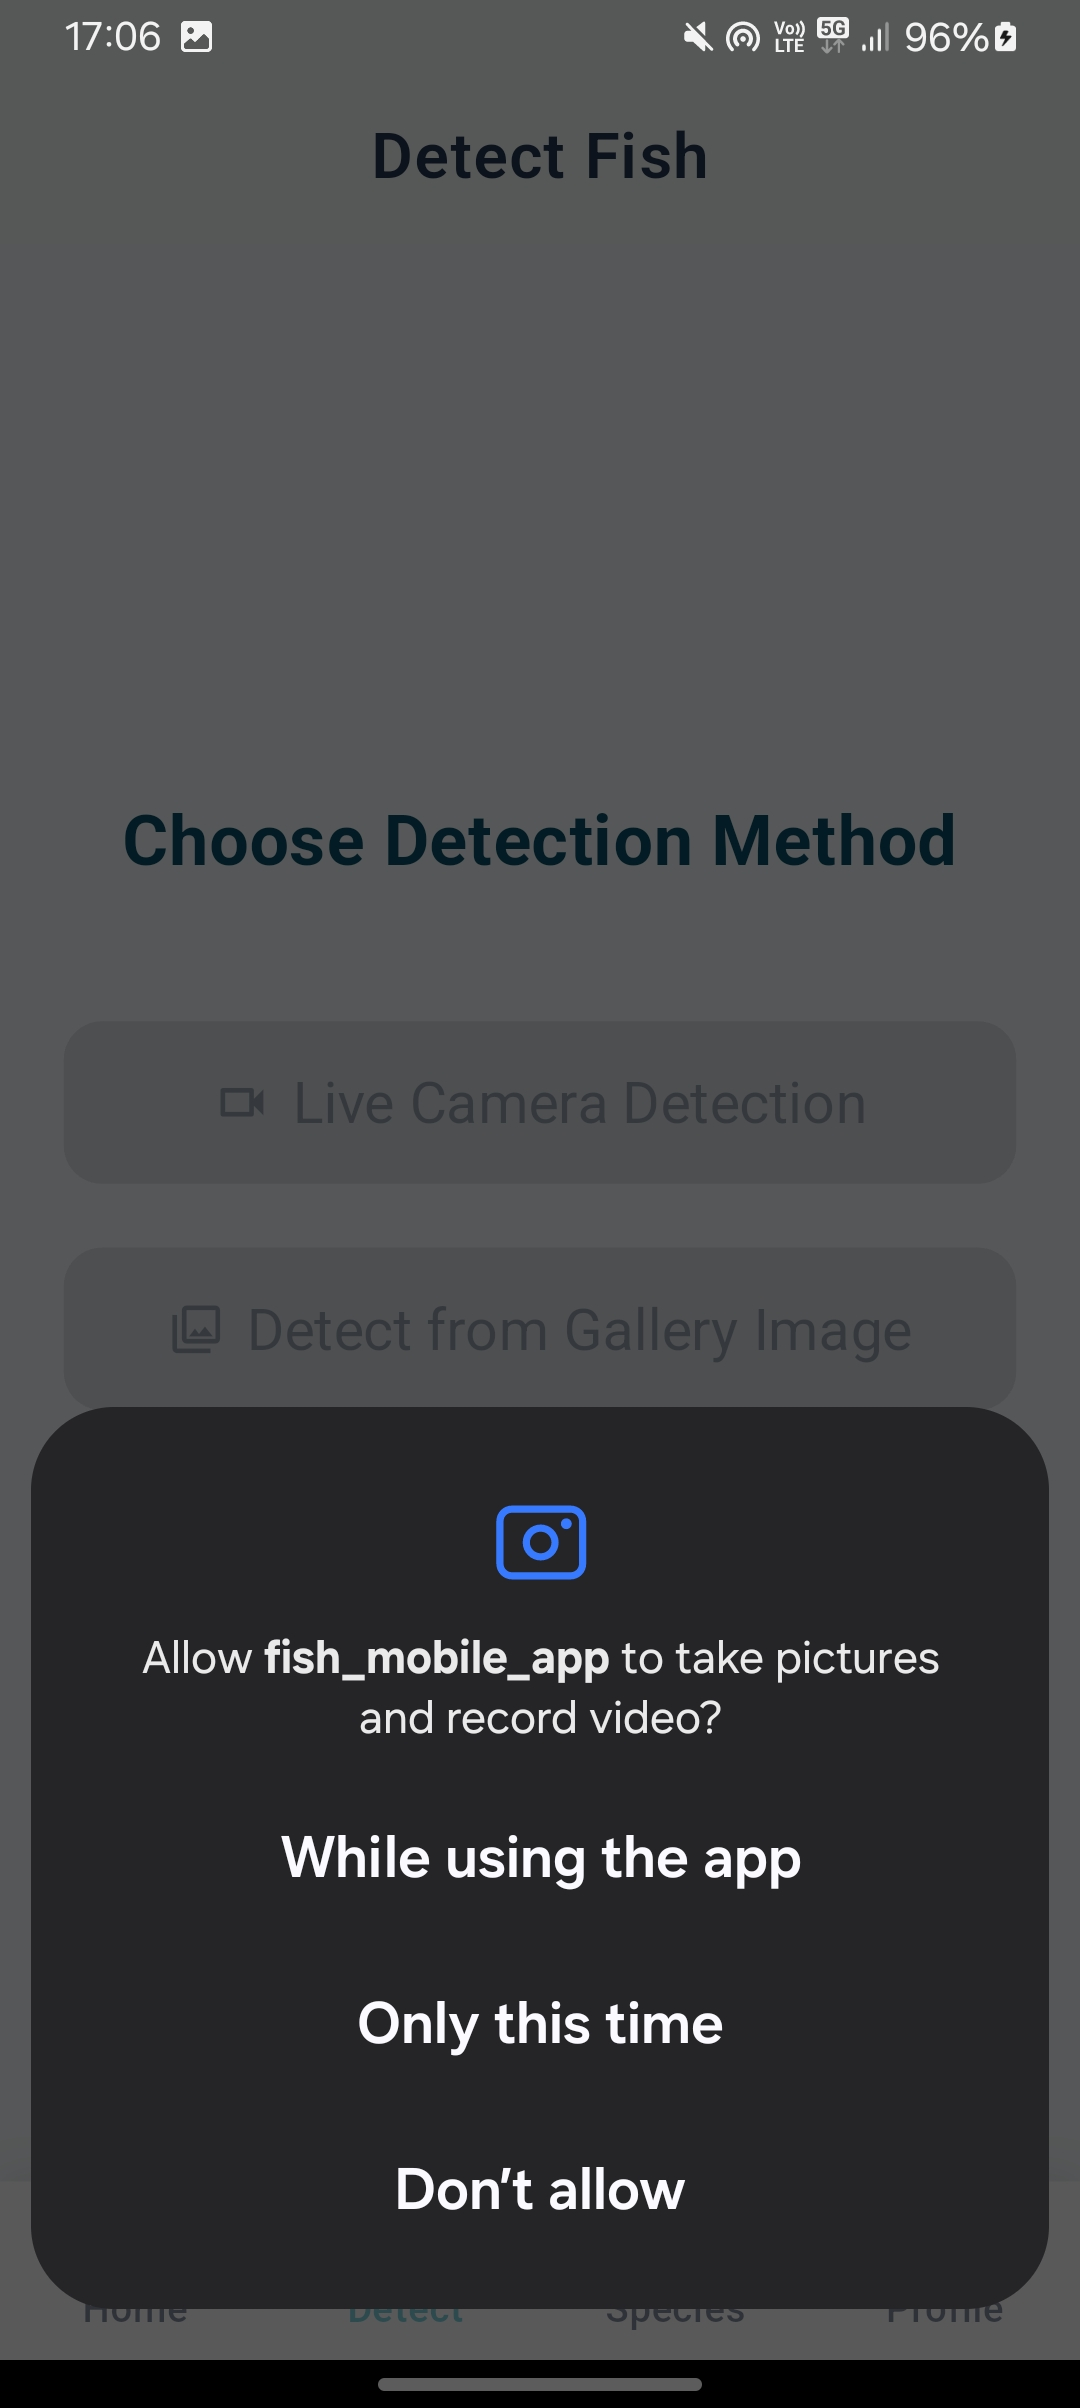
\includegraphics[height=0.5\textheight]
        {images/images/mobile_app/Permissions.jpg}
        \caption{User Permission}
    \end{minipage}
    \end{figure}

\subsection{Fish Detection Features}
When the Detection button is selected from the homepage, the application requests user permission to access the device’s camera and storage. The user must grant permission to proceed with the detection process. After permission is granted, the application presents three detection methods:

\begin{itemize}
    \item\textbf{Live Detection:} uses the device’s camera to identify fish species in real-time.

    \item\textbf{Detect from Gallery Image:} allows the user to select an existing image from their device’s gallery for analysis.
    \item\textbf{Capture Image and Analyze:} enables the user to take a new photo using the camera, which is then analyzed by the application.
\end{itemize}


\pagebreak

 \begin{figure}[H]
       \begin{minipage}[b]{0.48\textwidth}
    \centering
        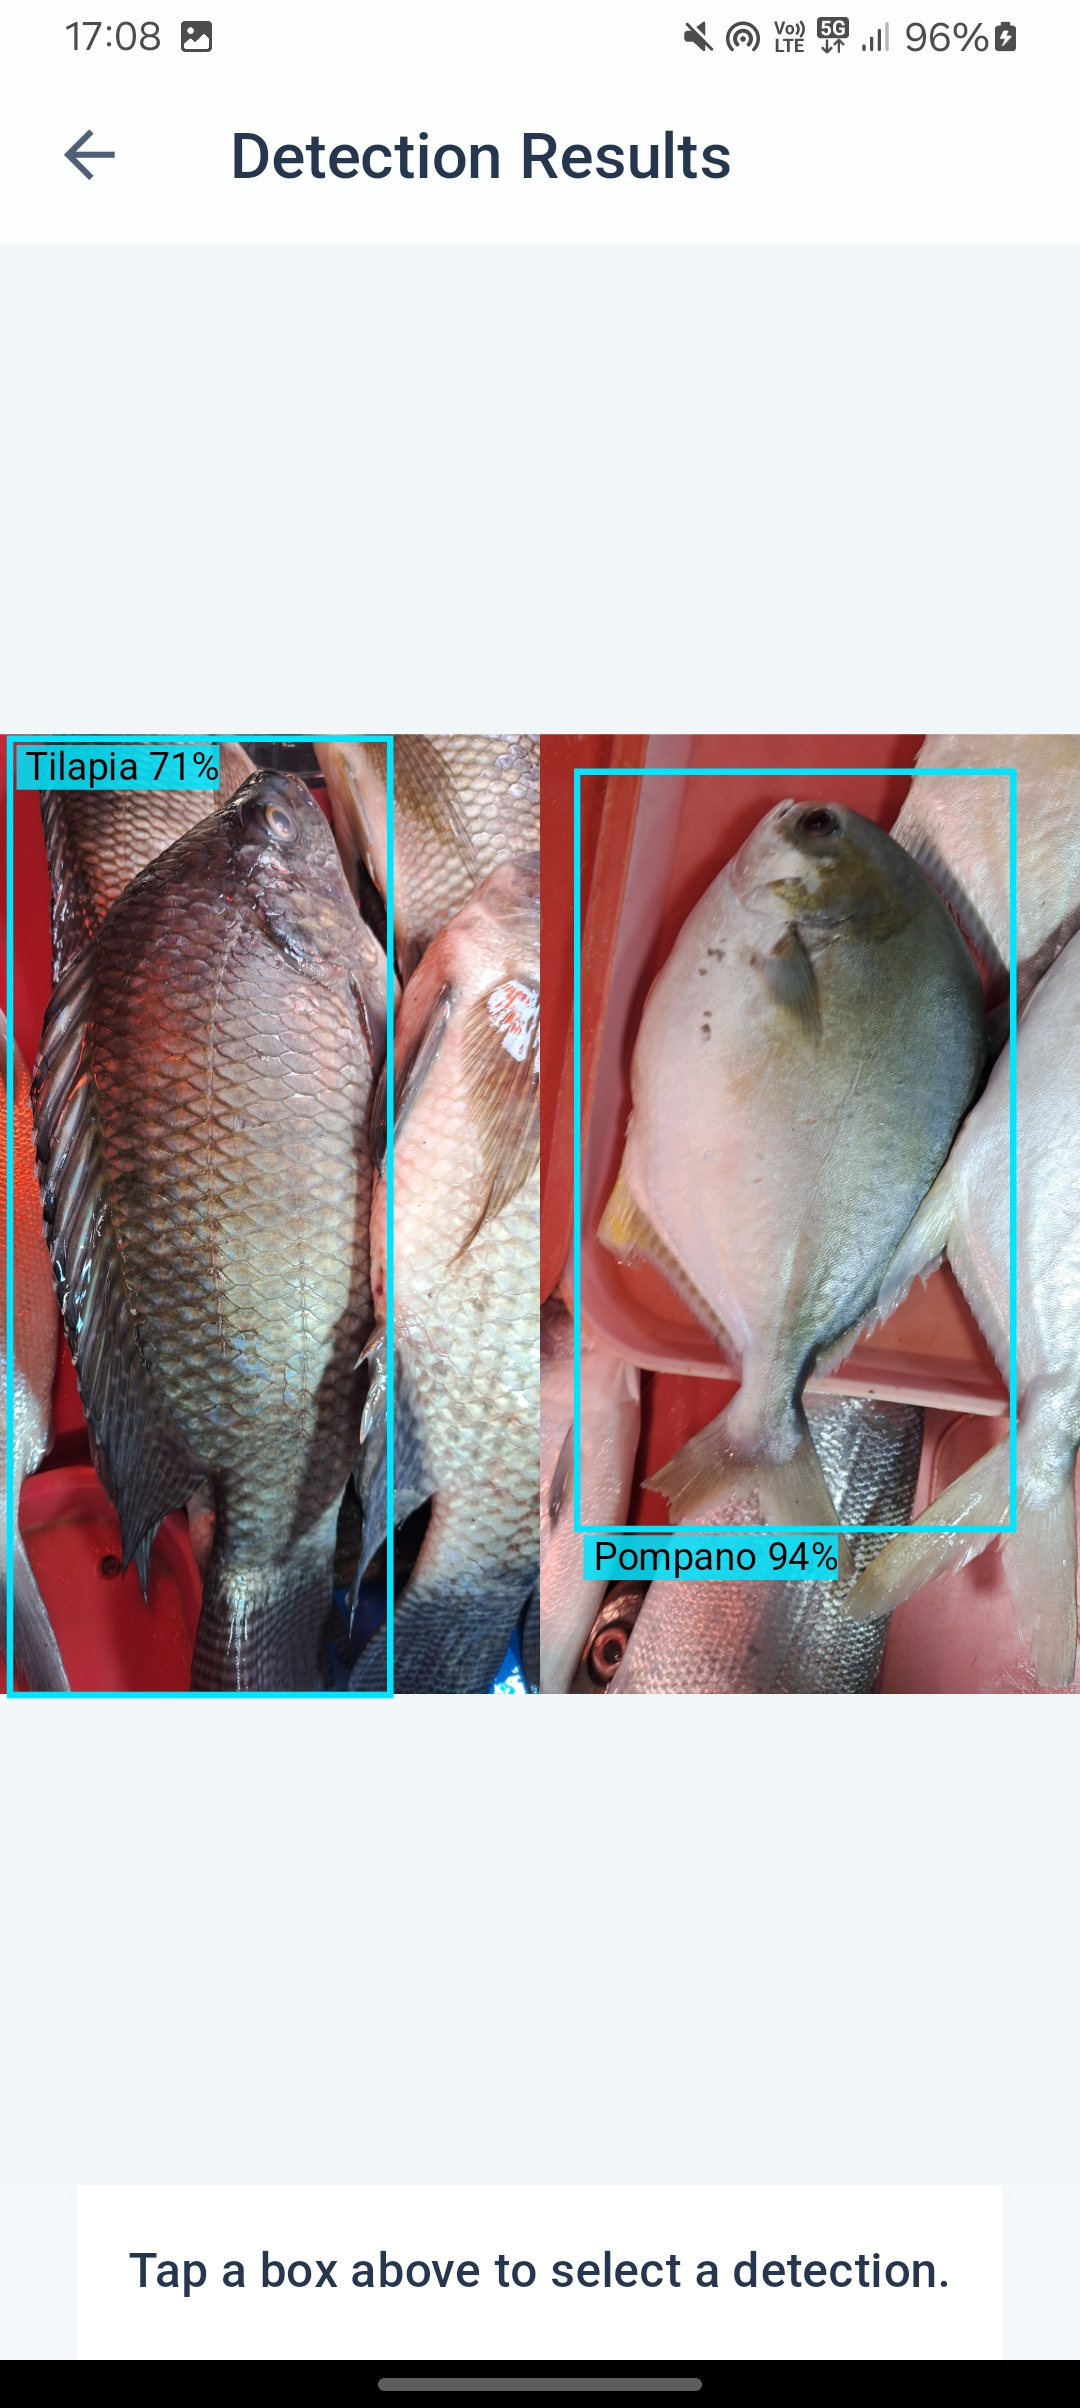
\includegraphics[height=0.5\textheight]{images/images/mobile_app/DetectionResults.jpg}
        \caption{Fish Detection}
    \end{minipage}
    \hfill
    \begin{minipage}[b]{0.48\textwidth}
     \centering
        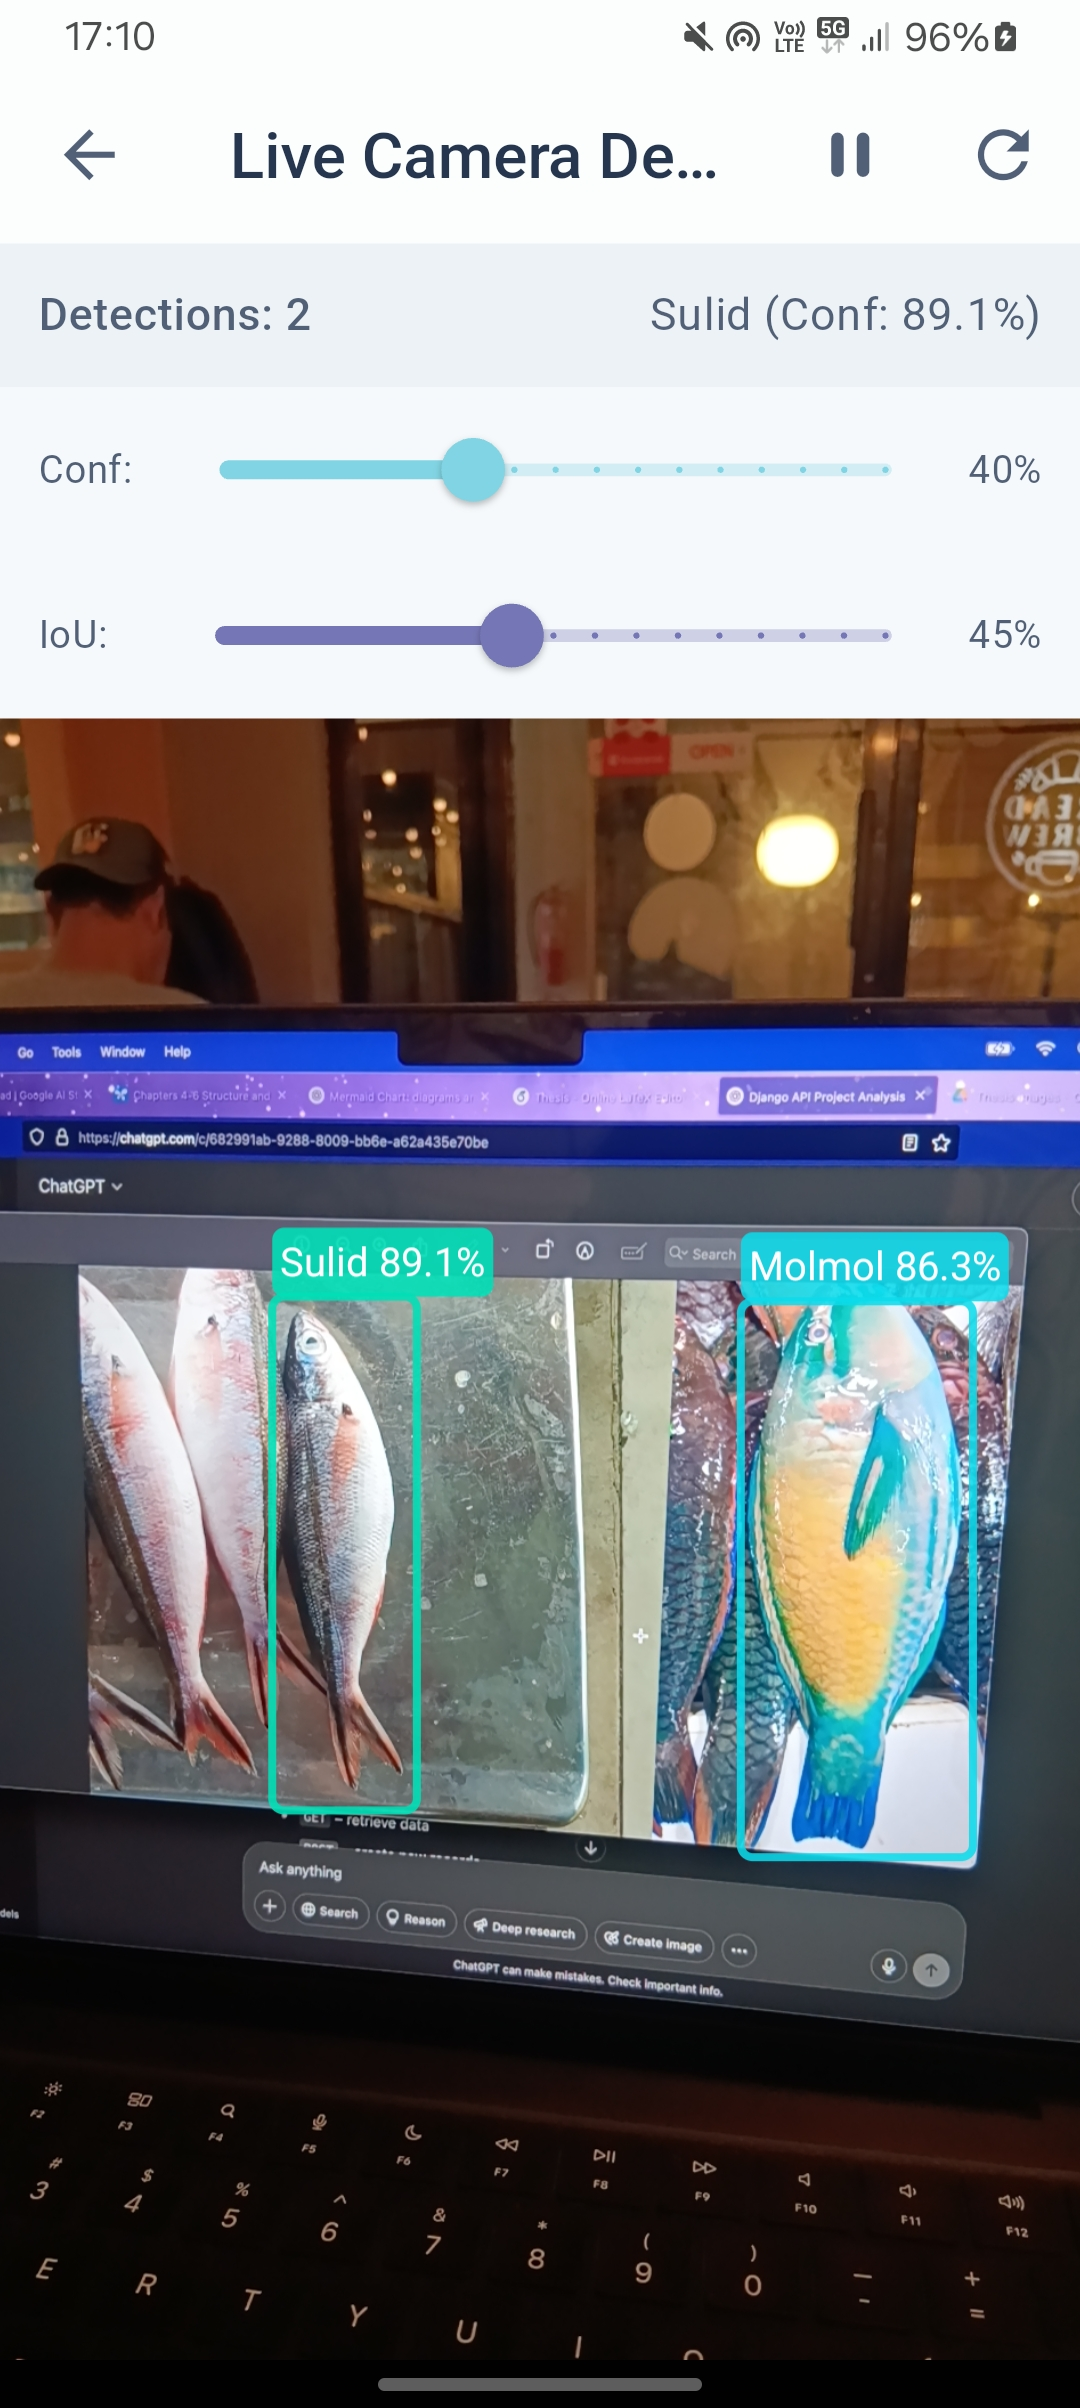
\includegraphics[height=0.5\textheight]{images/images/mobile_app/LiveCameraScreen.jpg}
        \caption{Real-Time Detection}
    \end{minipage}
    \end{figure}
    
\subsubsection{Detection Results}
After the detection process is completed, the application displays the result by overlaying a bounding box around the detected fish in the image. Each bounding box includes a label indicating the identified fish species.

For real-time detection, the application continuously analyzes the live camera feed and displays bounding boxes and corresponding species labels in real-time as fish are detected. This feature allows users to instantly recognize fish species as they appear in view.

\pagebreak

 \begin{figure}[H]
       \begin{minipage}[b]{0.48\textwidth}
        \centering
        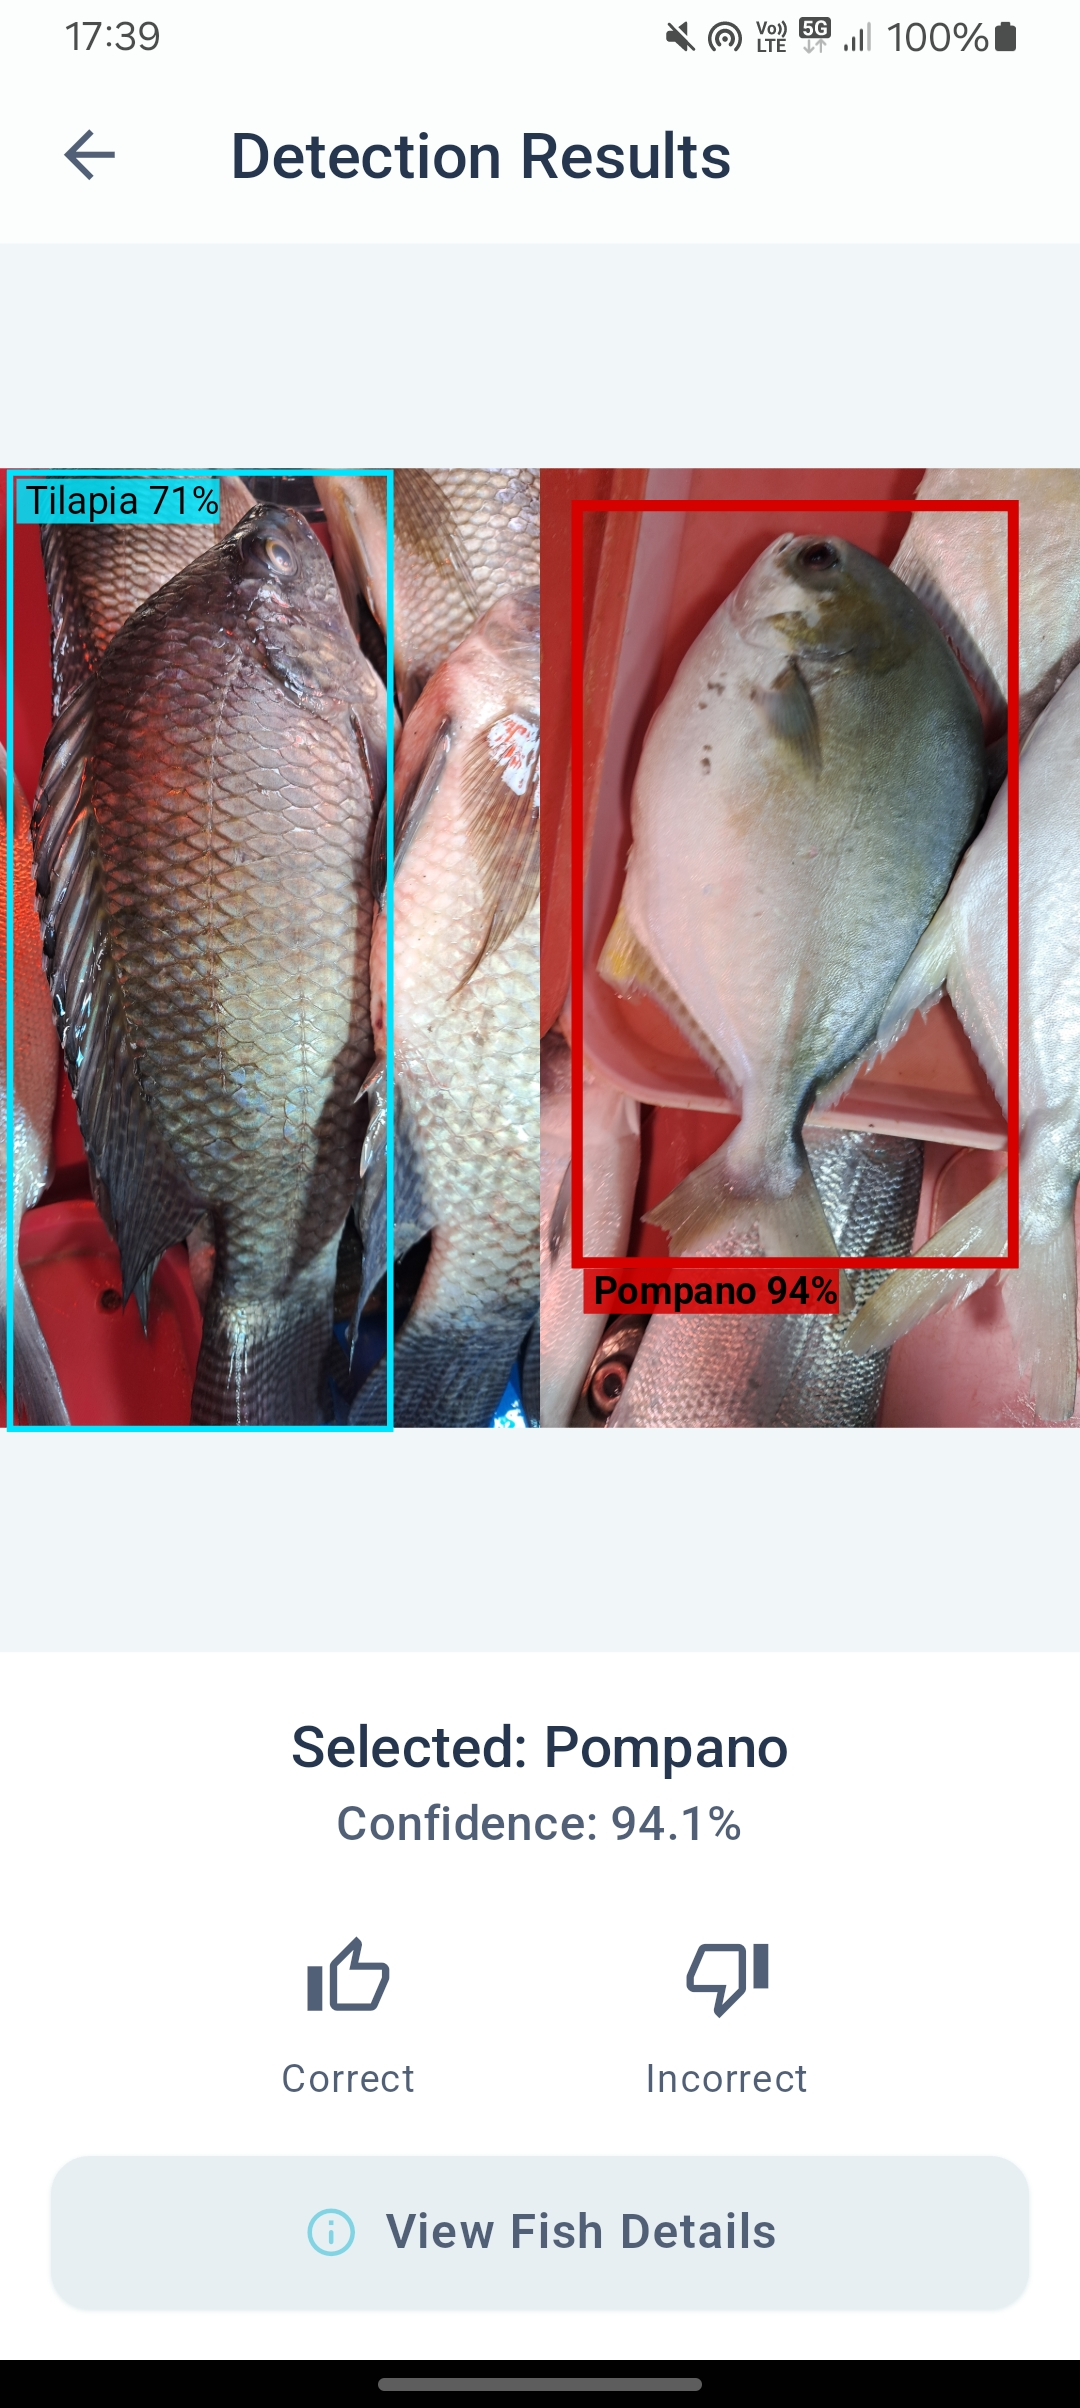
\includegraphics[height=0.5\textheight]{images/images/mobile_app/ResultClickBoundingBox.jpg}
        \caption{Choose Correct and Incorrect Feedback}
    \end{minipage}
    \hfill
    \begin{minipage}[b]{0.48\textwidth}
        \centering
        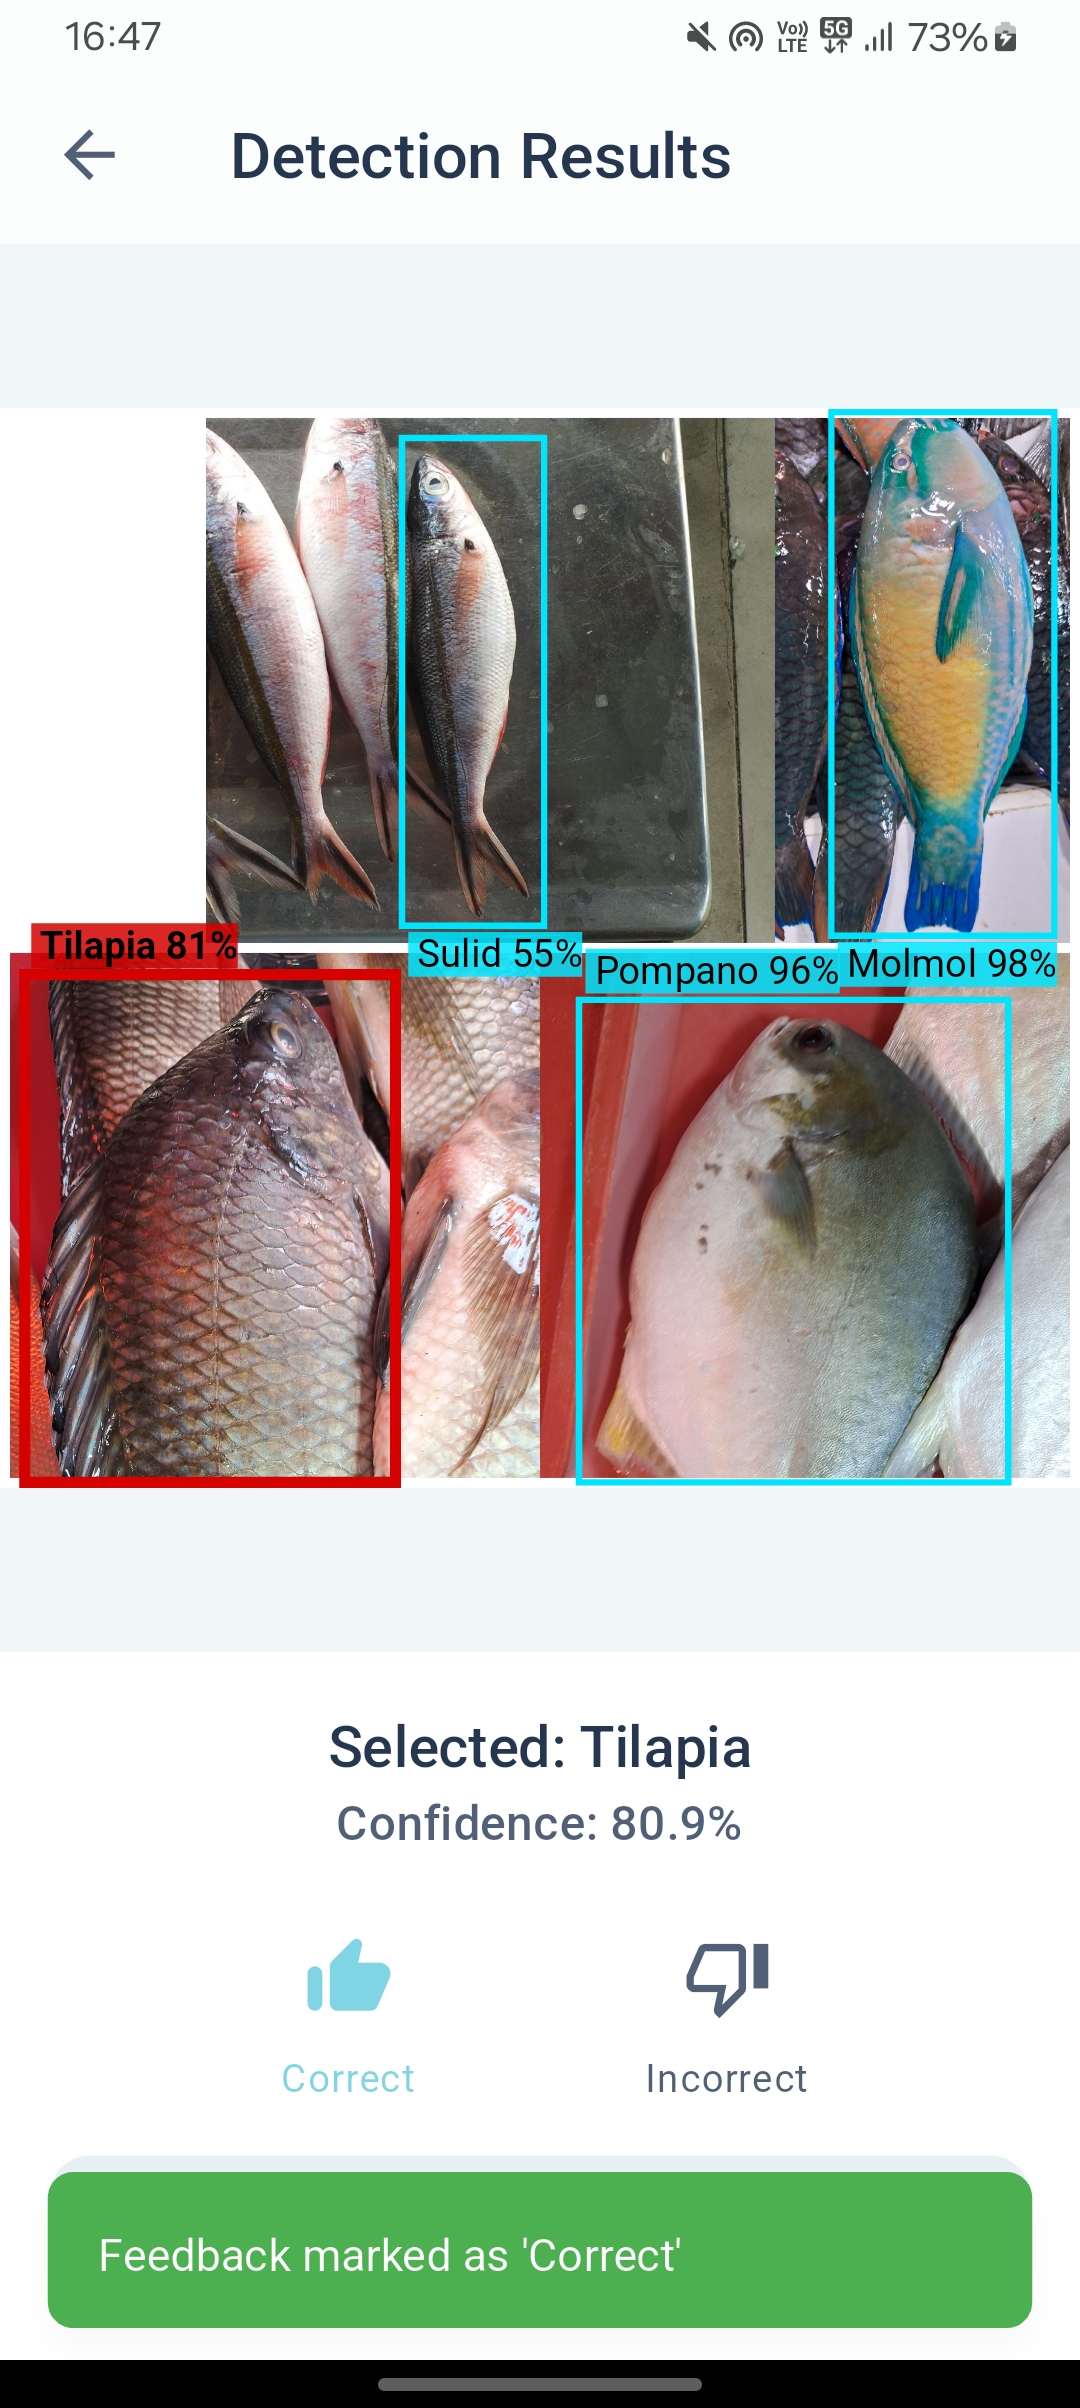
\includegraphics[height=0.5\textheight]{images/images/mobile_app/correct_detection.jpg}
        \caption{Correct Feedback}
    \end{minipage}
    \end{figure}

\subsection{Post-Detection Interaction}
Following detection, the fish species are displayed with bounding boxes and corresponding labels. Users can select a specific fish by tapping on its bounding box. After selecting what fish specie in the image, the users can provide feedback on the detection accuracy by choosing either a thumbs up or thumbs down on that specified fish specie. A thumbs up indicates that the detected fish species is correct, while a thumbs down signifies that the detection is incorrect. This feedback will help to improve the accuracy and reliability of the detection system.

 \begin{figure}[H]
       \begin{minipage}[b]{0.48\textwidth}
        \centering
        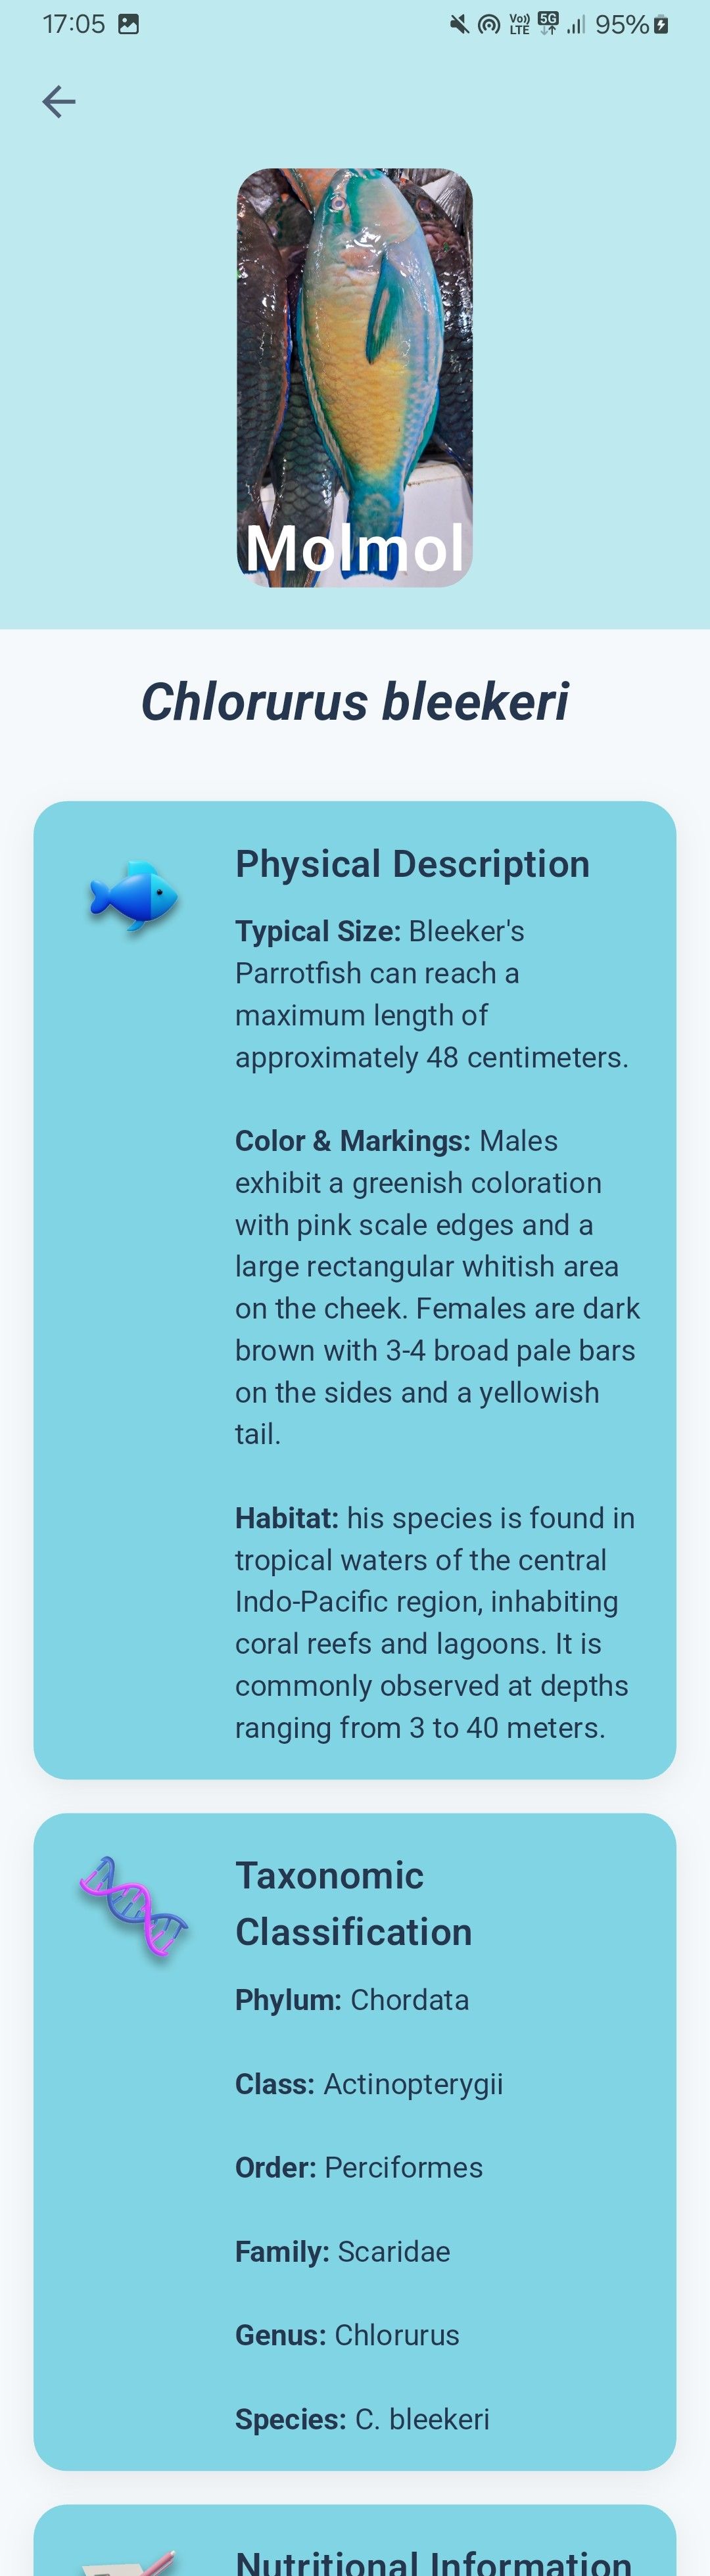
\includegraphics[height=0.6\textheight]{images/images/mobile_app/FIshDetails.jpg}
        \caption{Fish Information}
    \end{minipage}
    \hfill
    \begin{minipage}[b]{0.48\textwidth}
        \centering
        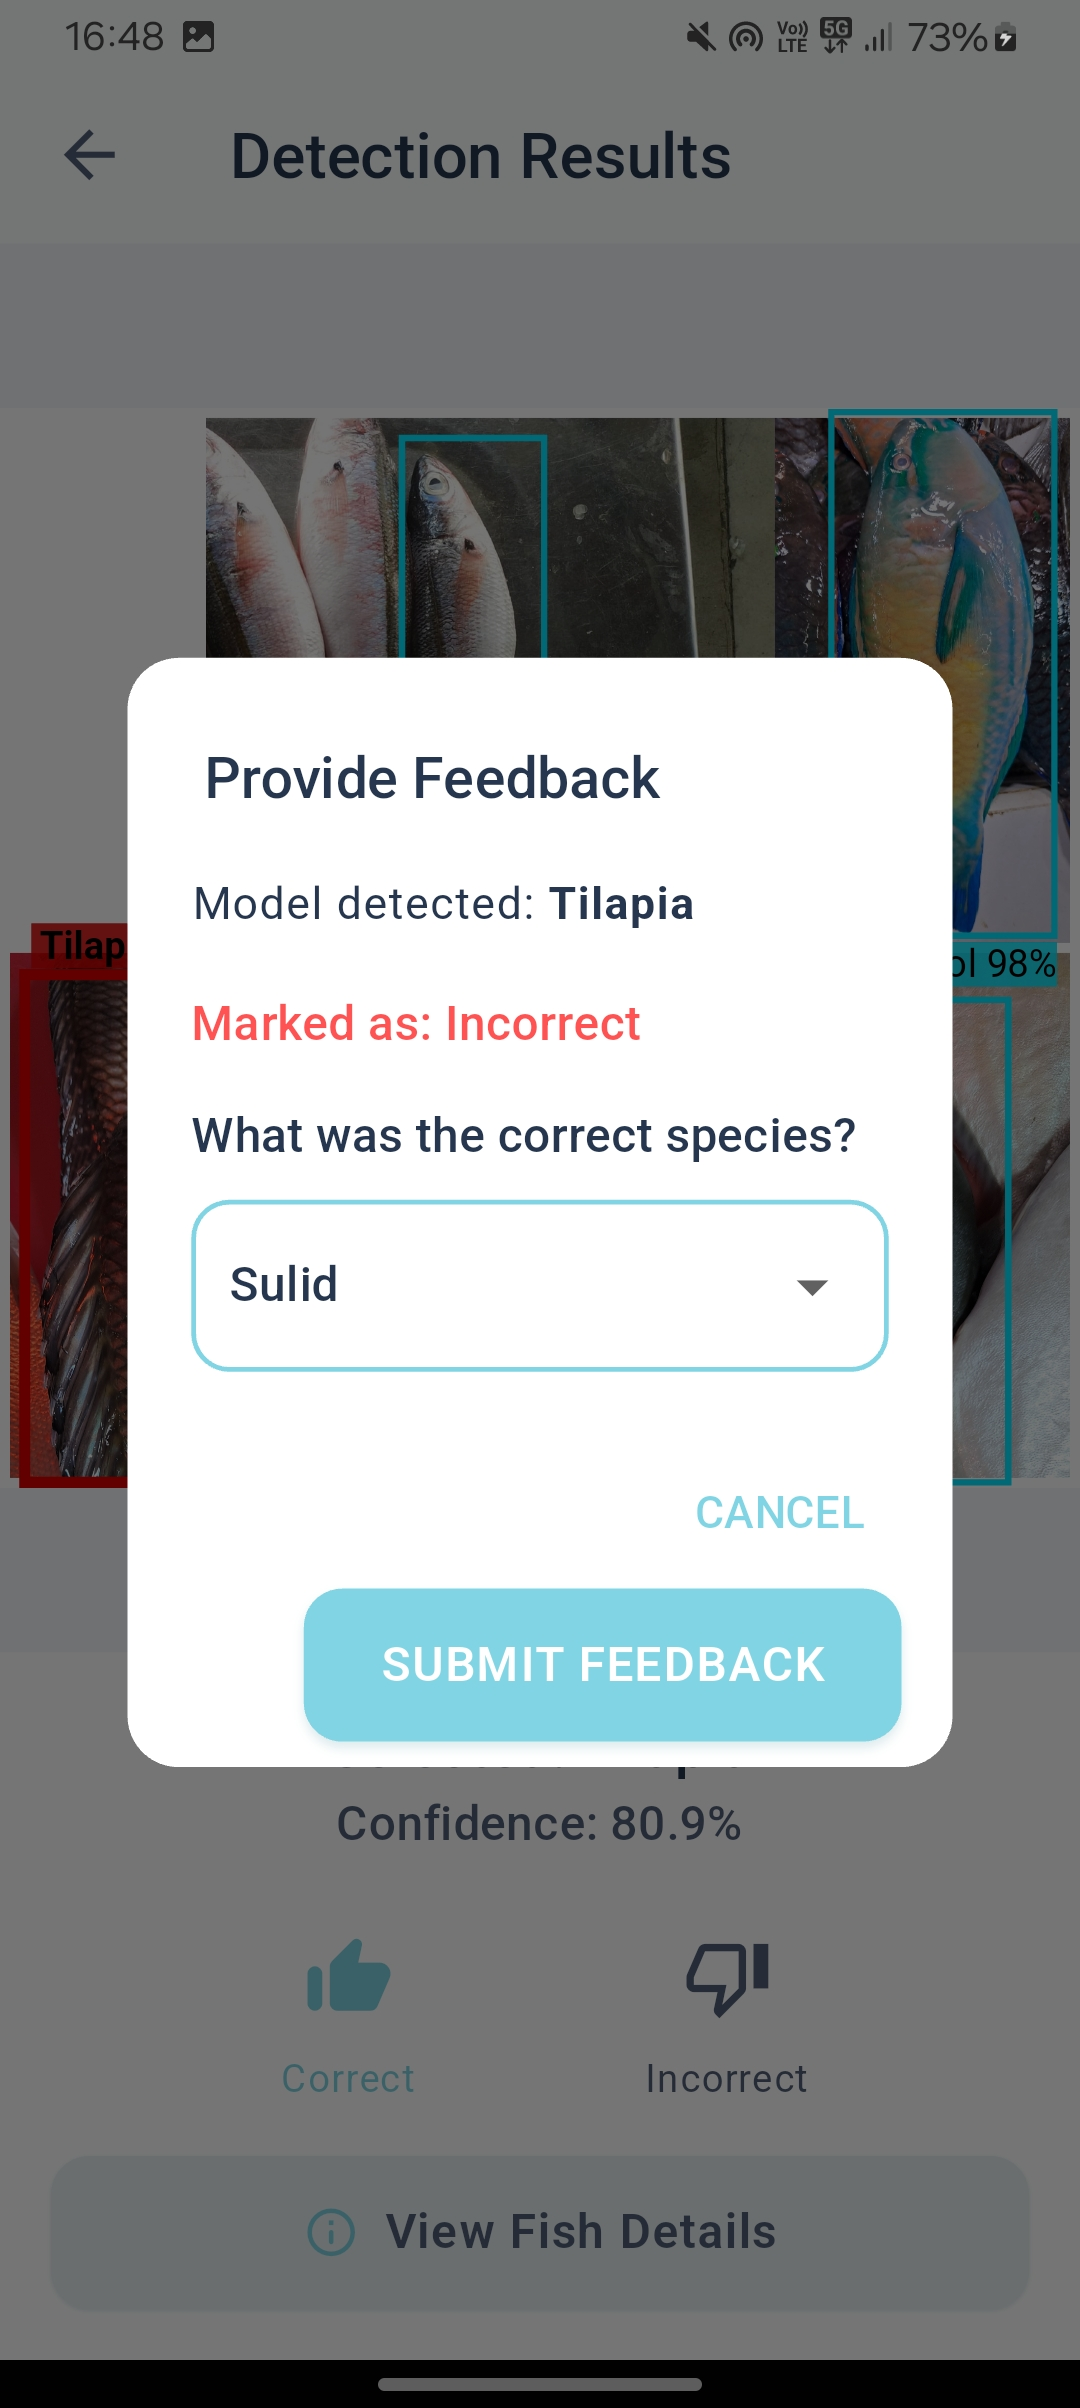
\includegraphics[height=0.6\textheight]{images/images/mobile_app/Select_Option.jpg}
        \caption{Incorrect Feedback and Select Correct Fish Specie}
    \end{minipage}
    \end{figure}


\subsection{Fish Details and Feedback Correction}
Below the detected fish and feedback options, users can choose to view detailed information about the selected fish species by accessing the Fish Details section. This provides relevant data related to the fish. If the user indicates the detection is incorrect by selecting thumbs down, the application prompts the user to complete a feedback form. This form allows the user to select the correct fish species from a scrollable list of options. The user also has the option to cancel the feedback submission if desired. This process helps improve the accuracy of the detection system by collecting corrective input from users.
\newpage

 \begin{figure}[H]
       \begin{minipage}[b]{0.48\textwidth}
        \centering
        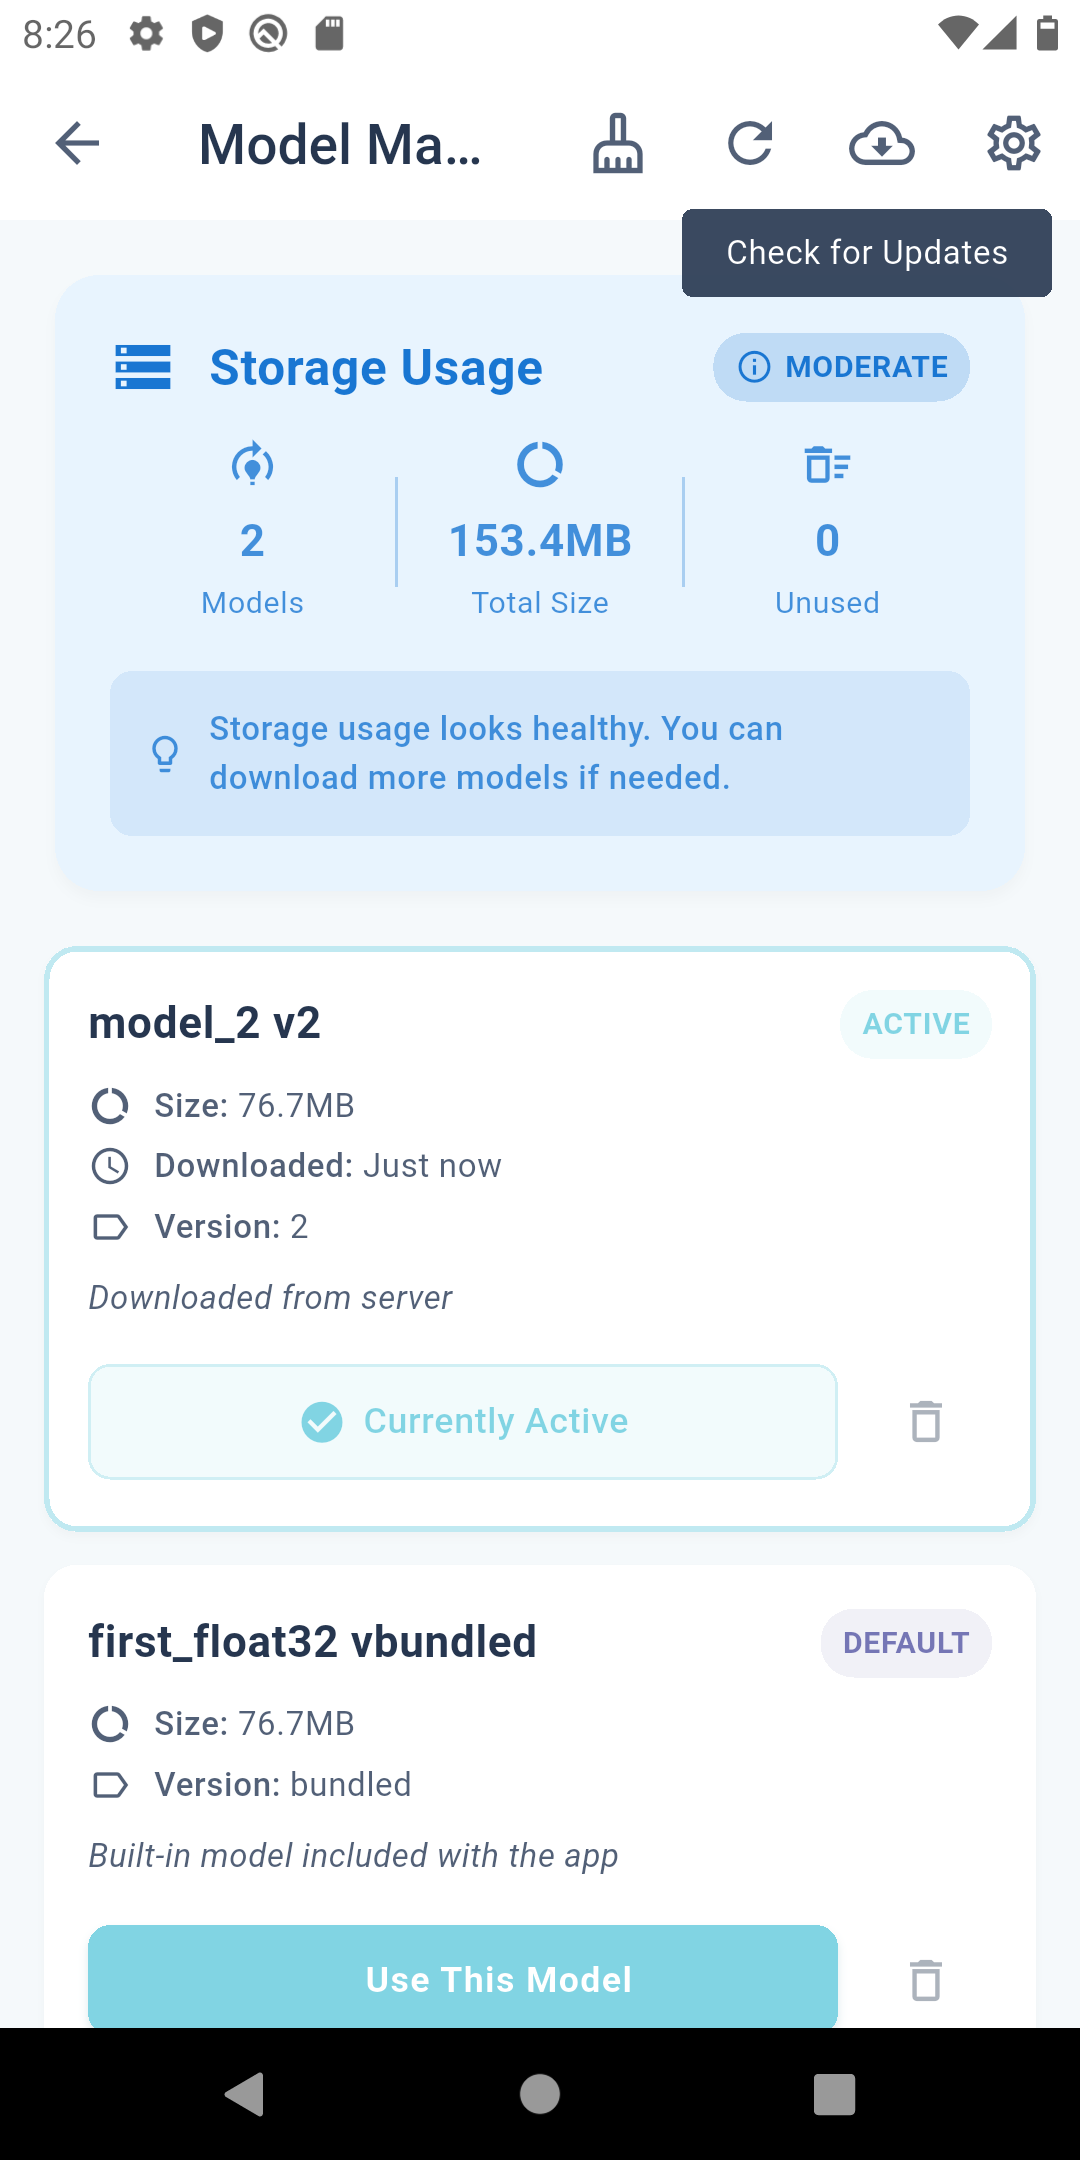
\includegraphics[height=0.5\textheight]{images/images/mobile_app/revision/CheckForUpdates.png}
        \caption{Model Update}
    \end{minipage}
    \hfill
    \begin{minipage}[b]{0.48\textwidth}
        \centering
        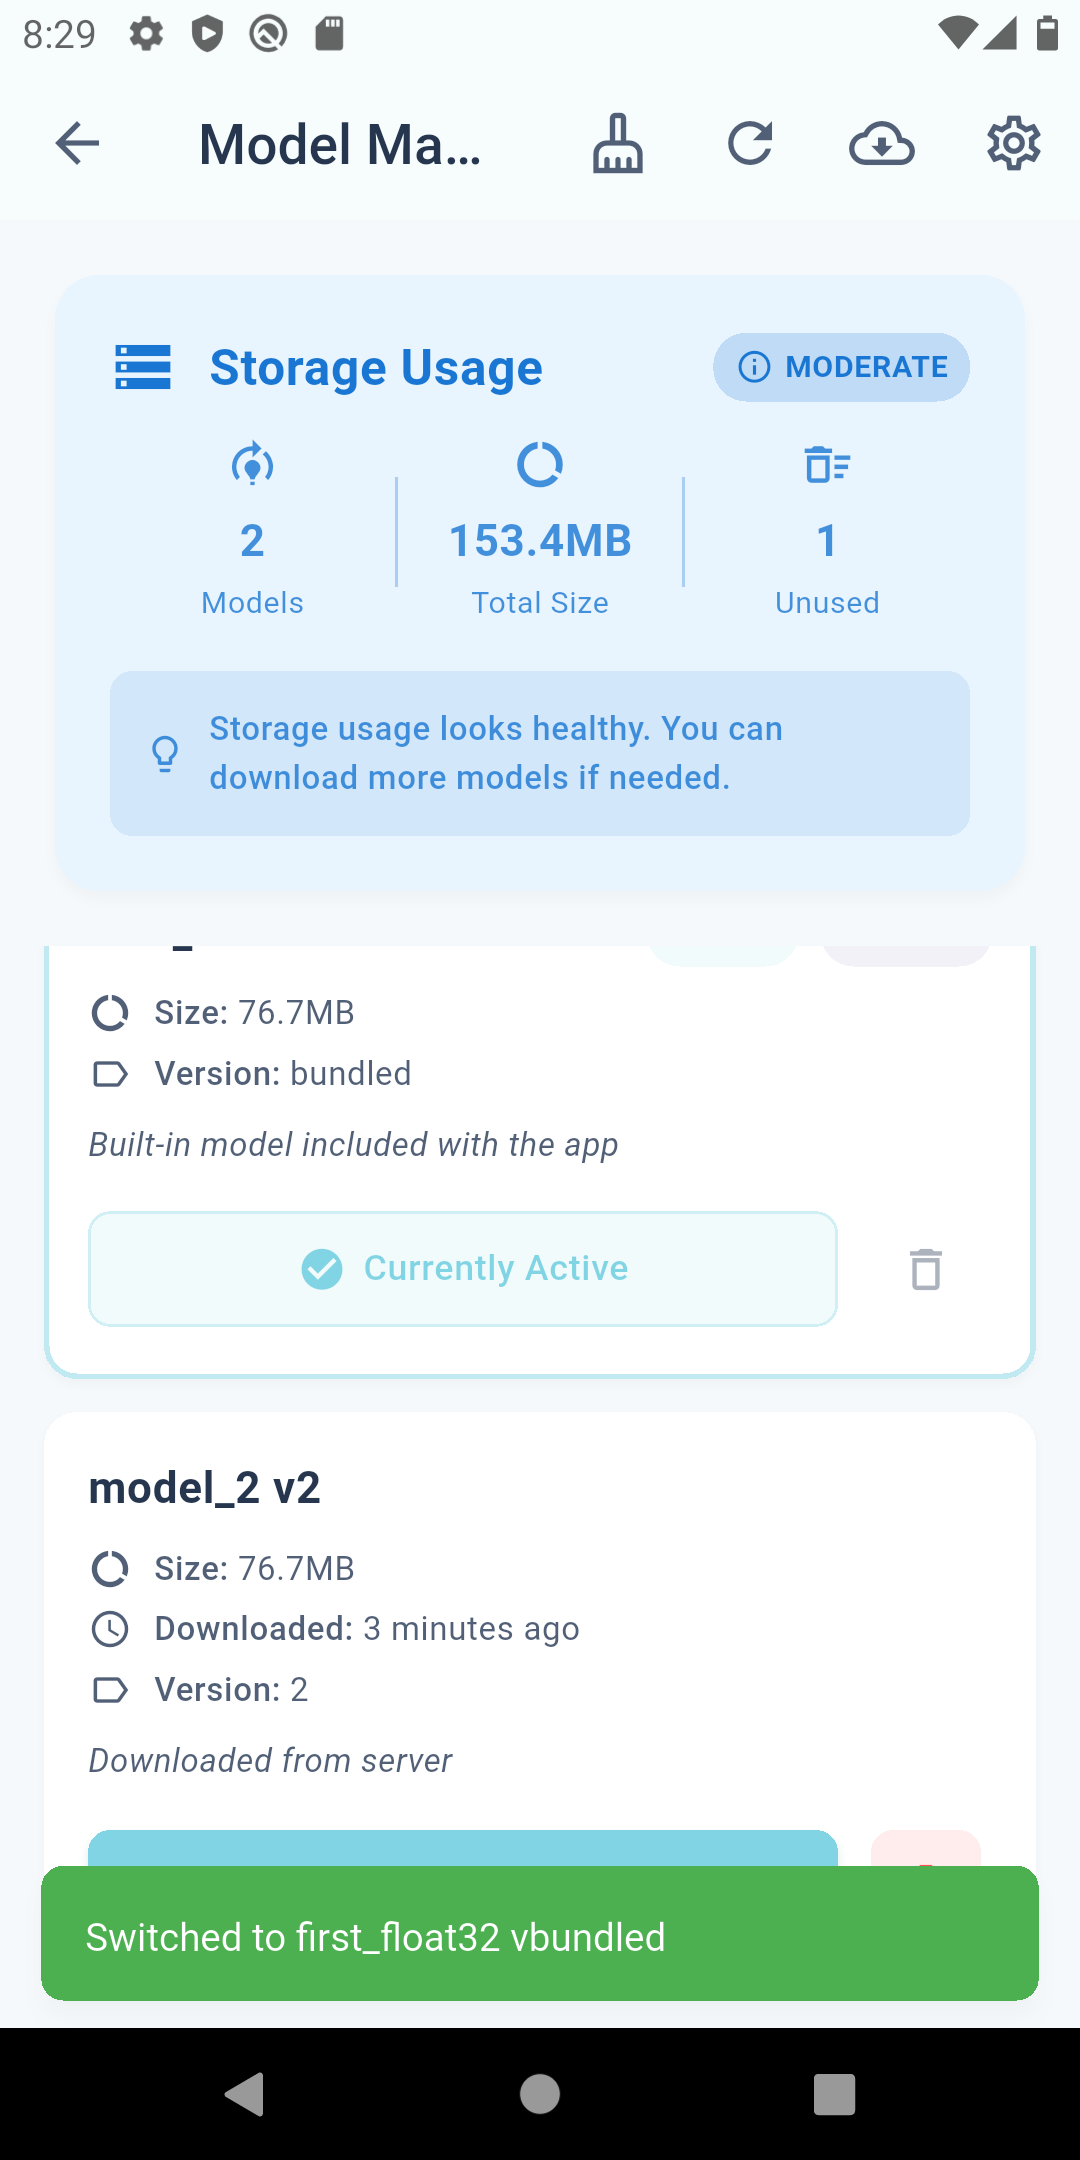
\includegraphics[height=0.5\textheight]{images/images/mobile_app/revision/SwitchingOfModel.png}
        \caption{Switch Model}
    \end{minipage}
    \end{figure}

\subsection{AI Model Management}
In the AI Model Management section of the User Profile, users can view and manage all available AI models within the application. This includes a detailed list of currently active models, the designated default model, and models that are unused or inactive. For each model, the system provides essential metadata such as version number, storage size, and operational status. Users can also check for available model updates to ensure optimal performance and accuracy.

An additional functionality within this section is the ability to switch between models based on the user’s preferences. This feature allows users to select an alternative model if they wish to prioritize certain performance characteristics, test new versions, or revert to a previous stable release. By offering model switching, the system promotes flexibility, adaptability, and continuous improvement in AI performance.
\newpage

 \begin{figure}[H]
       \begin{minipage}[b]{0.48\textwidth}
        \centering
        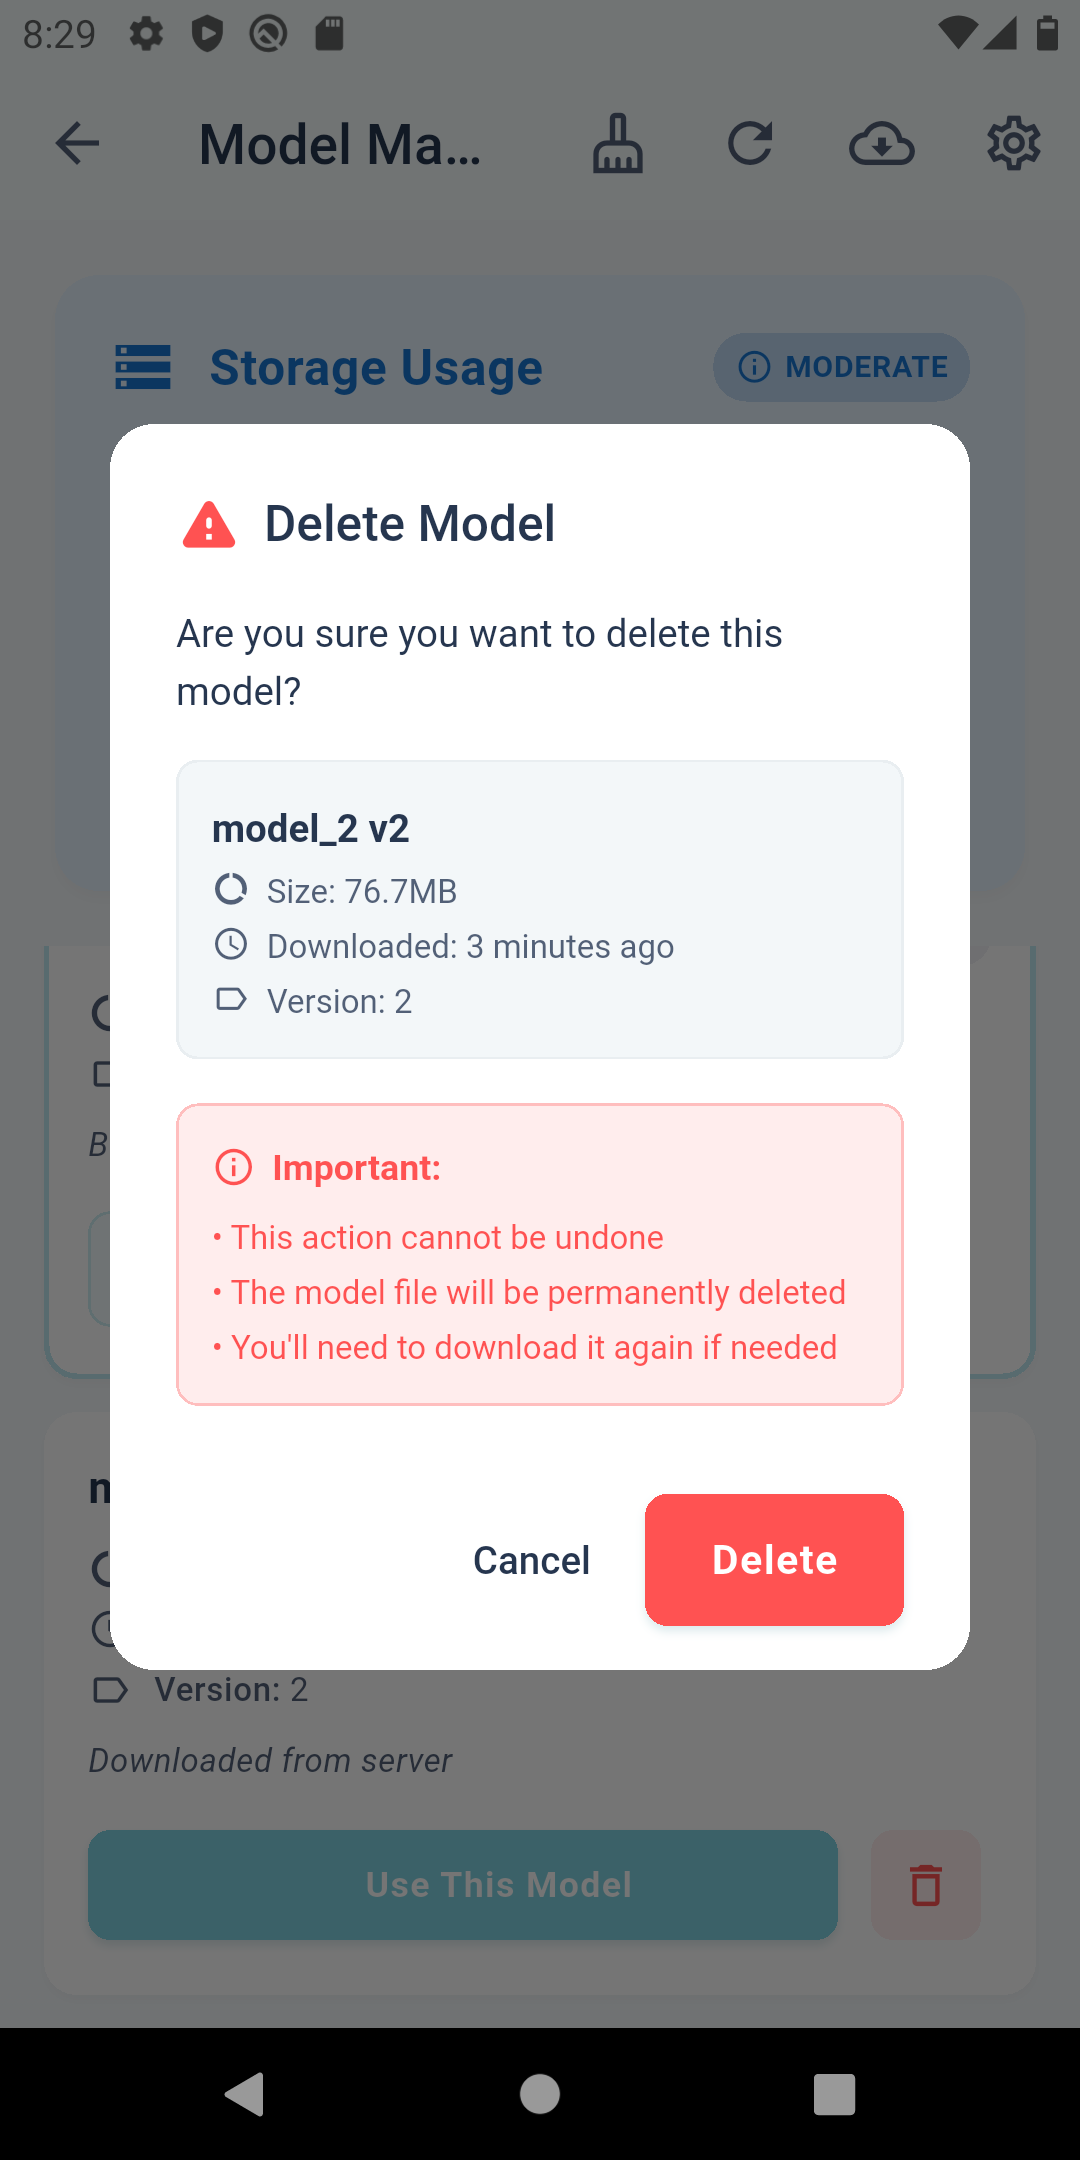
\includegraphics[height=0.6\textheight]{images/images/mobile_app/revision/DeleteModalDialog.png}
        \caption{Delete Model}
    \end{minipage}
    \hfill
    \begin{minipage}[b]{0.48\textwidth}
        \centering
        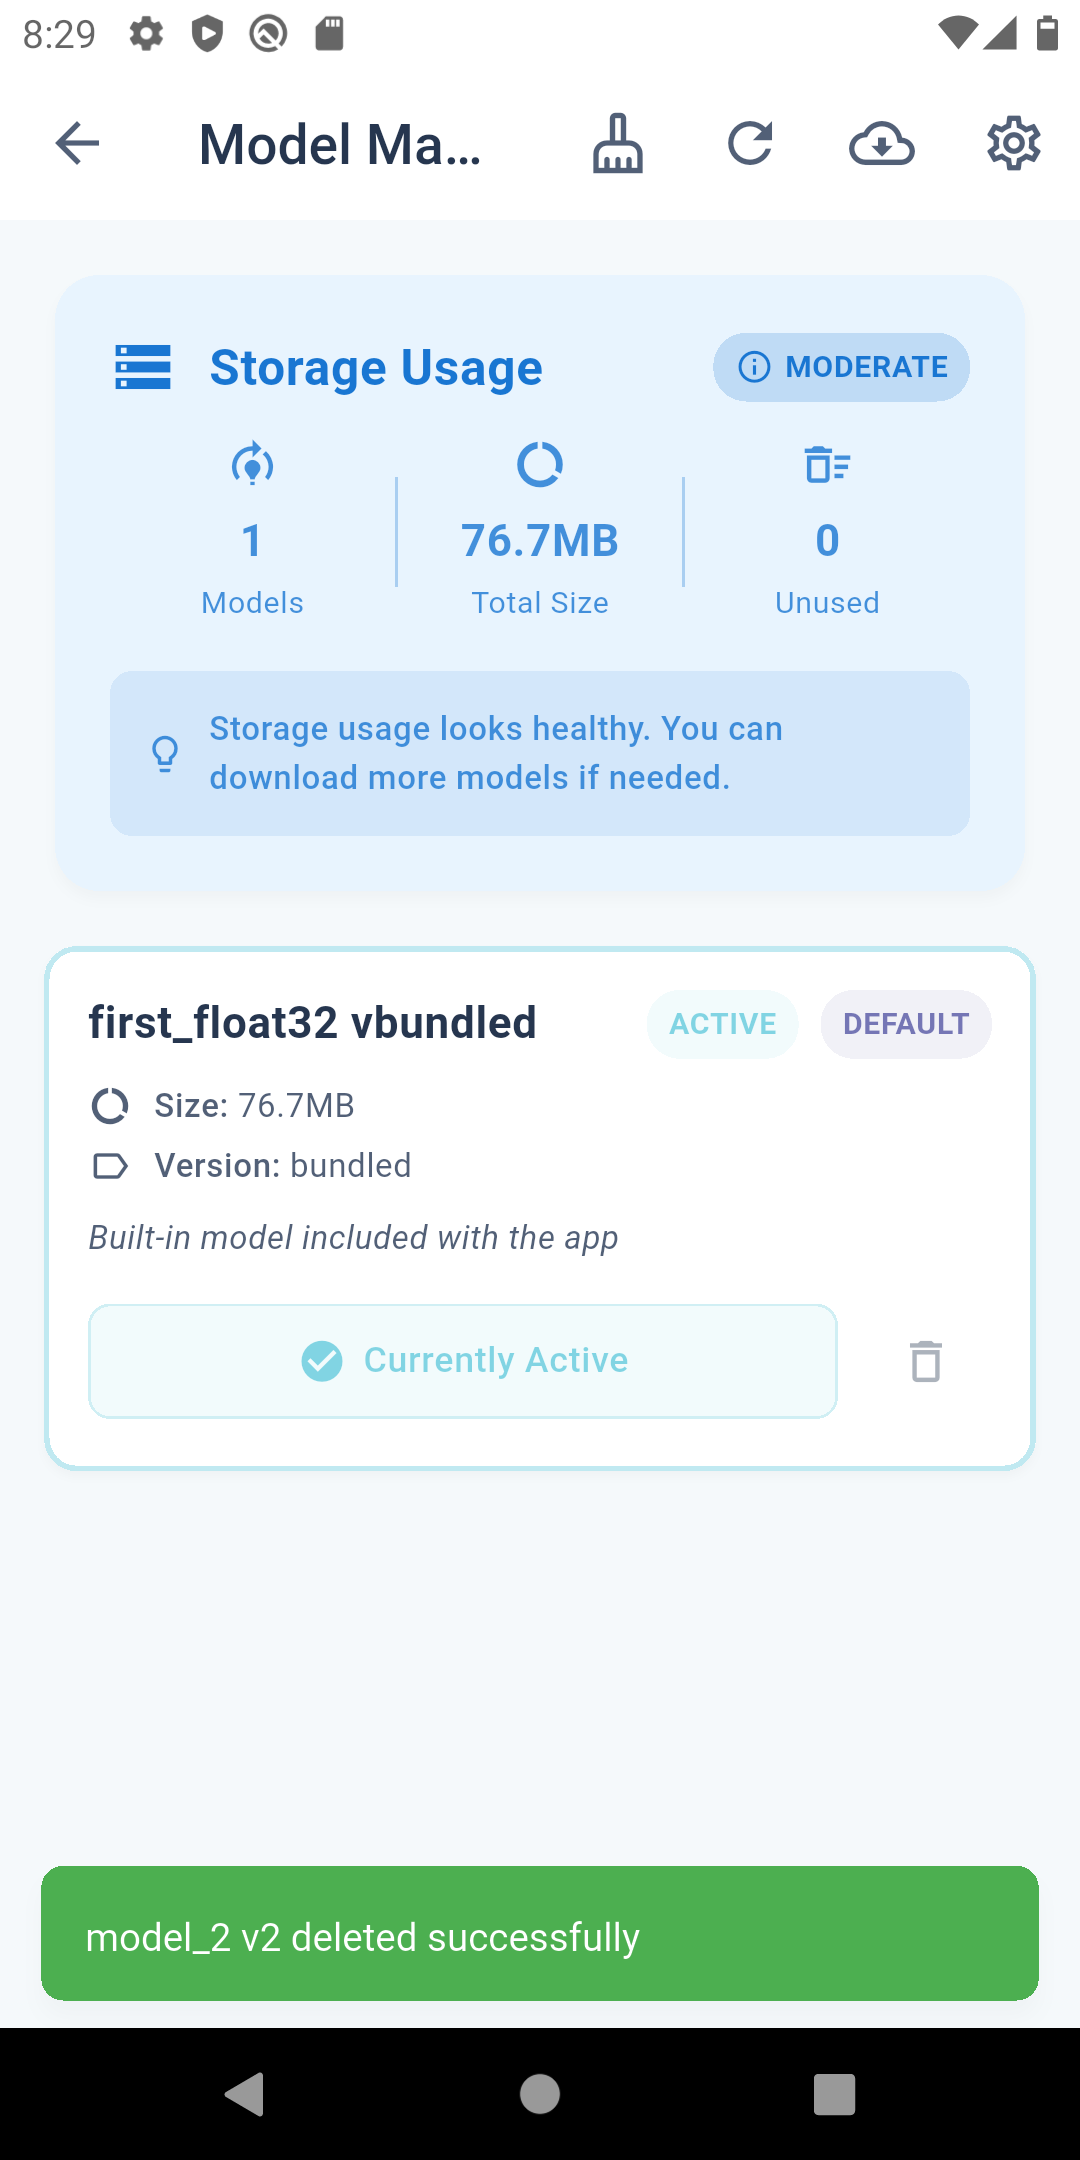
\includegraphics[height=0.6\textheight]{images/images/mobile_app/revision/SuccesfulyDeleteModel.png}
        \caption{Successful Model Deletion}
    \end{minipage}
    \end{figure}

\subsection{Model Deletion}
To delete a model, users can click the trash bin icon associated with the respective model. Once confirmed, this action is irreversible the model will be permanently removed from the application’s storage. If the deleted model is required in the future, it must be downloaded again from the model repository before it can be used. This feature ensures that users can manage storage efficiently while maintaining control over the AI models available in the system.
\newpage

\section{ClassiFish Mobile Application Web Admin Panel}

\begin{figure}[H]
    \makebox[\textwidth][c]{%
        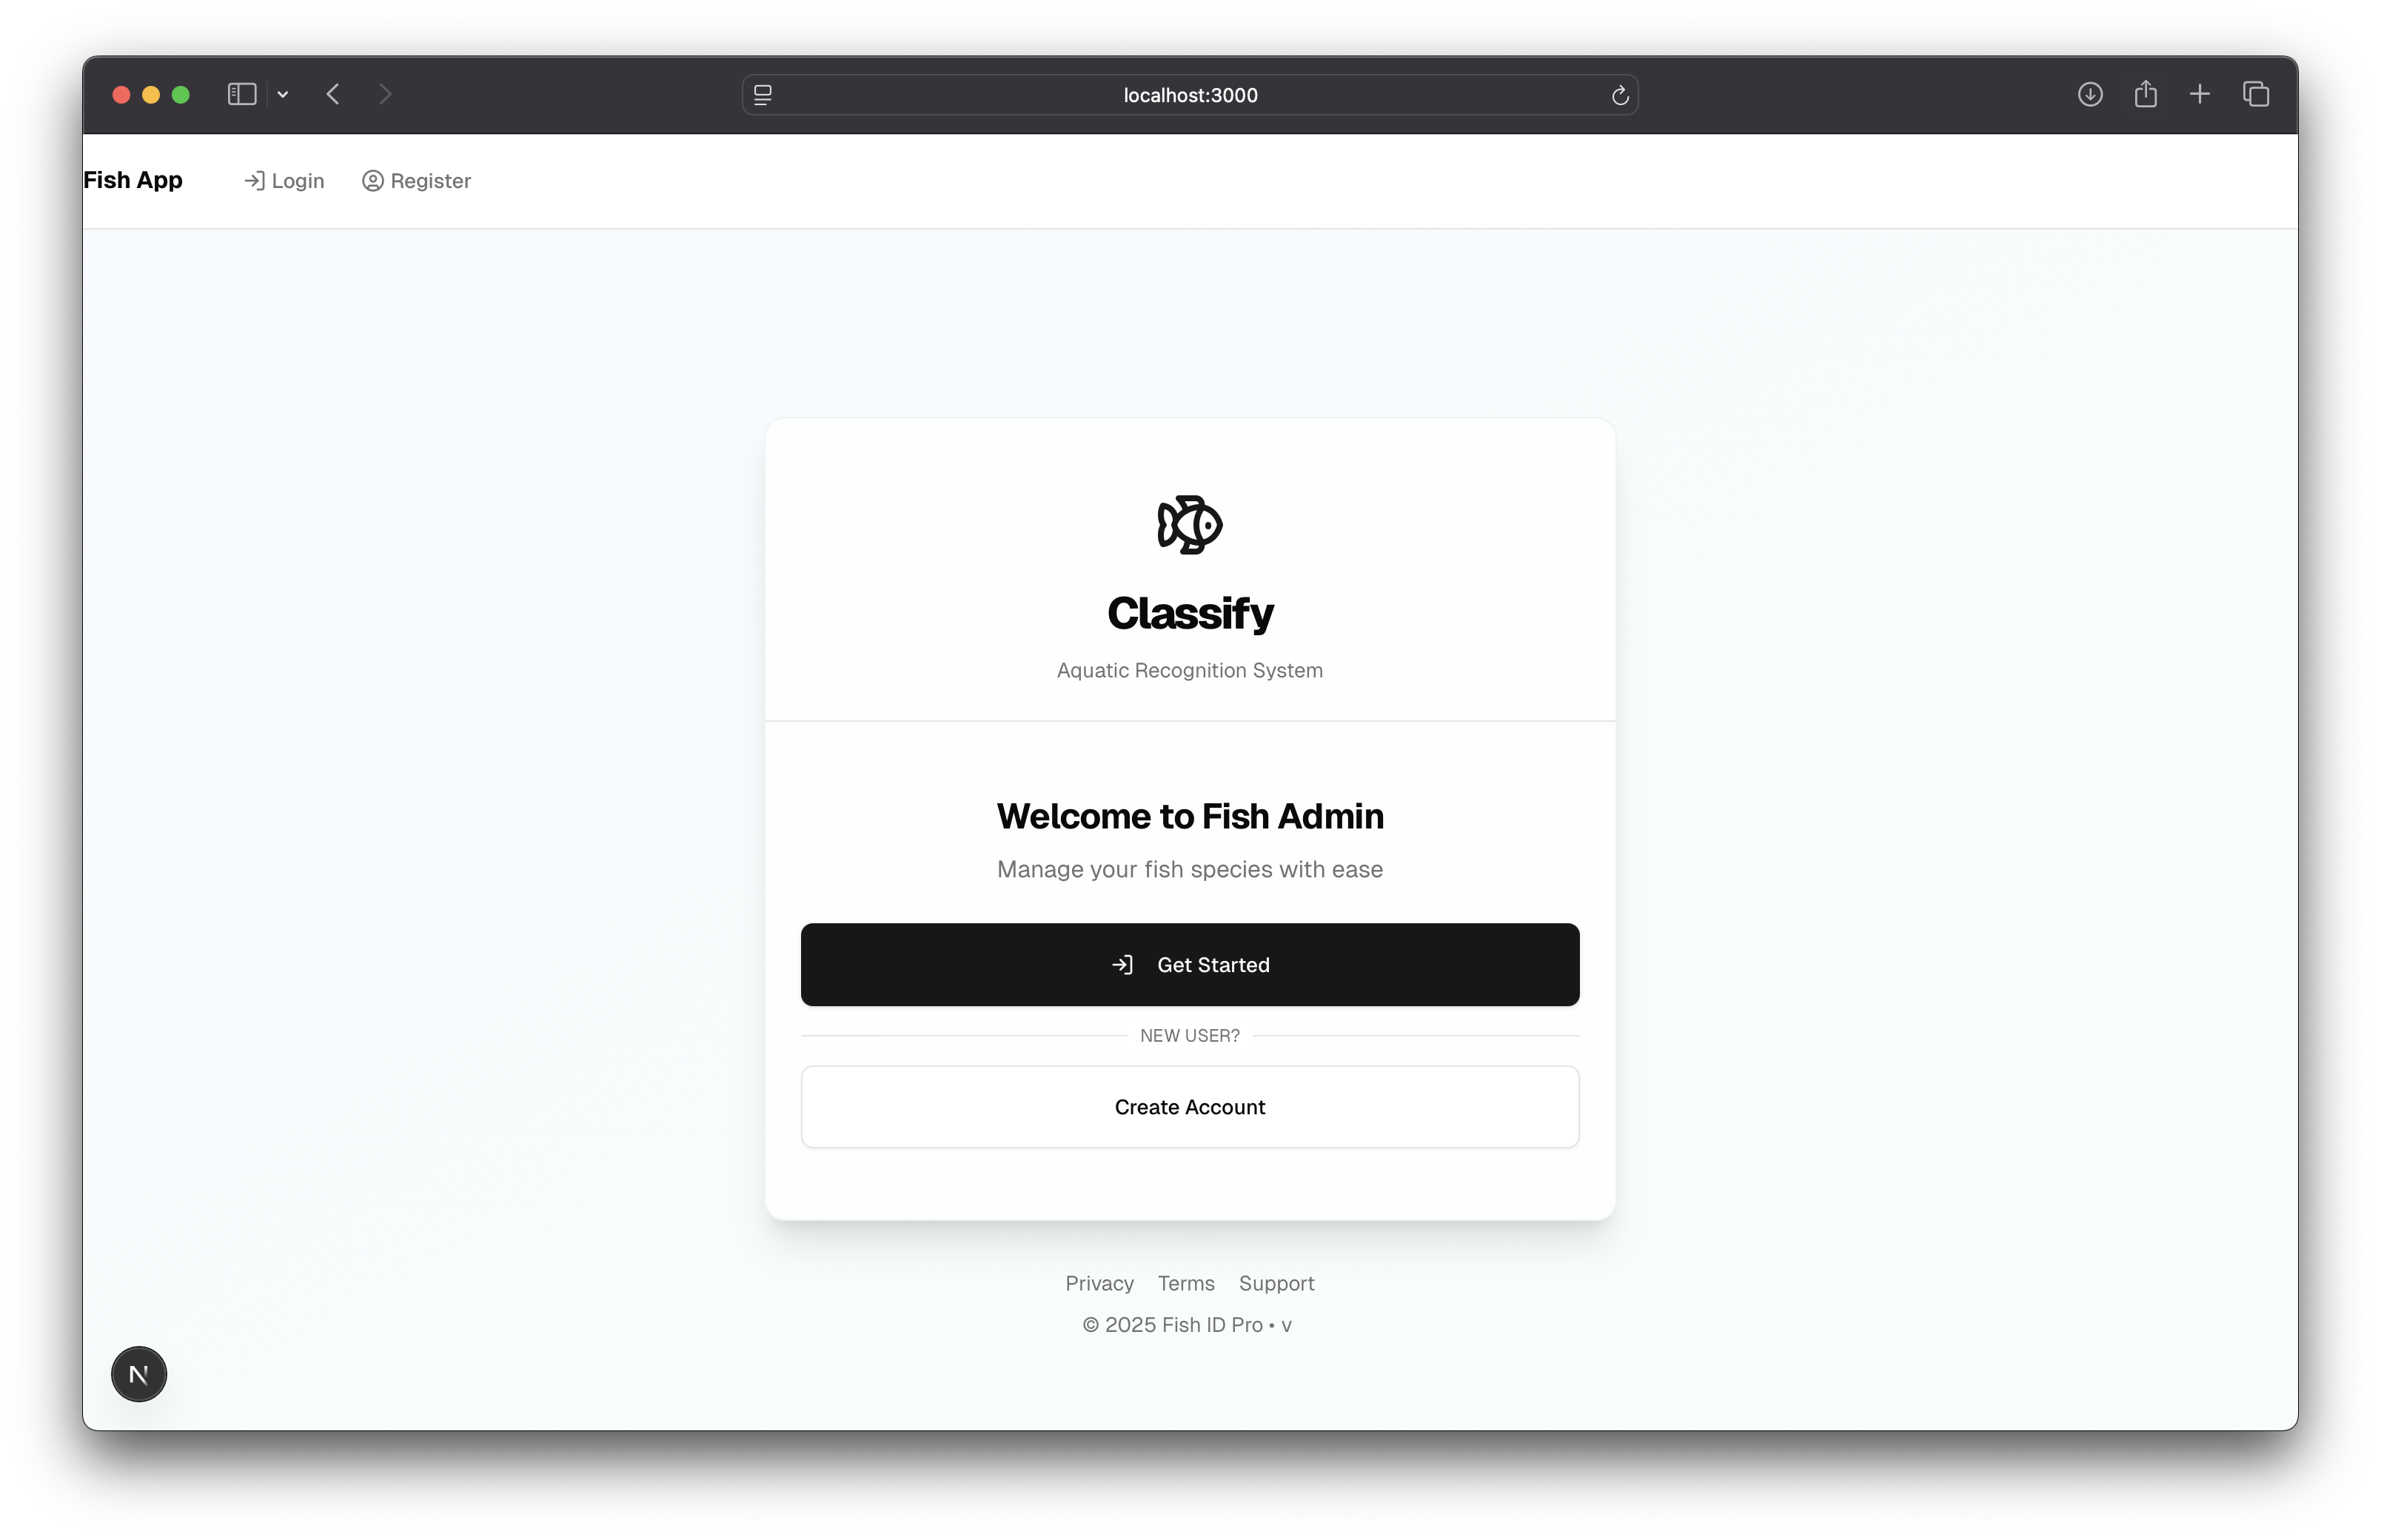
\includegraphics[width=1.2\textwidth]{images/images/WebApp/Landing_page.png}%
    }
    \caption{Admin Registration}
\end{figure}

\subsection{Admin Landing Page}
The admin landing page provides an option to get started by creating a new administrator account. The new administrator can register by completing the account creation process, which grants access to the admin panel for managing the ClassiFish mobile application.

\newpage
\begin{figure}[H]
    \makebox[\textwidth][c]{%
        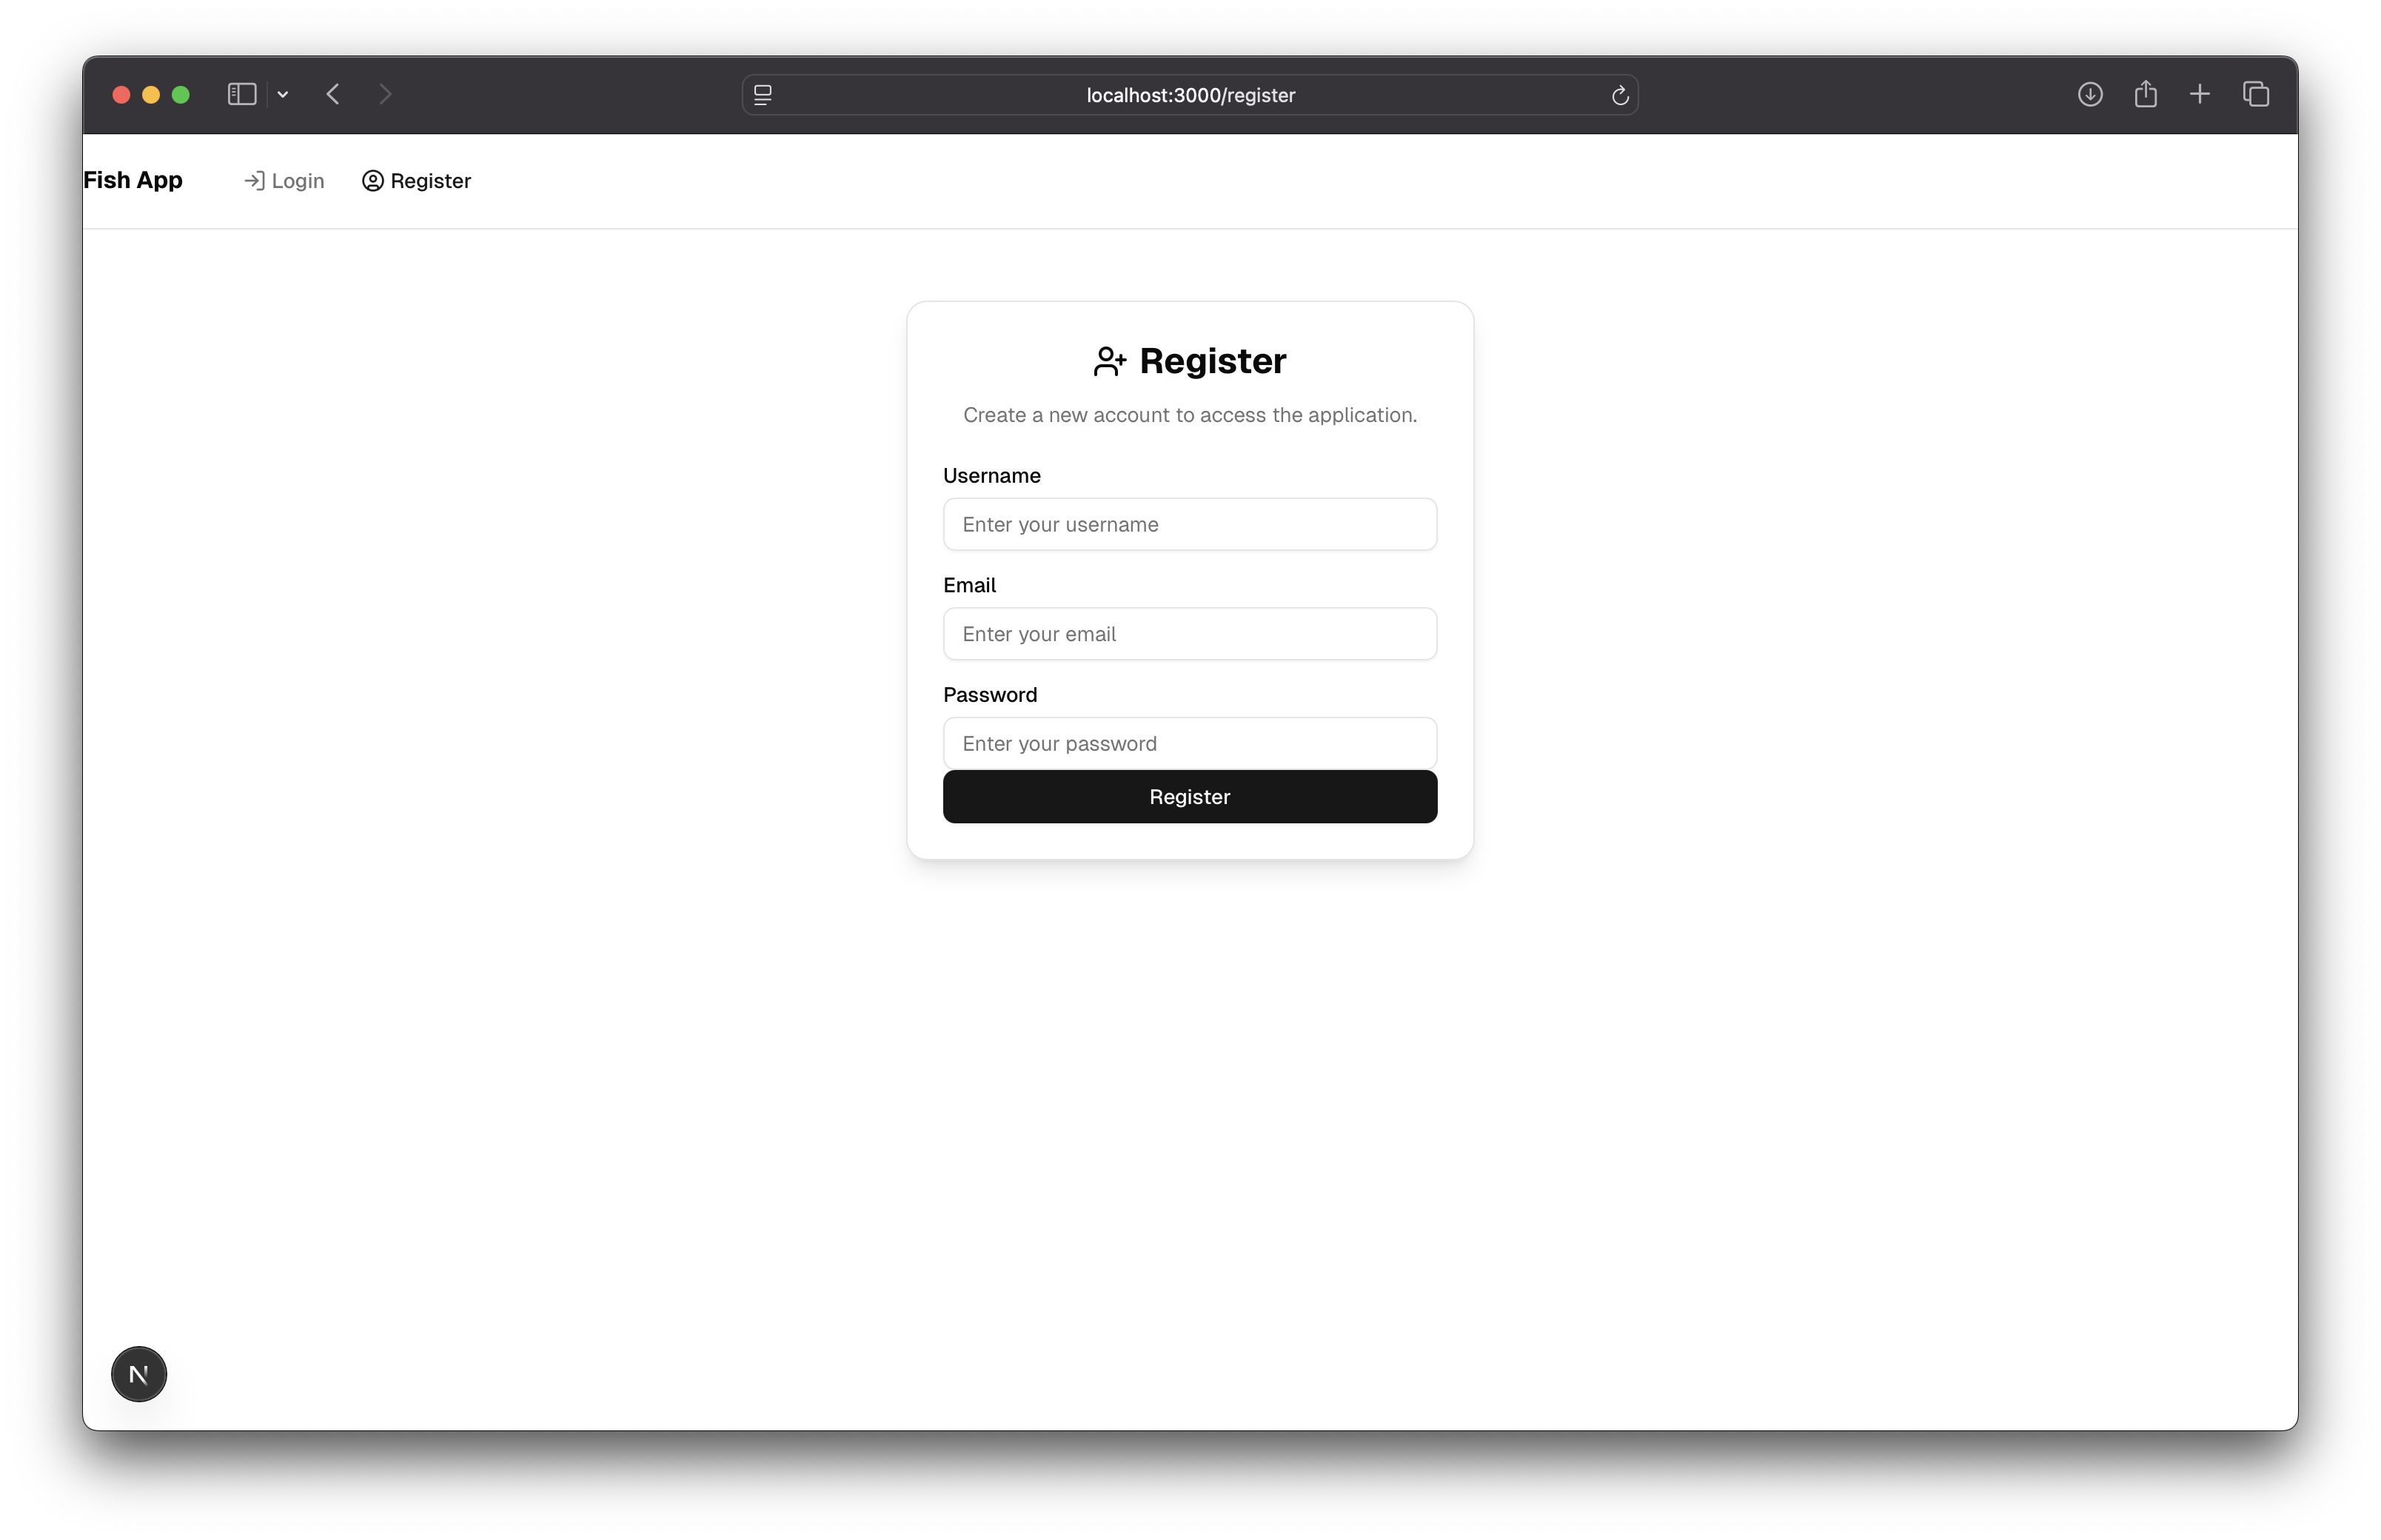
\includegraphics[width=1.2\textwidth]{images/images/WebApp/Admin_Register.png}%
    }
    \caption{Admin Register Page}
\end{figure}

\subsection{Admin Registration Page}
The admin registration page prompts the new administrator to enter essential information, including their full name, email address, and a secure password. These details are required to successfully create an administrator account and gain access to the admin panel for managing the ClassiFish mobile application.

\newpage
\begin{figure}[H]
    \makebox[\textwidth][c]{%
        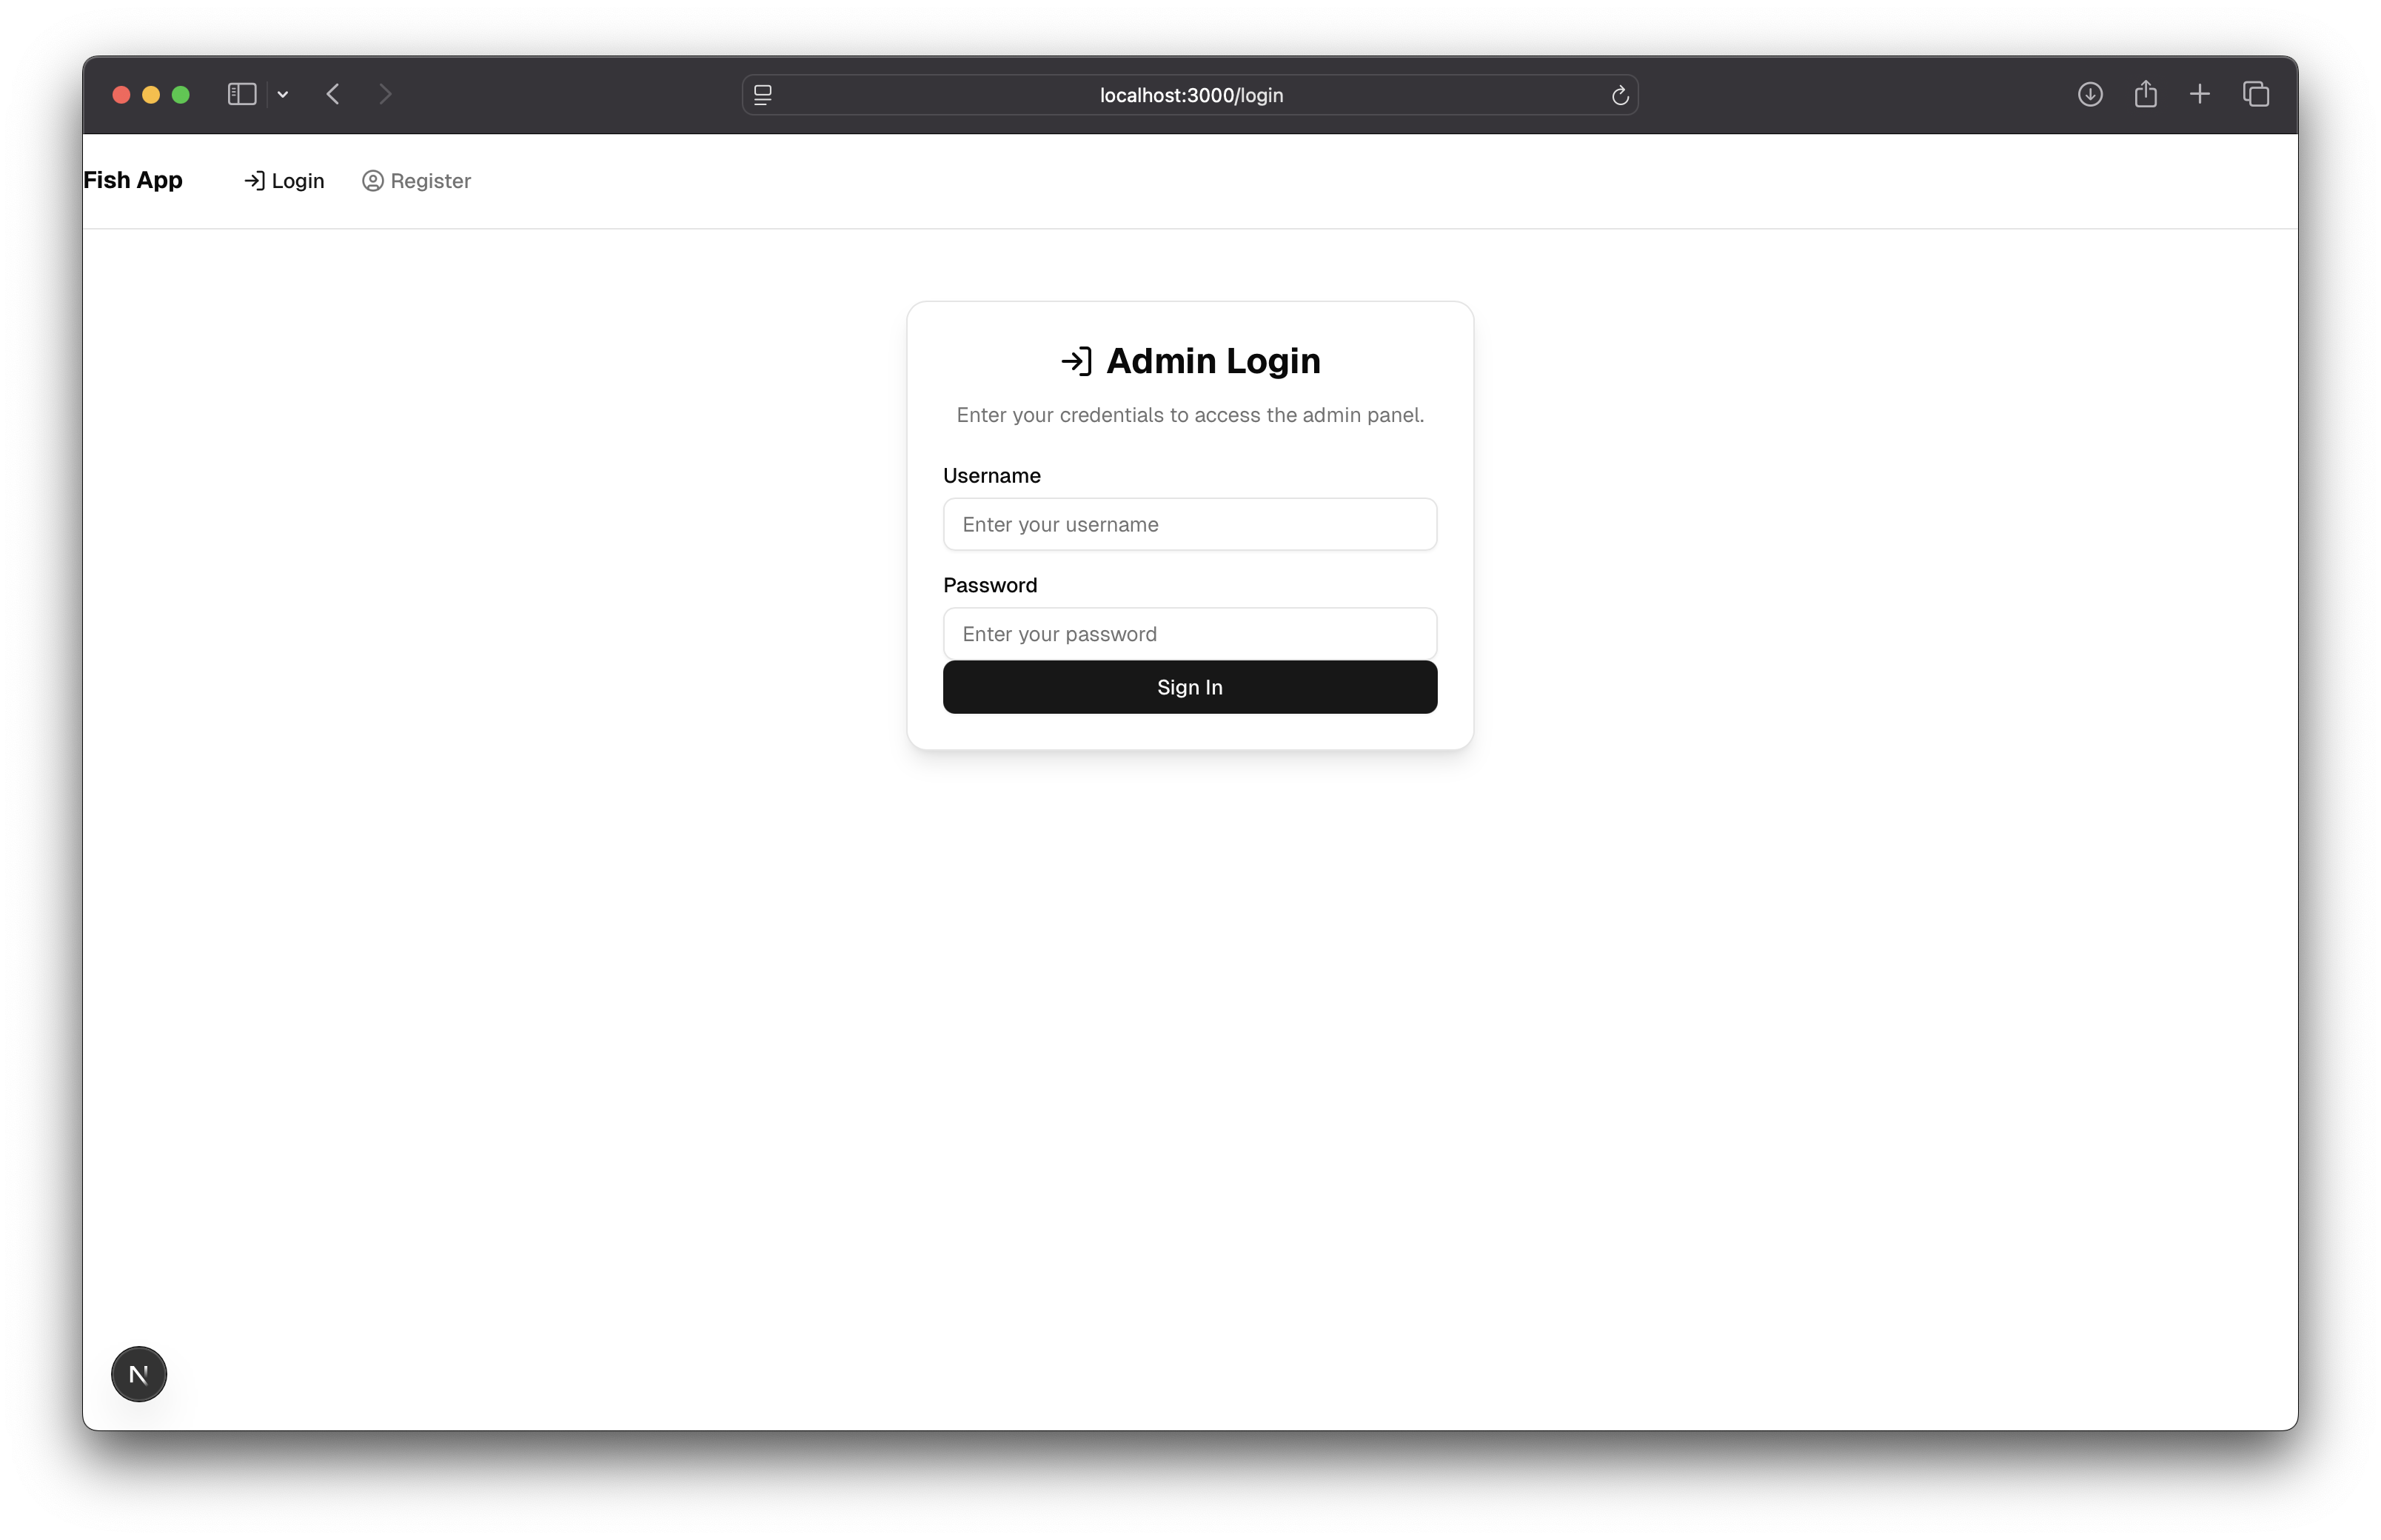
\includegraphics[width=1.2\textwidth]{images/images/WebApp/Admin_Login.png}%
    }
    \caption{Admin Login}
\end{figure}

\subsection{Admin Login Page}
The admin login page allows an administrator who already has an account to log in directly by entering their registered email address and password. Upon successful authentication, the administrator is granted access to the admin panel for managing the ClassiFish mobile application.
\newpage

\begin{figure}[H]
    \makebox[\textwidth][c]{%
        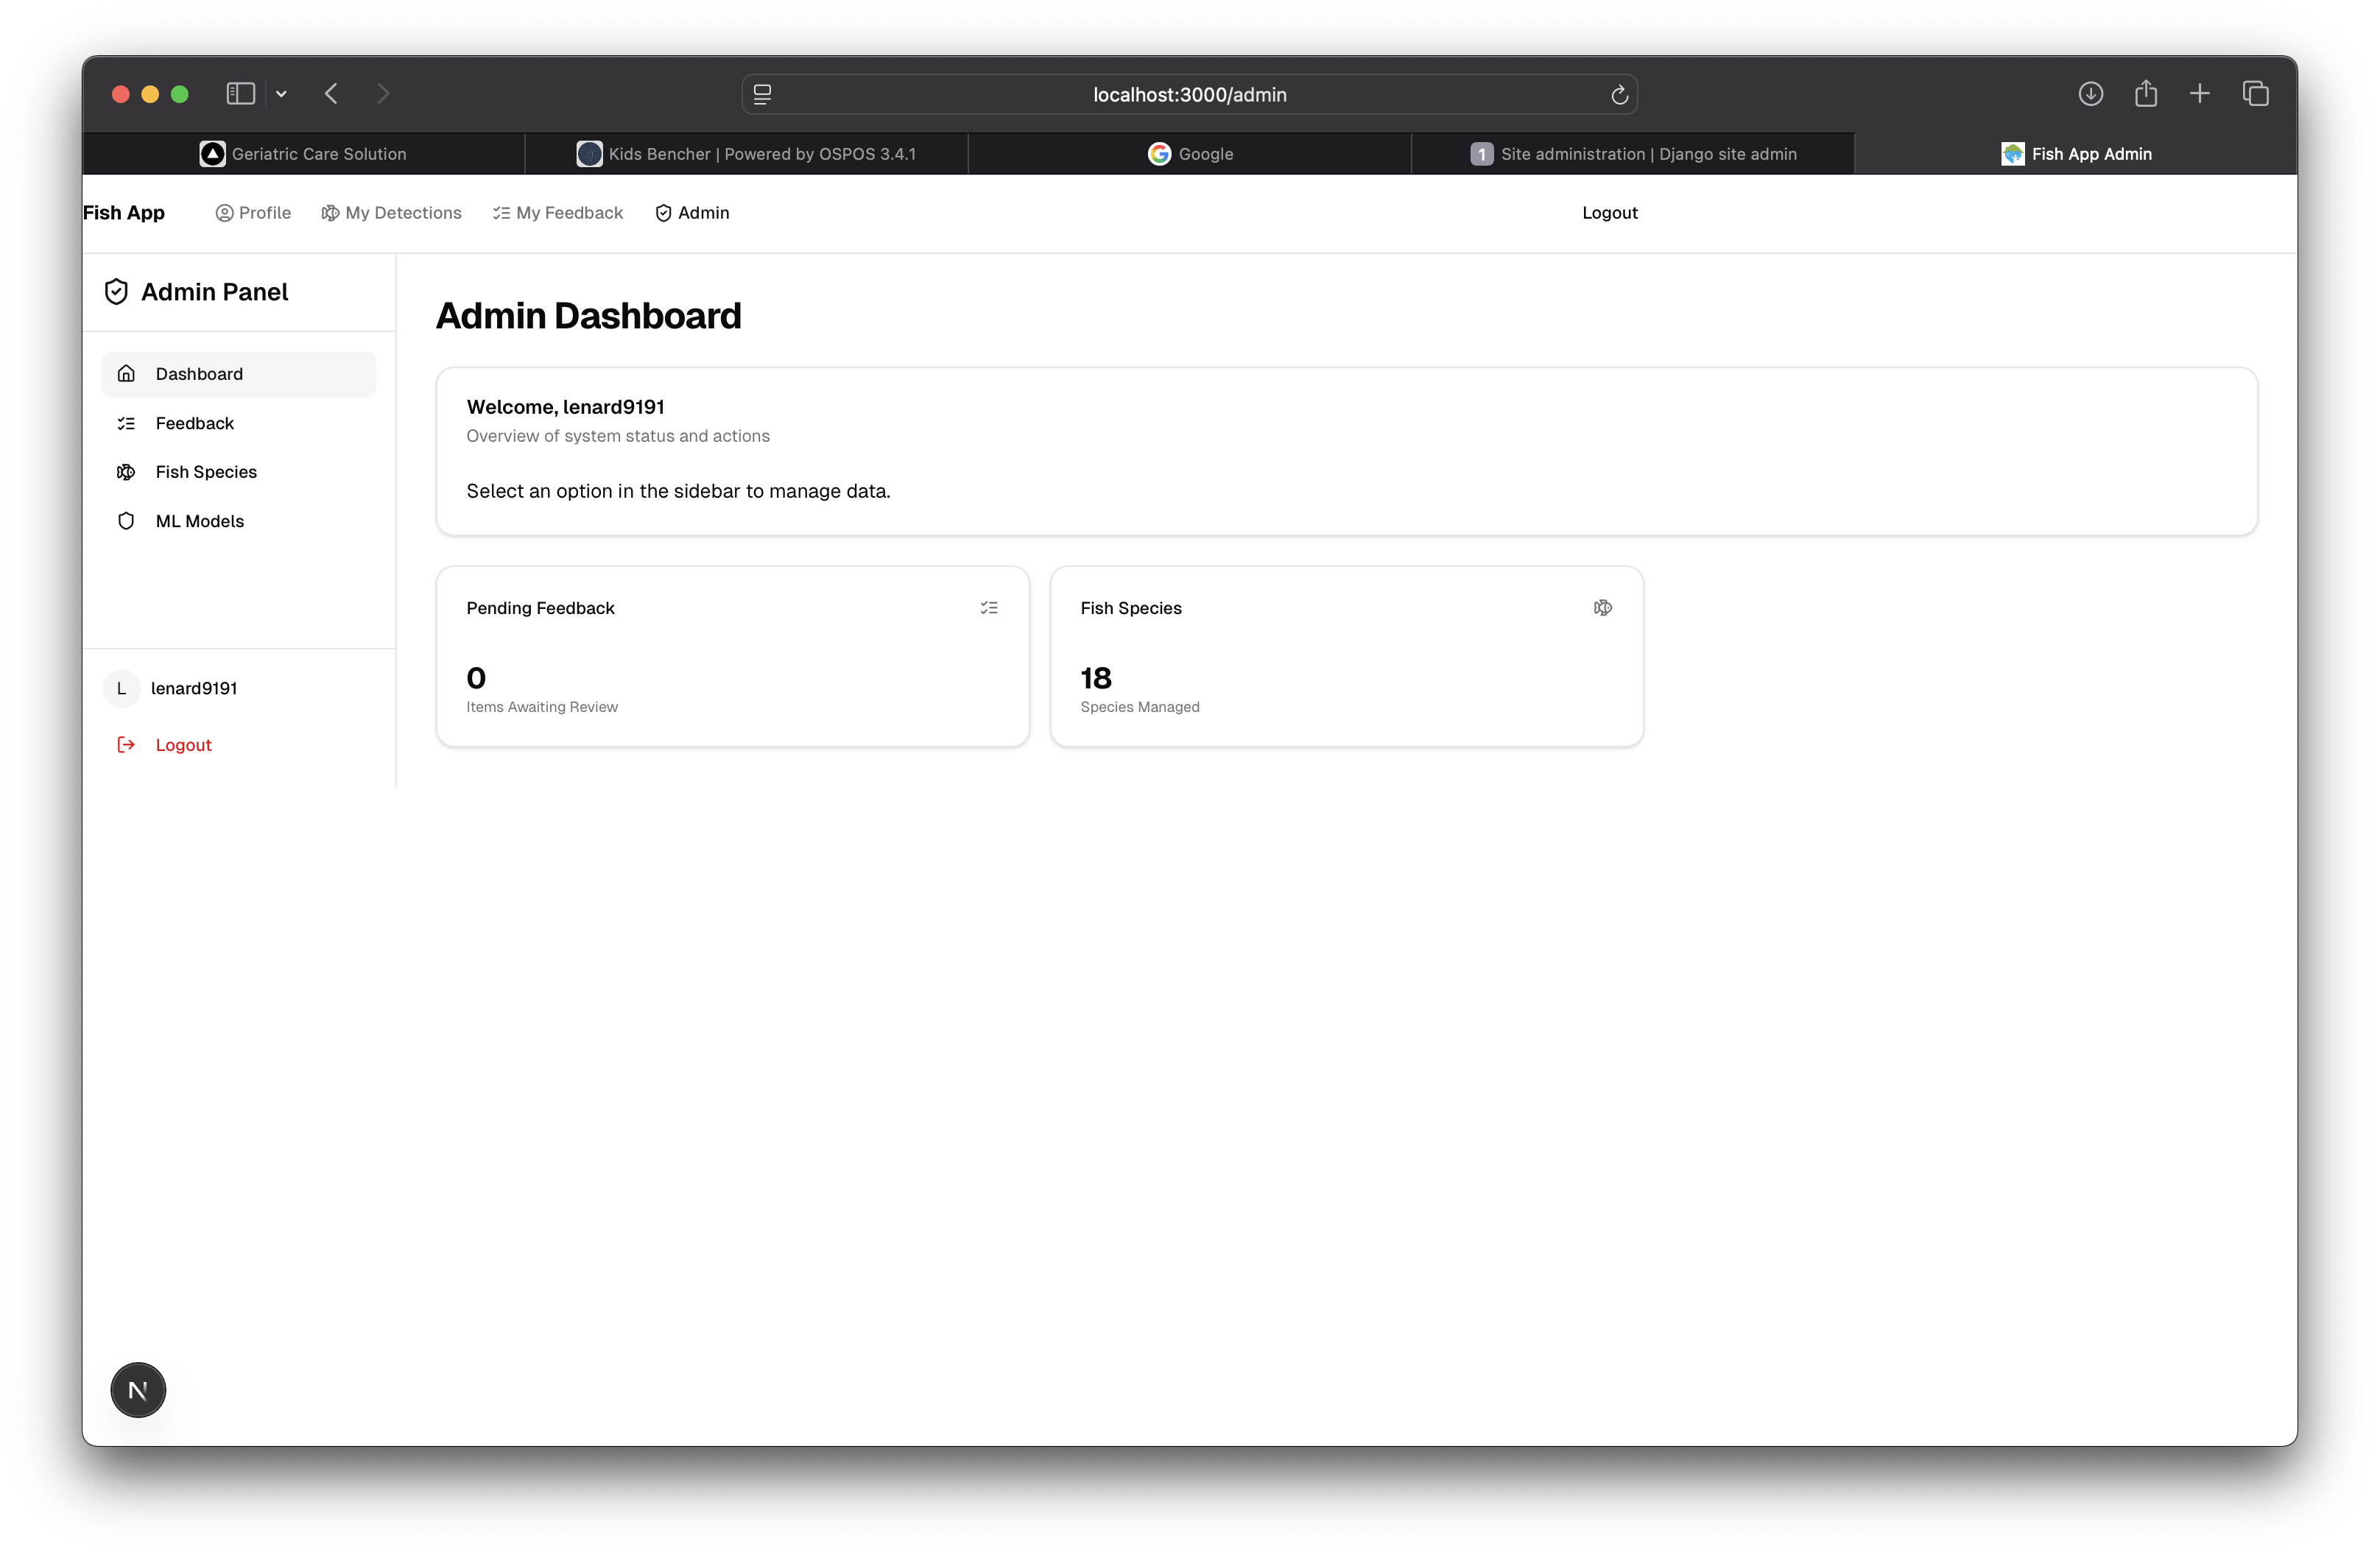
\includegraphics[width=1.2\textwidth]{images/images/mobile_app/revision/DashBoard.png}%
    }
    \caption{Admin Dashboard}
\end{figure}
\subsection{Admin Dashboard Page}
Upon successfully logging in, the administrator is directed to the admin dashboard, which presents an overview of the fish species and the pending feedback that requires review. In the sidebar navigation panel, the administrator can access and manage the Feedback Management section, the Fish Species module, and the Machine Learning Models module.
\newpage

\begin{figure}[H]
    \makebox[\textwidth][c]{%
        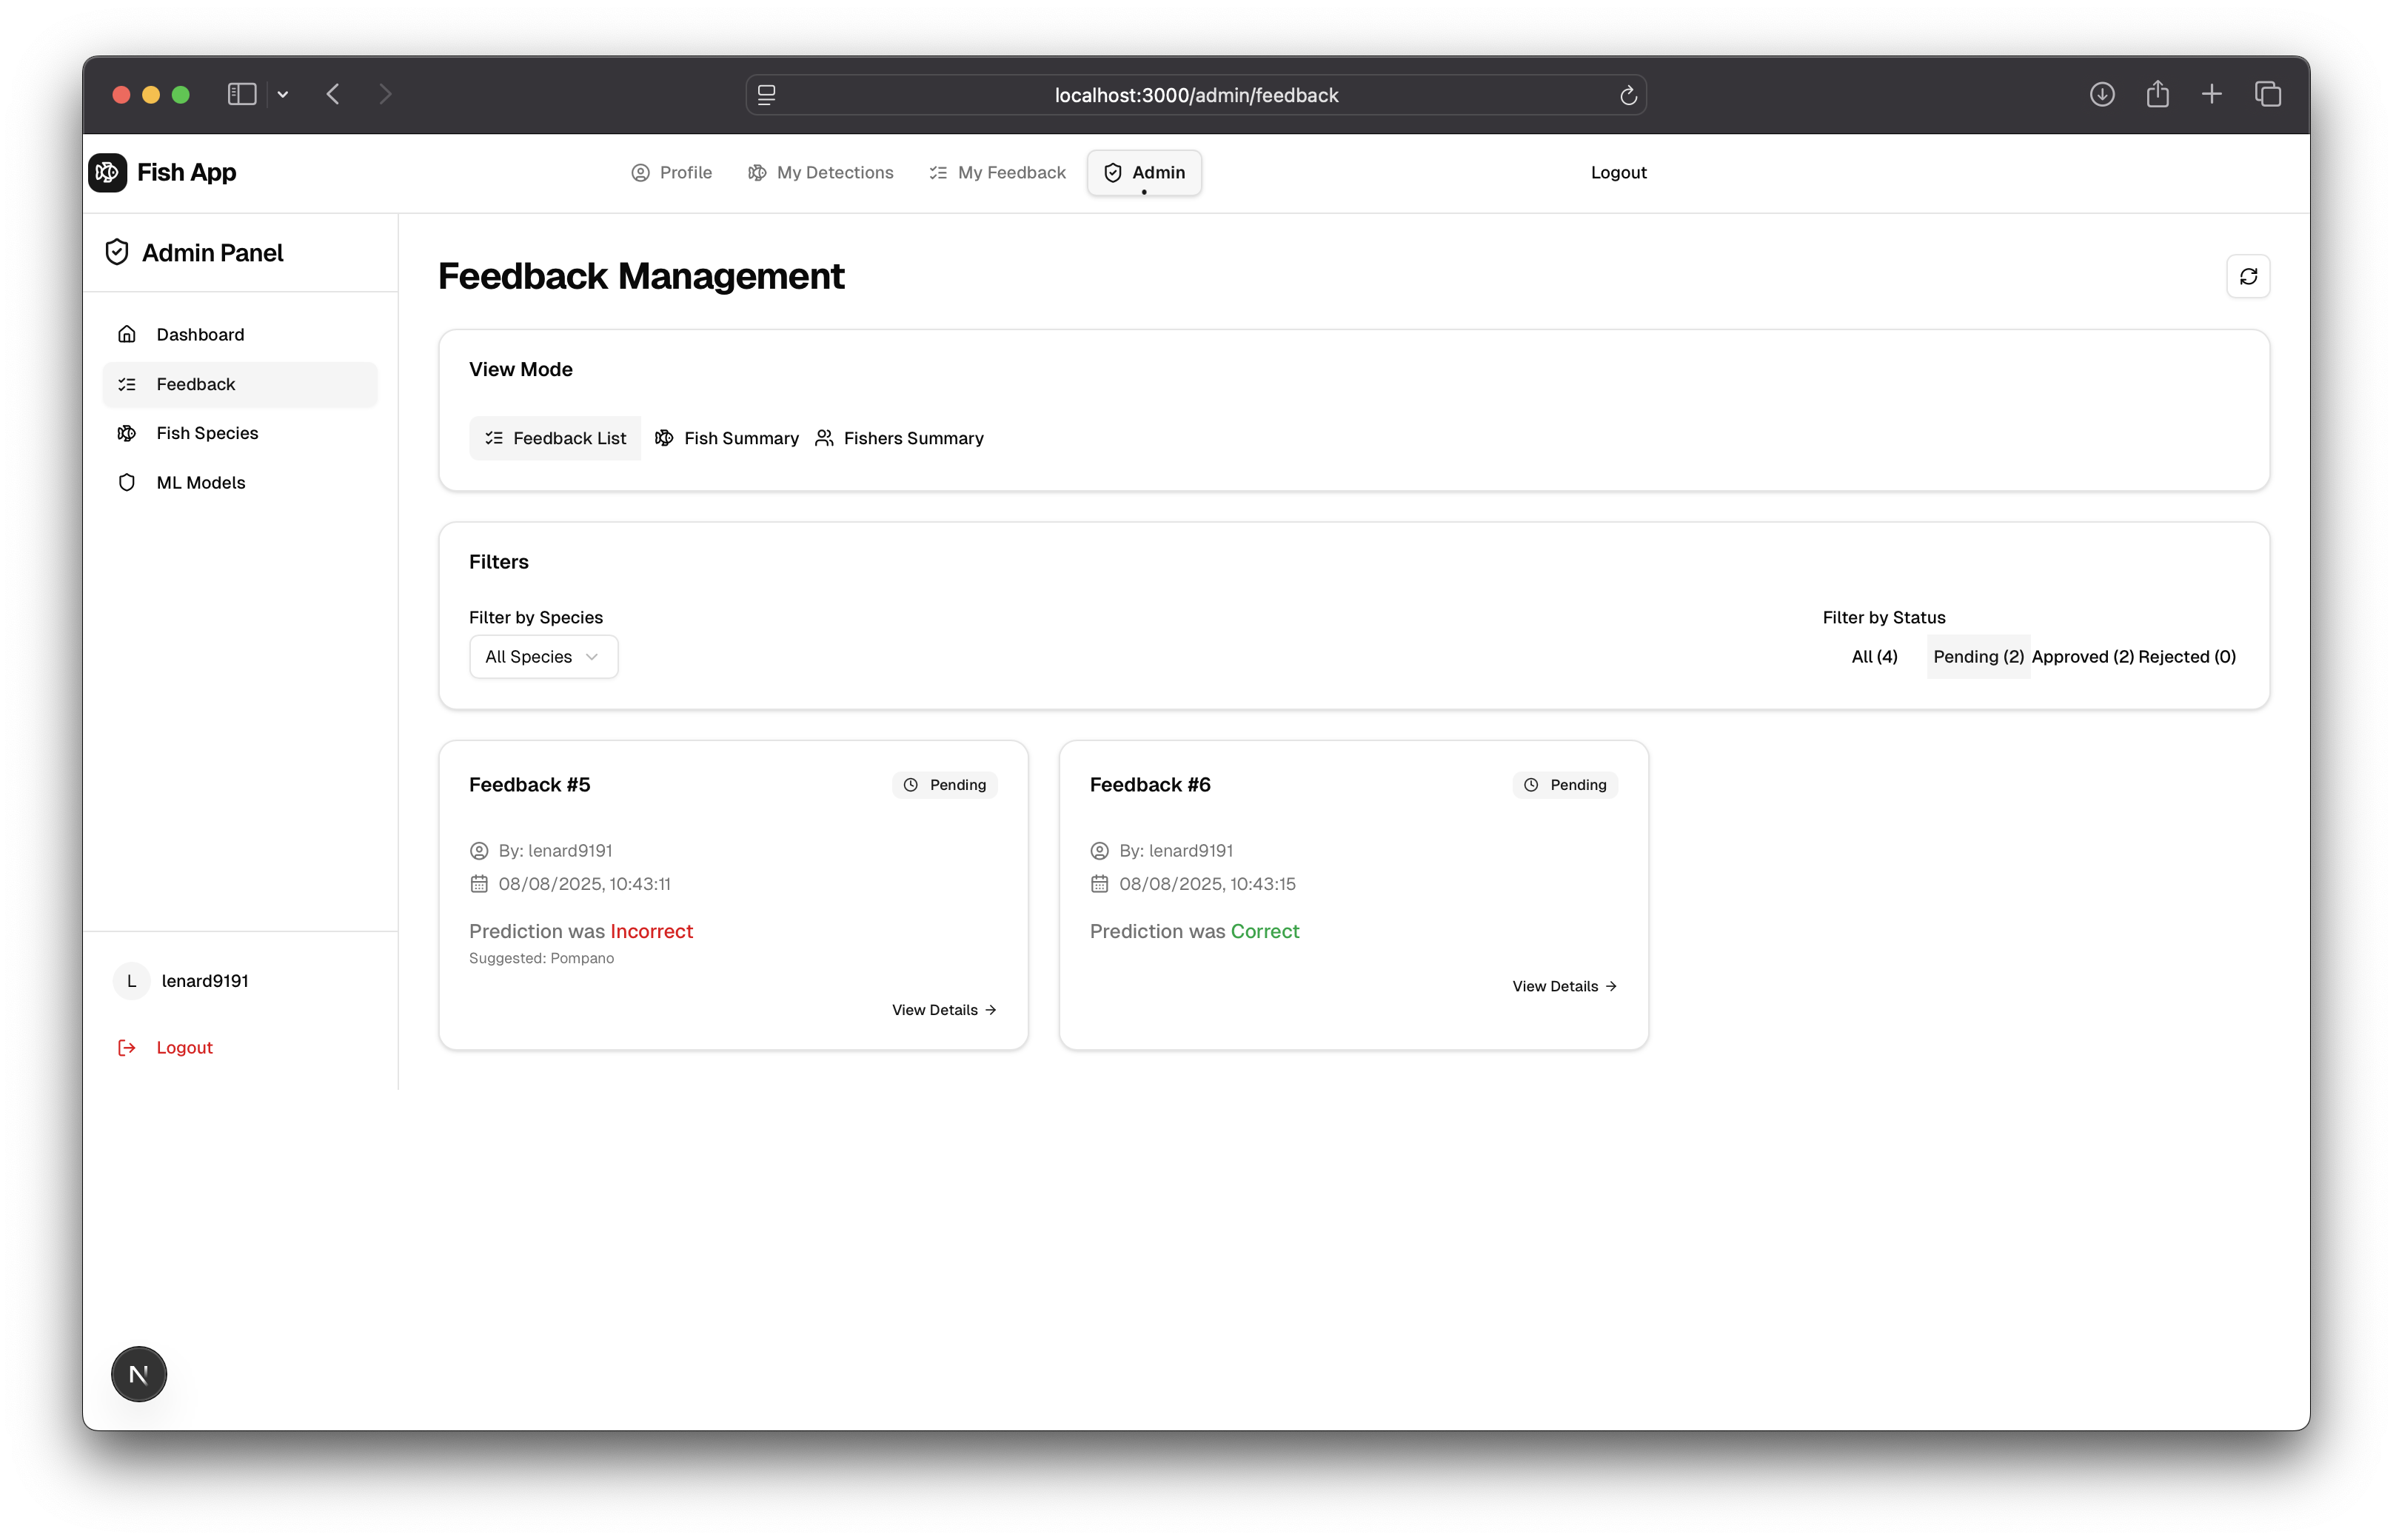
\includegraphics[width=1.2\textwidth]{images/images/mobile_app/revision/FeedbackPageWhereWeSelectAfeedback.png}%
    }
    \caption{Feedback Management}
\end{figure}

\subsection{Feedback Management Page}
The Feedback Management section serves as the administrative interface for reviewing incorrect user feedback submitted through the mobile application. This section displays a comprehensive list of feedback entries, including the username, the exact date and time of submission, and the current status of each entry. Feedback items can be filtered according to the identified fish species or by their review status, which may include All, Pending, Approved, or Rejected. 
\newpage

\begin{figure}[H]
    \makebox[\textwidth][c]{%
        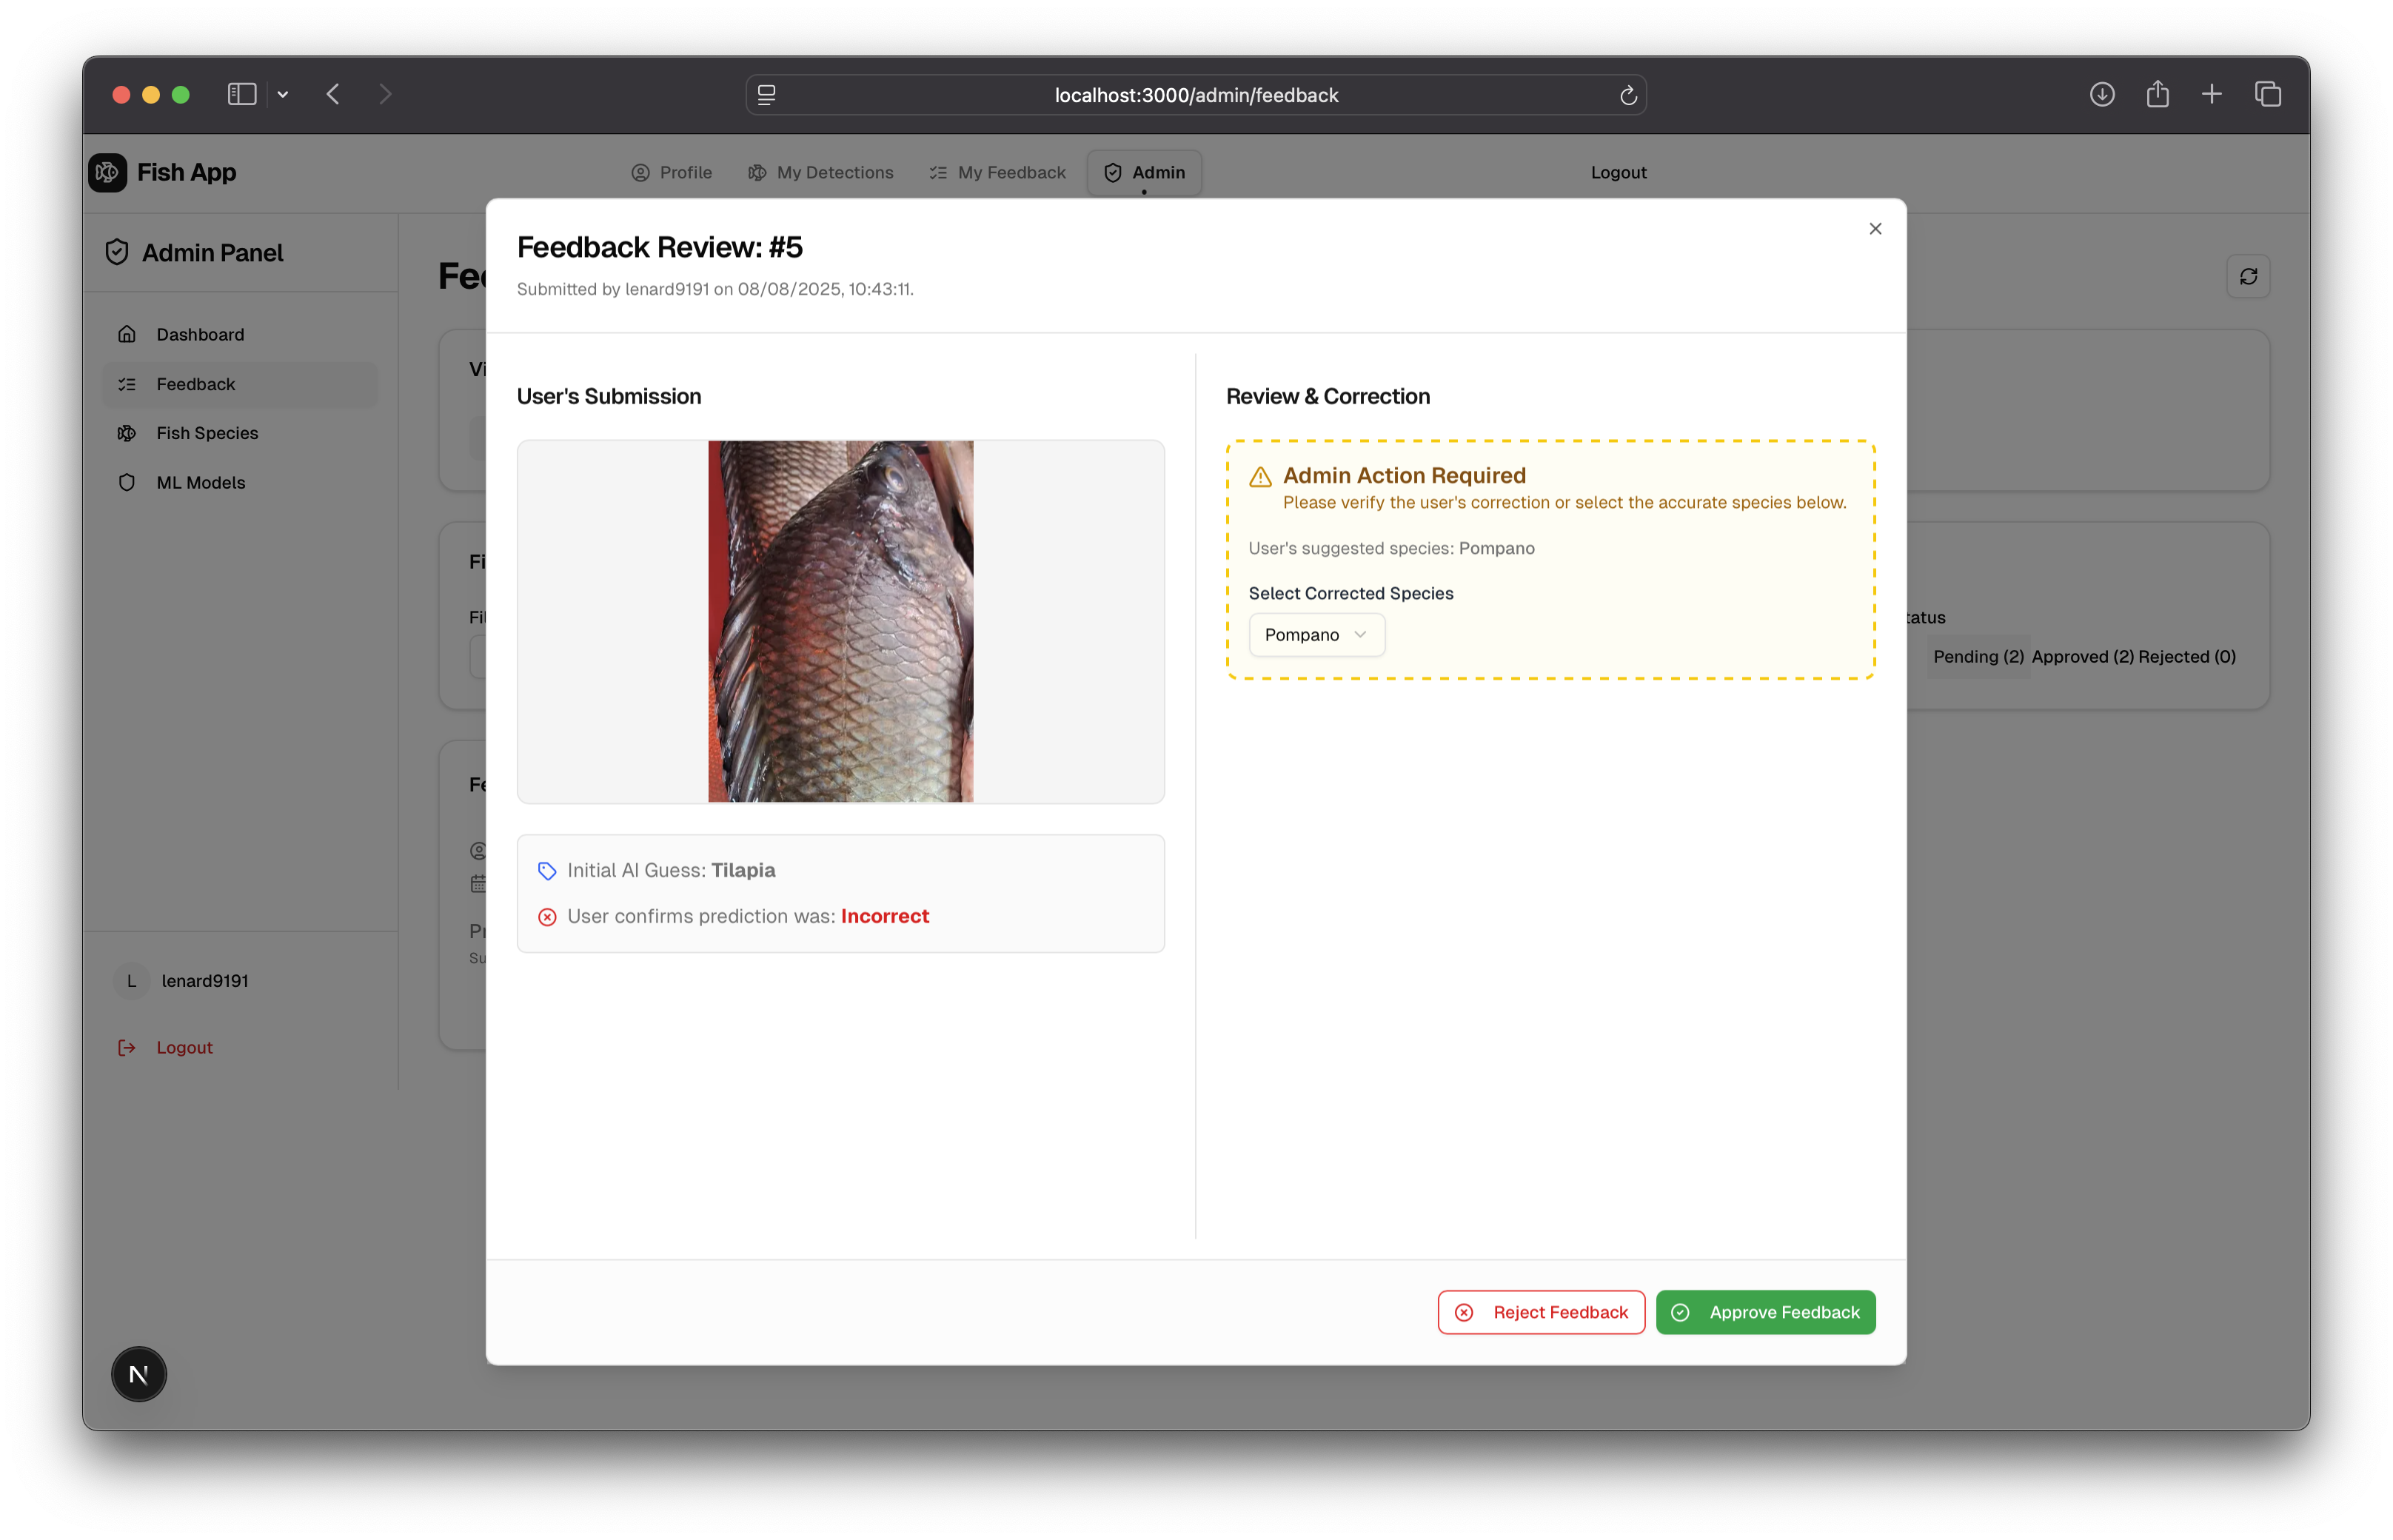
\includegraphics[width=1.2\textwidth]{images/images/mobile_app/revision/FeedbackDetails.png}%
    }
    \caption{Incorrect Feedback Details}
\end{figure}

\subsection{Incorrect Detection Feedback Review}
In the admin panel, all incorrect detection feedback submitted from the ClassiFish mobile application is received for evaluation. When a user identifies a specific detected bounding box that has been selected from among multiple detected boxes in an image as incorrect, they can mark it accordingly and select the correct fish species from the provided list. This feedback is then transmitted to the admin panel for review.

The administrator acts as a reviewer and is responsible for verifying whether the user-provided correction is accurate. The administrator must base their decision on credible references such as academic journals, scientific publications, and official fisheries websites. These sources help confirm the accuracy of fish species identification.

Based on the review, the administrator can either approve the correction, confirming that the user's feedback is valid, or reject it if the correction is deemed inaccurate. Approved feedback is stored in a dedicated feedback threshold repository, which serves as a reference dataset for future model retraining. This process enhances the detection efficiency of the ClassiFish application by incorporating verified corrections into the training data used for model updates.
\begin{figure}[H]
    \makebox[\textwidth][c]{%
        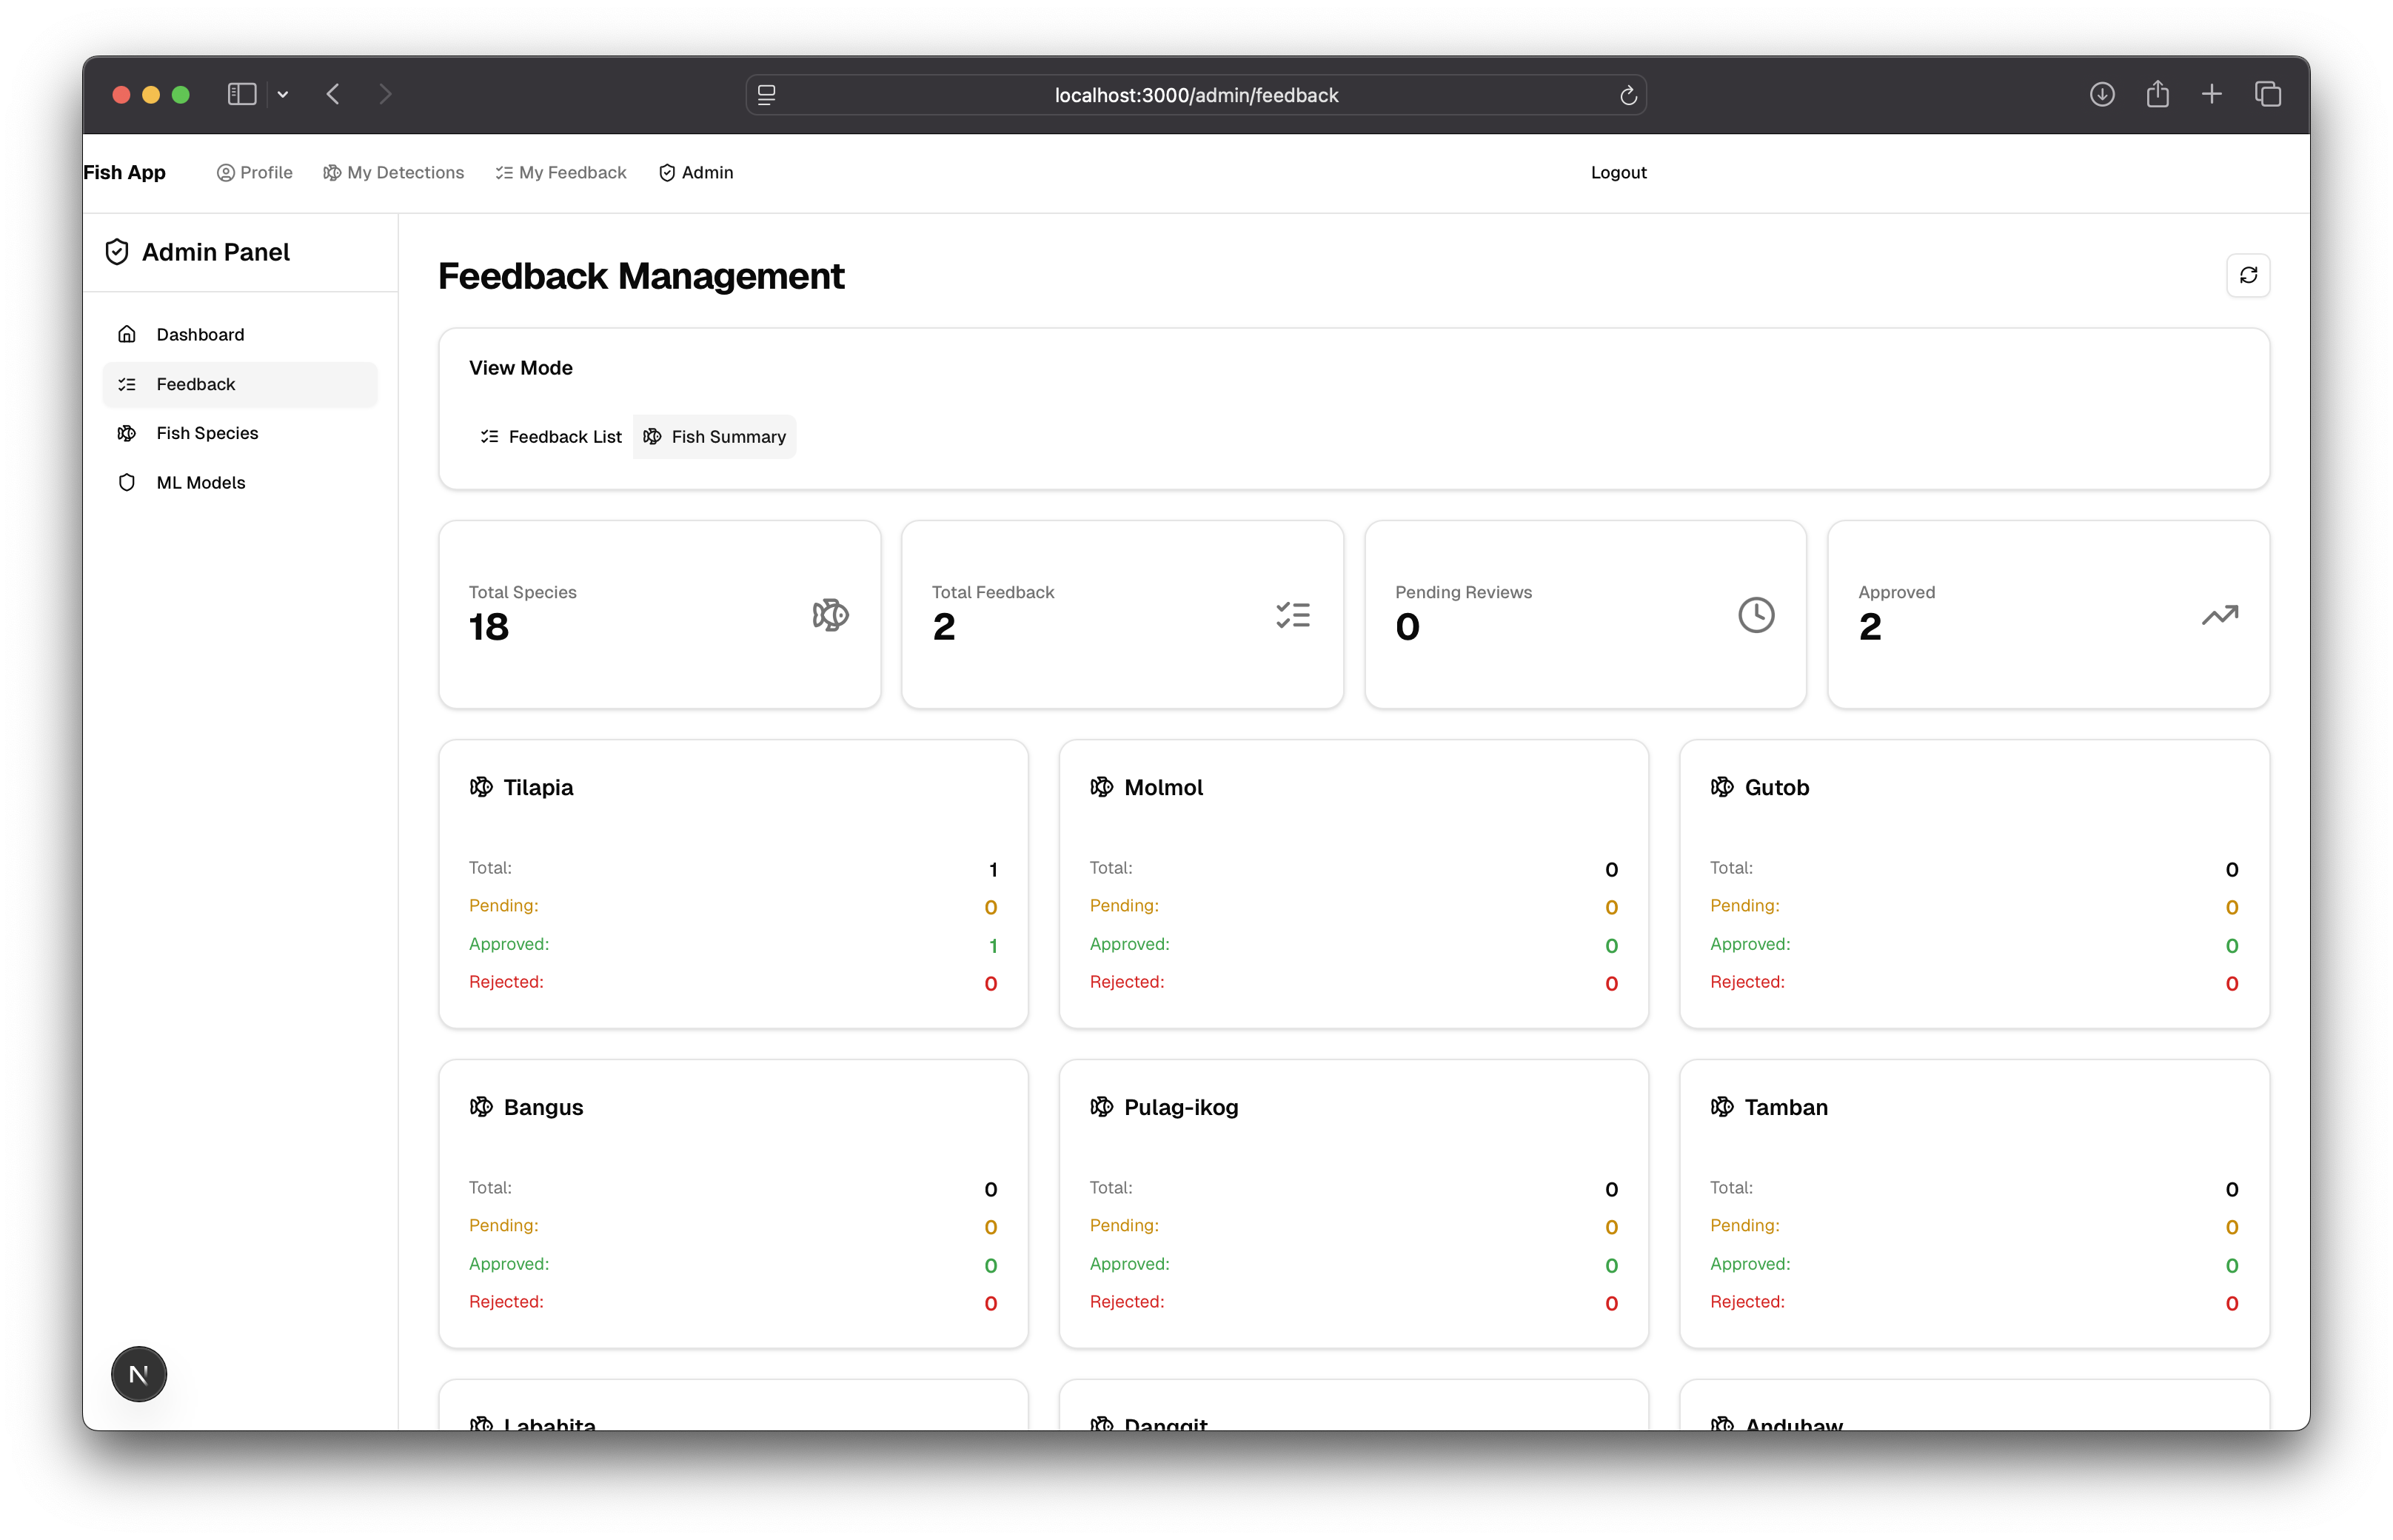
\includegraphics[width=1.2\textwidth]{images/images/mobile_app/revision/ListofAllSpeciesWithTheirData.png}%
    }
    \caption{Feedback Management: Fish Summaries }
\end{figure}

\subsection{Fish Summary Analytics}
The Feedback Management section includes analytics of the fish summary list, presenting the total number of species, total feedback submissions, pending reviews, and approved feedback. It also provides a detailed summary for each individual species, showing the total number of feedback submissions for that species along with the counts of feedback that are pending review, approved, and rejected.
\newpage

\begin{figure}[H]
    \makebox[\textwidth][c]{%
        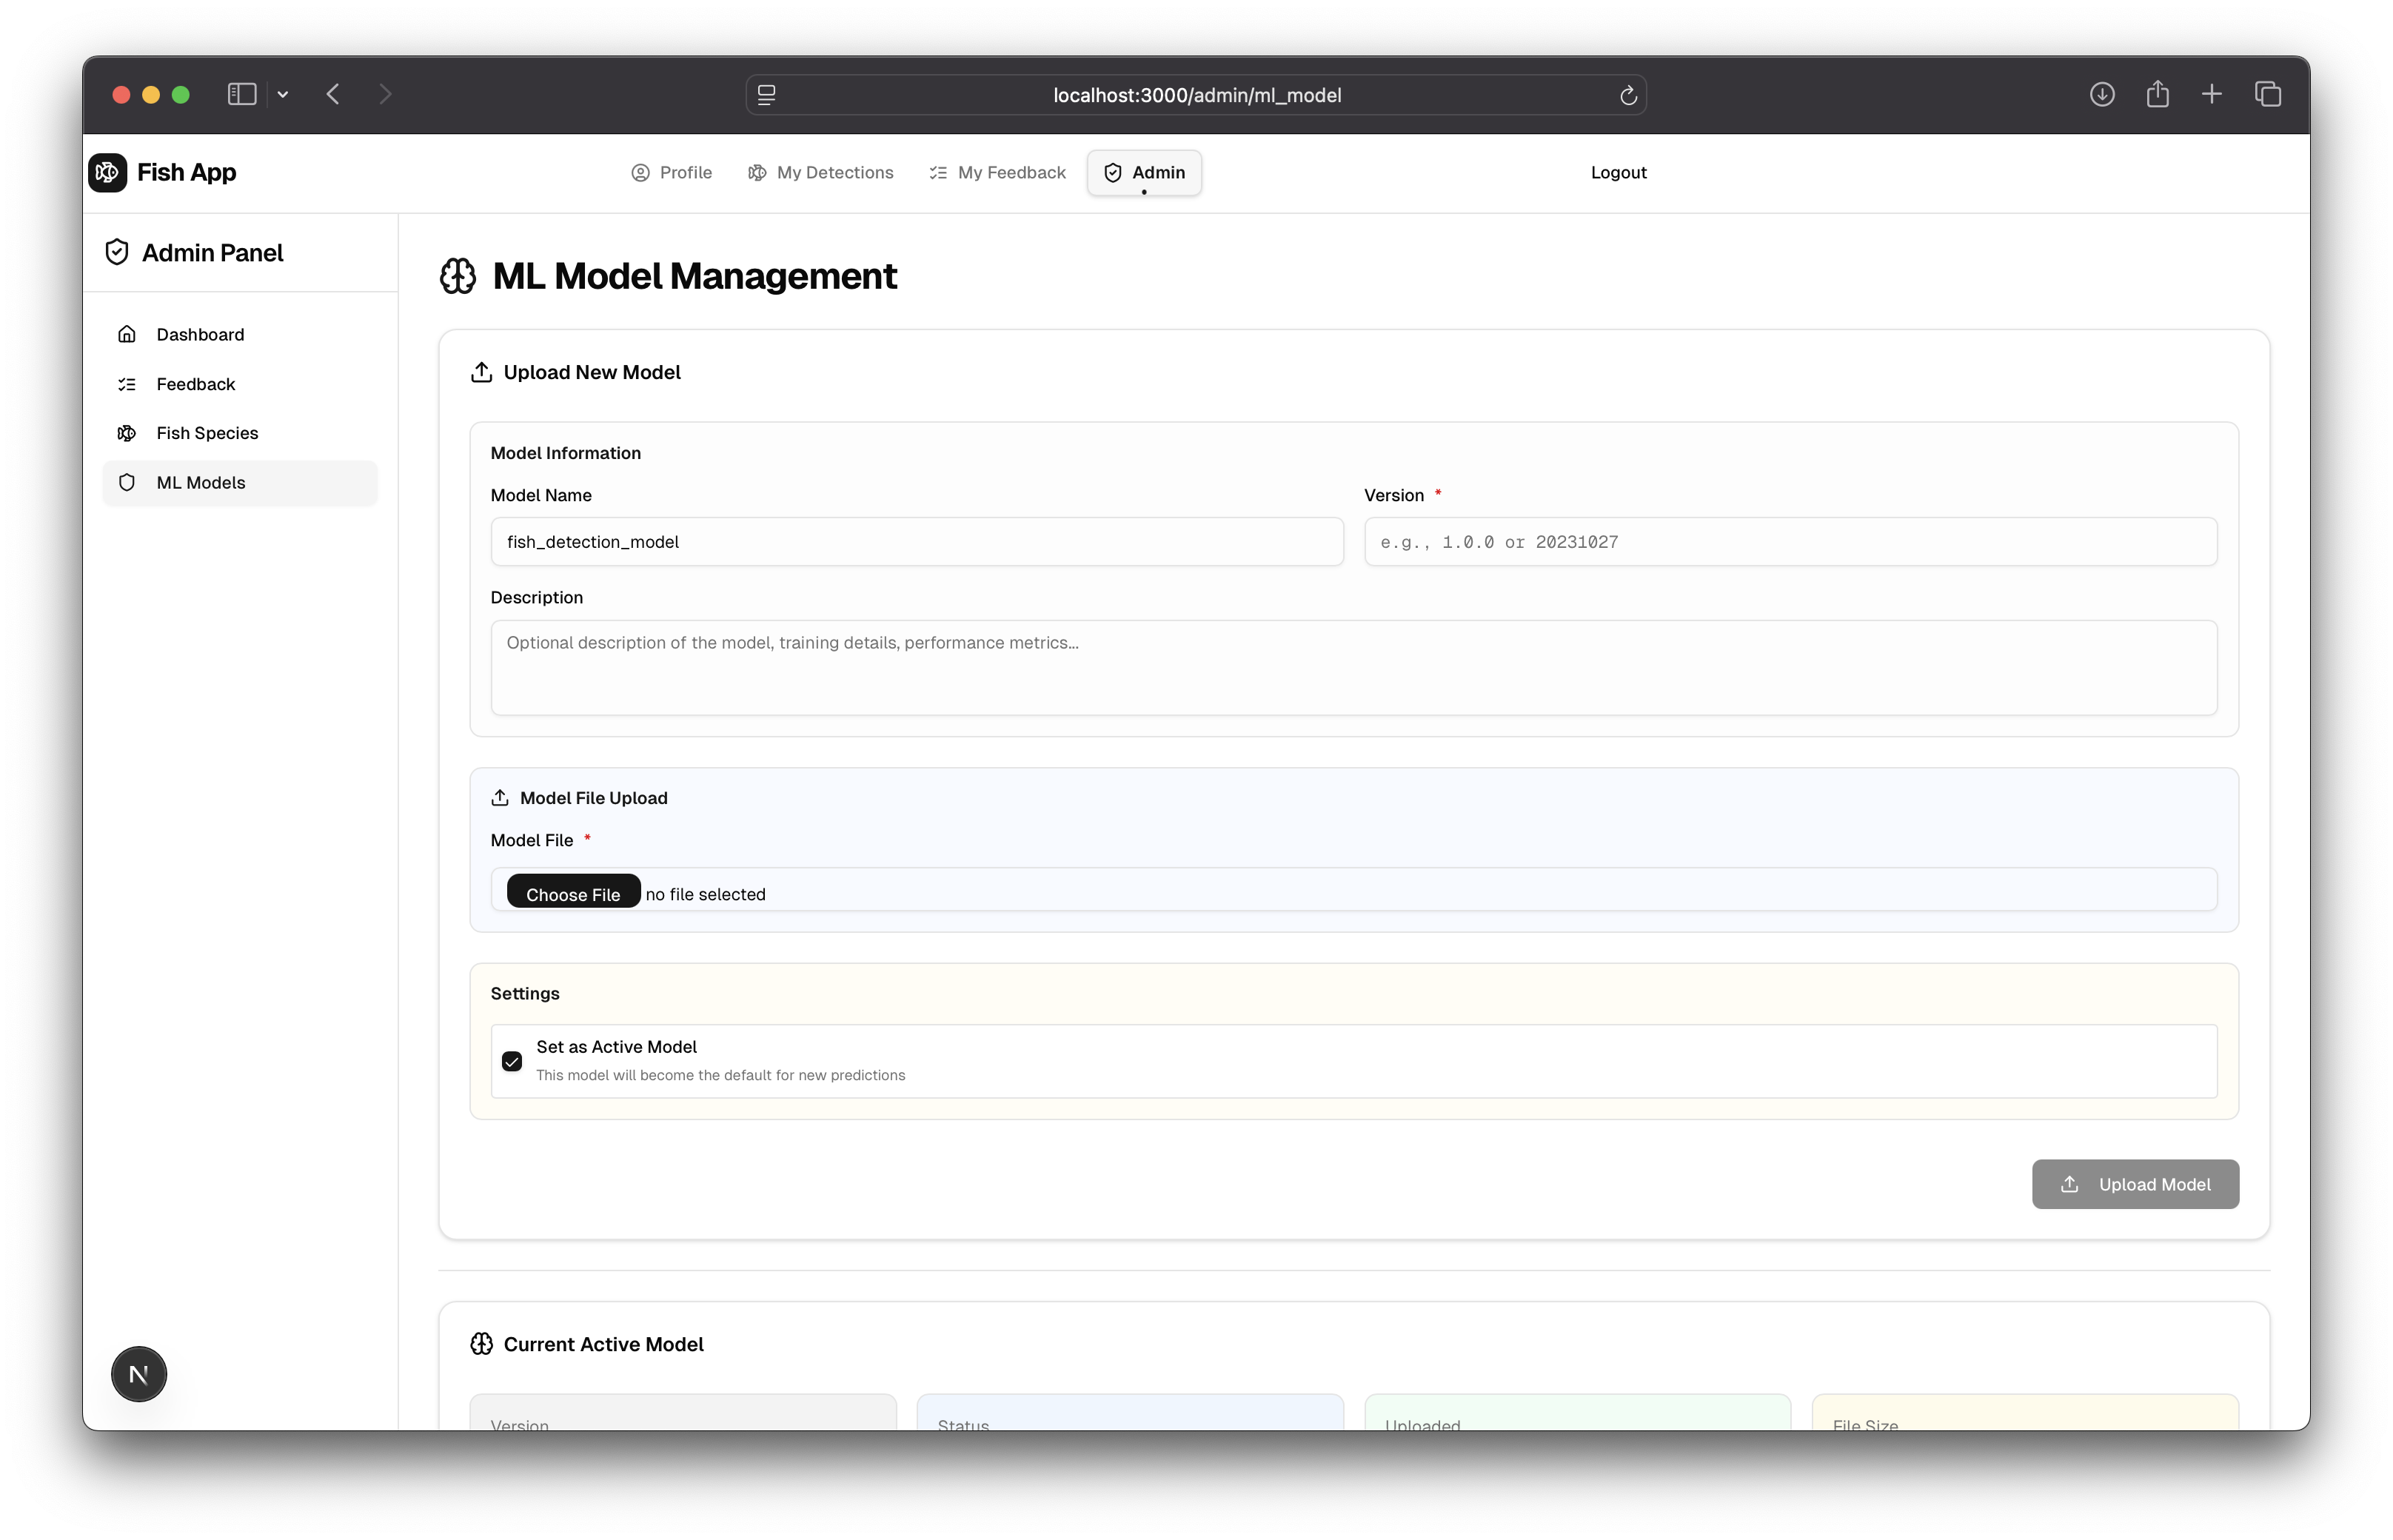
\includegraphics[width=1.2\textwidth]{images/images/mobile_app/revision/ModelUpload.png}%
    }
    \caption{Uploading Machine Learning Models}
\end{figure}

\subsection{Machine Learning Model Management}
In the ML Model Management section, the administrator can upload a new model by providing its name, version, and description. The newly uploaded model can also be designated as the active model, which will then serve as the default for all new predictions. This section additionally allows the administrator to view other available model versions along with their corresponding status, detailed information, and file size.
\newpage

\subsection{Summary: Achievement of Specific Objectives}
This study successfully fulfilled all the specific objectives outlined at the beginning of the research:

\begin{enumerate}
    \item \textbf{Image Collection}: A total of 2,700 raw images were collected from local wet markets in Iligan City, ensuring species diversity across 18 fish types under natural lighting conditions.

    \item \textbf{Dataset Annotation}: Each image was annotated using Label Studio, and class remapping ensured consistency across the dataset. This was crucial for preparing high-quality training data usable by the YOLOv11 algorithm.

    \item \textbf{Model Development}: The YOLOv11 model was developed and trained to detect and classify all 18 species. Techniques such as transfer learning and hyperparameter tuning were applied to enhance accuracy and efficiency.

    \item \textbf{Model Evaluation}: The system achieved a mean Average Precision (mAP@0.5) of 0.75, a precision of 0.72, recall of 0.68, and F1-score of 0.70, indicating reliable classification performance, especially under real-world mobile deployment scenarios.

    \item \textbf{Mobile Application Development}: A Flutter-based mobile application was developed with integrated real-time fish detection, ecological and nutritional information retrieval, and offline data access. The YOLOv11 model was deployed via TensorFlow Lite, ensuring compatibility and responsiveness on mobile devices.

    \item \textbf{User Feedback Mechanism}: A feedback feature was implemented within the mobile app, allowing users to confirm or correct detected species. This data is reviewed via a Django-powered web admin panel and is designed to support future model retraining for continuous improvement.
\end{enumerate}

In summary, the \textit{ClassiFish} system achieved its intended objectives, demonstrating the feasibility of a mobile fish classification application powered by deep learning. The combination of technical robustness and user engagement mechanisms positions the system for practical use in education, fisheries research, and community-driven conservation efforts.
